%!TEX TS-program = xelatex
% ******************************* PhD Thesis Template **************************
% Please have a look at the README.md file for info on how to use the template

%\documentclass[a4paper,12pt,customfont,numbered,print,index,draft]{Classes/PhDThesisPSnPDF}
\documentclass[a4paper,12pt,customfont,numbered,print,withindex,chapter,custombib]{Classes/PhDThesisPSnPDF}

% ******************************************************************************
% ******************************* Class Options ********************************
% *********************** See README for more details **************************
% ******************************************************************************

% `a4paper'(The University of Cambridge PhD thesis guidelines recommends a page
% size a4 - default option) or `a5paper': A5 Paper size is also allowed as per
% the Cambridge University Engineering Deparment guidelines for PhD thesis
%
% `11pt' or `12pt'(default): Font Size 10pt is NOT recommended by the University
% guidelines
%
% `oneside' or `twoside'(default): Printing double side (twoside) or single
% side.
%
% `print': Use `print' for print version with appropriate margins and page
% layout. Leaving the options field blank will activate Online version.
%
% `index': For index at the end of the thesis
%
% `draftclassic': For draft mode without loading any images (same as draft in book)
%
% `draft': Special draft mode with line numbers, images, and water mark with
% timestamp and custom text. Position of the text can also be modified.
%
% `abstract': To generate only the title page and abstract page with
% dissertation title and name, to submit to the Student Registry
%
% `chapter`: This option enables only the specified chapter and it's references
%  Useful for review and corrections.
%
% ************************* Custom Page Margins ********************************
%
% `custommargin`: Use `custommargin' in options to activate custom page margins,
% which can be defined in the preamble.tex. Custom margin will override
% print/online margin setup.
%
% *********************** Choosing the Fonts in Class Options ******************
%
% `times' : Times font with math support. (The Cambridge University guidelines
% recommend using times)
%
% `fourier': Utopia Font with Fourier Math font (Font has to be installed)
%            It's a free font.
%
% `customfont': Use `customfont' option in the document class and load the
% package in the preamble.tex
%
% default or leave empty: `Latin Modern' font will be loaded.
%
% ********************** Choosing the Bibliography style ***********************
%
% `authoryear': For author-year citation eg., Krishna (2013)
%
% `numbered': (Default Option) For numbered and sorted citation e.g., [1,5,2]
%
% `custombib': Define your own bibliography style in the `preamble.tex' file.
%              `\RequirePackage[square, sort, numbers, authoryear]{natbib}'.
%              This can be also used to load biblatex instead of natbib
%              (See Preamble)
%
% **************************** Choosing the Page Style *************************
%
% `default (leave empty)': For Page Numbers in Header (Left Even, Right Odd) and
% Chapter Name in Header (Right Even) and Section Name (Left Odd). Blank Footer.
%
% `PageStyleI': Chapter Name next & Page Number on Even Side (Left Even).
% Section Name & Page Number in Header on Odd Side (Right Odd). Footer is empty.
%
% `PageStyleII': Chapter Name on Even Side (Left Even) in Header. Section Number
% and Section Name in Header on Odd Side (Right Odd). Page numbering in footer

% Uncomment to change page style
%\pagestyle{PageStyleII}

% ********************************** Preamble **********************************
% Preamble: Contains packages and user-defined commands and settings
%!TEX root = ../thesis.tex
% !TEX TS-program = xelatex
% ****************************** Misc ******************************************
\usepackage{blindtext}
% ******************************************************************************
% ****************************** Custom Margin *********************************
% Add `custommargin' in the document class options to use this section
% Set {innerside margin / outerside margin / topmargin / bottom margin}  and
% other page dimensions
\ifsetCustomMargin
  \RequirePackage[left=37mm,right=30mm,top=35mm,bottom=30mm]{geometry}
  \setFancyHdr % To apply fancy header after geometry package is loaded
\fi

% Add spaces between paragraphs
%\setlength{\parskip}{0.5em}
% Ragged bottom avoids extra whitespaces between paragraphs
\raggedbottom
% To remove the excess top spacing for enumeration, list and description
%\usepackage{enumitem}
%\setlist[enumerate,itemize,description]{topsep=0em}

% *****************************************************************************
% ******************* Fonts (like different typewriter fonts etc.)*************
\usepackage{ wasysym }

% Add `customfont' in the document class option to use this section

\ifsetCustomFont
  % Set your custom font here and use `customfont' in options. Leave empty to
  % load computer modern font (default LaTeX font).
  \RequirePackage{mathpazo}
  \usepackage{amsmath}
  \usepackage{newpxtext}
  %\usepackage{mathpazo}
  %\usepackage[T1]{fontenc}
  %\usepackage{fontspec}

  \usepackage{sectsty}
  \usepackage{roboto}
  \allsectionsfont{\sffamily} % <---- omitting \bfseries still gives bold font
  %\usepackage{xfrac,fontspec,unicode-math}
  %\setmathfont[version=lm]{Latin Modern Math}
  % For use with XeLaTeX
  %  \setmainfont[
  %    Path              = ./libertine/opentype/,
  %    Extension         = .otf,
  %    UprightFont = LinLibertine_R,
  %    BoldFont = LinLibertine_RZ, % Linux Libertine O Regular Semibold
  %    ItalicFont = LinLibertine_RI,
  %    BoldItalicFont = LinLibertine_RZI, % Linux Libertine O Regular Semibold Italic
  %  ]
  %  {libertine}
  %  % load font from system font
  %  \newfontfamily\libertinesystemfont{Linux Libertine O}
\fi

% *****************************************************************************
% **************************** Custom Packages ********************************

% ************************* Algorithms and Pseudocode **************************

\usepackage{algpseudocode}


% ********************Captions and Hyperreferencing / URL **********************

% Captions: This makes captions of figures use a boldfaced small font.
%\RequirePackage[small,bf]{caption}

\RequirePackage[labelsep=space,tableposition=top,small,bf]{caption}
\renewcommand{\figurename}{Fig.} %to support older versions of captions.sty


% *************************** Graphics and figures *****************************

%\usepackage{rotating}
%\usepackage{wrapfig}

% Uncomment the following two lines to force Latex to place the figure.
% Use [H] when including graphics. Note 'H' instead of 'h'
%\usepackage{float}
%\restylefloat{figure}

% Subcaption package is also available in the sty folder you can use that by
% uncommenting the following line
% This is for people stuck with older versions of texlive
%\usepackage{sty/caption/subcaption}
\usepackage{subcaption}

% ********************************** Tables ************************************
\usepackage{booktabs} % For professional looking tables
\usepackage{multirow}

\usepackage{multicol}
\usepackage{longtable}
\usepackage{tabularx}


% *********************************** SI Units *********************************
\usepackage[allow-number-unit-breaks=true,separate-uncertainty=true,multi-part-units=single,binary-units=true]{siunitx} % use this package module for SI units

% ******************************* Line Spacing *********************************

% Choose linespacing as appropriate. Default is one-half line spacing as per the
% University guidelines

% \doublespacing
 \onehalfspacing
% \singlespacing

\usepackage{enumitem}

% ************************ Formatting / Footnote *******************************

% Don't break enumeration (etc.) across pages in an ugly manner (default 10000)
%\clubpenalty=500
%\widowpenalty=500

%\usepackage[perpage]{footmisc} %Range of footnote options


% *****************************************************************************
% *************************** Bibliography  and References ********************

%\usepackage{cleveref} %Referencing without need to explicitly state fig /table

% Add `custombib' in the document class option to use this section
% \ifuseCustomBib
   % \RequirePackage[numbers,sort&compress]{natbib} % CustomBib

% If you would like to use biblatex for your reference management, as opposed to the default `natbibpackage` pass the option `custombib` in the document class. Comment out the previous line to make sure you don't load the natbib package. Uncomment the following lines and specify the location of references.bib file


\RequirePackage[style=nature,date=year,backend=bibtex,doi=false,isbn=false,url=false,sorting=none,sortcites=true,doi=false,url=false,hyperref]{biblatex}
\addbibresource{./References/references.bib,./References/references.bib} %Location of references.bib only for biblatex, Do not omit the .bib extension from the filename.
\bibliography{References/references,References/_references} %Location of references.bib only for biblatex

% \fi

% changes the default name `Bibliography` -> `References'
\renewcommand{\bibname}{References}


% ******************************************************************************
% ************************* User Defined Commands ******************************
% ******************************************************************************

% *********** To change the name of Table of Contents / LOF and LOT ************

%\renewcommand{\contentsname}{My Table of Contents}
%\renewcommand{\listfigurename}{My List of Figures}
%\renewcommand{\listtablename}{My List of Tables}


% ********************** TOC depth and numbering depth *************************

\setcounter{secnumdepth}{2}
\setcounter{tocdepth}{2}


% ******************************* Nomenclature *********************************

% To change the name of the Nomenclature section, uncomment the following line

%\renewcommand{\nomname}{Symbols}


% ********************************* Appendix ***********************************

% The default value of both \appendixtocname and \appendixpagename is `Appendices'. These names can all be changed via:

%\renewcommand{\appendixtocname}{List of appendices}
%\renewcommand{\appendixname}{Appndx}

% *********************** Configure Draft Mode **********************************

% Uncomment to disable figures in `draft'
%\setkeys{Gin}{draft=true}  % set draft to false to enable figures in `draft'

% These options are active only during the draft mode
% Default text is "Draft"
%\SetDraftText{DRAFT}

% Default Watermark location is top. Location (top/bottom)
%\SetDraftWMPosition{bottom}

% Draft Version - default is v1.0
%\SetDraftVersion{v1.1}

% Draft Text grayscale value (should be between 0-black and 1-white)
% Default value is 0.75
%\SetDraftGrayScale{0.8}


% ******************************** Todo Notes **********************************
%% Uncomment the following lines to have todonotes.

\ifsetDraft
	\usepackage[colorinlistoftodos]{todonotes}
	\newcommand{\mynote}[1]{\todo[author=ctr26,size=\small,inline,color=green!40]{#1}}
\else
	\newcommand{\mynote}[1]{}
	\newcommand{\listoftodos}{}
\fi

% Example todo: \mynote{Hey! I have a note}

%%%
\usepackage{pgfplots}
\usepackage{tikzscale}
\usepackage{helvet}

\usepackage[eulergreek]{sansmath}
\pgfplotsset{
  tick label style = {font=\sansmath\sffamily\footnotesize},
  %every axis label = {font=\sansmath\sffamily},
  %legend style = {font=\sansmath\sffamily},
  %label style = {font=\sansmath\sffamily}
}
\usepackage{roboto}
% https://github.com/matlab2tikz/matlab2tikz/issues/672
\newlength{\figwidth}
\newlength{\figheight}

\setlength{\figwidth}{0.4\textwidth}
\setlength{\figheight}{0.6180\figwidth}


\usepackage{graphicx}
\usepackage{xcolor}
\definecolor{darkblue}{rgb}{0,0,0.5}
\usepackage{transparent}

\usepackage{import}

\usepackage{pdflscape}

\usepackage{dpfloat}
\usepackage{multicol}

\usepackage{mhchem}
\usepackage{wrapfig}
\usepackage[super]{nth}


\newcommand{\nosection}[1]{%
  \refstepcounter{section}%
  \addcontentsline{toc}{section}{\protect\numberline{\thesection}#1}%
  \markright{#1}}


  \usepackage{tikz}
  \usepackage{graphicx}
  \usetikzlibrary{positioning}

%!TEX root = ../thesis.tex

% \usepackage{makeidx}

\makeglossaries{}
\makeindex

\setabbreviationstyle[acronym]{long-short}
\glssetcategoryattribute{acronym}{dualindex}{true}
\glssetcategoryattribute{general}{dualindex}{true}

% Symbols
\glsxtrnewsymbol[description={Field of View}]{FOV}{FOV}
\glsxtrnewsymbol[description={Rayleigh length}]{z_R}{\ensuremath{z_R}}
\glsxtrnewsymbol[description={Confocal parameter}]{b}{\ensuremath{b}}
\glsxtrnewsymbol[description={Half angle of the entrance pupil of a lens}]{alpha}{\ensuremath{\alpha}}
\glsxtrnewsymbol[description={Bessel function of the first kind}]{J_1}{\ensuremath{J_1}}
\glsxtrnewsymbol[description={Fluorescent molecule lifetime as a half life}]{tau}{\ensuremath{\tau_{\frac{1}{2}}}}
\glsxtrnewsymbol[description={Spot size of \gls{Gaussian beam}, waist}]{omega_0}{\ensuremath{\omega_0}}
\glsxtrnewsymbol[description={Wavelength}]{lambda}{\ensuremath{\lambda}}
\glsxtrnewsymbol[description={Numerical aperture}]{NA}{NA}
\glsxtrnewsymbol[description={Electric field}]{E}{\ensuremath{E}}
\glsxtrnewsymbol[description={Intensity,~\(\gls{E}^2\)}]{I}{\ensuremath{I}}
\glsxtrnewsymbol[description={Spot size of a Gaussian beam}]{w_0}{\ensuremath{w_0}}
\glsxtrnewsymbol[description={Field number, diameter of the eyepiece lens}]{F_n}{\ensuremath{F_{\text{n}}}}


%Computer vision
\glsxtrnewsymbol[description={World coordinates, \((X, Y, Z)\)}]{X}{\ensuremath{\mathbf{X}}}
\glsxtrnewsymbol[description={Camera-centered world coordinate,\((X_c, Y_c, Z_c)\), left camera}]{X_c}{\ensuremath{\mathbf{X_c}}}
\glsxtrnewsymbol[description={Camera-centered world coordinate,\((X_c', Y_c', Z_c')\) right camera}]{X_c'}{\ensuremath{\mathbf{X_c'}}}
\glsxtrnewsymbol[description={Ray to point on image plane,\((x,y,f)\), left camera}]{p}{\ensuremath{\mathbf{p}}}
\glsxtrnewsymbol[description={Ray to point on image plane,\((x,y,f)\), right camera}]{p'}{\ensuremath{\mathbf{p'}}}
\glsxtrnewsymbol[description={Image plane coordinates,\((x,y)\), left camera}]{x}{\ensuremath{\mathbf{x}}}
\glsxtrnewsymbol[description={Image plane coordinates,\((x,y)\), right camera}]{x'}{\ensuremath{\mathbf{x'}}}
\glsxtrnewsymbol[description={Pixel coordinates,\((u,v)\), left camera}]{w}{\ensuremath{\mathbf{w}}}
\glsxtrnewsymbol[description={Pixel coordinates,\((u,v)\), right camera}]{w'}{\ensuremath{\mathbf{w'}}}
\glsxtrnewsymbol[description={Camera parameters, left camera}]{K}{\ensuremath{\mathbf{K}}}
\glsxtrnewsymbol[description={Camera parameters, right camera}]{K'}{\ensuremath{\mathbf{K'}}}

\glsxtrnewsymbol[description={Rotation matrix (orthonormal)}]{R}{\ensuremath{\mathbf{R}}}
\glsxtrnewsymbol[description={Translation vector (3 element)}]{T}{\ensuremath{\mathbf{T}}}
\glsxtrnewsymbol[description={The Fundamental matrix}]{F}{\ensuremath{\mathbf{F}}}
\glsxtrnewsymbol[description={The Essential matrix}]{Essential}{\ensuremath{\mathbf{E}}}
\glsxtrnewsymbol[description={The Homography matrix}]{H}{\ensuremath{\mathbf{H}}}
\glsxtrnewsymbol[description={\(3\times3\) matrix containing coordinates from \gls{T}}]{T_x}{\ensuremath{\mathbf{T_\times}}}
\glsxtrnewsymbol[description={Mean square error: \(\operatorname{MSE}=\frac{1}{n}\sum_{i=1}^n{(Y_i-\hat{Y_i})}^2\)}]{MSE}{\ensuremath{MSE}}

\glsxtrnewsymbol[description={Tissue viscosity}]{eta_1_visc}{\ensuremath{\eta_1}}
\glsxtrnewsymbol[description={Cellular viscosity}]{eta_2_visc}{\ensuremath{\eta_2}}
\glsxtrnewsymbol[description={Time constant of the tissue}]{tau_visc}{\ensuremath{\tau}}
\glsxtrnewsymbol[description={Ensemble stiffness}]{E_visc}{\ensuremath{E}}

% Mean Square Error
% Glossary

\newglossaryentry{4f}{
    name={4f},
    description={Two lens system with each plane separated by a focal length \(f \)}
}
\newglossaryentry{primary imaging plane}{
    name={primary imaging plane},
    description={The first plane where a true image is relayed.}
}
\newglossaryentry{objective lens}{
    name={objective lens},
    description={The collecting lens nearest the sample}
}
\newglossaryentry{specificity}{
    name={specificity},
    description={The ability of fluorescent imaging to label specific aspects of a sample}
}
\newglossaryentry{depth of field}{
    name={depth of field},
    description={The axial range about a lens' focal plane where an image sample will continued to keep focus.}
}
\newglossaryentry{airy disk}{
    name={Airy disk},
    description={Theoretical lateral intensity distribution of a point emitter}
}
\newglossaryentry{nyquist sampling theory}{
    name={Nyquist sampling theory},
    description={The resolution of the detector required to resample the image information faithfully is twice the bandwidth of the sampled signal.}
}
\newglossaryentry{stokes shift}{
    name={stoke shift},
    description={The red shift in colour of fluorescent molecules when emission light is compared to excitation light.}
}
\newglossaryentry{autophagy}{
    name={autophagy},
    description={The mechanism by which cells disassemble.}
}
\newglossaryentry{lysosome}{
    name={lysosome},
    description={Organelle within the cell where enzymes are kept for degrading molecules}
}
\newglossaryentry{transfection}{
    name={transfection},
    description={The process by which external matter is inserted into the cell}
}
\newglossaryentry{etendue}{
    name={etendue},
    description={A property of propagating light which is conversed and is defined as the product solid angle of of the system's entrance pupil and the area}
}
\newglossaryentry{coherent}{
    name={coherent},
    description={The distance over which a photons from the same source will stay in phase}
}
\newglossaryentry{super-continuum laser}{
    name={super-continuum laser},
    description={A source of white laser light, achieved using non-linear effects in a photonic crystal fibre and a pump laser.}
}
\newglossaryentry{pixel}{
    name={pixel},
    description={Picture element}
}
\newglossaryentry{photosite}{
    name={photosite},
    description={Single light recording element of an array forming an imaging detector}
}

\newglossaryentry{wide-field}{
    name={wide-field},
    description={The entire area of interest is exposed to light and recorded at once}
}
\newglossaryentry{quantum efficiency}{
    name={quantum efficiency},
    description={The photonic to electron conversion rates, the \emph{yield} of the detector}
}
\newglossaryentry{dynamic range}{
    name={dynamic range},
    description={The ratio between the largest and smallest intensity values that a photo-site can assume}
}
\newglossaryentry{bit depth}{
    name={bit depth},
    description={The resolution in bits of a digitally converted measurand}
}
\newglossaryentry{dark current}{
    name={dark current},
    description={The residual electric current flowing in each photo-site when there is no incident illumination}
}
\newglossaryentry{read noise}{
    name={read noise},
    description={Noise contribution from the electronics within the camera}
}
\newglossaryentry{photon noise}{
    name={photon noise},
    description={The intrinsic variation of the incident photon flux}
}
\newglossaryentry{poissonian distribution}{
    name={poissonian distribution},
    description={Discrete probability distribution in a fixed epoch}
}
\newglossaryentry{fluorophore}{
    name={fluorophore},
    description={Fluorescent molecule: chromophore, fluorochrome}
}
\newglossaryentry{photosensitier}{
    name={photosensitier},
    description={Molecules which produce chemical change is surrounding molecules using photon energy}
}
\newglossaryentry{confocal microscope}{
    name={confocal microscope},
    description={A laser scanning microscope wherein an adjustable pinhole is placed at a conjugate imaging plane to control axial and spatial resolution of the reconstructed image}
}
\newglossaryentry{confocal}{
    name={confocal},
    description={Common focal point between lenses, similiar to conjugate planes}
}
\newglossaryentry{galvanometric scanning mirrors}{
    name={galvanometric scanning mirrors},
    description={Voltage controlled mirrors where voltage is proportional to angle}
}
\newglossaryentry{resonant scanning mirrors}{
    name={resonant scanning mirrors},
    description={Voltage controlled mirrors driven at their resonant frequency to increase the maximum viable scanning speed}
}
\newglossaryentry{photobleaching}{
    name={photobleaching},
    description={The ensemble reduction in fluorescent intensity as individual \gls{fluorophore}s lose the ability to fluoresce}
}
\newglossaryentry{photo-toxicity}{
    name={photo-toxicity},
    description={Damage caused to a biological sample due to light}
}
\newglossaryentry{aberration}{
    name={aberration},
    description={Distortions caused in an image by imperfect optics in the imaging system}
}
\newglossaryentry{Fourier transform}{
    name={Fourier transform},
    description={Coordinate transform to convert points in real space into points in frequency space}
}
\newglossaryentry{missing cone}{
    name={missing cone},
    description={The cone of space missing in the 3D \gls{OTF}}
}
\newglossaryentry{super-resolution}{
    name={super-resolution},
    description={Imaging at resolutions beyond the diffraction limit}
}
\newglossaryentry{light-sheet}{
    name={light-sheet},
    description={A thin plane of light}
}
\newglossaryentry{convolution theorem}{
    name={convolution theorem},
    description={The relation between convolution in Cartesian space versus multiplication in frequency space, see Appendix~\ref{appendix:convolution_theorem}}
}
\newglossaryentry{epi-fluorescence}{
    name={epi-fluorescence},
    description={Fluorescence microscopy imaged along the same optics used to illuminate}
}
\newglossaryentry{optical sectioning}{
    name={optical sectioning},
    description={The ability of a microscope to image axial slices of a thick sample}
}
\newglossaryentry{ultra-microscope}{
    name={ultra-microscope},
    description={A light-sheet microscope for observing small particles or colloids using scattered light, developed by R. A. Zsigmondy 1902}
}
\newglossaryentry{openSPIM}{
    name={openSPIM},
    description={Open hardware project of documentation to help home-users build their own \gls{SPIM}}
}
\newglossaryentry{Gaussian beam}{
    name={Gaussian beam},
    description={Model that governs the propagation of \emph{vanilla} coherent \gls{Laser} sources with no phase of illumination shaping optics.}
}
\newglossaryentry{Lorentzian}{
    name={Lorentzian},
    description={\(f(x) = \frac{1}{x^2+1}\)
    }
}
\newglossaryentry{Rayleigh length}{
    name={Rayleigh length},
    description={The distance along the propagation direction of a Gaussian beam where the beam is percieved to be still collimated.
    }
}
\newglossaryentry{virtual light-sheet}{
    name={virtual light-sheet},
    description={\Gls{light-sheet} generated by spatially sweeping a beam}
}
% \newglossaryentry{tele-centric}{
%     name={tele-centric},
%     description={A lens property where all the chief rays are collimated and parallel to the optical axis}
% }
\newglossaryentry{working distance}{
    name={working distance},
    description={The distance an objective needs to be away from a sample to keep focus, distance to the focal plane}
}
\newglossaryentry{tomography}{
    name={tomography},
    description={Tomography is imaging of a sample by sections or sectioning using waves}
}
\newglossaryentry{Spatial Light Modulator}{
    name={Spatial Light Modulator},
    description={Array device for modulating phase and/or intensity of incident light}
}
\newglossaryentry{exotic beam}{
    name={exotic beam},
    description={Non-Gaussian beams with structure and exploitable properties}
}
\newglossaryentry{axicon}{
    name={axicon},
    description={Lens with a conical surface}
}
\newglossaryentry{Bessel beam}{
    name={Bessel beam},
    description={Non-diffraction, self-healing beam. Narrow central lobe with multiple outer orders}
}
\newglossaryentry{Airy beam}{
    name={Airy beam},
    description={Non-diffraction, self-healing beam. Appears to bend}
}
\newglossaryentry{comatic aberration}{
    name={comatic aberration},
    description={Abberation caused from imaging off-axis}
}
\newglossaryentry{lattice light-sheet}{
    name={lattice light-sheet},
    description={Lattice of self-reinforced Bessel beams, narrowed into a sheet}
}
\newglossaryentry{deconvolution}{
    name={deconvolution},
    description={The mathematical reversing of convolution. Improves image fidelity}
}
\newglossaryentry{Laser}{
    name={laser},
    description={Light Amplification by Stimulated Emission}
}
\newglossaryentry{LabVIEW}{
    name={LabVIEW},
    description={Graphical programming language for lab rapid development instrumentation}
}
\newglossaryentry{imaging board}{
    name={imaging board},
    description={Top most breadboard, holding imaging and illumination optics}
}
\newglossaryentry{illumination board}{
    name={illumination board},
    description={Bottom most breadboard, holding illumination sources and optics}
}
\newglossaryentry{imaging optical rail}{
    name={imaging optical rail},
    description={Optical rail holing camera and filter wheel}
}
\newglossaryentry{detection arm}{
    name={detection arm},
    description={\SI{45}{\degree} opts-mechanics rail on the imaging board holding detection optics}
}
\newglossaryentry{illumination arm}{
    name={illumination arm},
    description={\SI{45}{\degree} opts-mechanics rail on the imaging board holding illumination optics}
}
\newglossaryentry{telecentric}{
    name={telecentric},
    description={A lens property where all the chief rays are collimated and parallel to the optical axis}
}
\newglossaryentry{state machine}{
    name={state machine},
    description={A model of computation containing a finite number of possible states of which it may only exist in one at any time.}
}
\newglossaryentry{producer-consumer architecture}{
    name={producer-consumer architecture},
    description={Parallel running \gls{state machine}s, where the producer machine sends commands and data to the consumer machine}
}
\newglossaryentry{queueing architecture}{
    name={queueing architecture},
    description={Operations and data are queued into a register for action upon from a state machine. Queues may be first in first out, first in last out etc.}
}
\newglossaryentry{race conditions}{
    name={race conditions},
    description={When system attempts to perform two or more operations at the same time}
}
\newglossaryentry{enumerated type}{
    name={enumerated type},
    description={A variable which acts as an identifer and acts as a constant value}
}
\newglossaryentry{exposure time}{
    name={exposure time},
    description={Integration time of a single recorded frame}
}
\newglossaryentry{exposure}{
    name={exposure},
    description={Exposure time \(\times \) gain}
}
\newglossaryentry{background signal}{
    name={background signal},
    description={Additional signal from the environment, specimen or system which contributes to lowering the \gls{SNR}}
}
\newglossaryentry{homography}{
    name={homography},
    description={A projective transform}
}
\newglossaryentry{Ram-Lak filter}{
    name={Ram-Lak filter},
    description={Linear real (amplitude) ramp filter in Fourier space}
}
\newglossaryentry{sinugram}{
    name={sinogram},
    description={The image of Cartesian as transformed into angular space}
}
% \newglossaryentry{homography matrix}{
%     name={homography matrix},
%     description={DEFINE}
% }
\newglossaryentry{homogeneous coordinates}{
    name={homogeneous coordinates},
    description={A higher dimensional representation of lower dimensional coordinates to facilitate non-linear operations}
}
\newglossaryentry{zebrafish}{
    name={zebrafish},
    description={\emph{Danio rerio}. A model organism  ubiquitous in light-sheet imaging}
}
\newglossaryentry{chorion}{
    name={chorion},
    description={The soft membrane surrounding embryos}
}
\newglossaryentry{sample plane}{
    name={sample plane},
    description={Plane in sample as imaged onto the imaging plane of an optical system}
}
\newglossaryentry{world point}{
    name={world point},
    description={A point in world-centered coordinates}
}
\newglossaryentry{essential matrix}{
    name={essential matrix},
    description={\(3\times 3\) matrix which relates corresponding points in stereo image pairs in calibrated cameras}
}
\newglossaryentry{fundamental matrix}{
    name={fundamental matrix},
    description={\(3\times 3\) matrix which relates corresponding points in stereo image pairs}
}
\newglossaryentry{image plane}{
    name={image plane},
    description={Image one focal distance away from the camera-centered coordinates along the optical axis}
}
\newglossaryentry{Radon transform}{
    name={Radon transform},
    description={Integral transform converting Cartesian space into angular space along one axis}
}
\newglossaryentry{agarose VII}{
    name={agarose VII},
    description={Optical clear hydrated gel. This type of agarose is the closest matching refractive index to that of water}
}
\newglossaryentry{slit-scanning}{
    name={slit-scanning},
    description={The scanning of a narrow slit to increase contrast and resolution along the direction orthogonal to the slit direction}
}
\newglossaryentry{3D printing}{
    name={3D printing},
    description={Additive method of building shapes, often using hot malleable plastic extrusions}
}
% \newglossaryentry{ABS}{
%     name={ABS},
%     description={DEFINE}
% }
% \newglossaryentry{PLA}{
%     name={PLA},
%     description={DEFINE}
% }
\newglossaryentry{organoid}{
    name={organoid},
    description={A miniature and simplified organ}
}
\newglossaryentry{SH-SY5Y}{
    name={SH-SY5Y},
    description={Human derived neuronal cell line}
}
\newglossaryentry{open-hardware}{
    name={open-hardware},
    description={Freely and open available designs for hardware}
}
\newglossaryentry{virion}{
    name={virion},
    description={A single virus particle}
}
\newglossaryentry{capsid}{
    name={capsid},
    description={Protein shell of a virus}
}
\newglossaryentry{VP26}{
    name={VP26},
    description={Structural protein found in the capsid}
}
\newglossaryentry{VP1/2}{
    name={VP1/2},
    description={Structural protein found in the capsid}
}
\newglossaryentry{VP16}{
    name={VP16},
    description={Tegument protein which complexes with host DNA to induce gene transcription, the initiation of gene expression}
}
%\gls{background fluorescence}
% Acronyms

% \newacronym{FOV}{FOV}{Field of View}
\newacronym{sCMOS}{sCMOS}{scientific Complementary Metal-Oxide-Semiconductor}
% \newacronym{NA}{NA}{Numerical Aperture}
\newacronym{SNR}{SNR}{Signal to Noise ratio}
\newacronym{CCD}{CCD}{Charge-coupled device}
\newacronym{ICCD}{ICCD}{Intensified Charge-coupled device}
% \newacronym{Laser}{Laser}{Light Amplification by Stimulated Emission}
\newacronym{LED}{LED}{Light Emitting Diode}
\newacronym{EMCCD}{EMCCD}{Electron-Multiplying Charge-Coupled Device}
\newacronym{CMOS}{CMOS}{Complementary Metal-Oxide-Semiconductor}
\newacronym{FRAP}{FRAP}{Fluorescence Recovery After Photobleaching}
\newacronym{2P}{2P}{2-Photon}
\newacronym{SIM}{SIM}{Structured Illumination Microscopy}
\newacronym{iSIM}{iSIM}{instant Structured Illumination Microscopy}
\newacronym{mSIM}{mSIM}{multi-focal Structured Illumination Microscopy}
\newacronym{OTF}{OTF}{Optical Transfer Function}
\newacronym{LSFM}{LSFM}{\Gls{light-sheet} Fluorescence Microscopy}
\newacronym{SPIM}{SPIM}{Selective Plane Imaging Microscope}
\newacronym{FWHM}{FWHM}{Full-Width at Half-Maximum}
\newacronym{DSLM}{DSLM}{Digitally scanned Light-Sheet Microscopy}
\newacronym{ETL}{ETL}{Electronically Tuneable Lens}
\newacronym{iSPIM}{iSPIM}{inverted Selective-Plane Imaging Microscope}
\newacronym{LWD}{LWD}{Long Working Distance}
\newacronym{diSPIM}{diSPIM}{dual inverted Selective-Plane Imaging Microscope}
\newacronym{MuVi-SPIM}{MuVi-SPIM}{Multiview Selective-Plane Illumination Microscope}
\newacronym{OPM}{OPM}{Oblique Plane Microscopy}
\newacronym{SLM}{SLM}{\gls{Spatial Light Modulator}}
\newacronym{PSF}{PSF}{Point Spread Function}
\newacronym{STED}{STED}{Simulated Emission Depletion}
\newacronym{mSPIM}{mSPIM}{multidirectional Selective Plane Illumination Microscopy}
\newacronym{SCAPE}{SCAPE}{Swept Confocally-Aligned Planar Excitation}
\newacronym{3D}{3D}{Three Dimensional}
\newacronym{2D}{2D}{Two Dimensional}
\newacronym{AOTF}{AOTF}{Acousto-Optic Tunable Filter}
% \newacronym{LabVIEW}{LabVIEW}{Laboratory Virtual Instrument Engineering Workbench}
\newacronym{TTL}{TTL}{Transistor-Transistor Logic}
\newacronym{DAQ}{DAQ}{Data Acquisition}
\newacronym{RS232}{RS232}{Recommended Standard 232}
\newacronym{FEP}{FEP}{Fluorinated Ethylene Propylene}
\newacronym{CAD}{CAD}{Computer Aided Design}
\newacronym{OPT}{OPT}{Optical Projection Tomography}
\newacronym{eOPT}{eOPT}{emission Optical Projection Tomography}
\newacronym{tOPT}{tOPT}{transmission Optical Projection Tomography}
\newacronym{SVD}{SVD}{Singular Value Decomposition}
\newacronym{SPT}{SPT}{Single Particle Tracking}
\newacronym{FFT}{FFT}{Fast Fourier Transform}
\newacronym{PBS}{PBS}{Phosphate-Buffered Saline}
\newacronym{HSV}{HSV}{Herpes Simplex Virus}
\newacronym{INM}{INM}{Inner Nuclear Membranes}
\newacronym{ONM}{ONM}{Outer Nuclear Membranes}
\newacronym{TIRF}{TIRF}{Total Internal Reflection Fluorescence}
\newacronym{PFV}{PFV}{Prototype Foamy Virus}
\newacronym{HILO}{HILO}{Highly Inclined and Laminated Optical sheet}
\newacronym{dSTORM}{dSTORM}{\emph{direct} stochastic optical reconstruction microscopy}
\newacronym{NN}{NN}{Neural Network}
\newacronym{EM}{EM}{Electron Microscopy}
\newacronym{AFM}{AFM}{Atomic Force Microscopy}
\newacronym{FLIM}{FLIM}{Fluorescence Lifetime Imaging Microscopy}
\newacronym{ABS}{ABS}{Acrylonitrile Butadiene Styrene}
\newacronym{PLA}{PLA}{Polylactic acid}
\newacronym{RAM}{RAM}{Random Access Memory}
\newacronym{WD}{WD}{Working distance}

\newacronym{Rac1}{Rac1}{Ras-related C3 botulinum toxin substrate 1}
\newacronym{DNRAC}{DNRAC}{dominant-negative Rac1gene construct}
\newacronym{DNROCK}{DNROCK}{dominant-negative Rho-kinase construct}
\newacronym{MoECad}{MoECad}{Ras-related C3 botulinum toxin substrate 1}
\newacronym{RhoA}{RhoA}{Ras homolog gene family, member A}
\newacronym{WT}{WT}{wild type}
\newacronym{GFP}{GFP}{Green Fluorescent Protein}
\newacronym{PFA}{PFA}{paraformaldehyde}
\newacronym{flOPT}{flOPT}{frame localisation Optical Projection Tomography}
% \newacronym{MoECad}{MoECad}{}
% \newacronym{LWD}{LWD}{Long Working Distance}

% ************************ Thesis Information & Meta-data **********************
% Thesis title and author information, refernce file for biblatex
% ************************ Thesis Information & Meta-data **********************
%% The title of the thesis
\title{Writing your PhD thesis in \texorpdfstring{\\ \LaTeX2e}{LaTeX2e}}
%\texorpdfstring is used for PDF metadata. Usage:
%\texorpdfstring{LaTeX_Version}{PDF Version (non-latex)} eg.,
%\texorpdfstring{$sigma$}{sigma}

%% Subtitle (Optional)
\subtitle{Using the CUED template}

%% The full name of the author
\author{Krishna Kumar}

%% Department (eg. Department of Engineering, Maths, Physics)
\dept{Department of Engineering}

%% University and Crest
\university{University of Cambridge}
% Crest minimum should be 30mm.
%\crest{
\includegraphics[width=0.2\textwidth]{University_Crest}}
%% Use this crest, if you are using the college crest
%% Crest long miminum should be 65mm
\crest{
\includegraphics[width=0.45\textwidth]{University_Crest_Long}}

%% College shield [optional] 
% Crest minimum should be 30mm.
\collegeshield{
\includegraphics[width=0.2\textwidth]{CollegeShields/Kings}}

%% You can redefine the submission text:
% Default as per the University guidelines:
% ``This dissertation is submitted for the degree of''
%\renewcommand{\submissiontext}{change the default text here if needed}

%% Full title of the Degree
\degreetitle{Doctor of Philosophy}

%% College affiliation (optional)
\college{King's College}

%% Submission date
% Default is set as {\monthname[\the\month]\space\the\year}
%\degreedate{September 2014} 

%% Meta information
\subject{LaTeX} \keywords{{LaTeX} {PhD Thesis} {Engineering} {University of
Cambridge}}


% ***************************** Abstract Separate ******************************
% To printout only the titlepage and the abstract with the PhD title and the
% author name for submission to the Student Registry, use the `abstract' option in
% the document class.

\ifdefineAbstract
 \pagestyle{empty}
 \includeonly{Declaration/declaration, Abstract/abstract}
\fi

% ***************************** Chapter Mode ***********************************
% The chapter mode allows user to only print particular chapters with references
% Title, Contents, Frontmatter are disabled by default
% Useful option to review a particular chapter or to send it to supervisior.
% To use choose `chapter' option in the document class

\ifdefineChapter
  \includeonly{Chapters/chamber/chapter}
\fi

% ******************************** Front Matter ********************************
\begin{document}

\frontmatter

\maketitle

%!TEX root = ../thesis.tex
% ******************************* Thesis Dedidcation ********************************

\begin{dedication}

% I would like to dedicate this thesis to booze

\end{dedication}

% Thesis Declaration ---------------------------------------------------

\begin{declaration} %this creates the heading for the dedication page

I hereby declare that except where specific reference is made to the work of others, the contents of this dissertation are original and have not been submitted in whole or in part for consideration for any other degree or qualification in this, or any other University. This dissertation is entirely the result of my own work and includes nothing which is the outcome of work done in collaboration, except where specified in the text. This dissertation contains less than 65,000 words, excluding table of contents, tables, figures, titles, footnotes, references and appendices and 150 figures.

%Permission has been granted by board of graduate studies to exceed the recommended limits 150 figures and to include a CD-ROM in the dissertation. This dissertation is presented less than 65,000 words and 210 figures.
\flushright

Krishna Kumar\\
2013
\end{declaration}


% ************************** Thesis Acknowledgements **************************

\begin{acknowledgements}
\begin{description}% I would like to dedicate this thesis to booze
  \item \emph{Dr.~Eric Rees} for his compassion and brilliance.
  \item \emph{Dale}, \emph{Jean}, \emph{Phil}, \emph{Jimmy}, \emph{Jonny} and \emph{Wag} for being my anchors
  \item \emph{Roxine Staats} for her tireless editing and support
  \item \emph{Dr.~Nathan Curry} for guiding me for 5 years
  \item \emph{Dr.~Chris Rowlands} for his hours of effort, his patience, his creativity and his wealth of knowledge
  \item \emph{Pedro Vallejo} for his boundless care and consideration
  \item \emph{James Manton} for his ever-sagely scientific opinion
  \item \emph{Madeleine Eve Rodgers} for showing me how to work with people
  \item \emph{Dr.~Colin Hockings} for his infinite patience with my minimal knowledge of biology
  \item \emph{Dr.~Romain Laine} for his enthusiasm and wisdom
  \item \emph{Dr.~Aleks Chjemieklvia} for his time and supervision
  \item \emph{Dr.~Florian Strohl} for his exquisite knowledge of optics
  \item \emph{Dr.~Laurie Young} for his mentorship and advice
  % \item \emph{Victoire Cachoux} for being a dear friend at a trying time
  \item \emph{Magdalene College} for providing me a home, a family, friends and support
  \item \emph{Magdalene Boat Club} for helping me grow
  \item \emph{St Edmunds College} for not turning me away
\end{description}
\end{acknowledgements}


% Thesis Abstract -----------------------------------------------------


%\begin{abstractslong}    %uncommenting this line, gives a different abstract heading
\begin{abstracts}        %this creates the heading for the abstract page

This is where you write your abstract ...


\end{abstracts}
%\end{abstractlongs}


% ----------------------------------------------------------------------


%%% Local Variables: 
%%% mode: latex
%%% TeX-master: "../thesis"
%%% End: 


% *********************** Adding TOC and List of Figures ***********************

\tableofcontents
\listoffigures
\listoftables
\printglossaries
% \printindex
%\printnomenclature

% ******************************** Main Matter *********************************
\mainmatter


%TECHNOLOGY FIRST
%!TEX root = ../../thesis.tex
%!TEX enableSynctex = true
%*******************************************************************************
%****************************** Third Chapter **********************************
%*******************************************************************************
% **************************** Define Graphics Path **************************
\ifpdf{}
    \graphicspath{{Chapters/aims/Figs/Raster/}{Chapters/aims/Figs/PDF/}{Chapters/aims/Figs/}}
\else
    \graphicspath{{Chapters/aims/Figs/Vector/}{Chapters/aims/Figs/}}
\fi

\chapter{Introduction}

%
% % \noindent
% %Fluorescence microscopy has experienced a scientific renaissance over the last 20 years through advances in new fluorescent proteins and super-resolution optical microscopy, both of which were awarded with Nobel Prizes in Chemistry.
% Fluorescence microscopy is one of the cornerstones of modern biology, but has generally been limited to 2D culture dishes.
% Light-sheet microscopy, a recent advance which was awarded Nature Method of the Year 2014, allows fast, non-invasive 3D imaging across an entire organism.
% This works by decoupling illumination and detection such that the microscope only illuminates a thin section of tissue at a time.
% By scanning this `light-sheet' through an organism we can image in 3D more quickly and with less damage than other techniques such as confocal microscopy.
% %we can construct a detailed 3D image with sub-cellular resolution.
%
% %Traditional techniques are slow.
% % Super-resolution microscopy allows an improvement in optical imaging resolution previously thought to be physically impossible.
% % Super res great, but only good in 2D. %Confocal is 3D but is slow and "force entire" and isn't super res.
% % lightsheet is fast, 3D and can be supe res, by seperating objective
% %We can now visually inspect live biological specimens in real time and at protein length scales.
% %These imaging techniques do however require long acquisition and exposure times, and so force the entire biological sample to be flooded with light, which subjects delicate samples to harmful radiation.
% %Light sheet Fluorescence Microscopy is distinct from these techniques in that it introduces an additional excitation lens at right angles to the detection, confining the illumination to the plane of interest and minimising harm to the sample.
% %This decoupling then allows for fast, non-invasive 3D imaging across an entire organism.
% %This decoupling then allows for fast, deep and non-invasive volumetric imaging.
% %Light sheet Fluorescence Microscopy was Nature Method of the Year 2014 and promises to be the future standard, disrupting 400 years of established microscopy.
% %These advances have been so revolutionary that Light-sheet fluorescence microscopy was awarded Nature Method of the Year 2014.
%
% %During the first year of my PhD
% A custom light-sheet microscope was designed and built  for the application of cell mechanics of developing embryos and the tracking of viral egress.
% %Cell mechanics plays a vital role in the development of organisms;
% Internal stresses within tissues induce cellular migrations that can govern the organism's resultant anatomy.
% We have developed a technique to mechanically probe deep tissue using magnetism.
% By embedding a magnetic bead in an embryo we can use a controllable, non-invasive magnetic field to move the bead.
% By pushing a magnetic bead and allowing it to relax we can fit a model to its trajectory and so extract local mechanical properties.
% % Comparing results between embryos that are genetically modified to no longer produce different key proteins provides an understanding of their roles in embryonic development. %TODO Reword
% The mechanical roles of key proteins in embryonic development can be inferred by comparing results between genetically modified embryos.
% %Using light-sheet imaging we can rapidly visualise entire live cells, permitting an unprecedented opportunity to observe and induce cell migration and tissue formation.
% %Our investigations so far have demonstrated that rho-kinase, in embryonic development increases cell stiffness
% %is inaccurate. %and %TODO add something.+
% Our investigations so far have contradicted previous reports that rho-kinase increases cell stiffness in embryonic development. These results are currently being prepared for publication with our collaborators.
%
% % Looking ahead, I intend to  single magnetic bead tracking to that of single virus particle tracking, going from the microscopic to the nanoscopic.
% %Looking ahead, I intend to move from tracking single magnetic beads to tracking single virus particles, going from the microscopic to nanoscopic scale.
% Virus particles (virions) invade host cells and hijack their machinery to replicate and then spread. %their disease
% By visualising the journey of virions through the cell we may reveal weaknesses in infection pathways.
% %Light-sheet microscopy is the only technique capable of volumetrically tracking virions, which are both exceptionally small and fast.
% Light-sheet microscopy is better suited than other techniques for tracking virus trafficking in 3D as virions are exceptionally small and fast.
% We intend to study Herpes Simplex Virus~1 which causes cold sores and genital herpes.
% Furthermore, it serves as a biological model for other Herpesviruses which are associated with many serious diseases including chickenpox and certain lymphomas.
% %and life-threatening conditions in immuno-compromised patients.
% %Herpesvirus pathogens are ubiquitous in vertebrates and establish life-long latent infections in their hosts.
% %Infections by the nine known human herpesviruses are associated with many serious diseases including certain lymphomas and life-threatening conditions in immuno-compromised patients.
%
% In addition to designing and constructing a light-sheet fluorescence microscope I have made technological improvements which will be useful for other researchers.
% %In addition to design, construction and application, I am also contributing directly to the field of light-sheet microscopy itself.
% %So far I have proposed two improvements.
% The first is a three dimensional region-of-interest technique which promises to simultaneously simplify volumetric imaging calibration whilst also being more robust than current approaches.
% The second improvement builds upon confocal slit scanning, a technique used in our lab to increase image contrast but takes twice as long to acquire an image.
% This development now allows for full speed imaging with the same increased contrast.
% I am currently preparing two manuscripts detailing these improvements for submission to \emph{Optics Letters}.
% % Herpesviruses also cause a significant disease burden in animals that can lead to economic problems for livestock farmers.
% % In visualising HSV1 virions leaving a cell (a step which contributes directly to viral pathology but is lesser studied)
% % Specifically, we intend to track HSV1 as it exits a cell, after replication; the spreading stage
% % This aspect of viral infection is poorly understood but contributes directly to virus pathology
% % Medicines which could block a virion from exiting from a cell would inhibit the viral spread; this medical imprisonment of virions could then provide an effective, curative treatment.
% % Virions invade host cells and hijack their machinery to replicate and then spread their disease. By visualising the journey of virions through the cell we may reveal finding weaknesses in its infection pathology.
% % Specifically we intend to study Herpes Simplex Virus 1, as it begins to exit a cell and spread.
% % By understanding how virions interact with cellular machinery we can provide targeted medicine
% % By visualising the journey of virions we may reveal finding weaknesses in its infection pathology
% Light sheet microscopy is the only technique capable of tracking virons which are both exceptionally small and fast

% Fluorescence microscopy has experienced a scientific renaissance over the last 20 years through advances in new fluorescent proteins and super-resolution optical microscopy, both of which were awarded with Nobel Prizes in Chemistry.
% Fluorescence microscopy is one of the cornerstones of modern biology, but has generally been limited to 2D culture dishes.
% Light-sheet microscopy allows fast, non-invasive 3D imaging across an entire organism.
% This works by decoupling illumination and detection such that the microscope only illuminates a thin section of tissue at a time.
% By scanning this `light-sheet' through an organism we can image in 3D more quickly and with less damage than other techniques such as confocal microscopy.
%we can construct a detailed 3D image with sub-cellular resolution.

Light-sheet microscopy is at the cutting edge of live-organism imaging.
%In the coming years it will be adopted as the standard of biological imaging and transform modern biology into a highly quantitative, multidisciplinary and exciting field.
It uses decoupled and orthogonal optical illumination and detection to image volumes of biological samples.
The technique is fast and minimally invasive enabling the imaging of live model organisms and earning it the Nature Method of the Year in 2014.
In the coming years it will help move biology out of the petri dish and back into the animal.

The aim of this work was to develop a \gls{light-sheet} microscope imaging system which permitted the three dimensional dynamic tracking of particles in live biological samples.
This system was based on the seminal work of Ernst Stelzer~\emph{et~al.}, who pioneered digital \gls{light-sheet} technology~\cite{huisken_optical_2004}.
% A previous system was built in order to study developmental biology.
% This work intended to improve upon this design so as to facilitate fast 3D particle tracking.

\pagebreak

\section{Motivation}
 %Other viruses are more deadly such as HIV, by understanding viruses medicine may be better equipped to cure or prevent infection.
%Viral infection and Alzheimer's are currently
The light-sheet microscope technology developed during this work was developed to support two biological investigations which required the tracking of particles in live biological systems: the egress of viral particles in live cells, and the mechano-biology of live and developing model organisms.

\subsection{Mechano-biology of developing organisms}\label{sec:motivation/tweezers}

Cell mechanics plays a vital role in the development of organisms.
Internal stresses within tissues induce cellular migrations that can govern the development of an organism's anatomy~\cite{gilbertDevelopmentalBiology2000}.
A model organism of choice is the Zebrafish which is optically transparent.
Despite information from genetics screens about the essential signalling pathways, the process of morphogenesis remains abstruse~\cite{mammotoMechanicalControlTissue2010,mammotoMechanobiologyDevelopmentalControl2013}.
Live imaging of Zebrafish development can reveal patterns in cell behaviour, but it has not yet provided a quantitive description of force generation.
Only with an understanding of how forces propagate within tissues can morphogenesis be fully elucidated.
% To elucidate how organisms form live imaging is required.
%
% These are indicative of active force generation but are
% insufficient to construct a quantitative explanation of where forces are generated and
% how forces propagate within and between tissues
In this work a technique was developed to mechanically probe deep tissue using the light-sheet microscope.
A minimally-invasive magnetic field was used to move a single magnetic bead embedded in a live Zebrafish embryo.
The light-sheet microscope was used to image the cells and the bead in real-time and three dimensions.

\subsection{The live tracking of viral egress}\label{sec:motivation/spt}

Viruses are carriers of infectious disease in humans, which replicate by hijacking the internal %working of the cell the virus replicate using the
machinery of the cell.
In the UK \SI{80}{\percent} of adults are thought to be infected with \gls{HSV}-1 which causes cold sores, as well as serious conditions in some patients, and which is an important model virus.
\gls{HSV}-1 is currently medically incurable~\cite{_herpes_????}; only the symptoms can be suppressed.
Understanding virus pathology is a requirement for assisting in therapeutic intervention.

Currently, the \gls{HSV}-1 virus structure is well understood through high resolution techniques such as \gls{AFM} and \gls{EM}.
% In this group we have used super resolution techniques to study the \gls{HSV}-11 structure \textit{in vitro}~\cite{laine_structural_2015}.
Contemporary biological models of viral infectivity dynamics are based on \textit{in vitro} studies. %; by tracking a single virus particle through its entire infection process \textit{in vivo}.
The structure of \gls{HSV}-1, for instance, has also been elucidated \textit{in vitro} using super-resolution techniques~\cite{laine_structural_2015}.
% Studying these dynamics \textit{in vivo} and following a virus through its entire process, in a living organism, could provide new and useful insights into viral pathology in humans. %and understanding which could be used to suppress or reverse viral infection in humans.
Virus particles are smaller than the optical diffraction limit (\SI{20}{\nano\meter}-\SI{200}{\nano\meter})
but they can be tracked using fluorescence microscopy, so their movement within infected cells can be observed~\cite{pereira_hiv_2012}.
% and have been observed using optical super-resolution techniques
However, virus particles move tens of nanometers on the time scale of milliseconds~\cite{brandenburg_virus_2007} meaning these slow super-resolution techniques do not provide the temporal resolution needed to accurately track changes in shape or structure as the virus moves through the cell.
% virus particles
% in three dimensions; nor \textit{in vivo}.

% Dementia among the rapidly ageing first world population is becoming a heavy burden on healthcare; as of 2015 there are \SI{850000}{} people in the UK suffering with dementia~\cite{Judd}.
% Alzheimer's disease (AD) is a neurodegenerative affliction accounting for 62\% of all dementia suffers.
% Amyloid fibril plaques and neurofibrillary tangles (NTF) are commonly found in post mortem AD sufferers' brains.
% It is believed that misfolded Amyloid plaques trigger the accumulation of neurofibrillary tangles and a toxic species of microtubule-associated protein, tau~\cite{Ittner2011,King2002}.
% Within our group we have studied Amyloid fibril aggregation using super resolution techniques and the role of tau proteins in neuronal dysfunction.
% We have demonstrated that extracellular tau can initiate tau pathology in AD~\cite{Michel2014a}, a complimentary \textit{in vivo} study on tau protein's~\cite{DeCalignon2012} dynamic propagation in axons would serve to elucidate AD pathology.
%
% These issues can be addressed using light sheet technology.
% Light sheet microscopes use orthogonal plane illumination to optically section biological samples, allowing an \textit{in vivo} three dimensional study.
% Confocal microscopy also produces optical sectioning, however its raster scanning nature means it is a slow technique.
% Orthogonal illumination and detection allows detection rates comparable to wide-field.
% Light sheet technology is also a low photo-toxcity method compared to confocal and as such can image for extended periods of time at millisecond resolution.

Wide-field particle localisation techniques are compatible with fast \gls{light-sheet} microscopy and can be used to accurately localise particles to sub-diffraction limited positions in two dimensions.
% In conjunction with a technique for tracking third dimensional
Full three dimensional sub-diffraction limited tracking is viable using a \gls{light-sheet} microscope, by adding an axially encoding optical element in the detection optical path~\cite{spille_direct_2015}.% with a greatly extended three dimensional field of view.
This work is to implement such a technique to
% If fully realised this technique can
enable the \textit{in vivo} study of virus trafficking through a 3D host cell by time-resolved imaging with unparalleled temporal resolution.

% we can use a controllable, non-invasive magnetic field to move the bead.
% By pushing a magnetic bead and allowing it to relax we can fit a model to its trajectory and so extract local mechanical properties.
% Comparing results between embryos that are genetically modified to no longer produce different key proteins provides an understanding of their roles in embryonic development. %TODO Reword
% The mechanical roles of key proteins in embryonic development can be inferred by comparing results between genetically modified embryos.
%Using light-sheet imaging we can rapidly visualise entire live cells, permitting an unprecedented opportunity to observe and induce cell migration and tissue formation.
%Our investigations so far have demonstrated that rho-kinase, in embryonic development increases cell stiffness
%is inaccurate. %and %TODO add something.+
% Our investigations so far have contradicted previous reports that rho-kinase increases cell stiffness in embryonic development. These results are currently being prepared for publication with our collaborators.
%needed to track
%To localise sub-diffraction limited particles in a light sheet system in
%A new technique exclusive to light sheet technology will allow the tracking of sparse sub-diffraction limited particle
%Virus particles are carriers of infectious disease within humans.
%Virus structure sub-diffraction limit in size, the smallest being \SI{20}{\nano\meter} and \textit{human immunodeficiency virus type 1} being \SI{125\pm14}{\nano\meter}
%\textit{Herpes Simplex Virus 1}  being is well known from AFM and Electron microscopy.
%Recently super resolution techniques verified this structure aswell.
%A virus is composed
%Monitoring virus motion within a cell gives insights to the pathology and understanding of infectivity of the virus.
%TODO Motivations
%The motivation of this project is to aid the endeavours of biology through advanced imaging capability to tackle important biological questions.
%Questions involving diseases such as Alzheimer's and cancer so they can be better understood and thus curable
%Similiarly the
% is \SI{20}{\nano\meter}
%\begin{itemize}
%
%\item Viruses are carriers of infectious disease within humans
%
%
%\item Virus and spore structure statically well known using AFM and Electron beam.
%Dynamics, \textit{in vivo} less understood pathology currently monitored \textit{in vitro} and a full single virus nor spore particle has never been tracked through its entire infection process
%
%
%\item The applications of this microscope are varied and include:
%
%\item Virus and spore trafficking pathology in vivo.
%\item Tracking of molecule dynamics of neurodegenerative diseases such as Alzeihmers.
%\item (Maybe?) Development of cancers and tumours.
%
%\item Optical microscopy can be used to study these processes however, they are at a length of 10-200nm below the diffraction limit of visible light.
%Not only are these processes small but they are fast (cite).
%Super-resolution techniques exist to break the diffraction limit however, they sacrifice temporal resolution for spatial resolution.
%
%\item Localisation can track particles to precisions below the dffraction limit.
%
%\item Light sheet microscopy creates optical sectioning for three dimensional \textit{in vivo} study of these processes.
%A recent innovation in light sheet microscopy means that particles can be track axially as well as laterally, in real time and \textit{in vivo}.
%
%\item It is expected that this system will be able to accurately track virus and spore pathology \textit{in vivo} , a feat which has not yet been realised.
%
%\end{itemize}
%\subsection{Aims}
\subsection{Structure of this thesis}

Initially, the fundamental physics of light microscopy will be presented in Chapter~\ref{chapter:principles}, leading into a discussion on techniques which can provide full volumetric fluorescence imaging.
From there, in Chapter~\ref{chapter:literature}, contemporary light-sheet microscope technology from the literature will be presented and discussed.
Using this specialist background, a design for a custom and purpose-built light-sheet microscope will be presented in Chapter~\ref{chapter:design}.
As part of this work, the methods for the generation of waveforms to accurately register light-sheet illumination to the imaging plane will be presented, for digital light-sheet microscopes in in Chapter~\ref{chapter:homography}.
A separate application of the projective mathematics from the generation of these waveforms will then be applied (in more detail) to the projective tomographic reconstructions in volumetric light microscopy in in Chapter~\ref{chapter:flopt}.
A method of creating fast axially resolved images in light-sheet will be presented in Chapter~\ref{chapter:dualslit}, followed by theoretical simulations for other wide-field systems.
In preparation for the chapters requiring the mounting of biological samples, a custom, open-hardware, live imaging, sample chamber will be presented in in Chapter~\ref{chapter:chamber}.
This will enable the mounting of live specimens with the intent for single particle tracking of virus particles, in cells, as discussed in the motivation section.
Single particle tracking will then be characterised in the system presented here, alongside an analysis of the localisation errors associated with dynamic particle tracking in Chapter~\ref{chapter:spt}.
% Another biological application of
The light-sheet microscope, built for this work, will then be used in Chapter~\ref{chapter:tweezers} for the fast imaging of a model organism the Zebrafish.
Embedded magnetic beads will then be shown to mechanically perturb live Zebrafish in order to extract viscoelastic properties of the organism as it develops.
In the final two chapters,~\ref{chapter:conclusions} and~\ref{chapter:perspectives}, the results of the preceding chapters will be summarised and reviewed; followed by a discussion on how the contributions from this body of work should be developed in the future.
% Here, a light sheet microscope is developed to track particles in three dimensions with millisecond temporal resolution.
% Firstly the theory of fluorescence microscopy and light sheet microscopy is discussed with a comparison to other similar techniques followed by a review of particle tracking methods which are considered in the context of a light sheet microscope.
% The current biological model of virus pathology and tau protein propagation and their challenges is then presented.
% This report then discusses the methods and materials used to build a light sheet microscope up until its current state.
% Finally the progress of the microscope is summarised and the future work for the project is discussed in terms of experiments needed (once the system is operational) to determine its ability and limitations when applied to virus and tau protein tracking.
 %0
%!TEX root = ../../thesis.tex
%!TEX enableSynctex = true
%*******************************************************************************
%*********************************** First Chapter *****************************
%*******************************************************************************

\ifpdf
    \graphicspath{{Chapters/principles/Figs/Raster/}{Chapters/principles/Figs/PDF/}{Chapters/principles/Figs/}}
\else
    \graphicspath{{Chapters/principles/Figs/Vector/}{Chapters/principles/Figs/}}
\fi

\chapter{Principles of fluorescence microscopy}\label{chapter:principles}
% \epigraph{\emph{3D Airy disk renderings: \(E \) there or \(E^2 \)}}{--- Roxine Staats}
%Physical prciniples of the operation of a light-microscope.
%Capabilities limtiations.

This chapter introduces the concept of the light microscope in contemporary fluorescence microscopy.
Basic geometrical optics and properties of light waves are presented to understand the construction and functioning of light microscopes and light-sheet microscopes in particular.
The concepts presented here will be elementary and recalled in later chapters.

% Light sources and detectors are discussed focusing on read-out methods from detectors which has become important in many types of microscopy but notably light sheet microscopy due to the high frame rates required and the contrast enhancement from confocal slit scanning.
%
% Finally an overview of 3D microscopy methods is provided including detailed discussion of 3D SIm the principle of which can be applied in light sheet microscopy as discussed in chapter <xx>

\pagebreak
\section{Light microscopy}
% The simplest lens set of an objective collecting lens (close to the sample) and a tube lens (for relaying the image), drives the imaging of most modern microscopes.

\subsection{Construction of light microscopes}

%Consists of illumination elements and detection elements.

% \subsubsection{Components of light microscopes}
%Imaging part of microscope is formed of two leneses
%Infinity corrected system.
The fundamental concept of a light microscope requires a set of lenses to relay and magnify the image of a remote object or specimen using light as a measurand.
% The key driver of the imaging aspect of an optical microscope is a pair of lenses.
The sample is located in the front focal plane of the \emph{\gls{objective lens}} and the resultant image is focused onto the \emph{\gls{primary imaging plane}}, see \figurename~\ref{fig:magnification}.
Light emitted by a point \(o_1 \) at the sample plane is transformed into a parallel ray bundle by the \gls{objective lens}, which travels parallel to the optical axis.
The tube lens then refracts the ray bundle back down onto its focus.
The ray bundle for a point away \(o_2 \) from the optical axis can be determined by the \emph{chief ray} (\(r_c \)) which passes through the optical centre of the objective unperturbed, and the \emph{marginal ray} (\(r_m \)) travelling parallel to the optical axis which crosses the back-focal point of the \gls{objective lens}.
Both of these rays propagate in parallel within the \emph{infinity space} between the objective and tube lens, as do all sets of rays at any point \(o_n \) at the focal plane of the \gls{objective lens}.

\subsubsection{Magnification}
\index{magnification}
\index{ray optics}

Due to the parallel propagation of rays in the infinity space the distance between the two lenses may be selected arbitrarily.
Typically the back focal points are matched to create a \emph{\gls{4f} system}, as shown in \figurename~\ref{fig:magnification}, as this configuration improves imaging quality by reducing optical aberrations.

The marginal (\(r_m' \)) and chief (\(r_c' \)) rays incident on the tube lens then govern where a real image of the sample lies at the \emph{primary image plane}.
\(o_1' \)
The image size (\(O' \)) in the primary image plane is set by the distance between the intersection of the primary image plane to the intersect of the the margin (\(r_m' \)) and chief rays (\(r_c' \)) at the tube lens.
% The marginal rays for each lens in a \gls{4f} system will

% \gls{alpha}

\begin{align}
    \tan \gls{alpha} &= \frac{O}{f_{\text{objective}}} =  \frac{O'}{f_{\text{tube lens}}} \\
    \intertext{It follows that the lateral magnification of the sample is:}
    \implies M &= \frac{O'}{O} = \frac{f_{\text{tube lens}}}
{f_{\text{objective}}}
\end{align}

\begin{figure}
    \centering
    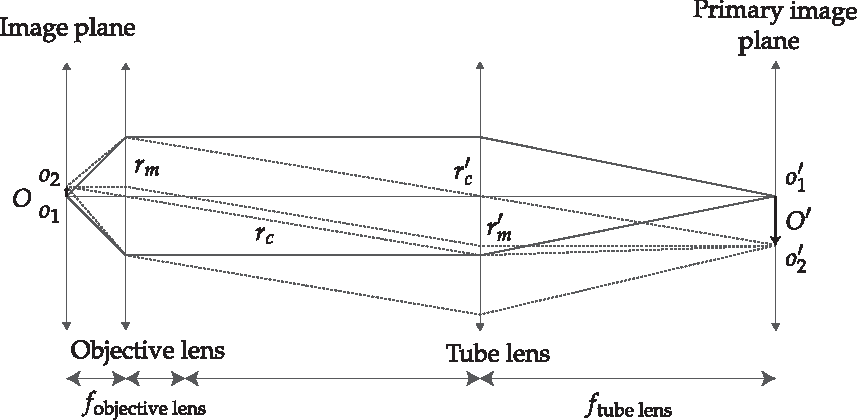
\includegraphics{./magnification}
    \caption{Ray diagram of a two lens magnification system, with a \gls{4f} configuration.}
    \label{fig:magnification}
\end{figure}

% Tube lens may also be used to correct for image abberations

%Great advantage is that the lgiht path behind the objective only contains paralel light, means can add optical elements without distortions the beam path.

% Other adsvantage is you can focus by moving the \gls{objective lens}

%and the overall magnification of the

%\subsubsection{Magnification}

\subsubsection{Field of view}

\index{field of view}

The observable objective \gls{FOV} is limited by the aperture stop of the system typified as the field number (\(F_\text{n}  \)) and the \gls{objective lens} magnification \(M_{\text{objective}} \):
%The maximum field of view (\(F_{n} \))available is by :

\begin{align}
    \gls{FOV} = \frac{F_{n}}{M_{\text{objective}}}
\end{align}

The field number achievable in a real \gls{objective lens} design is limited by the image degradation caused through optical aberrations.
Modern objective technology can reach up to \SI{28}{\milli\meter} from the previous standard of \SI{20}{\milli\meter}.

\subsubsection{Illumination}

The illumination system defines the contrast mode, the resolution of the instrument, and the overall brightness.
Two principally different optical setups are in use in optical microscopes.
The optically simpler of the two is the source focus or critical illumination and the other, which is by far more prevalent, is called Köhler illumination.

Critical illumination uses a single \emph{condenser} lens whereas Kohler illumination uses an additional \emph{collector} lens.
The use of two illumination lenses allows for a conjugate \gls{4f}  system of illumination to the detection optics, this ensures that all ray bundles passing through the sample are parallel and the illumination brightness is homogenous.
Having a conjugated illumination also allows for alternative contrast methods to be implemented.

In the illumination beam paths discussed earlier, the specimen is placed between the light source and the \gls{objective lens}.
In many cases, however, it is advantageous to illuminate the specimen from the side of observation (\emph{epi-illumnination}).
For instance, when looking at the reflection of opaque samples, or the emission of fluorescent samples.
Optically the illumination is the same or similar with the condenser lens then being the imaging \gls{objective lens} as well.
% In that case, some optical components of illumination and imaging are identical, for example, the \gls{objective lens}.

\subsection{Resolution}\label{sec:resolution}\index{resolution}
%Magification versus resolution

Resolution refers to the fineness of detail that can be recognised in an image, such as small and intricate structures or the distance between closely placed small objects.
The latter case, specifically the smallest separation at which two point-like emitters produce an image that can be distinguished as coming from two sources, is used to define and quantify the optical resolution.
% Using light microscopy
% Using light microscopy, minute objects can be discriminated from each other when they are positioned at a minimum distance of -0.25 mum from each other and green light and a high-quality oil-immersion \gls{objective lens} are used.
% This obviously means that proteins and supramolecular complexes occurring in living cells cannot be recognized in detail.
% In later chapters, we discuss how the principal optical resolution limit can be overcome or circumvented by advanced optical techniques.

\subsubsection{Angular aperture and numerical aperture}\index{numerical aperture}

%An \gls{objective lens}es is limited by
The maximum half acceptance angle (\gls{alpha}) of an \gls{objective lens} limits the amount of light that can be collected from the sample.
It is the half angle of the cone at the optical centre of the objective lens, outside of which light is not collected for imaging.
An \gls{objective lens} may be approximated to applying a Fourier transform of the imaging space, through an aperture with radius \(a\) with an imaging plane at the far field.
This leads to high frequency information being omitted during the imaging process and the lens behaving as a low-pass filter for optical frequencies.
The electric field (\gls{E}\((r)\)) and resultant intensity (\gls{I}\((r)\)) distribution of a single point (delta function) at the primary image plane then becomes:

\begin{align}
    E(r) &\propto E_0 \frac{J_1 \left( \frac{2\pi r}{\lambda}\sin \alpha \right)}{ \frac{2\pi r}{\lambda} \sin {\alpha})}\label{eq:E_airy}\\
    \implies
    I(r) &= I_0 \left[\frac{J_1 \left( \frac{2\pi r}{\lambda} \sin \alpha \right)}{ \frac{2\pi r}{\lambda} \sin {\alpha})}\right]^2\label{eq:I_airy}
\end{align}

Where \gls{J_1} is a Bessel function of the first kind and \gls{alpha} is the half opening angle of the objective lens.
This function is more commonly known as an \Gls{airy disk} as shown in \figurename~\ref{fig:airy_disk}.

\begin{figure}
    \centering
    \begin{subfigure}[b]{\textwidth}
        %\centering
        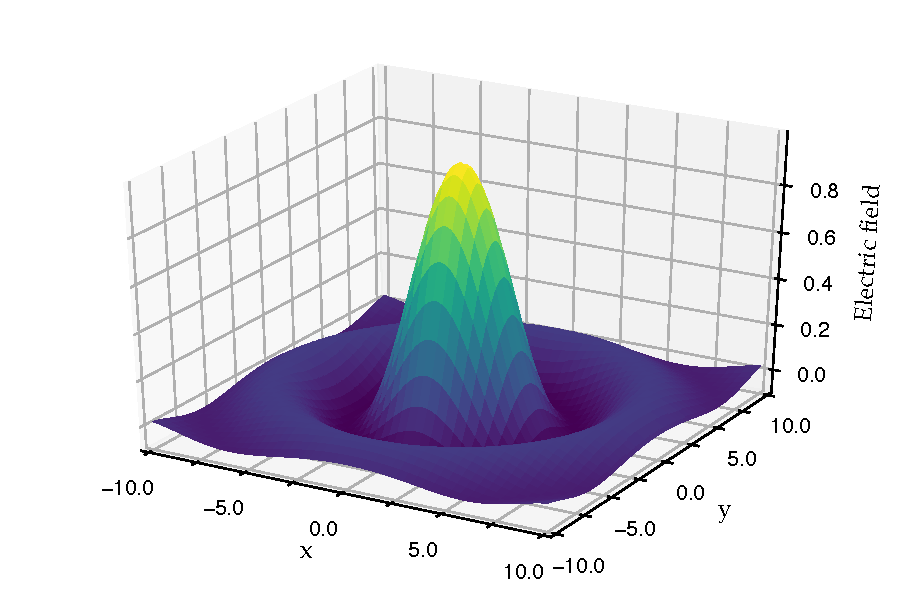
\includegraphics{+airy_E_fill}
        \caption{\(E(r)\), equation~\eqref{eq:E_airy}}\label{fig:airy_E_fill}
    \end{subfigure}\quad
    \begin{subfigure}[b]{\textwidth}
        %\centering
        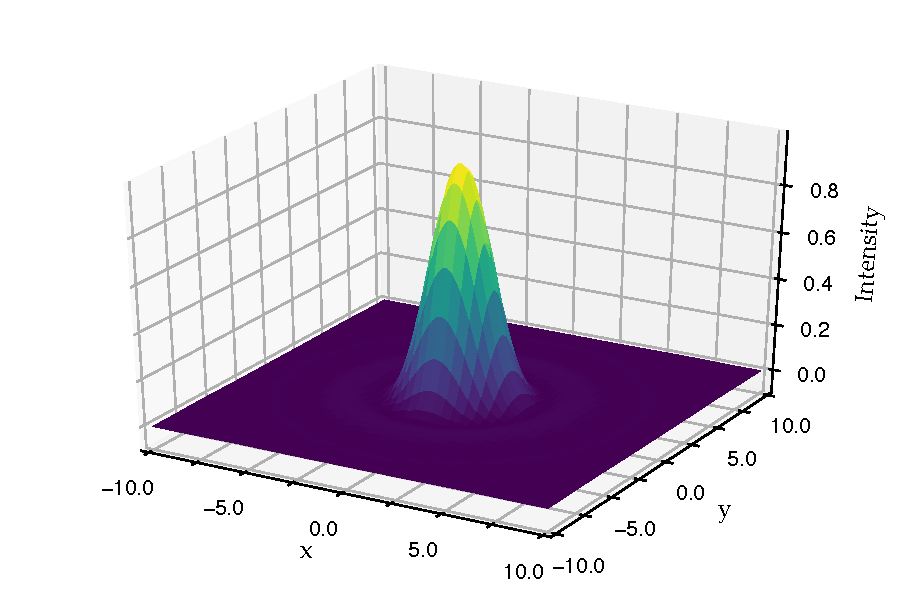
\includegraphics{+airy_I_fill}
        \caption{\(I(r)\), equation~\eqref{eq:I_airy}}\label{fig:airy_I_fill}
    \end{subfigure}
    \caption[Electric and intensity amplitudes of a theoretical \gls{airy disk}]{Electric and intensity amplitudes of a theoretical \gls{airy disk}, lateral distances \(x\) and \(y\) are given in units of \(\frac{2\pi r }{\lambda}\sin {\alpha}\)}\label{fig:airy_disk}
\end{figure}

\subsubsection{Lateral resolution}

Point emitters are therefore imaged more faithfully with wider collecting angles and with shorter wavelength light.
By placing two point emitters close such that the first zero crossing of the Bessel function \gls{J_1} coincides with the centre of the second point emitter gives a distance of:

\begin{align}
    r_{0,\text{objective}} &\approx \frac{0.61\lambda}{n\sin\alpha} = d_r \label{eq:lateral_res}\\
    \implies d_r &= \frac{1.22 \lambda}{NA_{\text{objective}}}
\end{align}

The resulting distance is Rayleigh's criterion for resolution which provides a limit to the resolution of a system based on a dip in intensity maxima, between two neighbouring emitters, of \SI{75}{\percent} as shown in \figurename~\ref{fig:airy_rayleigh}.

%Coherent and incoherent
\subsubsection{Axial resolution}

The \Gls{airy disk} describes the in-plane lateral intensity distribution, with an analogous analytical function propagating axially.
Once again, by comparing the the distance to the first zero in intensity along \(z\) an analytical definition can be formed:

\begin{align}
    z_{0,\text{objective}} = \frac{2n\lambda}{{NA}^2} \label{eq:axial_res} = \frac{1}{2} D_{\text{objective}}
\end{align}

The achievable axial resolution is governed by axial extension of the \gls{PSF} which is \(2z_{0,\text{objective}}\) and is commonly called the \emph{\gls{depth of field}} (\(D_{\text{objective}}\)).
The \gls{depth of field} physically refers to the distance a focussed object may be moved axially before losing image fidelity to defocus.

\begin{figure}
    \centering
    \begin{subfigure}[b]{\textwidth}
        \centering
        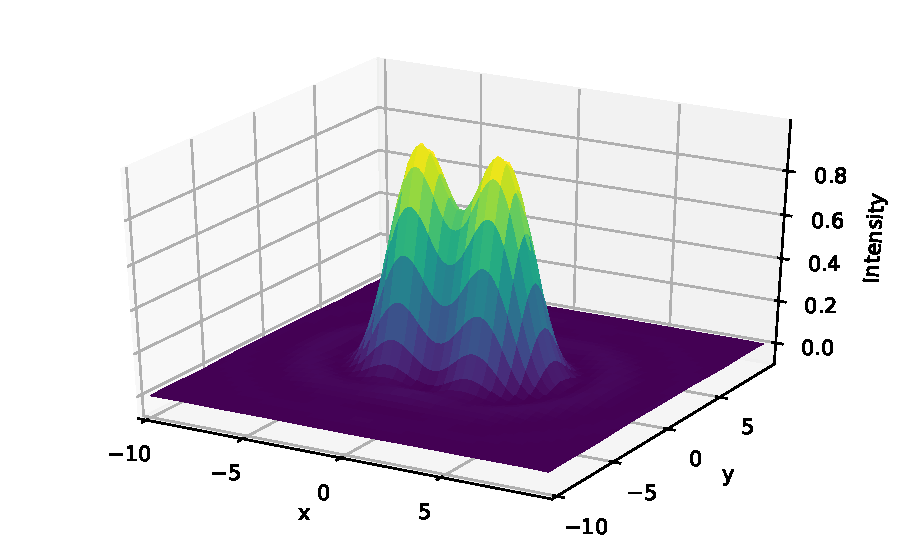
\includegraphics{+airy_rayleigh}
        \caption{The Rayleigh criteon, whereby the centre of the second emitter sits at the first zero of the first emitter.}\label{fig:airy_rayleigh}
    \end{subfigure}
    \begin{subfigure}[b]{\textwidth}
        %\centering
        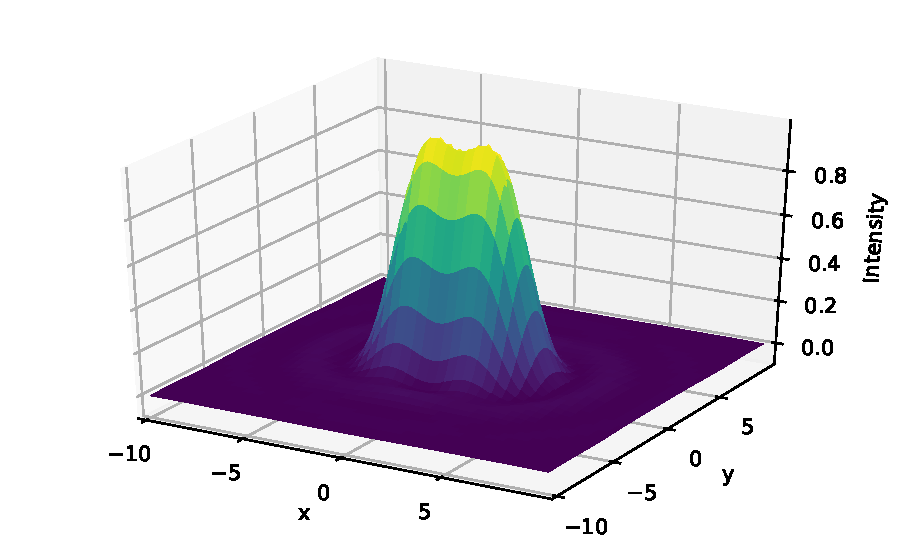
\includegraphics{+airy_sparrow}
        \caption{The Sparrow criteon, whereby the centre of the second emitter is one \gls{FWHM} of the function distant from the first emitter.}\label{fig:airy_sparrow}
    \end{subfigure}
    \end{figure}
    \begin{figure}
\ContinuedFloat\begin{subfigure}[b]{\textwidth}
        %\centering
        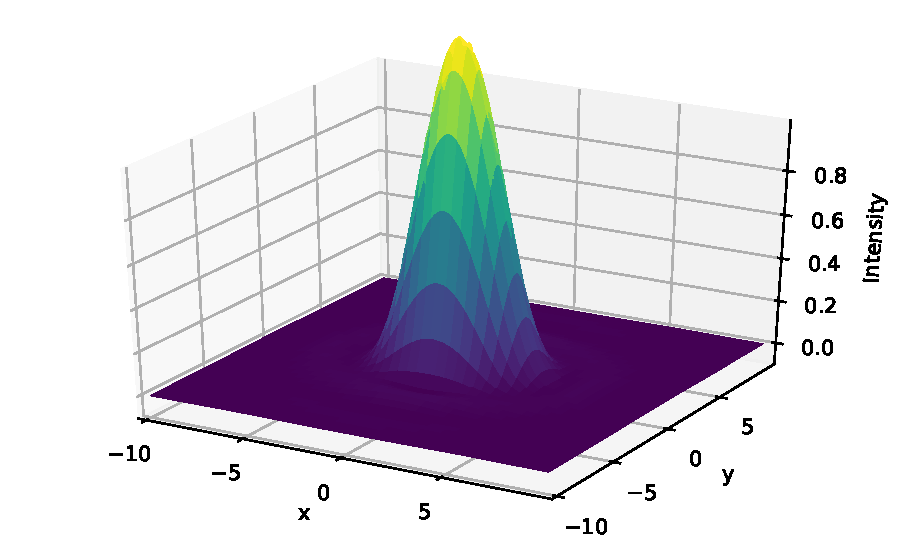
\includegraphics{+airy_too_close}
        \caption{Unresolved, depicted here as being half the Sparrow limit}\label{fig:airy_too_close}
    \end{subfigure}
    \caption[Resolution criterion]{The resolution of a system is governed by the resolving capability of two nearby point emitters.
    (\subref{fig:airy_rayleigh}) and (\subref{fig:airy_sparrow}) show the Rayleigh and Sparrow criterions respectively with (\subref{fig:airy_too_close}) showing point emitters too near to be resolved due to the lack of any intensity contrast between them}\label{fig:airy_disk_resolution}.
\end{figure}

% Depth of field
%
% \subsubsection{Depth of field}

\subsubsection{Sampling}

% \index{Nyquist sampling}

Once transmitted, the irradiance image produced in the primary image plane is typically recorded digitally, using using a \gls{CCD} array sensor or similar device (e.g.~an \gls{sCMOS} array).
According to \Gls{nyquist sampling theory}, the resolution of the detector (i.e.~the pitch separating the adjacent rows of sensor elements, \gls{photosite}s) required to resample the image information faithfully is \(d_\text{detector} = \frac{d_r}{2}\).
To then choose the correct system magnification (\(M_\text{system}\)) it follows that:

\begin{align}
    M_\text{system} = \frac{2d_\text{detector}}{d_r}
\end{align}

For a detector with \gls{photosite}s (detector pixels) in a square array with a pitch of \SI{6}{\micro\meter}, a magnification on the order of \(50\times \) is sufficient for diffraction limited imaging using visible light.\index{magnification}
Magnification in excess of this limit is deemed \emph{empty magnification} and decreases the overall \gls{SNR} of the recorded image.
However, such over-sampling plays an important role in super-resolved systems where the additional pixel information, though diffraction limited, may be used to increase resolution computationally~\cite{betzigImagingIntracellularFluorescent2006}.
\pagebreak
\begin{figure}
    \centering
    \begin{subfigure}[b]{\textwidth}
        \centering
        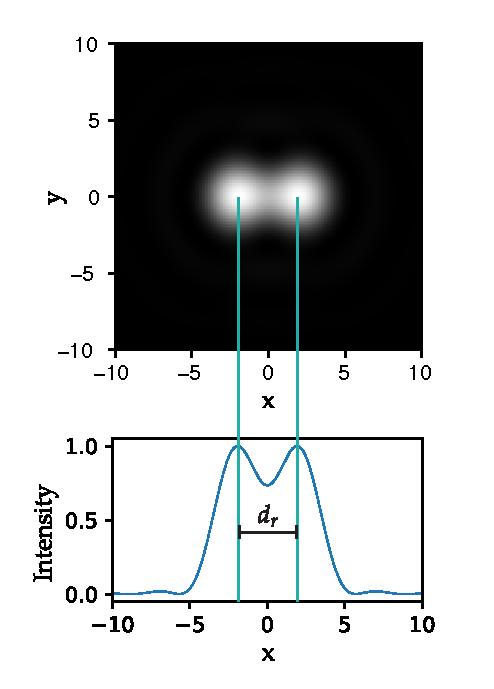
\includegraphics{./sampling/sample_master}
        \caption{Intensity image of a pair of resolved point emitters separated by the Rayleigh distance \(d_{r} \), where \(x \) is lateral distance in units of \(\frac{2\pi r }{\lambda}\sin {\alpha} \) and intensity quantifies irradiance (\SI{}{\watt\per\meter\square} in the primary image plane.)}\label{fig:sample_master}
    \end{subfigure}
\end{figure}
\begin{figure}
\ContinuedFloat\centering
      \begin{subfigure}[t]{0.4\textwidth}
        \centering
        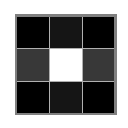
\includegraphics[width=0.9\textwidth]{./sampling/digital_airy_sample_3}
        \caption{Sampled using 3 by 3 pixels\\
        \(d_{\text{detector}} = 1.5 \times d_{r}M_{\text{system}}\)}\label{fig:digital_airy_sample_3}
    \end{subfigure}\quad
    \begin{subfigure}[t]{0.4\textwidth}
        \centering
        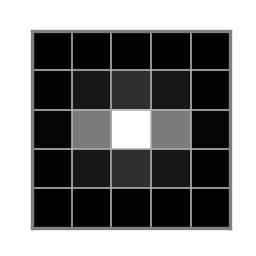
\includegraphics[width=0.9\textwidth]{./sampling/digital_airy_sample_5}
        \caption{Sampled using 5 by 5 pixels\\
        \(d_{\text{detector}} = 0.9 \times  d_{r}M_{\text{system}}\)}\label{fig:digital_airy_sample_5}
    \end{subfigure}\\
    \begin{subfigure}[t]{0.4\textwidth}
        \centering
        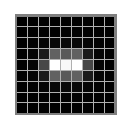
\includegraphics[width=0.9\textwidth]{./sampling/digital_airy_sample_9}
        \caption{Sampled using 9 by 9 pixels\\
        \(d_{\text{detector}} = 0.5 \times d_{r}M_{\text{system}}\)}\label{fig:digital_airy_sample_9}
    \end{subfigure}\quad
    \begin{subfigure}[t]{0.4\textwidth}
        \centering
        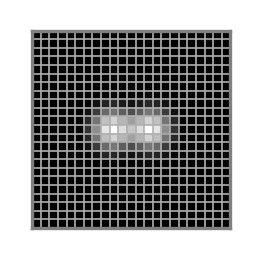
\includegraphics[width=0.9\textwidth]{./sampling/digital_airy_sample_23}
        \caption{Sampled using 23 by 23 pixels\\
        \(d_{\text{detector}} = 0.19 \times d_{r}M_{\text{system}}\)}\label{fig:digital_airy_sample_23}
    \end{subfigure}\\
    \begin{subfigure}[t]{\textwidth}
      \vspace{\abovecaptionskip}
      \centering
      
\includegraphics{./sampling/colourbar}\\
      Irradiance in primary image plane
    \end{subfigure}
    % \begin{subfigure}[t]{0.1\textwidth}
    %     \centering
    %     
\includegraphics{./sampling/colourbar}
    %     % \caption{Sampled using 23 by 23 pixels\\\(d_{\text{detector}} = 0.19 \times d_{r}M_{\text{system}}\)}
    %     % \label{fig:digital_airy_sample_23}
    % \end{subfigure}
    \caption[The effect of sampling on a \gls{PSF}]{The effect of sampling on a \gls{PSF}.
    Point emitters in (\subref{fig:sample_master}) are sampled by a detector with varying detector pixel widths relative to the optical resolution of the system.
    % analogous to varying magnification.
    (\subref{fig:digital_airy_sample_9}), shows Nyquist sampling;
    (\subref{fig:digital_airy_sample_23}) is over sampled, giving super detector resolution.
    (\subref{fig:digital_airy_sample_3}) and (\subref{fig:digital_airy_sample_5}) do not preserve resolution as they are below Nyquist sampling and the images may be mis-interpretted as being produced by a single emitter or by a continuous feature, instead of two distinct point emitters and hence detect a single emitter.}\label{fig:digital_airy}
\end{figure}
\pagebreak

% \subsubsection{Light collection efficiency}
%
% To calculate the the collecting efficiency of a lens, a single radiating source is considered, a Lambert radiator.
% The flux collected is proportional to the spherical segment carved out by the lens.


\section{Fluorescence microscopy}
\subsection{Contrast in optical microscopy}
% Phase contrast, dark field
\subsection{Fluorescence}\index{fluorescence}

Fluorescent molecules absorb photons of a particular energy with an excitation wavelength (\(\lambda \)) (where energy \(= h \nu = h \frac{c}{\lambda}\)), a short time later the molecules re-emit a photon with lower energy, this energy difference gives rise to a red-shift of the emitted photon.
This shift in colour allows for suitably coated glass to chromatically separate the desired fluorescent signal and the undesired scattered incident light.
% Upon being exciting by incident light, an electron within a fluorescent molecule may excite to a higher energy level, provided it has sufficient potential energy to traverse the energy barrier.
Upon being exciting by incident light, a fluorescent species may be transformed to a higher level state.
The occurs when an electron in the ground state energy level absorbs an incident photon with an energy greater than the difference of the exited state (\(S_1\)) and the ground state (\(S_0\))
Once in the higher excited state (\(S_1\)), \gls{fluorophore}s will exist there for an average lifetime (\gls{tau}), slowly losing energy to the surroundings through vibrations and molecular collisions.
Once the electron has \emph{trickled} down the energy levels, it will return to the ground state (\(S_0 \)) emitting a photon with an energy less the amount of energy lost when in the excited state, the \emph{\Gls{stokes shift}}.
Electrons may also return to the ground state through molecular collisions or an \emph{intersystem} crossing whereby the electron finds a path via transient states with lower energy requirements, such as the \emph{triplet state}.
See \figurename~\ref{fig:jablonski_triplet_new}

%\subsubsection{Fluoresence spectra}
In practice, multiple (split) energy levels slightly above the ground and excited states tend to promote a distribution of multiple different emission wavelengths.
Fluorescent molecules therefore have broad excitation and emission spectra rather than discrete excitation and emission lines, see \figurename~\ref{fig:fluo_spectra} for typical fluorescent molecules used in microscopy.

An important advantage of fluorescence microscopy is labelling \emph{\gls{specificity}}, which refers to the ability to accurately label markers, features or molecules within a specimen.
Multiple labels in different spectral windows can further elucidate how labelled entities interact within the sample.

\begin{figure}
    \centering
    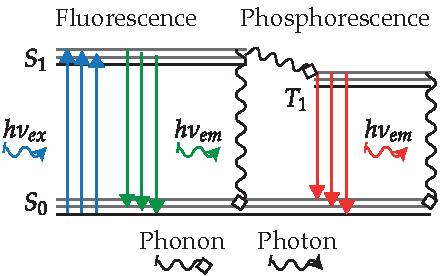
\includegraphics{jablonski_triplet_newer}
    \caption[Standard jablonski diagram]{
    Jablonski diagram representing a green fluorescent molecule.
    Transitions are indicated as excitation (\emph{ex}) or emission (\emph{em}). %represented by waving vectors.
    Species in state \(S_0 \) receive energy from blue incident light,
    this causes the electrons to transition to state \(S_1 \).
    From \(S_1 \) species may lose energy non-radiatively and re-emit a greener photon when relaxing back to \(S_0 \).
    Once in \(S_1 \) electrons may transition to a triplet state, re-emitting a photon through phosphorescence.
    A molecule in a triplet state will be for a longer time to \(S_1 \) and with an increased chance of oxidation which causes photobleaching.%risk photobleaching through oxidation
    }\label{fig:jablonski_triplet_new}
\end{figure}
%\subsubsection{Specificity}


\subsubsection{Labelling}\index{labelling}

% Labelling of sites direct, primary and secondary.
Fluorescent labels may be attached to a site on a molecule directly, using primary antibodies or secondary antibodies.
Direct immunolabeling involves attaching an antibody to the target molecule directly and having the dye molecule attach to another site on the antibody.
Indirect immunolabeling labelling attaches a secondary antibody to the primary antibody and attaches a fluorescent dye to the secondary.
Indirect immunolabeling labelling has the advantage of ease of labelling for most target molecules with most dye molecules.
However, effective resolution (which is distinct from imaging resolution in that effective resolution refers to locating target species) is lost due to the longer ligand attaching to the target.%, but for convenience of dyes with the suitable anti-group being available.
% Ligand length is also dependant of the type of staining, direct or secondary.
% Direct labels refer to the dye directly binding to an active site on the molecule of interest,
The staining process is further inhibited by cellular mechanics; a cell may not take up (endocytose) the stain or be it may degraded by the cell (through \gls{autophagy} in the \gls{lysosome}).

For non-membrane permeable dyes, \gls{transfection} techniques, though invasive, do exist~\cite{kimMammalianCellTransfection2010}.
Staining can also lead to non-specific binding of fluorescent molecules reducing confidence in specificity and increasing the overall background fluorescent signal in-turn decreasing the image contrast.

For live organism imaging, staining is impractical.
Genetic manipulation can allow for fluorescent proteins to be expressed with high specificity as the cells themselves are producing the desired \gls{fluorophore}, covalently bonded to the target molecule; with good spatial homogeneity when compared to soaking samples in dye; and low sample toxicity.

%TODO Talk about auto Fluoresence

%NC :

% Can you put a brief section here on filter sets? This wopuld make your jump from talking about lasers to detectors less jarring.
%
% I think you also need a short paragraph summarising what people usually do (most people use lasers for point scanning and super res due to the high intensity for multiple colour microscopy people usually combine lasers these wavelength are most comon. NThen talk about spectral selection.
%
% Lasers are combined using dichroic mirrors then snt to the sample a dichroic seperates the excitation and emission into different paths and emission filters further suppres out of band signal. An example excitation laser and filter set for 3 colour imaging is shown in figure..

%\subsubsection{Image contrast}
%\subsubsection{Specificity}
\subsection{Fluoresence microscopy}

\subsubsection{Illumnination}

%The Merucry Arc lamp is unibiqitous in lamp-based fluorsence mciroscopes.
The mercury arc lamp became the ubiquitous excitation source for fluorescence microscopy because it emits a broad visible emission spectrum at a higher intensity than a standard halogen lamp.
However, advances in \gls{LED} and \gls{Laser} technology have caused a technological shift towards these alternative sources especially in fluroesence microscopy where narrow spectrum excitation light sources are desirable.
Modern \gls{LED}s and \gls{Laser}s are now have the the stability and intensity to compete with lamp based sources, with more available intensity and homogeneity.

\gls{LED} sources are currently behind Lasers in terms of the intensity required for certain imaging applications due to the \emph{\gls{etendue}} (or geometric extent defined as the product solid angle of of the system's entrance pupil and the area which is conserved through optical systems) of the emission.
As \gls{etendue} is preserved through any system of optics an \gls{LED} source, having large \gls{etendue}, will be very photon inefficient, to the point of being infeasible for applications such as point-scanning.

\Gls{Laser}s are generally limited to very specific excitation lines due to the materials used, particularly in the case of diode lasers.
\Gls{Laser} light sources are also optically \gls{coherent} which causes self-interference in the illumination profile (speckle) and the sample.
%For wide-field imaging LED sources may be sufficient with an added benefit of being incoherent.
%Emission wavelengths are selected from lamp and white LED sources using emission filters.
A \gls{super-continuum laser} sources uses non-linear optical effects, typically induced within a long photonic crystal fibre, to produce broad-spectrum visible \gls{Laser} light.
From this spectrum, wavelengths may then be selected using emission filters, as with lamp-based sources and white LED sources.
This is in contrast to systems with monochromatic lasers as adding more laser lines requires the physical addition of a new laser, making \gls{super-continuum laser}s versatile.
% The downside being that t
However, the intensity of the of the pump laser source is spread into the entire spectrum causing narrow selected emission bands to have relatively low intensities.
% To add additional emission lines into a system with monochromatic lasers requires adding more laser lines physically, this approach is desirable for making systems versatile.
% The downside being that the intensity of the of the pump laser source is spread into the entire spectrum causing narrow selected emission bands to have relatively low intensities.

\begin{figure}
    \centering
    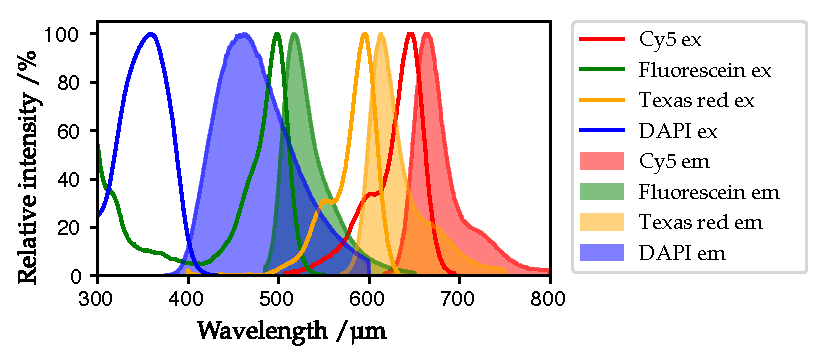
\includegraphics{./fluorphores/++multi_plot.pdf}
    \caption[Common fluorescence excitation spectra]{Fluorescence excitation (lines) and emission (filled curves) spectra of the compounds Fluorescein, Texas red, Cy5 (all homocyclic) and DAPI.}\label{fig:fluo_spectra}\index{fluorescence spectra}
\end{figure}

\subsection{Signal collection}

Once created, the detected image is recorded for analysis and dissemination.
%Modern camera technology
Sensors made up of digital \gls{pixel} (\gls{photosite}) arrays are used in \gls{wide-field} fluoresce microscopes (e.g. \gls{CMOS} and \gls{CCD}) and photo-multiplier tubes (PMT) are used in most laser scanning microscopy.

\subsubsection{Detectors}\index{detectors}

Modern \gls{wide-field} detectors come in many types, all of which exploit semi-conductor physics to convert incident photons into electrons.
\Gls{CCD} based detectors collect electrons during an exposure and transfer in a serial manner through conversion electronics to create digital images, as depicted in \figurename~\ref{fig:sensor_chips}.
\Gls{ICCD} detectors follow the same protocol but use on-photo-site electron cascading to increase the signal and \emph{intensify} the read image.
\gls{EMCCD} detectors transfer their entire frame to a separate conjugate chip which digitises the image for computation.
As the frame is being transferred the signal is amplified to multiply electrons collected in the conjugate digitisation site and intensify the image as in \gls{ICCD}.
Transferring the entire frame reduces the digitalisation time and increase the imaging frame-rate.

\gls{CMOS} chips directly convert radiant exposure to a digital value on a per pixel basis.
The additional circuity found off-chip in \gls{CCD} detectors is embedded in each pixel.
Though this reduces the overall fill factor feasible in each chip, this can be recovered using a micro-lens array to focus directly onto the active read area of the \gls{photosite}.
The per-photo-site architecture allows for a region-of-interest area to be addressed.
\gls{CMOS} detectors made specifically to address quantitative scientific (\gls{sCMOS}) usage tend to have: small pixel sizes; low read noise; large detection arrays; large dynamic range and no multiplicative noise~\cite{verveerAdvancedFluorescenceMicroscopy2015}.

%\subsubsection{Single molecule detection}

\subsubsection{Sensor model}

Each measured pixel value in the digital image, \(y_i\), is therefore modelled as follows, where \(t_\text{exp}\) is the exposure time, \(g\) is the gain, \(a_i\) a per-pixel factor to allow for non-uniform response to illumination (often assumed constant is unity) and \(f_i\) the incident radiant flux on the photo-site. The numbers of the photo-electronics collected at the photo-site is Poisson-distributed, with expected value:
\begin{align}
  E(e_i) = t_\text{exp} a_i f_i
  \intertext{The recorded pixel value is affect by sensor gain and fixed readout noise:}
  y_i = g(a_i) + r_i(g)
  \intertext{\(f_i\) (irradiance) can be quantified from \(\mathbf{y}\) by taking a bias frame \(\mathbf{b}\) and estimate:}
  \hat{f_i} = \frac{y_i-b_i}{g t_\text{exp} a_i}
\end{align}

\subsubsection{Noise}\index{detector noise}

Adverse noise arises in optical microscopes from several compounding effects.
The larger the noise level the lower the \gls{SNR} and the more degraded the recorded image will be.

The \emph{\gls{dark current}} (noise) contribution occurs in the detectors themselves as the semiconductor material produces erroneous electrons from converting thermal phonons.
\Gls{dark current} increases linearly with integration time and so chip cooling is recommended.
\emph{\Gls{photon noise}} (shot) originates from corpuscular photons arriving at the detector following a temporal \Gls{poissonian distribution}.
An image containing \(n \) photons will suffer a variation of \(\sqrt{n} \) in photons being emitted, this can appear as valid structure once recorded.
\emph{\Gls{read noise}} is rooted in the conversion process of the analogue voltage of electrons, at each \gls{pixel}, to digital values.
The intensity response across a detector may also be inhomogeneous, this may be flat-field corrected using a calibration from a uniform intensity source.
\footnote{manufacturers for \gls{sCMOS} cameras apply this correction as standard}

A detector with a large \emph{\gls{quantum efficiency}} (photon to electron conversion efficiency), will be able to overcome noise more quickly.
The \emph{\gls{dynamic range}} of the detector is the intensity range at which the weak fluorescent signal can be recorded above background noise.
The \emph{\gls{bit depth}} (8 or \SI{16}{\bit} typically) of the detector defines the detectable intensity resolution, which is of particular use for very weak signals.
Increasing the integration (exposure) time of the detector will bring the desired signal out of random background noise.
However this can be limited by other effects such as sample movement on the timescale of imaging or photobleaching.
%NC
%Close with noise is one factor which limits fluorescence microscopy.
% One way of reduceing the effects of noise is to increase exposure time or excitation intensitty. However this can be limited by other effects such as sample movement on the timescale of imaging or photobleaching (start next section0

\begin{figure}
    \centering
    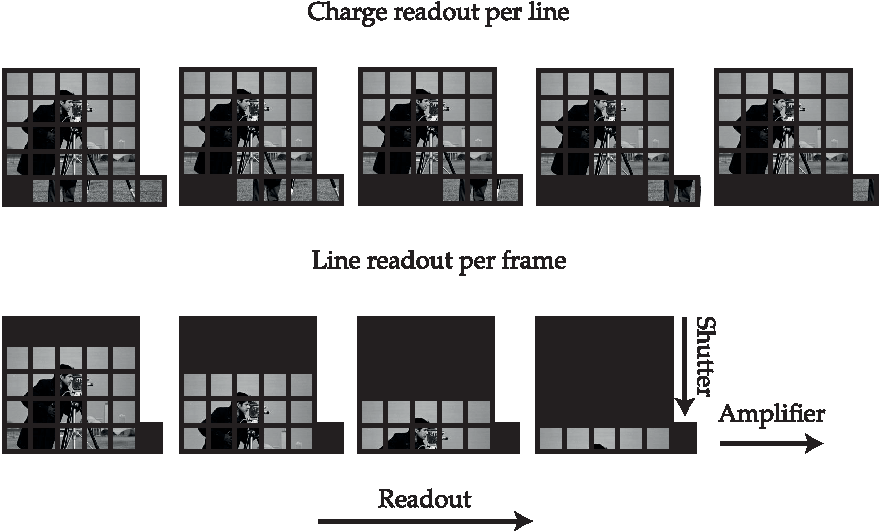
\includegraphics{./sensor_chips}
    \caption[Schematic of how electronic charge is transferred from a \gls{CCD} array through an amplifier]{Schematic of how electronic charge is transferred from a \gls{CCD} array through an amplifier.
    \textbf{Charge readout per line:} charge is serially transferred along the line being read into a single amplifier.
    \textbf{Line readout per frame:} once the line is read, the entire frame is shifted down to be read, acting as a shutter.
    Serial reading through a single amplifier is slow.}\label{fig:sensor_chips}
\end{figure}


% \begin{figure}
%     \centering
%     
\includegraphics{./imaging_sensors.pdf}
%     \caption{Imaging sensors}
%     \label{fig:imaging_sensors}
% \end{figure}

\subsection{Limits of fluorescence microscopy}

\subsubsection{Photobleaching}

Fluorescently stained samples will slowly fade in radiance (under fixed illumination) over time as the dye molecules are photochemically destroyed through photobleaching.
The process occurs typically through photo-oxidation, once the \gls{fluorophore} is in an excited state it may then energetically fall into a triplet state where it is more likely to permanently bond with oxygen radicals.
Dye medium can be buffered with scavengers of oxygen radicals to mitigate the process of bleaching.
In some \emph{in vivo} experiments, genetically modified organisms suffer less from photobleaching as molecules that have photo-bleached are continually replaced by newly expressed (transcribed) \gls{fluorophore}s.

%Whilst this is true I feel like the firsat half of the sentence is jarring.
% When imaging live samples expressing fluorescent proteins photobleached molecules can be replaced by newly transcribed(?) fluorescent proteins

\Gls{photobleaching} can be exploited to learn about a specimen, using \gls{FRAP}; wherein an imaging region is purposefully bleached, so that the rate of diffusion of unbleached dye molecules into the \gls{FOV} can be estimate.
The rate of return of intensity in the imaging region then gives a measure of diffusion.

% FRET STORM PALM
%Some molecules have the valuable property of being able to reverse

%\paragraph{Reversible photobleaching}
\subsubsection{Phototoxicity}

Fluorescent dyes can act as \gls{photosensitier} during live imaging, resulting in damage to functionality of the cell.
%What about other autofluorescent molecules in the sample and other absorbances? I think you need to mention this as one of the niches of light sheet is that it reduces light does, so make it clear just how bad too much light is
Chromophores of fluorescent proteins are shielded by direct contact from molecular oxygen through protein moiety, and so fluorescent proteins may be less phototoxic to living specimens~\cite{pawleyHandbookBiologicalConfocal2006}.
% It has beeen suggested that acceptable levels of light exposure will be on the order of a solar.
%Direct and intense light exposure


%Photodynamic effwect
%Intensity induced
%\subsection{Resolution}
\section{Three dimensional fluorescence microscopy}

The light microscope as discussed is inadequate for imaging thick three dimensional samples as light from the sample, above and below the focal plane, contributes to the detected light.

\subsection{Confocal microscopy}

Marvin Minsky proposed the first \gls{confocal microscope} in the late 1950s to image deep into brain tissue.
A pinhole is placed in a conjugate image plane in the detection path which precludes out-of-focus light from being detected.
The narrower the pinhole the better the optical sectioning, though sacrificing the received signal.

In Minsky's microscope the sample was mechanically scanned to build a volumetric image.
By mechanical scanning, the imaging speed is greatly reduced due to the speed of responses of the stage, the maximum speed of travel of the stage and the relaxation time of the stage.
Specimens are prone to spatial shifts during scanning as well, which causes distortions in the final image.

Modern \gls{confocal microscope}s use often \gls{galvanometric scanning mirrors} to sweep a laser beam through the sample to build an image.
Though faster than mechanical scanning, video-rate scanning confocal microscopy is only viable using \gls{resonant scanning mirrors} and high power lasers (due to the photon rejecting nature of the confocal pinhole).

% \subsubsection{Spinning disk confocal microscopy}
%
% The speed of Single point confocal microscopy can be greatly improved by producing multiple points.

%\subsubsection{Principles}
%\paragraph{Spinning disk confocal microscopy}
\subsection{Two photon (2P) microscopy}\label{sec:2p}

% 2P microscopy is a part of a breed of techniques called non-linear microscopes which exploit the quantum nature of fluorophores.
% 2P imaging provides the most efficient signal generation.

The photon rejecting pin-hole of \gls{confocal microscope}s can be entirely avoided by using infra-red laser sources.
Exciting a \gls{fluorophore} to an excited state requires a quantised amount of energy, which is typically supplied by a single photon.
However, two photons, each with double the desired wavelength, also contain the requisite amount of energy to cause the same excitation.
For this event to occur, there needs to be a high photon density surrounding the \gls{fluorophore}.
In a laser scanning system, this means that the beam focus of the \gls{objective lens} is the most likely place for fluorescence to occur, with a sharp decline in intensity axially, providing optical sectioning.

By using \gls{2P} excitation, greater depth imaging (\SI{\sim6}{fold} deeper) can be achieved with reduced \gls{photo-toxicity}, making the technique very useful for non-invasive live imaging.

\subsubsection{Drawbacks} %500nm -> 10^-01.4 10^+1.8

Water, which is abundant in biological specimens, has a large absorbance in the infrared spectrum, 3 orders of magnitude larger than in the visible spectrum (e.g. \SI{532}{\nano\meter} versus \SI{1064}{\nano\meter});
combined with the high energy needed to create the \gls{2P} effect at the focal point, this can cause localised heating which can in-turn be damaging to specimens and cause optical \gls{aberration}s.
Localised heating can be mitigated by moving the beam sufficiently quickly such that significant heating does not occur.
Using infrared excitation also means that the \gls{2P} imaging has a coarser lateral resolution when compared to visible confocal microscopy due to their wavelength (Equation~\eqref{eq:lateral_res}).
Finally, infrared-red laser sources are more difficult to work with for alignment than visible \gls{Laser}s.
% prohibitively expensive and, until recently, reliable turn-key solutions were not viable.

\subsection{Structured illumination microscopy}\label{sec:SIM_theory}

In \gls{SIM}, the sample is sequentially illuminated with several periodic patterns using a fast \gls{wide-field} microscope.
The mixing of each illumination pattern with the structure of the fluorescent sample results in several diffraction limited images from which a high-resolution image of the original sample can be computationally reconstructed.
Furthermore optical sectioning can also be achieved using specific illumination.
% means that additional resolution can be extracted both in \(xy \) and \(z \).

\begin{figure}
    \centering
    % \hfill
    \begin{subfigure}[t]{0.25\textwidth}
        \centering
        
\includegraphics[height=3cm]{./sim/otf}
        \caption{\Gls{wide-field} \gls{OTF}}\label{fig:sim_otf}
    \end{subfigure}\hfill
    \begin{subfigure}[t]{0.25\textwidth}
        \centering
        
\includegraphics[height=3cm]{./sim/third_flower}
        \caption{\gls{SIM} image reconstructed for one orientation with a \gls{super-resolution} improvement in \(k_y \)}\label{fig:sim_third_flower}
    \end{subfigure}\hfill
    \begin{subfigure}[t]{0.35\textwidth}
        \centering
        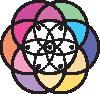
\includegraphics[height=3cm]{./sim/full_flower_alt}
        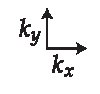
\includegraphics{./sim/xy_coordinates}%\label{fig:sim_coordinates}
        \caption{\gls{SIM} image reconstructed for three orientations, near homogenous 2D \gls{super-resolution} improvement}\label{fig:sim_full_flower}
    \end{subfigure}
    % \begin{subfigure}[t]{0.11\textwidth}
    %     \centering
    %     % \caption{Sim full flower}
    % \end{subfigure}
    % \hfill
    \caption[Schematic of \gls{SIM} reconustruction in Fourier space]
        {Schematic of \gls{SIM} reconustruction in Fourier space.
        In (\subref{fig:sim_otf}), the circular area corresponds to the passband of the \gls{objective lens}, the edge being the frequency cut-off.
        The raw data in (\subref{fig:sim_otf}) consists of superposed original image information
        positioned at three different origins.
        Once delineated, the high-resolution information can be relocated to the correct position, resulting in a wider pass-band, (\subref{fig:sim_third_flower}).
        The process is repeated three times to isotropically fill the available frequency space by rotating the illumination patterns, (\subref{fig:sim_full_flower}).
        }\label{fig:sim_flowers}
\end{figure}

As discussed in Section~\ref{sec:resolution}, an \gls{objective lens} acts as a band pass filter for low-frequency information.
From the \emph{\Gls{convolution theorem}} (see Appendix~\ref{appendix:convolution_theorem}):
\begin{align}
  \mathcal{F} (f(\mathbf{r}) \cdot g(\mathbf{r})) = \mathcal{F}(f(\mathbf{r})) * \mathcal{F}(g(\mathbf{r}))
\end{align}
% the multiplication of two signals in real-space is the convolution of the two \gls{Fourier transform}ed signals in frequency space and,
Furthermore, the convolution of two signals in real space is the multiplication of the Fourier transformed signals in frequency space.
This indicates that projecting a sinusoidal pattern in real space will convolve the Fourier transform of the sample signal in frequency space with the Fourier transform of the sinusoid signal.
The Fourier transform of a sinusoid is three delta functions at \SI{-1}, \SI{0} and \SI{+1} with a separation governed by the pattern frequency: \(k_1 = {2\pi}{\lambda} \).
And so, before the imaging system can band-pass the signal, the illumination pattern has forced three copies of the Fourier transform of the original structure into the pass band.
These copies are shifted by the vectors \(k_1 \) and \(k_{-1} \) such that high frequency information outside of the pass band of a uniformly illuminated system is now captured. %has been cumulated.
The overlaid information can then be computationally unmixed by imaging with three different sinusoidal illumination phases to delineate the \SI{-1}{}, \SI{0}{} and \SI{+1}{} orders for reconstruction, see \figurename~\ref{fig:sim_flowers}.

\subsubsection{Optical sectioning \gls{SIM}}

Three dimensional information can be extracted by manipulating frequency space even further.
For instance, the \emph{\gls{missing cone}} of axial spatial frequencies for the structures's Fourier transform (see \figurename~\ref{fig:sim_axial}) can be filled in by using an illumination pattern with \(k \)-vectors half the maximum available.
In frequency space this pushes the region of the missing cone into axial resolution maxima of the \gls{OTF} support (toroidal), giving three dimensional structure.
By adding a third beam along the optical axis to interfere with the sinusoidal pattern, a further axial sinusoidal pattern can be created.

\begin{figure}
    \centering
    \begin{subfigure}[t]{0.48\textwidth}
        \centering
        
\includegraphics[width=1\linewidth]{./sim/axial_otf}
        \caption{Widefield OTF support}\label{fig:sim_axial_otf}
    \end{subfigure}\hfill
    \begin{subfigure}[t]{0.48\textwidth}
        \centering
        
\includegraphics[width=1\linewidth]{./sim/axial_2_beam_2d}
        \caption{2-beam SIM at \SI{2}{\times}\(k_0\)\\
        2D reconstruction}\label{fig:sim_axial_2_beam_2d}
    \end{subfigure}
    \begin{subfigure}[t]{0.48\textwidth}
        \centering
        
\includegraphics[width=\linewidth]{./sim/axial_2_beam_3d}
        \caption{2-beam SIM at \SI{1.5}{\times}\(k_0\)\\
        3D reconstruction}\label{fig:sim_axial_2_beam_3d}
    \end{subfigure}
    \begin{subfigure}[t]{0.48\textwidth}
        \centering
        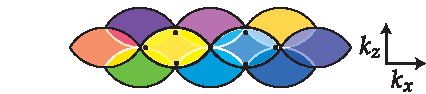
\includegraphics[width=\linewidth]{./sim/axial_3_beam}
        \caption{3-beam SIM at \SI{2}{\times}\(k_0\)\\
        3D reconstruction}\label{fig:sim_axial_3_beam}
    \end{subfigure}\hfill
    \caption[Axial view of 2 and 3 beam illumination in \gls{SIM}]{
    Axial view of 2 and 3 beam illumination in \gls{SIM}.
    Black points in (\subref{fig:sim_axial_otf}) represent lateral frequency mixing from 2-beam illumination, the grey points represent axial frequency mixing from 3-beam illumination.
    (\subref{fig:sim_axial_otf}) shows the lateral extent of 2-beam \gls{SIM} at maximum (\SI{2}{\times}) excitation frequency, with no added axial resolution.
    (\subref{fig:sim_axial_2_beam_3d}) shows the lateral extent of 2-beam \gls{SIM} at (\SI{1.5}{\times}\(k_0\)), giving reduced resolution but providing increased axial resolution.
     (\subref{fig:sim_axial_2_beam_3d}) shows the lateral and axial extent of 3-beam \gls{SIM}, doubling in resolution axially and laterally~\cite{gustafssonSurpassingLateralResolution2000}.
     The thick black outlines show the original OTF support of the widefield image.
    % Resulting OTF in (a, c) two- and (b, d) three-beam illumination. The black spots in
    % the microscope’s widefield OTFs (a: two-beam and b: three-beam) show the origins of the
    % shifted object information copies.When these copies are shifted back (c, d) to their correct
    % positions, the effective OTF increases in size. The black outline shows the original widefield
    % OTF cut-off border. The borders of the shifted OTFs are shown in gray. The corresponding
    % illumination patterns are shown in Figure 9.2a,b
    }\label{fig:sim_axial}
\end{figure}

\subsubsection{\gls{mSIM}}\label{sec:msim}

Schroff~\emph{et.~al.} showed that three dimensional, super-resolved, information can be also be extracted by \gls{mSIM}~\cite{yorkResolutionDoublingLive2012}.
\gls{mSIM} uses a square lattice of illumination points which raster scan across the sample to provide a fast, parallelised, confocal-like image.
Each spot is computationally pin-holed, and the resulting images are summed to produce a final, super-resolved image, as in \figurename~\ref{fig:mSIM}.

\begin{figure}
  \centering
  \begin{subfigure}[t]{0.185\textwidth}
    \centering
    \includegraphics[width=\linewidth]{msim/raw_excited}
    \caption{A lattice of illumination points}\label{fig:msim/raw_excited}
  \end{subfigure}\hfill
  \begin{subfigure}[t]{0.185\textwidth}
    \centering
    \includegraphics[width=\linewidth]{msim/recorded_excited}
    \caption{The image as recorded by the detector}\label{fig:msim/recorded_excited}
  \end{subfigure}\hfill
  \begin{subfigure}[t]{0.185\textwidth}
    \centering
    \includegraphics[width=\textwidth]{msim/digital_pinholing}
    \caption{Digital pin-holing}\label{fig:msim/digital_pinholing}
  \end{subfigure}\hfill
  \begin{subfigure}[t]{0.185\textwidth}
    \centering
    \includegraphics[width=\linewidth]{msim/column}
    \caption{Reconstructing}\label{fig:msim/column}
  \end{subfigure}\hfill
  \begin{subfigure}[t]{0.185\textwidth}
    \centering
    \includegraphics[width=\linewidth]{msim/reconstructed}
    \caption{Full mSIM reconstruction}\label{fig:msim/reconstructed}
  \end{subfigure} % \includegraphics{/path/to/figure}
  \caption[Schematic of \gls{mSIM} reconstruction]{
  Schematic of \gls{mSIM} reconstruction. \gls{mSIM} uses a square lattice of illumination spots in (a) and (b); which are digitally pin-holed in (c); and raster scanned in (d); to build a super-resolved image in (e)}\label{fig:mSIM}
\end{figure}

% After separation, the information can be shifted back to
% its respective position, resulting in an expanded accessible frequency area (c). To expand
% the resolution in the object plane not only along one direction but also isotropically,
% the illumination pattern is subsequently rotated to carry out the image acquisition with
% several illumination pattern orientations (d).}

% \subsubsection{Drawbacks}

\subsection{Selective plane illumination microscopy}

The techniques as introduced above all provide volumetric imaging through reconstruction.
Structured illumination techniques require computation reconstruction which is prone to artefacts.
Confocal scanning is slow and generally lossy with signal.
Light-sheet microscopy offers reconstruction-free, fast, low photo-toxicity volumetric imaging.
The application of light-sheet microscopy is the focus of this thesis and will be introduced in detail in the following chapter.

% In light sheet microscopy, the sample is illuminated with a thin sheet of light to obtain optical sections.
% The microscope generally consists of two orthogonal optical axes: one for generating the light sheet for illumination, and the other for widefield detection of the emitted fluorescence.
% The two axes are aligned such that the illuminating light sheet is positioned in the focal plane of the detection unit.
% As the specimen is illuminated with a sheet of light, the entire focal plane of the detection arm is illuminated providing instant optical sectioning as opposed to the slow point scanning used in confocal microscopy (Chapter 5).
 %1    %DONE
%!TEX root = ../../thesis.tex
%!TEX enableSynctex = true
%*******************************************************************************
%****************************** Third Chapter **********************************
%*******************************************************************************
% **************************** Define Graphics Path **************************
\ifpdf
    \graphicspath{{Chapters/literature/Figs/Raster/}{Chapters/literature/Figs/PDF/}{Chapters/literature/Figs/}}
\else
    \graphicspath{{Chapters/literature/Figs/Vector/}{Chapters/Figs/}}
\fi

\chapter{Contemporary light-sheet technology}%:\\ \Large Correlating real-time viscoelastic changes with embryonic development}

Light sheet fluorescence microscopy (LSFM) is revolutionising the way in which complex, living biological samples can be imaged at high spatial and temporal resolution. %-
The technique deviates from conventional epi-fluorescence microscopy in that one illuminates the sample orthogonally to its detection.
The decoupling of illumination and excitation allows for the construction of light sheets whereby a single plane of interest is excited.  %CITE 14,15,16.
As such the technique offers optical sectioning capability comparable to a confocal microscope whilst still using a wide field detection system~\cite{siedentpf_uber_1903,voie_orthogonal-plane_1993,huisken_optical_2004-1}. %-
This garners two key advantages: firstly, as the plane of interest being detected is irradiated, the incident photon dosage is drastically reduced and so photo-toxicity to the sample is minimised.%-
This is in stark contrast to confocal imaging where signal is collected from a small voxel along the illumination axis whilst the entire sample is illuminated when recording a single image plane.
Secondly, wide field detection enables a significant temporal resolution increase in LSFM versus confocal.
For rapid volumetric imaging of complex organisms LSFM is becoming the technique of choice in developmental biology~\cite{keller_fast_2010,verveer_high-resolution_2007,mickoleit_high-resolution_2014,icha_using_2016,keller_visualizing_2015,ichikawa_live_2014}, plant science~\cite{wangenheim_rules_2016} and cell biology~\cite{capoulade_quantitative_2011,cella_zanacchi_live-cell_2011}.

The concept of orthogonal detection and illuminations dates back to 1903 when Zsigmondy and Siedentopf studied colloids in their \textit{Ultra-microscope}.
%who used a slit aperture and Sun light to image colloids in their \textit{Ultra-microscope} over in 1903 \cite{siedentpf_uber_1903}.
Technological advances in fluorescent dyes, labelling and digital image detection has permitted Voie~\emph{et~al}~\cite{voie_orthogonal-plane_1993}
to present the first light sheet fluorescence microscope in 1993.
%advances meant that in 1993, when Voie et al
%were able to present the first light sheet fluorescence microscope.
By 2004 Huisken~\emph{et al}~\cite{huisken_optical_2004-1}
demonstrated the potential of LSFM for \emph{in-vivo} imaging with cellular resolution.
Their Selective Plane Illumination Microscope (SPIM), seeded a rapid development in the LSFM field and is chosen here as an example to discuss the main concepts of LSFM.\@
\footnote{Design choices made here have heavily influenced the openSPIM project, an information toolkit found on the internet for constructing a LSFM}

%High quality LSFM is dependent on how well the illumination is generated.
%Huisken et al seminally used Gaussian laser emissions for the generation of their light sheets. Gaussian beams have a distinct trade-off when used in LSFM applications in that the thinner the light sheet designed the narrower the field of view; this can be seen in equation \eqref{eq:Guassian}, as $x$ increases or decreases (a movement away from the focus of the beam) the wider the beam gets.

%The Rayleigh length (or confocal parameter) in equation \eqref{eq:Rayleigh} is a metric for the distance over which a Gaussian beam still propagates as if it were parallel (neither converging nor diverging), for LSFM this is the distance over which it can be assumed the light sheet is of homogeneous thickness.

%Equation
%From equation \eqref{eq:Lorrentzian} g can be seen as having a dependence on the spot size or


\section{Generating Light Sheets}

\begin{itemize}
	\item[\checked] Optically  %\tick
	\item[\checked] Virtually
	\item[\checked] Volumetric Imaging
\end{itemize}	%Lightfield is instant 3D

\subsection{Light sheet generation}
\subsection{Optical Light sheet Generation}

%High quality LSFM is dependent on how well the illumination is generated.
Huisken~\emph{et~al} seminally used Gaussian laser emissions for the generation of their light sheets despite Gaussian beams have a distinct trade-off when used in LSFM applications, in that the thinner the light sheet the narrower the usable field of view.
Equation~\eqref{eq:Guassian} models the Gaussian beam approximation where the full-width half-maximum ($\sqrt{\ln(2)}\omega(z)$) %\mynote[inline]{check maths}
increases as a Lorentzian when a distance $z$ away from the focal plane (Equation~\eqref{eq:Lorrentzian}).
The rate at which this occurs is dependent on the Rayleigh length in Equation~\eqref{eq:Rayleigh} which quantifies the trade-off.
The confocal parameter ($b=2z_R$) is a metric for the distance over which a Gaussian beam propagates as if it were parallel (neither converging nor diverging).
For LSFM this is the distance over which the light sheet can be assumed to be of homogeneous thickness.

Huisken also pioneered the use of a cylindrical lens to focus the Gaussian beam one dimensionally into a Gaussian light sheet.
The Gaussian nature of a beam's intensity for LSFM requires that the excitation beam is over expanded and later cropped by an aperture to create homogeneous illumination.
The procedure is optically lossy, but, laser intensity is typically in surplus for fluorescence microscopy techniques; a typical fluorescent sample needs $2\pm 1.5$ mW versus a low end diode laser emitting $100$ mW+.

%Huisken's SPIM had two distinct parts. The illumination path, which included a laser source beam expander to control the field of view of the light sheet and a  cylindrical lens to focus the beam into a thin sheet of light (Fig %FIGURE
%); and the detection path, which was similar to a standard widefield microscope including an objective lens, a tube lens and a camera.

\begin{align}
	I(r,z)    & = {I_0} {\left(\frac{\omega_0}{\omega{(z)}}\right)}^2 {e^{\frac{-2r^2}{\omega{(z)}^2}}\label{eq:Guassian}} \\
	\omega(z) & = \omega_0 \sqrt{1+\frac{z}{z_R}} \label{eq:Lorrentzian}                                                   \\
	z_R       & = \frac{\pi\omega_0^2}{\lambda} \label{eq:Rayleigh}
\end{align}

Where:\\
$z_R$ is the Rayleigh Length\\
$\omega_0$ is the spot of size of the beam.\\
$\lambda$ is the wavelength of light.\\

% Introduce Gaussian beam
% In cylindrical lens case laser light needs to be over expanded and cut to ensure a FOV homo

\subsection{Digital Light sheet Generation}

%Cylindrical lenses are bad because the sheet is highly coherent causing interference and more shadowing.
%A light-sheet crafted just using a cylindrical lens comes with it's own issues.
%Keller et al addressed
Keller~\emph{et~al}~\cite{keller_quantitative_2008} proposed sweeping a narrow laser beam through the sample to create a virtual light sheet.
This was achieved by oscillating galvanic mirrors at kHz frequencies, well over the Nyquist limit in comparison to the imaging acquisition rate~\cite{keller_quantitative_2008}.
To ensure a homogeneous illumination and distributed photon dosage a tele-centric f$\theta$ lens was used to convert beam angle optically from the scanning mirrors in to a linear position~\footnote{A practice borrowed from laser scanning microscopy.}.

Using DSLM instead of a cylindrical lens based system offers some key advantages.
Firstly, as the beam is scanned rather than stretched there can be no optical interference of coherent photons between neighboring regions, this reduces speckles and shadows.
Secondly, illumination intensity can be modulated such that structure can be superimposed on the sample giving the potential for super-resolution image improvement.
This resolution improvement has so far solely been experimentally demonstrated in the direction of the the scanning due to geometrical constraints~\cite{chen_lattice_2014}.

\subsection{Volumetric imaging}

The true power of light sheet microscopy becomes evident in its fast volumetric imaging capability.
Huisken's original SPIM required samples to be mechanically scanned through the static light sheet, potentially disturbing the sample depending on the speed of the scanning.
dSLM has the potential to subvert the static light sheet by using a second galvanometric mirror to move the light sheet relative to the static sample, the detection objective is then mounted on a high speed and precision axial translator and tuned to follow the light sheet.
Ideally piezoelectric actuators are used as their settling times are on the order of milliseconds providing speed and accuracy needed to match 100Hz cameras.
Of course, with dSLM, instead of the sample motion causing a disturbance a large objective local to the specimen is causing turbulence.
This was matched optically through the use of an electrically tunable lens~\cite{fahrbach_rapid_2013-1} that moves working distance of the detection objective.
%As such a new method was developed to achieve this optically, by using an electrically tunable lens to adjust the working distance of the detection objective.
This technique suffers from: fluorescent signal losses in the further four lenses and two mirror surfaces
\footnote{The mirrors are used to ensure the ETL is horizontal to gravity as further aberrations occur if the tunable surface is not entirely flat.
In essence two mirrors from the tunable light sheet could be removed by using mechanically deforming tunable lenses instead of electro wetting tunable lenses.}
($\sim 80$ percent signal retrieved); spherical aberration and is a more involved method as the system requires a non-linear calibration.


%Image of four configurations with details.
\section{Objective Arrangements}
\subsection{Single View}
%To ensure compatibility of Light sheet microscopes with biological mounting arranging.
Light-sheet microscopes are distinct in that two objectives are used orthogonally causing the technique to incompatible with most standard epi-fluorescent biological mounting practices.
Efforts have been made to make light sheet imaging more accepted through novel objective arrangements as well as new and intuitive mounting approaches.

\subsubsection{Horizontal Orientation}

\begin{itemize}
	\item[\checked]  Flat (openSPIM) open-SPIN diy-SPIM
				\item[\checked] MuVIEW\cite{swoger_multi-view_2007}%CITE"3060
	\item[\checked] Vert
	\item[\checked] V (diSPIM)
	\item[\checked] 60/30		Lattice Light Sheet and Objective Compatibility (Short section)
	\item[] Multi VIEW
\end{itemize}

%and the excitation objective illuminating through a clear window in the chamber.
Huisken~\emph{et~al.}, for instance, used two objectives in a horizontal configuration with a detection objective built into the sample chamber whilst the illuminating through a clear window.
This configuration was chosen so that a sample could be lowered into the system and, crucially, rotated without gravity causing registration errors when reconstructing the volume tomographically.
Rotational volumetric imaging also minimises shadows and improves image quality lost to scattering especially in thick (>$500 \mu m$) samples.
Mounting a sample from below and rotating produces the same result but requires a more sophisticated chamber design to contain the sample medium.
A horizontal geometry is vital also for plant biology as the objectives do not inhibit the plant's natural tendency to be upright~\cite{wangenheim_rules_2016}. %TODO CITE Stelzer
%Long working distance detection objectives have also been considered but the the lowered NA and

\subsubsection{Vertical Orientation}

An alternative to the Huisken's horizontal configuration is positioning the detection objective above the sample and illuminating from the side.
A vertical orientation is an attractive option as it can be compatible with commercial optical microscopes as well the chamber not requiring an inbuilt detection objective. %CITE 29 30
Both of these techniques can allow at  additional illumination objective, by offsetting the foci of the illumination objectives an overall more homogenous field of view can be created.


\subsubsection{(45 $^o$ Orientation)}

Shroff~\emph{et~al} then pioneered use of two objectives in a V configuration above the sample through iSPIM.\@
With choice objectives, adhered samples prepared with standard mounting procedures can be imaged in a petri-dish~\cite{kumar_dual-view_2014}.
%Other group then did the 45 degree inverted iSPIM.
%Shroff's diSPIM~\cite{kumar_dual-view_2014} then drastically improved axial resolution by imaging through both arms of the microscope.
%In doing so the axial resolution not collected through one arm is directly observed in the other.

%CITE 30 chick embryos

\begin{figure}
	\centering
	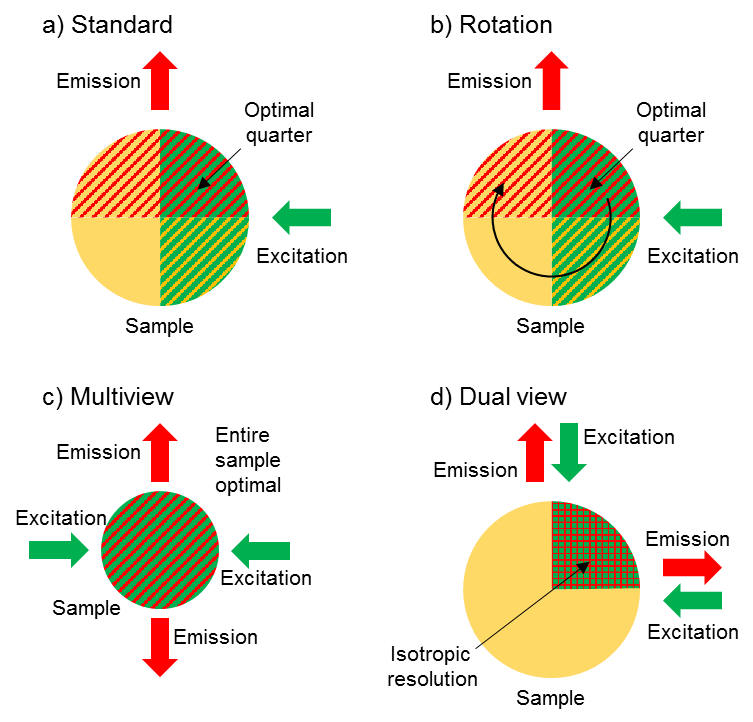
\includegraphics[width=\columnwidth]{spim_optimal_imaging.png}
	\caption{
	(a): The simple SPIM field of view – only a quarter of a sample has optimum illumination (green) and excitation (red).
	(b): by rotating a sample field of view can be quadrupled but at a cost in acquisition time. (c): By adding extra excitation and detection path the entire sample can be imaged without a rotation.
	(d): by making optical paths of a LSFM dual purpose a quadrant of a sample can be imaged from two orthogonal perspective and with correct image fusion achieve isotropic resolution.
	tod}
	\label{spim_optimal_imaging}
\end{figure}

\subsubsection{Optimal Orientation}

In a bid to maximise sample accessibility and numerical aperture, Betzig~\emph{et~al.}~\cite{chen_lattice_2014} commissioned a high NA (0.6) custom excitation objective to fit with their high NA (1.1) detection objective (Nikon CFI75).
In mounting the orthogonal pair at an angle such that they were flush so a flat surface, Betzig~\emph{et~al.} created the most unhindered sample mounting conditions realistically feasible using two objectives.
Tricks to circumvent objectives interfering with sample mounting are needed as high NA objectives are physically large.
%Numerical aperture depends on the $\sin$ of the collecting angle of light , intuitively this requires that the detecting objective to awkward in non-epifluorescence orientations. \mynote{reword}
%Moreover, the desire for high resolution images can cause spacial incompatibility between both objectives.
Moreover,  high NA objectives typically have short working distances and require both objectives to be close, and likely cause spacial incompatibilities even with the narrowest excitation objectives.
See figure~\ref{fig:objectivecompatibility} for a detailed comparison.

\begin{figure}
	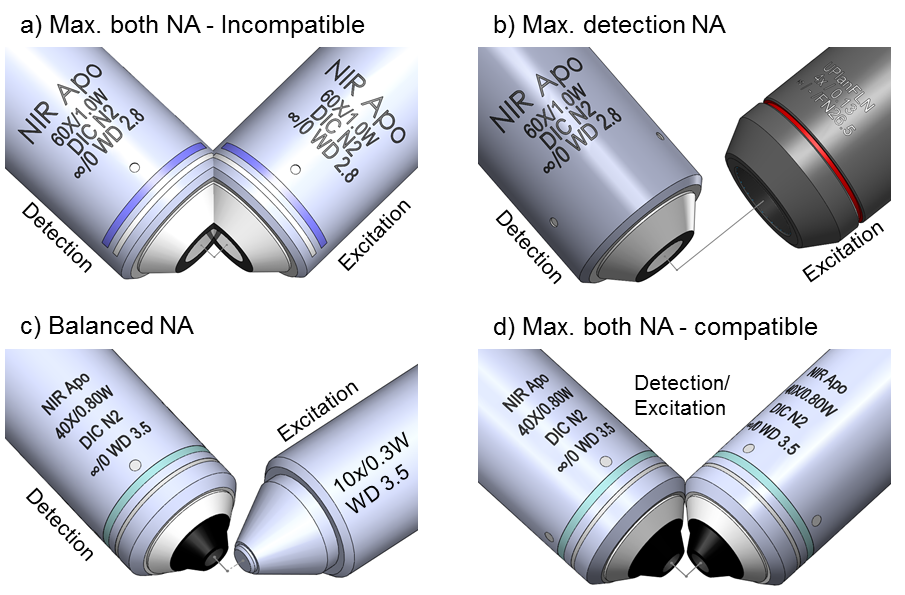
\includegraphics[width=\columnwidth]{objectivecompatibility}
	\label{fig:objectivecompatibility}
	\caption{}
\end{figure}

%Gaussian light sheet systems do not typically require such large NA excitation objectives meaning there are standard excitation objectives available.
%High NA objectives tend to have limited working distance and, in the orthogonal arrangements required for LSFM, have to be positioned very close to each other.

%suitably narrow such that flat substrates could be imaged.
%lattice light sheet style custom excitation.

%Gaussian beams don't need high NA excitation optics
%Large NA detection objectives have large collecting angles so a long working distance objective in desirable.


%subsection{MultiView}
\subsection{Multi-View}%\cite{swoger_multi-view_2007}

Shroff~\emph{et~al} introduced alternately imaging between each objective of the iSPIM in the form of the diSPIM~\cite{kumar_dual-view_2014}. %TODO Repeating myself
\footnote{This system is now a commercial light sheet solution provided by ASI.}
Axial resolution that would otherwise be lost to thick light sheets is recovered by switching the imaging and detection arms.
The two data sets captured by each camera are fused in post processing to provide near isotropic three dimensional resolution.
%\subsubsection{DualView}
%Shroff~\emph{et~al} not only pioneered the inverted SPIM (iSPIM) concept but also introduced alternately imaging between each objective in the form of diSPIM~\cite{kumar_dual-view_2014}. %TODO Repeating myself
%Axial resolution that would otherwise be lost to thick light sheets is recovered by switching the imaging and detection arms.
%The two data sets captured by each camera are fused in post processing.
%subsection{MuVU}
Where LSFM provides the most improvement over other techniques, such as in large, thick biological samples
%Where LSFM provides most improvement over other techniques
, scattering becomes significant both for excitation and emission light.
diSPIM however does not address inherent issues of scattering in thick samples, there is an \emph{optimal quarter} (see Figure~\ref{spim_optimal_imaging}) wherein excitation and emission photons are the least scattered.

Krzic~\emph{et~al} returned to the horizontal orientation of Huisken's SPIM, and chose their objectives wisely in MuVU-SPIM where two excitation and two detection objectives were packed around a hanging sample. %cite objectives (Krzic et al. 2012)
MuVu can reach all regions of its sample, but it cannot dodge scattering limitations homogeneously.
%\subsection{Tomography}
To minimise gross scattering, sample rotation is necessary, of course acquiring volumes tomographically raises its own unique issues such as volume registration, rotational synchonisation and lengthy acquisition times.
Regardless, for large samples two objectives in Huiksen's original SPIM provide a cost effective robust volumetric imaging solution; with projects like the OpenSPIM have received significant acceptance and community attention.

\section{Single Objective Light Sheet Microscopy}

\begin{itemize}
	\item[\checked] Axial Plane \cite{li_axial_2014}
	\item[\checked] Oblique Plane \cite{dunsby_optically_2008}
	\item[\checked] Fibre SPIM \cite{ploschner_multimode_2015}
	\item[\checked] Mirrored Cuvette,
	\item[\checked] Confocal adaptor
\end{itemize}

Prior to refinements in objective positioning Dunsby conceptualised a system for single objective light sheet microscopy.
The advent of such systems could provide a plug-and-play light sheet experience on commercial microscope frames.
Dunsby proposed illuminating the sample using a high NA objective whereby the light sheet would illuminate at an oblique angle to the optical axis, the detected signal is then retrieved using the same objective~\cite{dunsby_optically_2008}.
Optically the sample is conjugated to a virtual position where a pair of objectives (excitation and detection) analyse the virtual sample in a conventional light sheet manner.
The technique suffers from optical technology, only when using a high NA objective can the system fully capture detection perpendicular to excitation.
Unfortunately, OPM is an involved technique as it requires that a standard light sheet microscope is constructed behind a further optical relay system.

Virtual sample manipulation is alluring as one can perform virtual manipulations that in are physically impossible.
Zhang et al~\cite{li_axial_2014} created their virtual sample using a similar relay system to Dunksby\emph{et~al}, but crucially they positioned an atomically flat mirror which precisely rotated their virtual sample by $90^o$.
In doing so they could illuminate the real sample along the optical axis and their virtual projection from the mirror was imaged directly onto a camera using a standard wide field configuration.

Using small mirrors near the sample is another viable, though more restrictive, approach to single objective LSFM.\@
Galland~\emph{et~al.} fabricated  micro-wells with $45^o$ micro-mirrors~\cite{galland_3d_2015}, converting any commercial scanning microscope into a light sheet microscope.
Leica produce a similar solution in the form of an objective adapter which holds two mirrored surfaces near the sample creating a similar effect.
Both techniques limit the size of the sample and their sectioning capability heavily depends on the quality of the mirrors used.

Ploschneret al.~attempted to minimise the size of the second objective rather than remove it.
By substituting the second objective for a multimode fibre~\cite{ploschner_multimode_2015} not only could they provide more access to their samples, but they could also embed their excitation source into their imaging chamber.
Assuming that a multi-mode fibre operates deterministically on an input light source, they were able to correct for the fibre using an SLM and further demonstrated the system's ability to produce exotic beam profiles.

%TODO cite scape

%subsection{Axial Plane}~\cite{li_axial_2014}
%subsection{Oblique Plane}~\cite{dunsby_optically_2008}
%subsection{Fibre SPIM}~\cite{ploschner_multimode_2015}

%Optical fibre transforms input light, can comepnsate and produce light sheets, bessel light sheets and lattice etc. Demonstrated in 0.25 NA fibre. Could use soft glass fibre to prove concept further.

%subsection{Confocal adaptor}

% High NA objectives require short working distances and large apetures
% An asymmetric pair
% an NA of 0.3 is needed to create a micron thick miaskla kzas
% Gaussian beam illumination requires low NA excitation and so assymetric pairs are ideal with a high NA detection being then possible (with a loss of axial resolution)
% Bessel illumination however requires high NA to construct the thin buy extended sheets and so are commcercially infeasible. Betzig et al. notabley used a custom excitation objective.
% Biological samples should be given room.

% Hence the ‘vertical at 90o’ approach can very attractive even if it cannot boast high NA excitation.  Another limitation arises from geometrical compatibility of the objectives i.e. their opening angles cannot exceed 90o and the front lens radius of one objective should not exceed the working distance of the other objective.

%High NA detection and low NA excitation leads to high lateral resolution and low axial resolution.

\section{Illumination}

%\begin{itemize}
%	\item Variable Gaussian $\box$
%	\item Bessel\cite{gao_3d_2014}
%	\item Lattice light sheet.\cite{chen_lattice_2014}
%	\item Airy Beam $\box$
%	\item Multi-photon \checkmark~\cite{truong_deep_2011}
				%Comparison of Cost and Complexity?
%\end{itemize}

\subsection{Gaussian Techniques}
Illumination techniques have been proposed in a bid to circumvent the ubiquitous Gaussian beam extension versus thickness trade-off.
The most intuitive approach is accepting the loss of FOV produced by Gaussian illumination and moving the focus of this strip of high axial resolution light to different parts of the sample.
A final image can then be fused to achieve maximum axial resolution though with a direct cost for time of acquisition and photobleaching versus axial resolution, with an exceptionally high NA light sheet tending to becoming as slow and damaging as a confocal system . \mynote{CITE Variable light-sheet.}
Fu~\emph{et~al.} proposed tiling multiple thin Gaussian light-sheets that are focally offset to create a similar tiling effect without the temporal loss~\cite{fu_imaging_2016}.
%The technique of tiled light-sheets was proposed recently whereby multiple thin Gaussian light-sheets are superimposed and focally offset to create a similar tiling effect without the temporal loss \cite{fu_imaging_2016}.
This effect was produced by using a Spatial Light Modulator whose hologram had superposed lens-like phase patterns superimposed.
This technique again suffers from the additional photo-dosage imparted by the undesirable lobes of the Gaussian beam, moreover these low resolution sections also contribute to fluorescent background reducing the net SNR of the system.
\subsection{Exotic Beams}
Species of exotic beam do exist which do not subscribe to classical Gaussian beam limitations.
%Airy beams, for instance, are non-diffracting, self healing beams.
% and I don't know anything about them over that Nikon use them?
Bessel beams are non-diffracting and self healing, meaning they reconstruct behind occlusions making them very desirable for light-sheet applications.
They can be optically constructed from either an axicon lens or a amplitude mask with a annual ring opening, the latter being inexpensive but the most optically lossy.
Unlike Gaussian optics their extension and thickness can be theoretically entirely decoupled, in practice a Bessel-Gauss beam only behaves over short distances \cite{gao_3d_2014} of up to $\sim 30\mu m$.
%\mynote[inline]{how short?}
% with the thickness being controlled by the outter-most radius and their extension
%Be beams both self heal,
Bessel beams however suffer from having multiple undesirable orders, the more ideal a Bessel beam is the more intensity is retained in its outer rings.
As such a singular scanned Bessel beam itself causes a significant background.
Betzig~\emph{et~al.}\cite{chen_lattice_2014} exploited these additional orders, they constructed multiple Bessel beams in the scanning plane by superimposing a sinusoidal amplitude pattern on to an annular amplitude mask.
In doing so their undesirable orders constructed to reinforce the zeroth orders of the parallel beams.
Finally they adjusted their now lattice light-sheet such that the outer orders above and below the scanning plane lay at minima in the detection point spread function reducing the net fluorescent axial background.
\subsubsection{Airy Beams}
Airy beams also self-heal similarly to Bessel beams but comparatively are more extended.
They are constructed using a coma-like phase pattern and exhibit characteristic a beam curvature.
Though they extend several fold further than Bessel beams, their curvature produces an asymmetric profile along the detection axis.
This is then required to be deconvolved in post processing.
Vettenburg~\emph{et~al}\cite{vettenburg_light-sheet_2014} demonstrated similar axial resolution improvement to Bessel beams whilst achieving a $\sim 3$ increase in field of view.
%It logically follows to create a lattice of Airy beams, this
%\mynote[inline]{TODO cite.}
%Airy beams are generated with a phase distribution resembling coma aberrations. These beams are characterised by longer extent compared to typically achievable Bessel beams (e.g. extension of 160 µm versus 60 µm for a Bessel beam with similar diameter) (Vettenburg et al. 2014). However, the Airy beams exhibit a curvature similar to coma aberrations and unsymmetrical higher orders in the beam radial profile, creating a PSF with characteristic unsymmetrical elongation along the detection axis (Morris et al. 2009). These can be corrected by deconvolving a measured stack using software methods. This can produce better resolution images with larger field of view compared to similarly deconvolved images obtained using Gaussian and Bessel beams (Vettenburg et al. 2014). However, this superiority over Bessel beams has only been demonstrated in comparison with the most basic Bessel beam setup, which does not compensate for higher orders of the Bessel beam distribution

\begin{figure*}
	\centering
	\label{fig:scatteringandshadowing}
	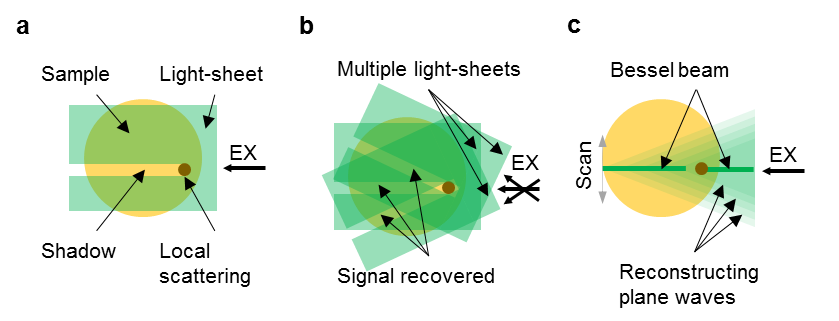
\includegraphics[width=\textwidth]{scatteringinlsfm}
\end{figure*}
\subsection{Thinner Beams}

Attempts to quantum mechanically narrow Gaussian Light sheets include using stimulated emission depletion and two photon emission (2P).
Using an addition laser to deplete, through stimulated emission (STED), out of plane fluorescence can narrow a Gaussian light sheet to $<1 \mu m$ \cite{friedrich_sted-spim:_2011}.
Two photon light sheet microscopy requires an excitation from two concomitant photons of cumulative energy sufficient bridge the required energy gap.
This requirement ensures that such excitation events are sufficiently rare and only occur where photon density is high.
%This requirement drastically reduces
%narrows the region in which fluorophores are likely to excite.
%By that two photons of cumulative energy sufficient to bridge the required energy gap, .
%By requiring that a fluorescent excitation only occurs when two photons of wavelength double that of the required energy gap,
In epi-fluorescent microscopes this occurs in the focal plane with the probability reducing quadratically along the imaging axis.
In light sheet microscopes this occurs at the axial centre of the light sheet making it much thinner than a comparable 1P excitation sheet.

%Exciting a
 %2    %DONE
%!TEX root = ../../thesis.tex
%!TEX enableSynctex = true
%*******************************************************************************
%*********************************** First Chapter *****************************
%*******************************************************************************

\definecolor{455nm}{RGB}{0,97,255}
\definecolor{488nm}{RGB}{0,247,255}
\definecolor{561nm}{RGB}{198,255,0}
\definecolor{647nm}{RGB}{255,0,0}
\definecolor{illustrator_red}{RGB}{226,7,25}
\definecolor{illustrator_green}{RGB}{0,150,64}

\ifpdf
    \graphicspath{{Chapters/design/Figs/Raster/}{Chapters/design/Figs/PDF/}{Chapters/design/Figs/}}
\else
    \graphicspath{{Chapters/design/Figs/Vector/}{Chapters/design/Figs/}}
\fi

% Chapter 3.	Microscope design
% 3.1	Design objectives	59
% 3.2	Optical design	59
% 3.3	Mechanical design	64
% 3.4	Assembly	67
% 3.5	Control	68
% 3.6	Orientation, Alignment and Calibration	73
% 3.7	Initial results	74
% 3.8	Design summary	81


\chapter{Light-sheet microscope design and considerations }\label{chapter:design}

% \epigraph{\emph{It doesn't have to be good, it just has to look good.}}%{--- Anonymous}
%Physical prciniples of the operation of a light-microscope.
%Capabilities limtiations.

This chapter introduces the instrument which was built and used during this thesis.
It was required that the system presented here facilitated a wide range of imaging challenges, with two specific %biological aims to be met.
imaging tasks to be performed.
The first %of which task required the system to
task was to image \gls{zebrafish} embryos (\SI{\sim500}{\micro\meter}), surrounded by a magnetic tweezer system, during the \SI{1}{}k~cell stage of embryo development (see Chapter~\ref{chapter:tweezers}); this was for the study of developmental mechanobiology.
The second required the imaging of live (\gls{SH-SY5Y}) mammalian cells (\SI{\sim50}{\micro\meter}) for viral particulate tracking; this was for the study of 3D-live-cell viral egress using \gls{SPT}.

The instrument developed here was a complete rebuild of a previous instrument, certain individually components were transferred through but the entire hardware and software scheme was redesigned and assembled~\footnote{Rebuilt twice as the microscope moved buildings half way through this thesis.}.
\pagebreak
\subsection*{Specification}\label{sec:specification}

To facilitate these biological aims the system has to address these specification key criteria:

\begin{enumerate}
    \item Fast volumetric imaging, 1 volume per second for the pixel range:\\\SI{2048x2048x100}{}\label{item:volumes}
    \item Multi-colour interlaced volumetric imaging\label{item:colour}
    \item Capacity for multiple methods of sample mounting\label{item:mounting}
    \item Multiple imaging length scales, \gls{FOV} range:~\SIrange{200}{700}{\micro\meter}\label{item:scales}% magnifications
    \item Options for exotic illumination development through optional illumination paths to incorporate an \gls{SLM}\label{item:illumination}
    \item User-friendly and extensible software scheme in \gls{LabVIEW}\label{item:software}
\end{enumerate}

% \subsection{Embryonic imaging for Mechanobiology}
%
% For embryonic imaging using magnetic tweezers the system had to be designed with sufficient space
%
% \subsection{Cellular imaging for Viral Egress}
%
% To realise particle tracking within light sheet microscope improvements upon the previous system were considered and the entire microscope was to be rebuilt using a new design.
% Any optical development project comprises of a series of sub-systems, modules which can be built and designed so that the overall scale of the project is made more manageable.
% A microscope of this nature will have typically four aspects:
%
% \begin{itemize}
% 	\item Sample Holding
% 	\item Illumination
% 	\item Detection
% 	\item Image Acquisition
% \end{itemize}
%
% Though each section may somewhat affect the others key decisions and debugging can usually be localised to each.
% This section will discuss the new design, improvements upon the previous design and the current build state of the microscope for each of these components of the new system.

\section{Hardware}

The design presented here is an adaptation of a previous \gls{light-sheet} microscope~\cite{chmielewskiFastImagingLive2015}, whose entire optical assembly was mounted on a set of rails rotated at \SI{45}{\degree}.
The upgrade and redesign of the system was made such that the illumination and detection paths of the new system could be extended so that liquid tuneable lenses could be mounted in the vertically to reduce gravity induced optical aberrations.
% The new design presented in this thesis adapts a previous design.
For precise tracking of single virions, a more stabilised method of suspending the microscope objectives was needed as this minimises vibrational blur.
This was problematic in the previous design due to design using cantilevered detection optics away from the frame, causing general instability.
% suspension of objectives was needed.

\subsection{Mechanical design}

% \gls{illumination arm}
% \gls{detection arm}
% \gls{imaging board}
% \gls{illumination board}
% \gls{imaging optical rail}
% \gls{illumination board}
% \gls{imaging board}

The mechanical design of the \gls{light-sheet} microscope consists of two optical breadboards, mounted one above the other.
One for mounting the light sources (\gls{illumination board}) and the second (\gls{imaging board}) for the \glslink{illumination arm}{illumination} and \glslink{detection arm}{detection} arms.
The \gls{imaging board} was mounted vertically above the \gls{illumination board} on \SI{50.8}{\milli\metre} stabilising metal posts, which ensured the system was transportable as well as robust against vibrations.
A large rectangular section of material was removed from the \gls{imaging board} to allow the objective lenses to reach down to the samples inserted from below; too large of a gap would lead to excessive sag and vibrations in each arm, too small would impede access to the sample below the imaging board.
The objective lenses and detection objective actuator were mounted on rails at \SI{45}{\degree} to the \gls{imaging board}, the \glslink{illumination arm}{illumination} and \glslink{detection arm}{detection} arms.
These rails guided the objectives through the open section until the focal points of each objective (detection and illumination) met.
The filter wheel was placed on the \gls{imaging optical rail} before the camera and after a turning mirror on the \gls{detection arm}
% and auxiliary supports
so that the vibrations, due to
 % so that vibrations of
filter switching and the camera fan, would be mostly decoupled from the detection optics.
The camera was mounted at \SI{45}{\degree} on a \gls{3D} printed mount that corrected for the turning mirror on the \gls{imaging optical rail}.
Rotating the camera was necessary as it allowed the camera shutter and illumination beam to propagate concomitantly for slit-scanning, see later Chapter~\ref{chapter:dualslit}.

For the illumination path, a \SI{22.5}{\degree} mirror
(to the horizon, see \figurename~\ref{fig:soldiworks_top})
was used to deliver the laser illumination from the scanning optics into the illumination objective on the \gls{illumination arm}.
The additional mirror was needed so that the scanning optics could be mounted flat to the optical breadboard, making positioning and optical mounting simpler.
Using two mirrors also provided the sufficient degrees of freedom to align the axis of the scanning optics to the optical axis along the \gls{illumination arm}.
Finally, the light-sheet generating mirror of the scanning pair of was suspended off of the edge of the breadboard for delivery of the  illumination from the bottom optical table, see \figurename\ref{fig:soldiworks_top}.

% Mechanical design changes for more stable an extensible system than previous work.
% Large detection area for future upgrades on detection arm - Like my relaying
% Space below for exotic excitation and large complex biological chambers, see Tweezers Chjapter.

%The small reflection angles required by the SLM and long detection FLIM arm were incompatible with the LSFM system and a new mechanical design was necessary (Figure 7.2).


%Instead of positioning all the optical components in the 45o frame, only the detection path, the excitation objective and the tube lens were mounted at this angle.
%A mirror at 22.5o to horizontal reoriented excitation path vertically.
%Hence, a simpler frame was sufficient, consisting of two optical breadboards – one above the other.
%The dSLM optics and detection was mounted on the top level, while SLM and laser on the bottom level.
%A hole was cut in top breadboard so that the ‘V’ shaped arrangement of objectives was suspended below it.
%The sample translation stage was placed on the bottom breadboard and elevated to reach the imaging volume.
%The detection cage system included a 450 mirror which ensured that the long FLIM arm could be mounted horizontally above the top breadboard.

% Besides additional compatibility with upgrades, this design was more mechanically stable and had a large sample space for complex biological chambers.
% Moreover the tuneable lenses were positioned horizontally in a vertical cage system avoiding gravitational deformations and hence aberrations.

\subsubsection{Sample mounting}

%SPIM is notorious for sample mounting within the microscopy community, this is due to
Sample mounting using light-sheet microscopes can be challenging due to the need to place a secondary objective (for illumination) within close proximity to the detection objective.
The concept of the \gls{iSPIM}~\cite{wuInvertedSelectivePlane2011a} allows more freedom in terms of sample mounting as more of the image volume is accessible.
The \gls{imaging board} was mounted \SI{500}{\milli\meter} above the \gls{illumination board} so that an XYZ translator, with a large axial range, could be mounted.
This allowed for multiple potential sample mounting strategies below.
%This design point is one of the axioms of the new system, the focus of this report.

%The microscope system was designed using \SI{45}{\degree} \textbf{C}omputer \textbf{A}ided \textbf{D}esign so that two objectives would be mounted on \SI{45}{\degree} rails, allowing a detection and excitation objective to be lowered into a imaging space below.
%Each rail comprised of two \SI{16}{\milli\meter} to \SI{8}{\milli\meter} caging conversion mounts.
%The \SI{16}{\milli\meter} mounts were attached to the rail by two guides placed in parallel to ensure that the objectives were in the same plane and correct angle.
%The objectives were held on \SI{8}{\milli\meter} caging which attached to a thumb-screw mount holding each objective, so that they could both be very precisely lowered for fine adjustments.
%The \SI{8}{\milli\meter} caging also carried an aluminium cube suitable for dynamically lowering a beam splitter or mirror into the system so that issues on excitation could be diagnosed, as the diverted light would be the exact the image of the back aperture of the excitation objective.
%Each rail was then mounted on an optical breadboard, with a noise dampening core to limit vibrations.

%To allow the inverted objectives access to the samples the optical breadboard was cut with sufficient tolerance to allow them through but maintaining their stability; too large of a gap would cause sag in each arm, too small would impede access to the sample below.
%The hole was calculated using precision Solidworks, see Figure \ref{fig:solidworks_design_front}.
%This breadboard was then elevated to a height of \SI{50}{\centi\meter}, using $25mm$ diameter aluminium posts for stability and vibrational dampening.
%The posts were mounted on a secondary optical breadboard which supported excitation optical components.
%The secondary breadboard was implemented with the ambition that the entire microscope could be ``portable" as it did not have a permanent residence where it was being built.
%Hardware as well as a digitally controlled XYZ stage was placed on the bottom breadboard.

\paragraph{XYZ stage}

A \emph{Prior} Pro Scan \textit{HLD117} XY stage was mounted on top of a Motorized Linear Axis \textit{FB204E} Z stage.
The set was chosen as each component had integrated linear encoders, giving a suitable positional resolution (\SI{20}{\nano\meter} in \(xyz\));
speed \SI{300}{\milli\meter\per\second} in \(xy\) and \SI{15}{\milli\meter\per\second} in \(z\);
large travel range (\(\SI{120}{\milli\meter} \times \SI{72}{\milli\meter} \) in \(xy\) and \SI{38}{\milli\meter} in \(z\)). % and versatility in terms of mounting onto the microscope and sample mountings and their ability for computer interfacing~\cite{Hu2014}.
Each component was also computer controllable, and an open-source \gls{LabVIEW} routine was developed and made freely available for this purpose~\cite{russellSpimcontroller2017}.
%
% \subsubsection{Comparison with old SPIM}
%
% The original SPIM design also used a dual inverted layout, but crucially, its detection and excitation arms were not as well seated.
% Each arm was held orthogonally to gravity, meaning each acted like a cantilever, bending unstably and unpredictably under its own weight.
% This moment meant that the system was less stable than the new design and very susceptible to vibrations, which add systematic noise that can not be corrected for.
% The old SPIM also lacked in that it did not have any motorised XYZ translation, this meant that is could not achieve large area imaging, high-throughput experiments nor could it facilitate single particle tracking in thick samples.
%\subsection{iSPIM Design}
%All demonstrations of the 4~pt correction were performed on an iSPIM (\emph{inverted Selective Plane Imaging Microscope}).
\begin{sidewaysfigure}
  % \begin{figure}
  \centering
  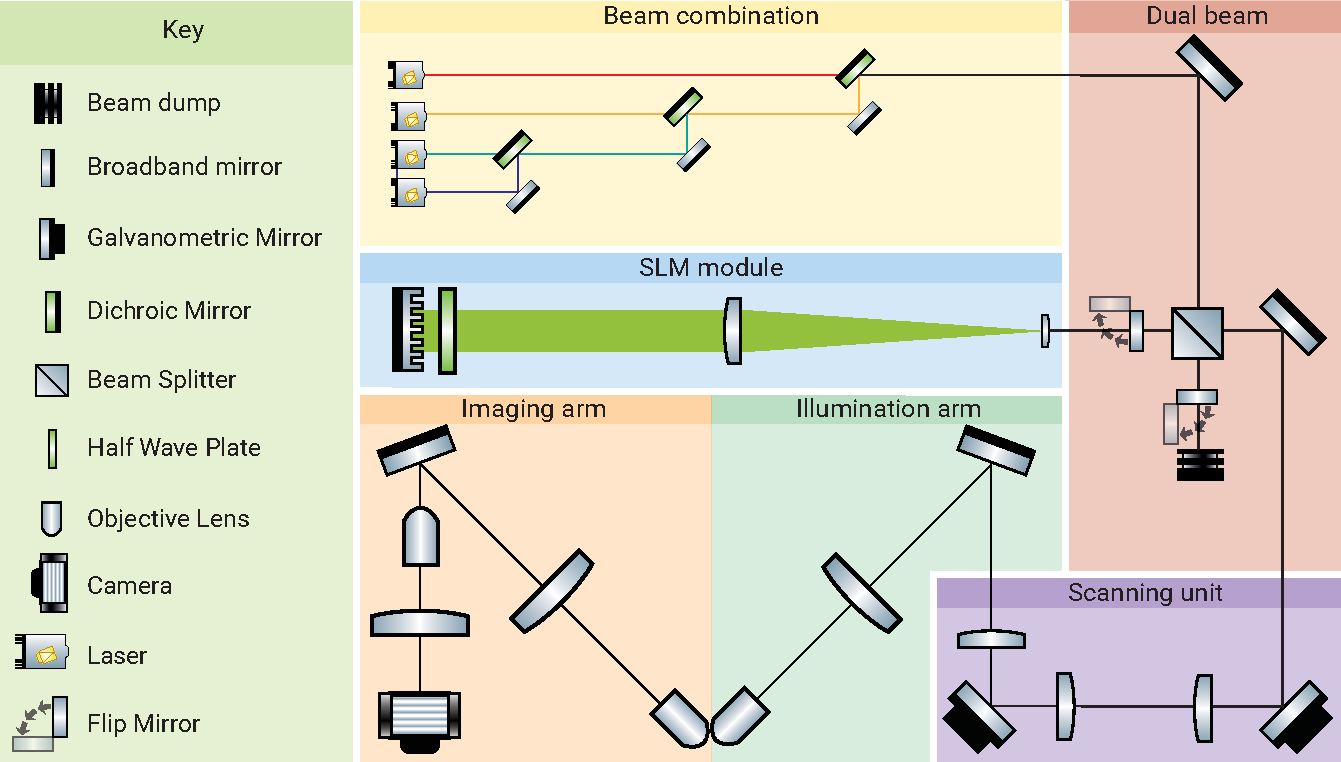
\includegraphics[width=\linewidth]{./optical_design_colour}
  \caption[Full optical design of new \gls{light-sheet} microscope]{
  Optical design of the light-sheet microscope. \textbf{Yellow:} Beam comination of the four laser lines using dichroic mirrors.
  \textbf{Red:} a beam splitter is used to create two beam arms which can be used together to create two parallel beams; one beam for single beam light-sheet; or one beam structured using the SLM (blue).
  \textbf{Blue:} Expansion optics for the optional SLM arm of the illumination system.
  \textbf{Purple:} A pair of scanning galvanometric mirrors are relayed onto each other and passed through a scan lens.
  \textbf{Green:} The illumination arm where the scanning beam is demagnified onto the sample.
  \textbf{Orange:} The high NA detection optics magnify the sample onto a second magnifying relay system and finally onto the camera.
  %Optical design of the new SPIM microscope.
  %Straight black lines represent mirrors; arrowed lines represent lenses; coloured lines represent laser light.
  }\label{fig:optical_design_colour}
  % \end{figure}
\end{sidewaysfigure}

% A (\emph{Coherent Obis 561nm}) laser was used as the beam source.
% A pair of galvanometric mirrors (\emph{Cambridge Technology}) were used to produce 2D beam steering via an image relay, this approach is well established in scanning microscopy and is known to introduce ordinarily negligible field curvature.
% A telecentric scan lens (\emph{A1 Scan Lens} from Nikon) was used to convert beam angle to beam position; %\footnote{The exact make and model will not be mentioned the manufacturers do not wish for characterisation data to be published without their express permission}
% within the observation volume this acts to keep the sweeping beam parallel for a homogenous illumination and background.
% A (\emph{10x 0.3 NA Nikon}) water dipping objective was used for excitation and mounted at right angles to a (\emph{25x 1.1 NA}) Nikon LWD water immersion objective.
% The fluorescence collected by the detection objective is then imaged onto a Hamamatsu sCMOS Orca Flash 4.
% A piezo scanner (\emph{Physik Instrumente P-726 PIFOC high-load objective scanner}) was used to manually move the detection objective to match the detection focal plane to the excitation plane.
\subsection{Optical design}

\subsection{Objective lenses}

%\nomenclature[z-WD]{WD}{WD of View}

A (\emph{\(10\times 0.3 \gls{NA}\)}) Nikon water-dipping objective was used for illumination and mounted at right angles to a (\emph{\(25\times1.1 \gls{NA}\)}) Nikon LWD water immersion objective.
The illumination objective used here has a \SI{3.5}{\milli\meter} \gls{WD} and narrow physical profile; meaning that when matched with the bulkier high NA detection objective
there would be mechanical overlap if collimated light was coupled into the illumination lenses;
instead, the illumination tube lens transmitted slightly diverging light to the back aperture of the illumination objective, which was found to efficiently resolve the challenge of separating the detection and illumination objective lenses.
%there was a slight mechanically interference, which was corrected for using the tube lens to adjust the working distance.
%, once their positioned with their foci were co-aligned.
Very few objective pairs maximise detection and illumination \gls{NA} whilst being water dipping and compatible, and a solution presented in Chapter~\ref{chapter:chamber} was found to be effective for imaging.
A piezo scanner (Physik Instrumente~\emph{P-726 PIFOC high-load objective scanner}) was used to manually move the detection objective to match the detection focal plane to the illumination plane.

\subsection{Illumination}

Four %typical
laser sources were chosen to allow good specificity across the visible spectrum as well  as for multi-colour imaging.
%, future-proofing and overall versatility in the microscope.
Wavelengths \textcolor{455nm}{\SI{455}{\nano\meter}},  \textcolor{488nm}{\SI{488}{\nano\meter}},  \textcolor{561nm}{\SI{561}{\nano\meter}} and \textcolor{647nm}{\SI{647}{\nano\meter}} were chosen to excite typical fluorescent exciters of commercially available fluorophores in the visible range.
The output power of the lasers (\SI{100}{\milli\watt}) was sufficient for good contrast images in SPIM.\@
\footnote{SPIM is within the single sun power regime} %TODO expand
%A beam quality $M^2$ nearing 1 is good, with $M^2 = 1$ being a theoretical ideal.
%Over the range of a metre the lasers will diverge by \SI{1.2}{\milli\meter}, though this would double the beam diameter the sizes are appreciably small that it will have very little effect when corrected for through later optics.
%See Table \ref{table:laser} for a detailed specification.
The beams were combined %into an overlapping beam using a set of standard dielectric mirrors and dichroic mirrors.
%Using two mirrors per beam allowed the degrees of freedom to accurately combine the beams in free space.
using dichroic mirrors % were chosen to ensure the each laser line propagated freely when approaching from behind the mirror but the correct colour laser was reflected appropriately; they were placed in the order e02 (dielectric as the first laser does not combine with any others)
(Chroma~\emph{zt594rdc, zt514rdc}~and~\emph{zt458rdc}) and broadband dielectric mirrors,
the illumination setup is illustrated in \figurename~\ref{fig:optical_design_colour}.
%See \figurename~\ref{fig:optical_design_colour}.

An alternative to using independent laser lines was consideredsing a white light laser source with chromatic notch filters. %and using the dichroic mirrors as long pass filters whilst using other filters to create the short pass.
To modulate the power for each channel would require fast intensity modulation potentially using an \gls{AOTF}.
%If this were the case then the power of each individual laser line would be dependent on the other laser lines.
%To then circumvent this an intensity modulator such as an
% would be needed as well.
%The former solution is more economical and more predictable.
White light sources (e.g. Fianium \emph{SC390} supercontinuum lasers) are expensive; do not produce homogeneous emissions;
%as well as the overall solution being more costly.
are more costly as well as the class 4 laser beam being intrinsically more hazardous than the class 3b diode lasers in this design.
%, each colour may have been wholly variant in terms of quality for instance.

\subsection{Light-sheet generation}

For generation of the \gls{light-sheet} a \glslink{galvanometric scanning mirrors}{galvanometric scanning mirror} (\emph{Cambridge Technology}) was placed behind a \gls{telecentric} scan lens.
The \gls{telecentric} lens converts incident angle to emitted position such that a scanning mirror placed on-axis one focal distance behind the lens will produce a paraxial sweeping beam.
The \gls{light-sheet} generating scanning mirror was conjugated using a pair of matched lenses, in a \gls{4f} configuration, on a second scanning mirror.
The second mirror was mounted at \SI{90}{\degree} to the light-sheet generating mirror to allow the sheet to be displaced axially with respect to the imaging lens.
This allowed for fast volumetric imaging as well as correction for distortions caused by the scanning optics, discussed further in Chapter~\ref{chapter:homography}.
\figurename~\ref{fig:soldiworks_top} presents a schematic of light sheet generation.

% To generate a virtual light sheet a telecentric (sometimes called an f theta lens) is used to translate scanning mirror angle into a laser position shift creating a light sheet from a static laser beam.
% This lens couples with the tube lens to partially fill the back aperture of the objective so that a suitably thin light sheet is produced, with an ideal field of view tuned to compensate for the Gaussian profile of laser light.

% \subsubsection{Cage System}
%
% The light sheet generation components were all housed in cage system optomechanics as opposed to the free space optics of the bottom breadboard.
% The cage system was used as it projects the sensitive galvanometer mirrors as well as make lens alignment easier as the cage system \textit{should} remove off axis by virtue.

% a double-page figure
\begin{figure}[p]% will be the left-side figure
  \begin{leftfullpage}
    \begin{subfigure}[b]{\textwidth}
        \centering
        \includegraphics{spim_cad_side}
        \caption{\gls{CAD} model of the \gls{light-sheet} microscope from the side, gravity is down}\label{fig:solidworks_design_front}
    \end{subfigure}
  \caption[\gls{CAD} three dimensional representation of the \SI{45}{\degree} inverted geometry imaging breadboard]{
  \gls{CAD} three dimensional representation of the \SI{45}{\degree} inverted geometry imaging breadboard.
  Sample access is allowed from beneath whilst still creating a fully orthogonal detection and illumination system.
  The coordinate system was chosen with the imaging axis being coaxial with the axially direction (\(z\)) in the imaging direction, and right-handed with the \(x\) direction into the page and \(y\) in the direction of propagation of the illumination.\\
  \textcolor{illustrator_green}{\textbf{↑IL}}: Illumination comes from below on the right of the diagram.
  \textcolor{illustrator_green}{\textbf{SM1}}: Scan mirror, generates the \gls{light-sheet}.
  \textcolor{illustrator_green}{\textbf{SMR}}: Scan mirror relay, optically relays image of \textcolor{illustrator_green}{\textbf{SM1}} onto \textcolor{illustrator_green}{\textbf{SM2}}.
  \textcolor{illustrator_green}{\textbf{SM2}}: Scan mirror, moves the \gls{light-sheet} axially.
  \textcolor{illustrator_green}{\textbf{SL}}: Scan lens, keeps the \gls{light-sheet} par-axial at the specimen plane.
  \textcolor{illustrator_green}{\textbf{TM}}: Turning mirror (\SI{22.5}{\degree}), redirects the \gls{light-sheet} into \gls{illumination arm}.
  \textcolor{illustrator_green}{\textbf{TL}}: Tube lens (\emph{ITL200}), focuses collimated illumination light into the back aperture of the illumination objective \textcolor{illustrator_green}{\textbf{OBJ}}. Objective lens, for illumination.\\
  \textcolor{illustrator_red}{\textbf{OBJ}}: Objective lens, for imaging.
  \textcolor{illustrator_red}{\textbf{TL}}: Tube lens (\emph{ITL200}), images specimen plane to an image plane
  \textcolor{illustrator_red}{\textbf{TM}}: Turning mirror (\SI{22.5}{\degree}), redirects the emitted light into \gls{imaging optical rail}.
  \textcolor{illustrator_red}{\textbf{OBJ-R}}: Objective relay, on a turret for choosing multiple magnifications.
  \textcolor{illustrator_red}{\textbf{FW}}: Filter wheel, for rejecting the non-fluorescent signal.
  \textcolor{illustrator_red}{\textbf{TL-R}}: Tube lens relay, for imaging the relayed image plane onto the camera (CAM).
  \textcolor{illustrator_red}{\textbf{CAM}}: Camera (sCMOS, Hamamatsu Orca Flash 4 v2.0), for detection of the fluorescent signal.
  }\label{fig:spim_cad}
  \end{leftfullpage}
\end{figure}
\begin{figure}[p]% will be the right-side figure
  \begin{fullpage}
      \ContinuedFloat{}
    \begin{subfigure}[b]{\textwidth}
        \centering
        \includegraphics{spim_cad_top}
        \caption[\gls{CAD} model of \gls{light-sheet} microscope from above]{\gls{CAD} model of \gls{light-sheet} microscope from above, gravity is going through the page}\label{fig:soldiworks_top}
    \end{subfigure}   % \ContinuedFloat
  \end{fullpage}
  % \caption{}
\end{figure}
% end of the figure
%
% \clearpage
% \begin{figure}
%     \centering
%     \begin{subfigure}[b]{\textwidth}
%         \centering
%         \includegraphics{spim_cad_side}
%         \caption{\gls{CAD} model of the \gls{light-sheet} microscope from the side, gravity is down}\label{fig:solidworks_design_front}
%     \end{subfigure}
% \end{figure}
% \clearpage
% \begin{figure}
%     \ContinuedFloat{}
%     \begin{subfigure}[b]{\textwidth}
%         \centering
%         \includegraphics{spim_cad_top}
%         \caption[\gls{CAD} model of \gls{light-sheet} microscope from above]{\gls{CAD} model of \gls{light-sheet} microscope from above, gravity is going through the page}\label{fig:soldiworks_top}
%     \end{subfigure}   % \ContinuedFloat
% \end{figure}
% \begin{figure}
%         \ContinuedFloat{}
%     \caption[\gls{CAD} three dimensional representation of the \SI{45}{\degree} inverted geometry imaging breadboard]{
%     \gls{CAD} three dimensional representation of the \SI{45}{\degree} inverted geometry imaging breadboard.
%     Sample access is allowed from beneath whilst still creating a fully orthogonal detection and illumination system.
%     The coordinate system was chosen with the imaging axis being coaxial with the axially direction (\(z\)) in the imaging direction, and right-handed with the \(x\) direction into the page and \(y\) in the direction of propagation of the illumination.\\
%     \textcolor{illustrator_green}{\textbf{↑IL}}: Illumination comes from below on the right of the diagram.
%     \textcolor{illustrator_green}{\textbf{SM1}}: Scan mirror, generates the \gls{light-sheet}.
%     \textcolor{illustrator_green}{\textbf{SMR}}: Scan mirror relay, optically relays image of \textcolor{illustrator_green}{\textbf{SM1}} onto \textcolor{illustrator_green}{\textbf{SM2}}.
%     \textcolor{illustrator_green}{\textbf{SM2}}: Scan mirror, moves the \gls{light-sheet} axially.
%     \textcolor{illustrator_green}{\textbf{SL}}: Scan lens, keeps the \gls{light-sheet} par-axial at the specimen plane.
%     \textcolor{illustrator_green}{\textbf{TM}}: Turning mirror (\SI{22.5}{\degree}), redirects the \gls{light-sheet} into \gls{illumination arm}.
%     \textcolor{illustrator_green}{\textbf{TL}}: Tube lens (\emph{ITL200}), focuses collimated illumination light into the back aperture of the illumination objective \textcolor{illustrator_green}{\textbf{OBJ}}. Objective lens, for illumination.\\
%     \textcolor{illustrator_red}{\textbf{OBJ}}: Objective lens, for imaging.
%     \textcolor{illustrator_red}{\textbf{TL}}: Tube lens (\emph{ITL200}), images specimen plane to an image plane
%     \textcolor{illustrator_red}{\textbf{TM}}: Turning mirror (\SI{22.5}{\degree}), redirects the emitted light into \gls{imaging optical rail}.
%     \textcolor{illustrator_red}{\textbf{OBJ-R}}: Objective relay, on a turret for choosing multiple magnifications.
%     \textcolor{illustrator_red}{\textbf{FW}}: Filter wheel, for rejecting the non-fluorescent signal.
%     \textcolor{illustrator_red}{\textbf{TL-R}}: Tube lens relay, for imaging the relayed image plane onto the camera (CAM).
%     \textcolor{illustrator_red}{\textbf{CAM}}: Camera (sCMOS, Hamamatsu Orca Flash 4 v2.0), for detection of the fluorescent signal.
%     }\label{fig:spim_cad}
%     % \textcolor{illustrator_red}{OBJ}. {OBJ}. Objective lens, for imaging.
%     % \textcolor{illustrator_red}{TL}. Tube lens, images specimen plane to an image plane
%     % \textcolor{illustrator_red}{TM}. Turning mirror (\SI{22.5}{\degree}), redirects the emitted light into \gls{imaging optical rail}.
%     % \textcolor{illustrator_red}{OBJ-R}. Objective relay, on a turret for choosing multiple magnifications.
%     % \textcolor{illustrator_red}{FW}. Filter wheel, for rejecting the non-fluorescent signal.
%     % \textcolor{illustrator_red}{TL-R}. Tube lens relay, for imaging the relayed image plane onto the camera (CAM).
%     % \textcolor{illustrator_red}{CAM}. Camera, for detection of fluorescent signal.
%     % }
% \end{figure}
% \clearpage
% \begin{figure}
% \centering
% 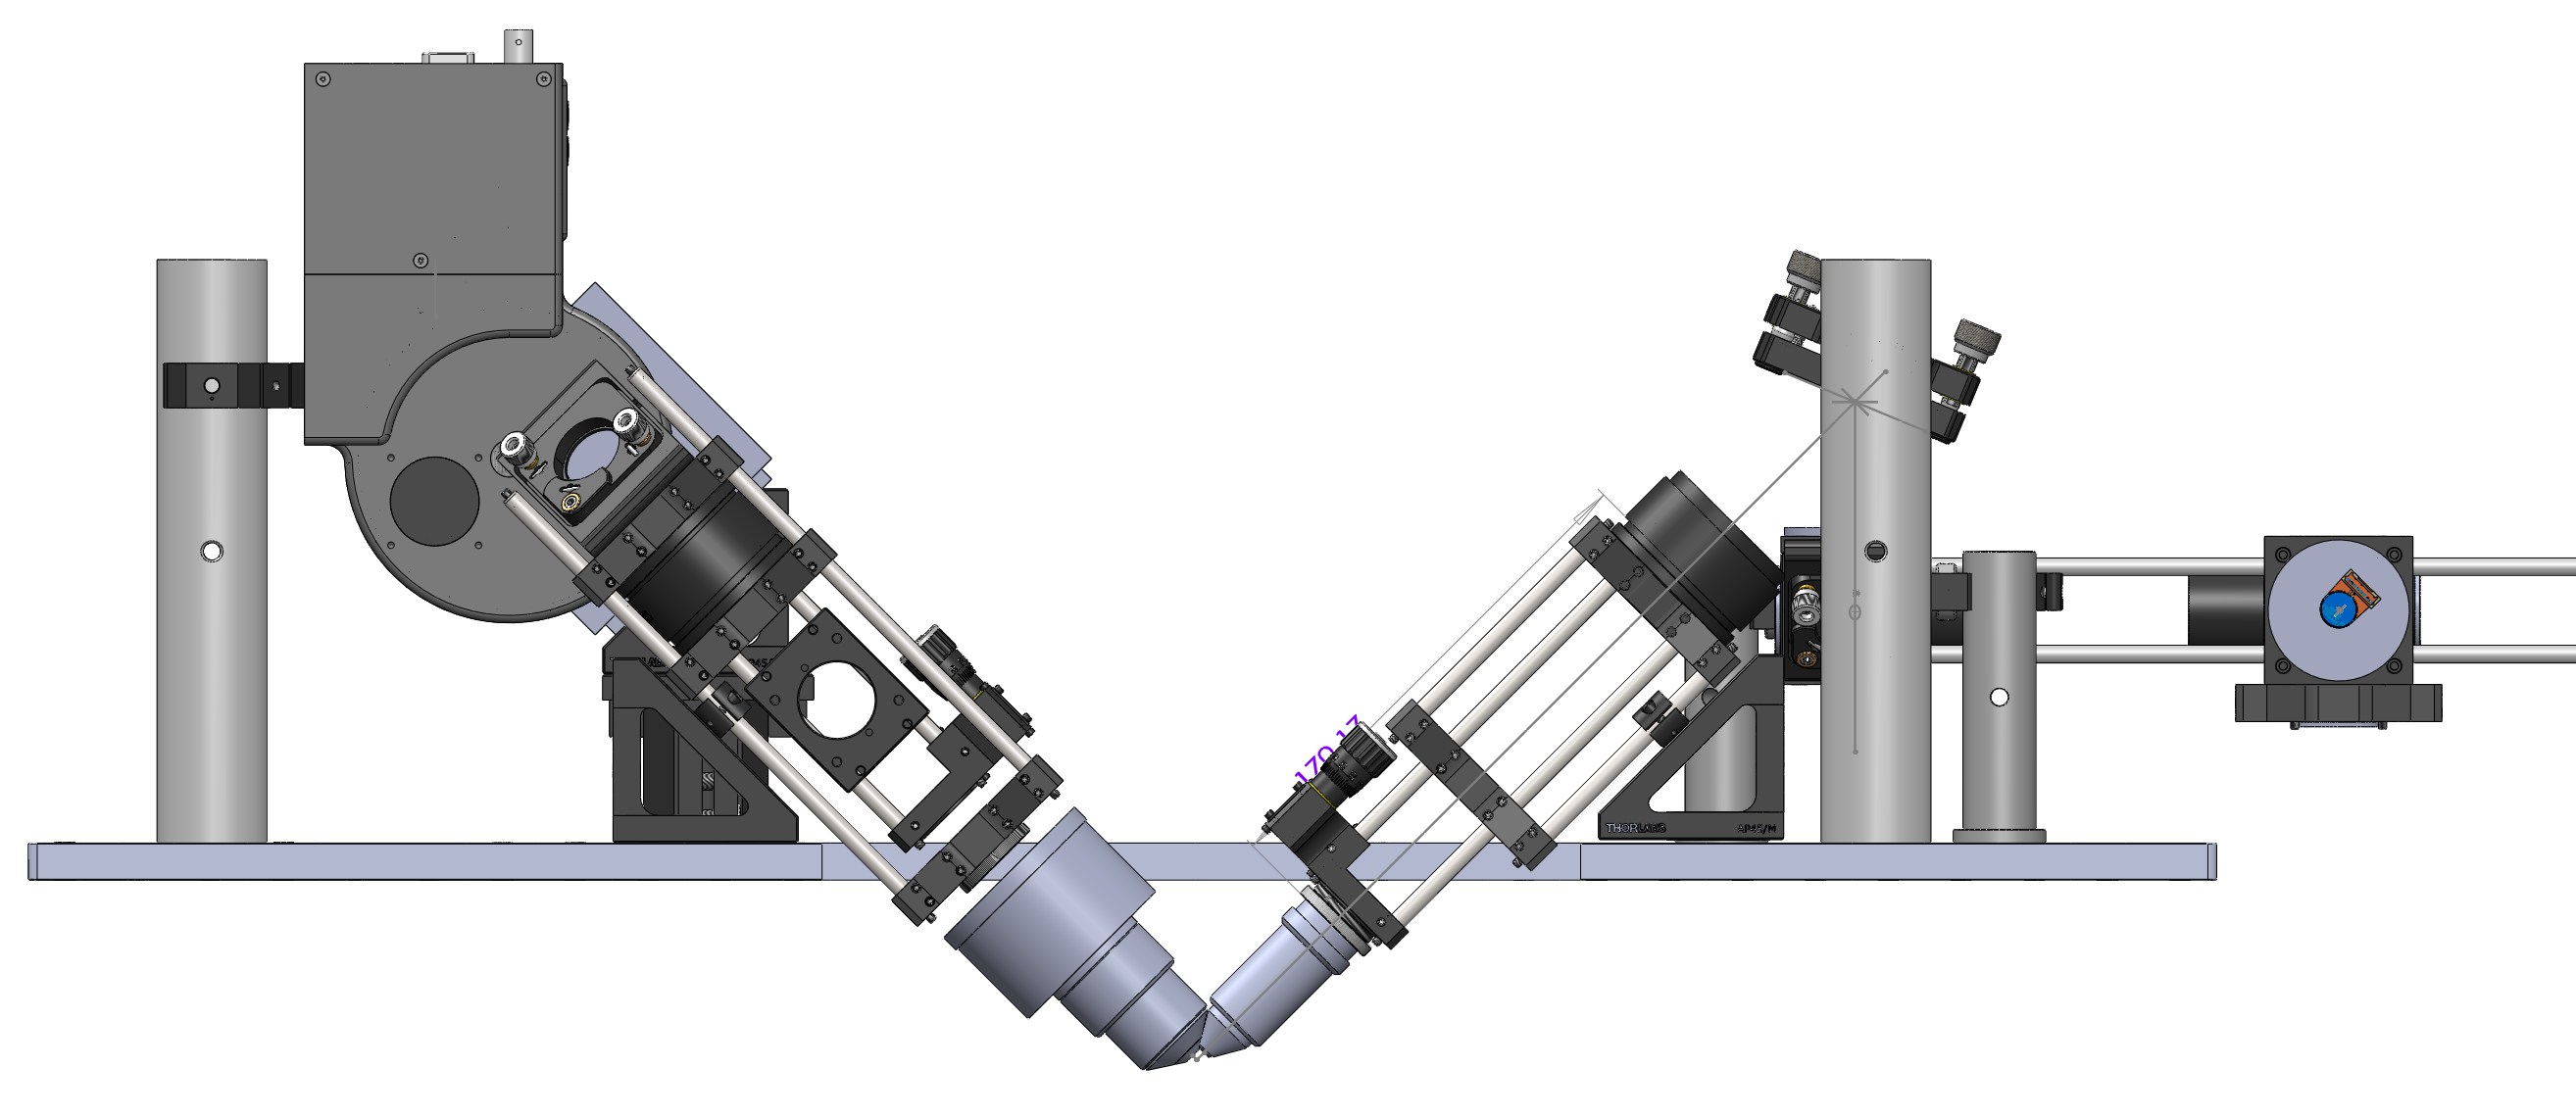
\includegraphics[width=1\linewidth]{./Raster/solidworks_design_front}
% \caption[CAD design of the \SI{45}{\degree} detection and illumination]{}\label{fig:solidworks_design_front}
% \end{figure}
%
% \begin{figure}
% 	\centering
% 	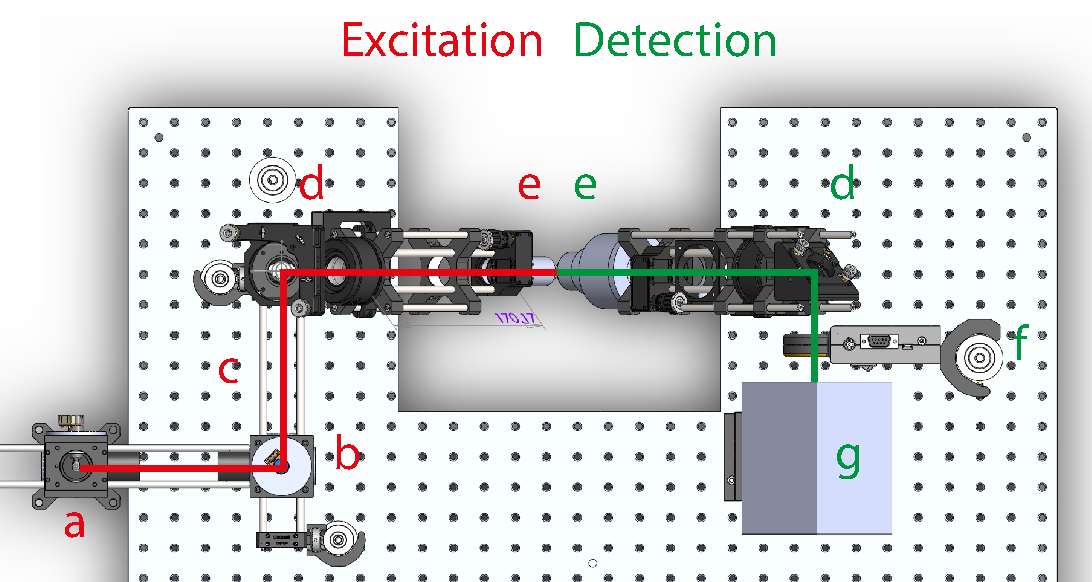
\includegraphics[width=\linewidth]{./soldiworks_top}
% 	\caption[Top down schematic of SPIM]{
%     (a) Scan mirror which creates the \gls{light-sheet}.
%     (b) Scan mirror in \(z\) for scanning volumes.
%     (c) Position of telecentric lens.
%     (d) Tube lens \emph{ITL200}
%     (e) Objective lenses, with green having an objective actuator.
%     (f) Emission filter wheel
%     (g) sCMOS camera
%     }\label{fig:soldiworks_top}
% \end{figure}

% \subsubsection{Scan Lens}
% %TODO something
% The scan lens was characterised (See appendix \ref{appendix:scanlens}) and placed at ... %TODO
% %See Appendix

\subsubsection{Light-sheet shaping} %Edited

% \newacronym{FOV}{FOV}{Field of View}
% \newacronym{sCMOS}{sCMOS}{scientific Complementary Metal-Oxide-Semiconductor}
% \newacronym{NA}{NA}{Numerical Aperture}

Using the Orca Flash v4 camera (with a sensor size of \SI[product-units=repeat]{13x13}{\milli\meter}) and a detection objective magnification of \SI{25}{\times}, produced a \gls{FOV} with an extension of
% a required \acrshort{FOV} of
\SI{520}{\micro\meter} in the \(x\) and \(y\) directions.
To match the confocal width of the illumination beam to the \gls{FOV} of camera sensor the illumination required \SI{0.15}{}~\gls{NA} at the back aperture of the illumination objective for \SI{561}{\nano\meter} light; providing a beam waist (\gls{light-sheet} thickness) of \SI{1.3(1)}{\micro\meter}, from Equation~\ref{eq:Rayleigh}.
%\acrshort{NA}
To create an \gls{NA} of \SI{0.15}, for an objective of focal length \SI{20}{\milli\meter}, the back aperture would need to be filled by a beam of diameter \SI{6}{\milli\meter}.

Using an \emph{ITL200} tube lens with a \emph{Nikon A1} scan lens provided \SI{5.37}{\times} magnification (See Appendix~\ref{appendix:scanlens}), meaning the illumination objective back aperture would have been overfilled (\SI{7.52}{\milli\meter} beam diameter at the back aperture) and the usable \gls{FOV} too small.
To address this, an iris was placed at the back aperture of the illumination objective to allow for manual tuning of the \gls{NA}.
The downside of stopping down the back aperture, was that some light was discarded
\Gls{light-sheet} systems do not require large doses to function (\SI{\sim1}{\milli\watt}) and discarding a fraction of the light from the \SI{100}{\milli\watt} sources was not found to impede imaging.

%With a scan lens focal \SI{37.3\pm0.1}{\milli\meter}

%In the old SPIM a standard NA of laser used was 0.15 which created a FOV of \SI{520}{\micro\meter} \footnote{The chip size of the sCMOS camera is \SI{13}{\milli\meter} and the magnification of the detection objective lens is \SI{25}{}$\times$ giving a field of view of \SI{520}{\micro\meter}} and a beam waist of \SI{1.3 \pm 1}{\micro\meter} (from equation \ref{eq:rayleigh}).
%To recreate a numerical aperture of \SI{0.15 \pm 0.05}, for an objective of focal length \SI{20}{\milli\meter}  the back aperture would need to be filled by a beam of diameter \SI{6}{\milli\meter}.
%Therefore the illumination laser needs to be magnified \SI{1.7}{}$\times$.
%Standard optical lenses are heavily quantised in terms of their focal length, a viable magnification for instance would be a \SI{160}{\milli\meter} , \SI{30}{\milli\meter} pair placed just before the flip mirror.
%A very sensible use of lenses would involve exploiting the lens that conjugates the SLM to the image plane, provided the lens were placed after the flip mirror and not before, which is possible if the focal length of the SLM is set higher than \SI{330}{\milli\meter} and therefore placed after the flip mirror.

%The beam waist was measured for one colour though each colour may require its own additional lenses as well as the overall demagnifying telescope.
%These additional lenses directly after the laser heads would compensate for any width and colour dependent variances in the field of view of the light sheet; the gratuitous additional optics (six lens for three uncorrected colours) may make this solution inviable as the only correction it will achieve is likely a small improvement in light sheet homogeneity.

\subsection{Detection}

%The optics surrounding the detection arm are far simpler than the excitation arm.
A PlanAchromat \SI{25}{\times} high (\SI{1.1}{}) \gls{NA} objective was used as the detection lens, owing to its excellent lateral resolution, unparalleled for a water dipping lens, and to its suitability to the mechanical constraints of the \gls{light-sheet} system.
This was coupled to a second \emph{ITL200} tube lens which imaged infinity corrected emission light onto the Orca Flash 4.0v2 detector.
% Before the detector there was
In the path between the detection objective a Prior Filter wheel housing emission filters (Semrock the \emph{442/647};
Chroma the \emph{ET605/70m} and \emph{ZT405/488/561/647rpc}) was installed to reject scattered illumination light.
%The emission filter is used to reject excitation light scattered from the sample, though this signal should be weak it is very difficult to correct for this digitally and so the filters are necessary.
%\subsubsection{Parfocal relay}

A further lens relay was added on the \gls{imaging optical rail} after the \gls{detection arm} turning mirror.
The relay comprised a tube lens and two objective lenses on a rotating turret.
This provided a par-focal solution for magnifying the imaging by \SI{2.5}{\times} (\emph{Olympus MPLFLN1.25x}) and \SI{1.25}{\times} (\emph{Olympus MPLFLN2.5x}) for \SI{62.5}{\times} and \SI{31.25}{\times} total magnifications respectively.
Using microscope objectives for the additional optical relay ensured that there were minimal optical losses as the lenses are designed for the weak fluorescent signal, as well as for minimal distortion and chromatic aberrations.
%Imaging at \SI{62.5}{\times} magnification gives \SI{99.2}{\nano\meter} lateral sampling at the specimen plane.
The \glslink{Rayleigh length}{Raleigh} condition of the system, using \SI{561}{\nano\meter} light, is \SI{311}{\nano\meter} resolution.
%Meaning that
Therefore, at \SI{62.5}{\times} magnification, the system is sampled sufficiently for \glslink{nyquist sampling theory}{Nyquist criterion} (\SI{155.55}{\nano\meter})
%\footnote{which states that the sampling of a system needs be twice the bandwidth of a band-limited signal}
as the demagnified width of each \gls{photosite} (from the camera, at the specimen plane) is \(\frac{\SI{6.5}{\micro\meter}}{62.5}=\SI{104}{\nano\meter}\).

% under Nyquist sample criteon
%\section{Control}
\section{Software}

To control the \gls{light-sheet} microscope and acquire imaging data an open-source~\cite{russellSpimcontroller2017} software interface was developed, using \gls{LabVIEW}, to
% needed which would
send the appropriate electronic signals and serial commands.
%\subsubsection{Control}

\begin{figure}
    \centering
  \includegraphics{./controller_scheme} %TODO my own.
  \caption[Control schematic of the digitally scanned light-sheet microscope]{
  Control schematic of the digitally scanned light-sheet microscope.
  All control signals are generated within \gls{LabVIEW} and distributed to the components.
  Components requiring fast signalling (lasers, scanning mirror, objective actuators) are synchronised by sending pre-built packaged signal trains.}\label{fig:control}
\end{figure}

% Comntrol schematic illustrator.

%We controlled this like that and here is a schematic of how it all connects:

\subsection{Signalling} %Edited slightly?

%\subsection{Implementation}
%Talk about synchornisaiton
Precise synchronisation is needed for confocal slit-scanning (Chapter~\ref{chapter:dualslit}) to be viable, as the time between the switching of active \gls{photosite} rows at \SI{100}{\hertz} for the Orca Flash v4 is \SI{\sim10}{\micro\second}. %TODO justify this better than surprise confocal?
%In the light-sheet system used here, t
This was achieved using fast electronics to send sets of packaged voltage waveforms through a National Instruments \gls{DAQ} module.
Once a \gls{TTL} 5V signal is sent to the camera, there is a delay of approximately \SI{10}{\milli\second} for the electronics to initialise on the camera.
During this window the \(y\) mirror, which creates the \gls{light-sheet}, and \(z\) mirror are pre-driven so that the mirrors are travelling at a constant velocity during the exposure window, giving a uniform illumination.
The time-point of the start of the exposure window was found empirically (\SI{9.8}{\milli\second} after camera triggering) by tuning this window until the illumination profile, under slit scanning, was uniform when visualised using fluorescent dye (Rhodamine).
During the exposure, a \gls{TTL} signal is sent to the requisite laser channel for illumination.
Once the exposure window is finished, the \(y\) and \(z\) mirror is sinusoidally returned to the start voltage for the next exposure (see \figurename~\ref{fig:slit_signals}); sinusoidal ramping helps protect the mirror against inertia-induced damage.

\begin{figure}
  \centering
  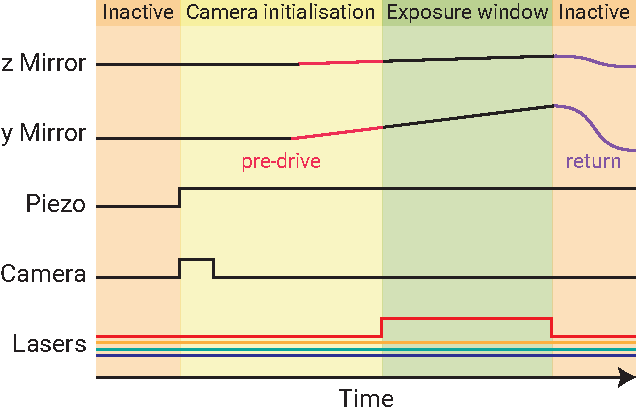
\includegraphics{slit_signals}
  \caption[The signals required to synchronise a rolling shutter in a digitally scanned light sheet]{
  The signals required to synchronise a rolling shutter in a digitally scanned light sheet.
  A pre-drive phase for the \(y\) mirror is needed to ensure the illumination profile of the light-sheet is uniform.
  The camera requires time to initialise the electronics and so a delay period is added within which the pre-drive of both mirrors is performed.
  Both mirrors are sinusoidally returned to their start position ready for the next acquisition.
  }\label{fig:slit_signals}
\end{figure}

Control and synchronisation of the filter wheel and XYZ translation stage was achieved using \gls{RS232} serial commands, as precise timing was not needed and direct feedback on the status of the stage and filter was desirable. %from the controller on where the stage and Filter

%TODO Basic overview.
%Sample Area
%	Requirements and Limitations of the samples to be used
%Illumination
%
%Detection
%Image Acquisition
%	Hardware interfacing, software control and end-user interface

%\subsection{Image Acquisition: Software Design}

%TODO discuss aims of software and version control

\subsection{\gls{LabVIEW} control software}

A modular, extensible and easy-to-use software solution was needed to control the \gls{light-sheet} microscope.
\gls{LabVIEW}, a graphical programming language with an emphasis on electronic systems control, was used.
\gls{LabVIEW} provides a wide library of drivers and libraries for interfacing; in particular the Orca Flash v4 has \gls{LabVIEW} drivers for direct control of its reader functionality, including the requisite commands for confocal slit scanning.

\subsubsection{\gls{LabVIEW} architecture}

% LabVIEW is a graphical programming software package designed to produce simple, modifiable, user-friendly software in science.
% LabVIEW provides a wide library of drivers and libraries for hardware interfacing in science.
% Due to LabVIEW's modularity and fast development environment it is ideal for producing software for a microscope under development as any new hardware can be quickly and easily implemented and not necessarily by the original software writer.

It was required that the components within the microscope were interfaced with in a parallel manner, as well as being able to control and interface with each other (e.g.~the XYZ controller triggering the capturing of an image volume).
The software controller was engineered using a \gls{producer-consumer architecture} where each \glslink{producer-consumer architecture}{consumer} was a parallel \gls{state machine}.
The \glslink{producer-consumer architecture}{producer} received front panel inputs, then converted and passed those commands on to the \glslink{producer-consumer architecture}{consumer}s.
Using a \gls{queueing architecture} ensured that command flooding and \gls{race conditions} were avoided, and the consumer loop was self-regulating.
%This ensures that command flooding and race conditions are avoided and the consumer loop can be self regulating.

The commands were packaged as a bundle.
The first part being an enumerated type which changed the \emph{state} of the \glslink{producer-consumer architecture}{consumer}; the second being the necessary front panel data which informed the consumer on any updates to the states (e.g.~camera exposure).
By using this queuing architecture, consumers can then communicate with each other whilst functioning independently.

%
% %A well planned, modular and user-friendly interface is very important whenever creating hardware-user interfaces.
% %In the case of the new microscope this software needs three different components.
% %The first is t
% The software needed to several modules: the Camera control software, which controls the detection arm of the microscope, needed to
% %; this software needs to
% allow a user to save two and three dimensional stacks of images and still be accessible to change and upgrade as more and difficult biological questions were to be addressed.
%
% A XYZ stage controller controller for the stage which that could interface with the camera software (to take images for large area scanning for instance)%. as well as being user friendly enough to accurately control the XYZ stage.
% and finally, a waveform generator to control and synchronise the scanning mirrors, focus piezo and potentially tunable lenses.
% These software also needed to be designed as modules so that a user could use each independent of the others.
% To satisfy these criteria LabVIEW was chosen as the programming environment to be used.

%\subsubsection{Camera module}


% \subsubsection{Queuing}
%
% When interfacing with hardware a key challenge programmers face is how to mitigate command flooding at the device.
% A user may for instance want to send several commands in a linear fashion, but the device may only be able to successfully implement one or none if it crashes with overload or misinterprets the command as it is processing another.
% LabVIEW offers a queueing architecture where a programmer can send a command into a queue which will operate something, be it a real device or a construct within the software.
% This queueing opens a myriad of possibilities.
% The programmer can not only queue an infinite line of commands but also remove duplicate commands, truncate a command queue, change the routine of operation to a first in first out (FIFO) routine rather than first in last out (FILO) or even enforce that only one command can exist it the queue at any time.
%
% \subsubsection{Simple State Machine}
%
% A state machine is a fundamental computing architecture which can contend with a great deal of complex programmatical challenges.
% A common example of a state machine is a vending machine: when left alone the vending machine keeps its state (usually an enumerated variable) as idle.
% If a user adds a coin it begins a routine of \textit{add currency to running total}.
% If a user presses dispense the next state will check the running total of currency, if the currency is too low the current state then changes its next state to return coin or any other operation.
% It is a very simple method of keeping a clear routine within the program rather than any abstractions that would occur if programmed otherwise.
%
%
% \subsubsection{Producer Consumer}
%
% %In LabVIEW the combination of queueing and state machines facilitates the producer consumer concept, whereby the producer is an independent parallel routine which can queue commands for a consumer.
% %The most simple template for this is an event driven producer recommended as the start of any LabVIEW routine, whereby the event loop collects commands from the Graphical User Interface (the front panel in LabVIEW).
% %This producer then produces commands to be sent to the consumer loop which processes them.
% This ensures that command flooding and race conditions are avoided and the consumer loop can be self regulating.
% Crucially, queued commands can come from more than one entity in this style of environment.
% Not only can commands from the front panel control the consumer, but also commands (if correctly written) can arrive from sources such as the internet, other devices, or other front panels within LabVIEW.

% \begin{figure}
% \centering
% 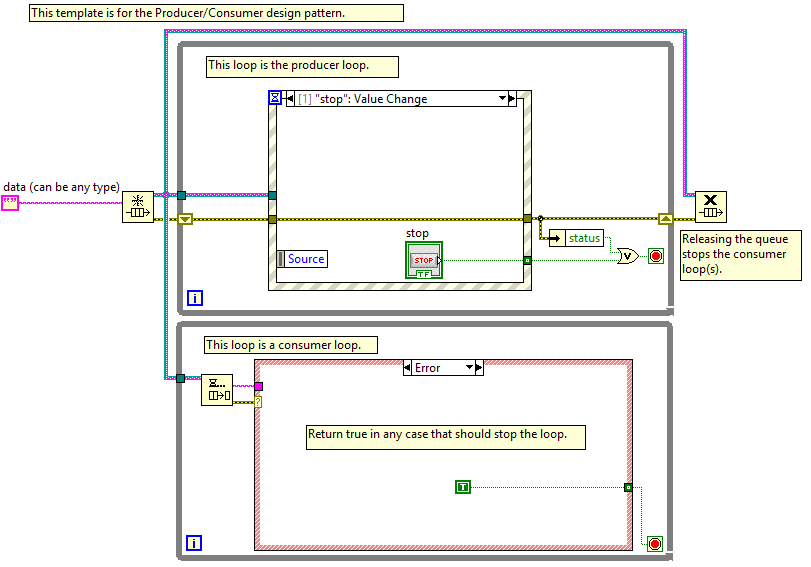
\includegraphics[width=0.8\linewidth]{Figures/standard_pro_cons}
% \caption[LabVIEW Producer Consumer Template]{A producer consumer template provided by national instruments.
% The top loop is an event driven (user front panel input) producer loop, the bottom loop consumes these commands and acts accordingly.}
% \label{fig:standard_pro_cons}
% \end{figure}

\begin{figure}
    \centering
    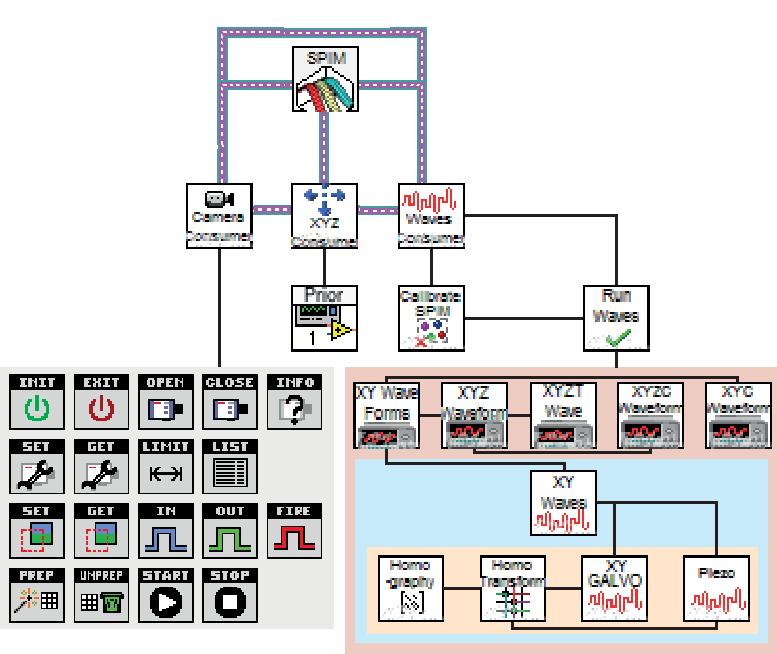
\includegraphics{/software_layout}
    \caption[Schematic diagram of the dependancies of each routine in the \gls{LabVIEW} software (\emph{SPIM}, the kernel) that runs the light-sheet microscope]{
    Schematic diagram of the dependancies of each routine in the \gls{LabVIEW} software (\emph{SPIM}, the kernel) that runs the light-sheet microscope.
    The \emph{Camera consumer} and \emph{XYZ consumer} package the Hamamatsu capture (grey) and Prior iScan libraries (\emph{Scan}) respectively.
    The \emph{Waves consumer} packages the signal generating routines (red) and drives the resultant signals to the DAQ board using \emph{Run waves}.
    Each of the waves routines (red) are concatenations of \emph{XY waveforms}, which itself relies on \emph{XY waves} (blue) generates signal trains from calibration coordinates and front panel data.
    \emph{Homo-graphy} and \emph{Homo transform} (orange) take calibration coordinates to then inform \emph{XY Galvos}.\\
    The purple connections represent \gls{LabVIEW} queue connectors; each purple-connected module, other than the main kernel (SPIM), was an independent queued consumer state machine.
    State changing commands were added to each module's queue and could be received from any other connected module.
    This allowed for conditions such as the \emph{XYZ controller} being able to request \emph{Camera consumer} for an image or volume to be recorded using a simple \glslink{enumerated type}{enumerated} command.
    }\label{fig:software_layout}
\end{figure}

\subsubsection{Kernel}

The kernel stores the acquisition settings and initiates all the queues to be sent the sub modules, \textbf{Camera}, \textbf{Waveform Generator} and \textbf{XYZ Translator}.
All acquisition settings and properties are converted into \gls{enumerated type}{enumerated} state machine commands.
Acquisition modes are organised into imaging orders, such as \emph{XYZ}, \emph{XYZC}, \emph{XYCZ}, \emph{XYT}; where \emph{XY} is a single frame, \emph{Z} is an iteration axially, \emph{C} is the colour channels selected, and \emph{T} is the time course selected.
Each of the dimensions (\emph{XYZT}) are governed by the parameters \emph{Start}, \emph{Step}, \emph{Range}; where start is the initial position or time; step is the step size, meaning spatial resolution or temporal resolution; and range is the range over which the dimension covers, spatially or temporally.
For colour, a \(2\times n\) array of enumerated typed is constructed for laser line and respective filter wheel position choice.
The kernel also stores the calibration coordinates (see Chapter~\ref{chapter:homography}) sent from the calibration module.
All of the
%these
settings can then exported as XML files and may be reloaded later.
%The kernel also manages the saving and loading of acquisition settings.


\subsubsection{Camera module}

The camera module consists of two consumers.
The first
% module runs a
consumer initiates and destroys the camera communications; as well as
%There are also
soft update states (for instance changes to \gls{exposure time}), and hard update states
(for when an acquisition setting requires the camera link to be unloaded, such as changing the \emph{sensor mode} which controls the shutter directions).
The difference between hard and soft updates is poorly documented and the categorisation of was found empirically.

The second consumer loop exists within the camera module to handle saving and displaying of image data.
This consumer has two settings: the first receives queued image arrays directly from the camera, this is used for live preview mode and small image sequences such as single volumes; the second reads and converts image files from the file-stream of the camera.
The latter mode does not drop frames as the camera is streaming data directly to the hard drive, provided the read and write streams of the hard-drive do not overflow.
The single frame acquisition mode will also not drop frames due to their sequence being queued, but, there may be a delay between the presented image and the live view at high frame rates.

\paragraph{Virtual slit}
%{Virtual slit}

The virtual slit for confocal slit scanning was addressed in the camera's hardware directly using hex address \(\times 400210\).
Mode 1, sets the camera to full frame and mode 12, slit scanning.
Once the mode is set the line interval (\(\times 403850\)) and slit exposure (\(\times \text{1F0110}\)) is set according to the equation:

\begin{align}
    \text{Slit exposure} &= \frac{\text{Exposure} \times \text{Slit width}}{\SI{10}{} + \text{FOV}_y + \text{Slit width}} \\
    \text{Line interval} &= \frac{\text{Slit exposure}}{\text{Slit width}}
\end{align}

\subsubsection{Waveform module}

The waveforms module handles all signalling for the \gls{DAQ} board (four laser lines, piezo, Y mirror, Z mirror, camera trigger, filter wheel).
The waveforms are constructed from the acquisition settings %for digital and analogue signals, which
and are forced to synchronise using propagation error values
\footnote{\gls{LabVIEW} is a data flow language so synchronisation is controlled using propagating variables and commonly using the error output of the function.}
.

The camera and lasers were addressed using digital (\gls{TTL}) signals which are hardware limited between \SIrange{0}{5}{\volt}.
Voltages to the objective actuator and scanning mirrors were software limited between \SIrange{0}{10}{\volt} (\SI{10}{\volt} = \SI{100}{\micro\meter}) and \SIrange{-10}{10}{\volt} respectively, to prevent damage to the electronics.
The objective actuator was positioned linearly, by voltage, using the conversation \SI{10}{\per\volt\micro\meter}; with \SI{16}{\bit} voltage resolution from the \gls{DAQ}, this gave an addressable axial resolution of \SI{1.52}{\nano\meter}, which was \SI{4}{\times} larger than the reported closed loop resolution (\SI{0.4}{\nano\meter}) of actuator.
Achieving the full resolution would have required addressing the actuator using serial commands which would have been too slow for the required imaging modes, such particle tracking.
As such the resolution trade-off was accepted.


%  with the digital.
%To create the wavesforms, XY wavefroms are concantThe waveforms are generated by concatenating
%
% \subsubsection{XYZ stage and filter wheel module}
%
% The XYZ module reads and writes XYZ stage positions and filter wheel positions using \gls{RS232}.
% For imaging, a list of locations to tour was added with the ability to the trigger current kernel acquisition mode in the kernel at each location visited.

\subsubsection{Calibration module}

The calibration module set the microscope to live image preview mode with direct user control over the objective actuator voltage and mirror voltages.
The module was used to set the limits of the usable volumetric \gls{FOV} and match the focus of the objective to mirror positions; this is discussed in detail in Chapter~\ref{chapter:homography}.
%
% \clearpage
% \begin{figure}
%   \centering
%   \begin{subfigure}[t]{\textwidth}
%     \centering
%     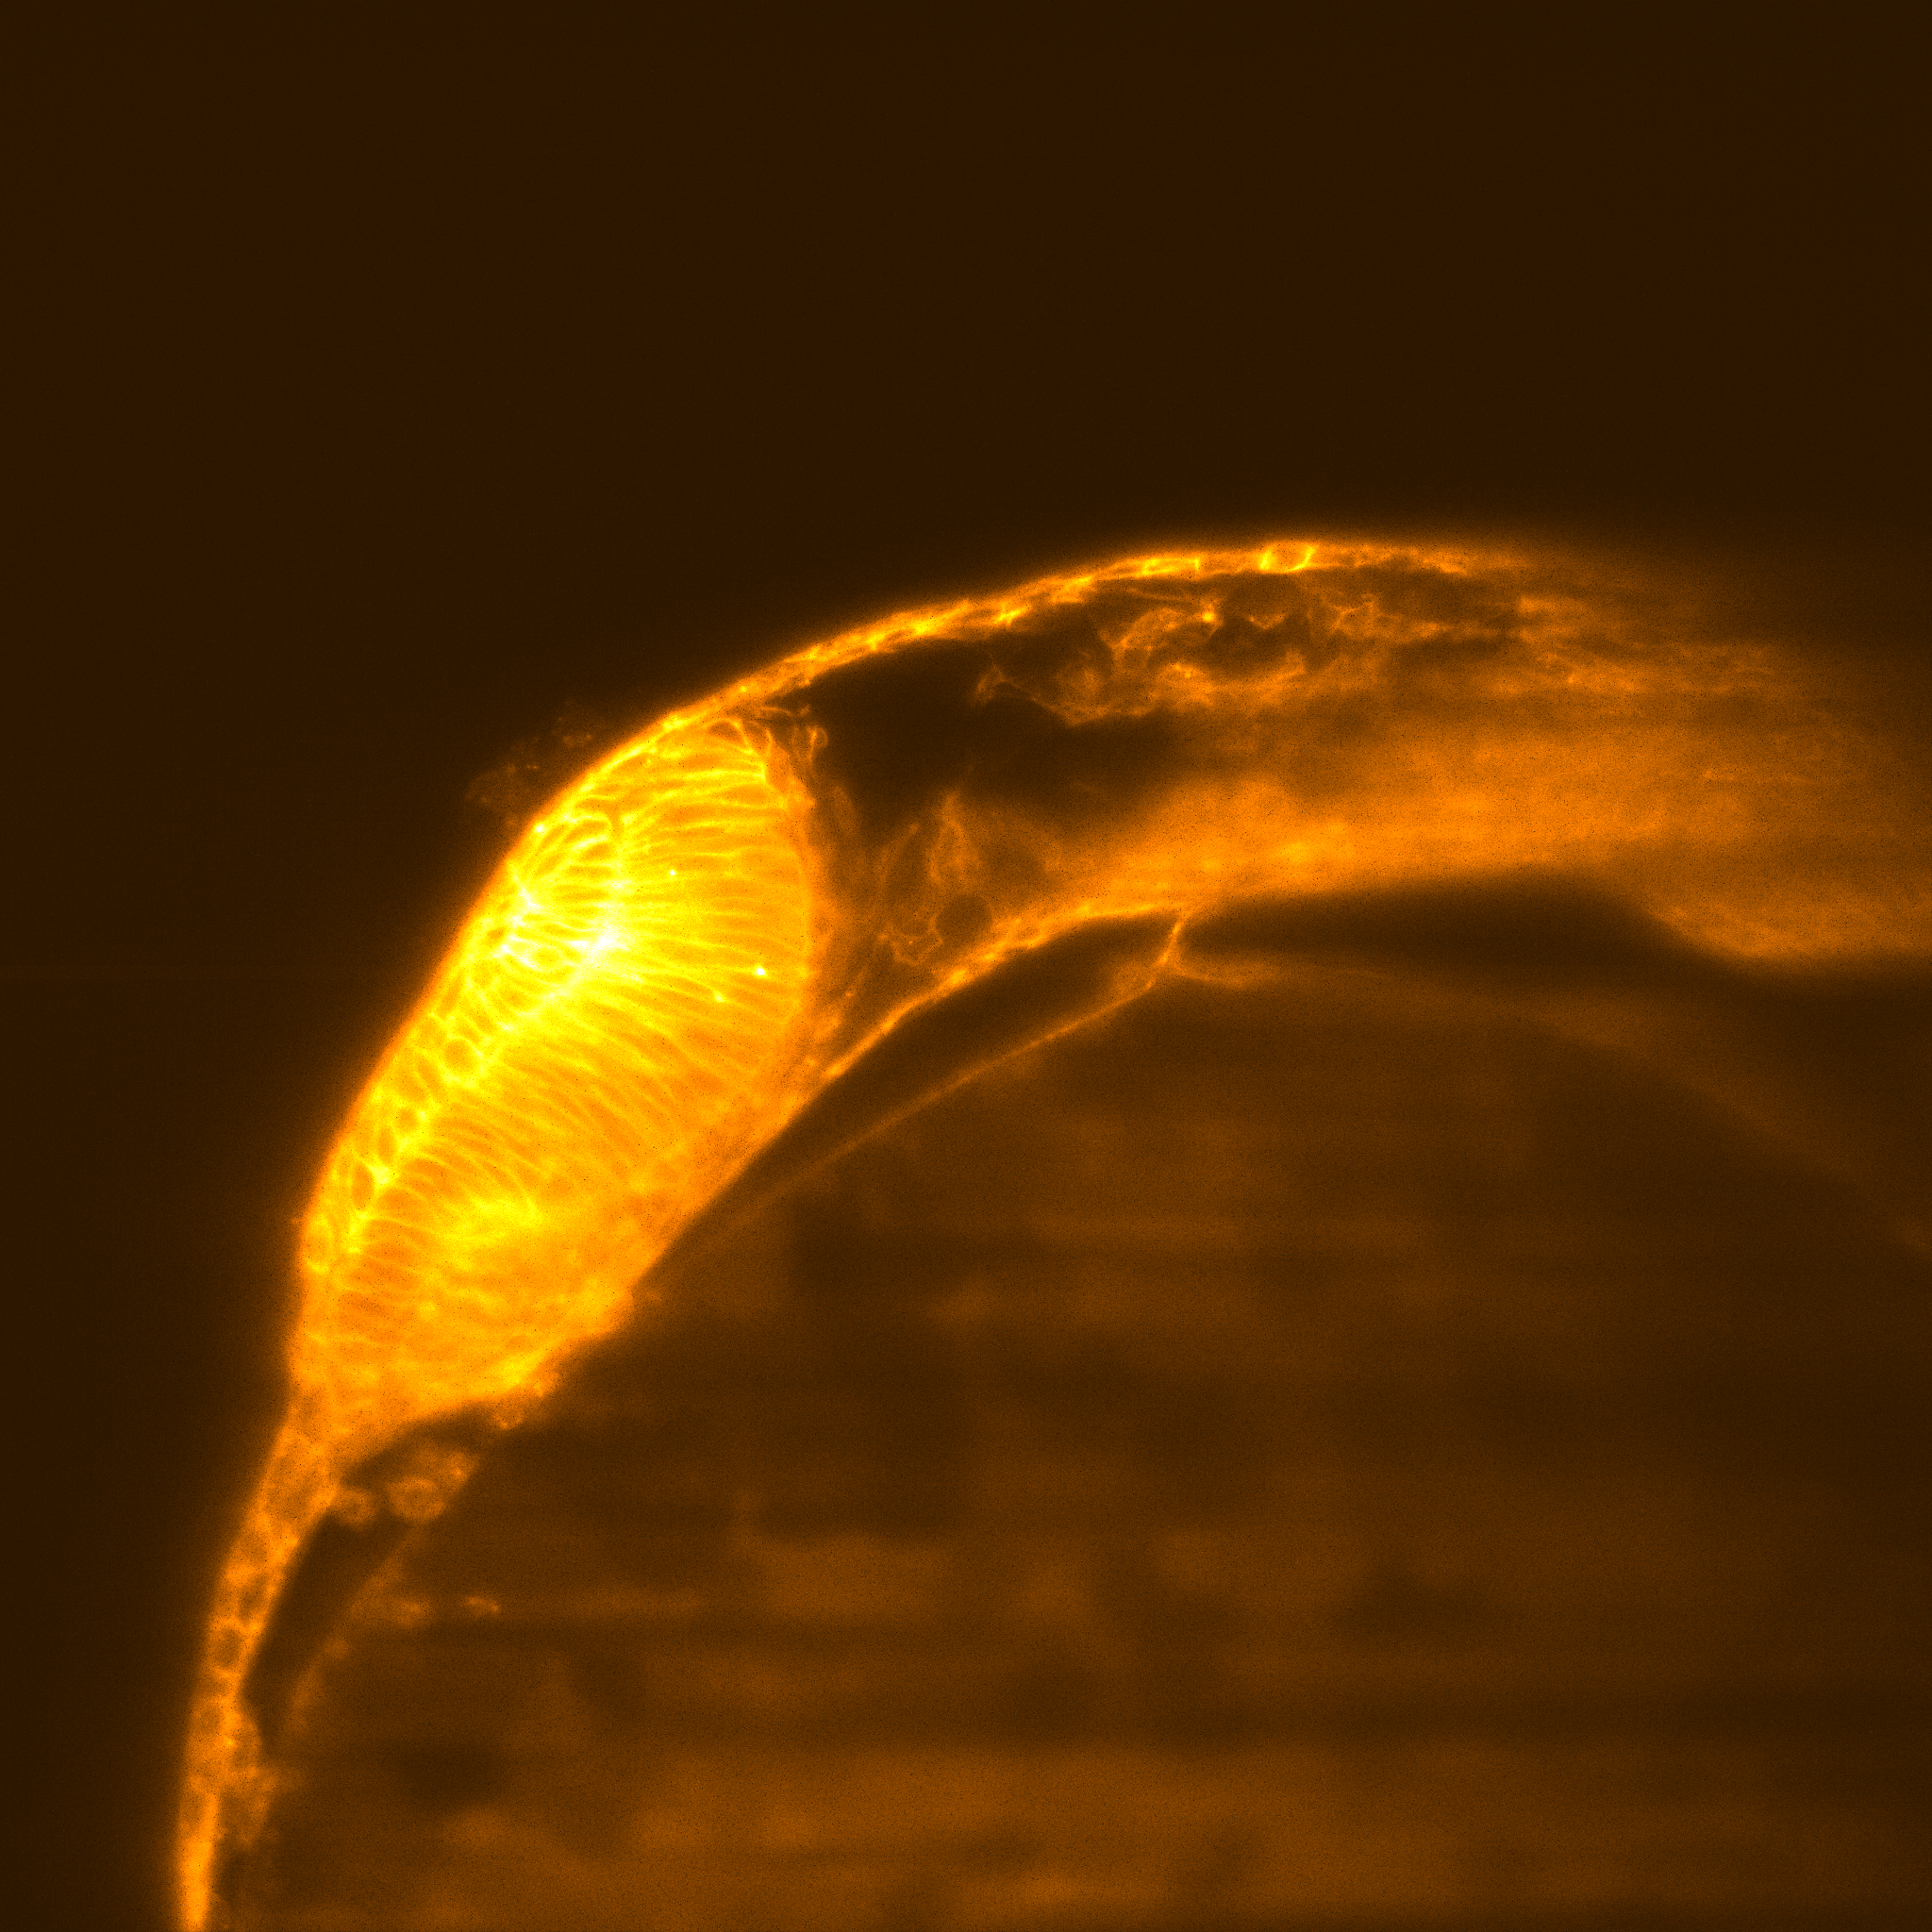
\includegraphics[width=\textwidth]{zfish_48hr_eye_magneta}
%     \caption{\SI{48}{\hour}, \gls{zebrafish} eye}
%   \end{subfigure}
%   \caption[Preliminary images of zebrafish]{Preliminary images of zebrafish expressing \gls{GFP} and produced from the light-sheet microscope designed and built in this work.}\label{fig:zfish_pretty}
% \end{figure}
%   \clearpage
%   \begin{figure}
%   \ContinuedFloat{}
%   \begin{subfigure}[t]{\textwidth}
%     \centering
%     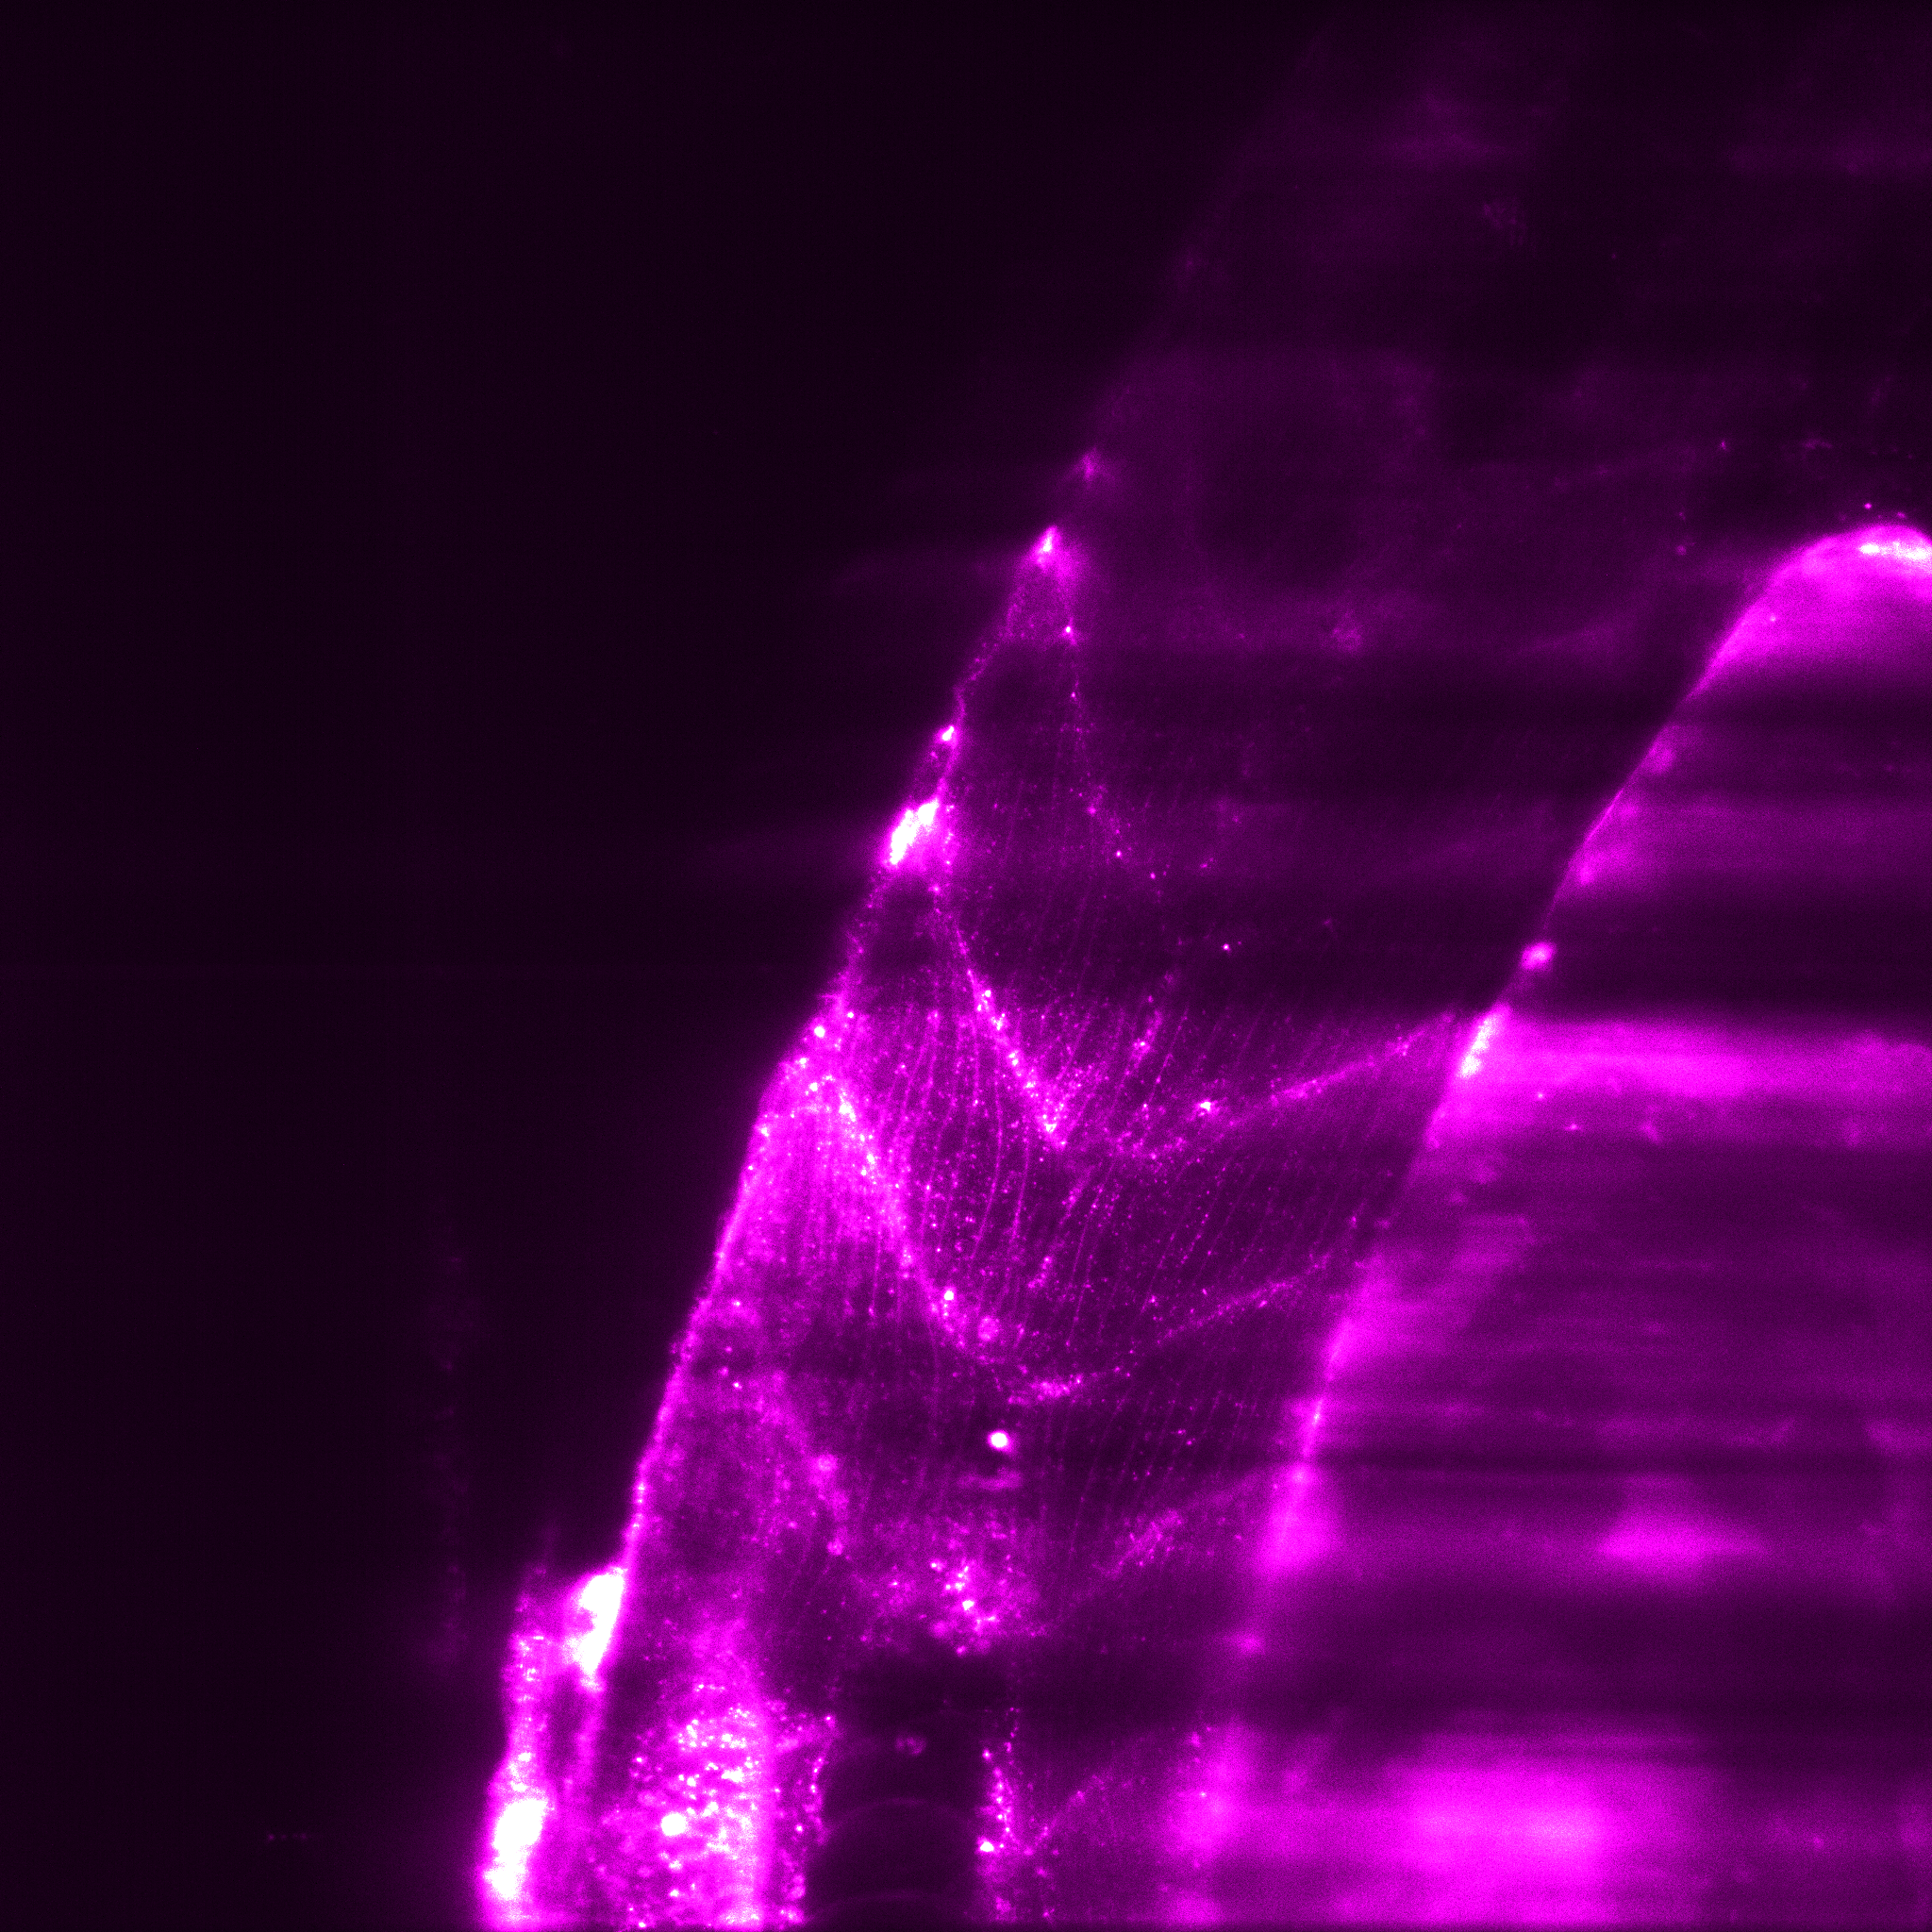
\includegraphics[width=\textwidth]{zfish_48hr_noto_magenta}
%     \caption{\SI{48}{\hour}, \gls{zebrafish} notochord}
%   \end{subfigure}
%     \caption{}
% \end{figure}
% \clearpage
% a double-page figure
\begin{figure}[p]% will be the left-side figure
  \begin{leftfullpage}
    \centering
    \begin{subfigure}[t]{\textwidth}
      \centering
      \includegraphics[width=\textwidth]{zfish_48hr_eye_magneta}
      \caption{\SI{48}{\hour}, \gls{zebrafish} eye}
    \end{subfigure}
    \caption[Preliminary images of zebrafish]{Preliminary images of zebrafish expressing \gls{GFP} and produced from the light-sheet microscope designed and built in this work.}\label{fig:zfish_pretty}
  \end{leftfullpage}
\end{figure}
\begin{figure}[p]% will be the right-side figure
  \begin{fullpage}
    \ContinuedFloat{}
    \begin{subfigure}[t]{\textwidth}
      \centering
      \includegraphics[width=\textwidth]{zfish_48hr_noto_magenta}
      \caption{\SI{48}{\hour}, \gls{zebrafish} notochord}
    \end{subfigure}
      \caption[]{\phantom{.}\linebreak\phantom{.}}
  \end{fullpage}
\end{figure}
% end of the figure

% \begin{figure}
%   \begin{leftfullpage}
%     \centering
%     \begin{subfigure}[t]{\textwidth}
%       \centering
%       \includegraphics[width=\textwidth]{zfish_48hr_eye_magneta}
%       \caption{\SI{48}{\hour}, \gls{zebrafish} eye}
%     \end{subfigure}
%     \caption[Preliminary images of zebrafish]{Preliminary images of zebrafish expressing \gls{GFP} and produced from the light-sheet microscope designed and built in this work.}\label{fig:zfish_pretty}
%   \end{leftfullpage}
% \end{figure}
%   \begin{figure}
%     \ContinuedFloat{}
%       \begin{fullpage}
%     \begin{subfigure}[t]{\textwidth}
%       \centering
%       \includegraphics[width=\textwidth]{zfish_48hr_noto_magenta}
%       \caption{\SI{48}{\hour}, \gls{zebrafish} notochord}
%     \end{subfigure}
%       \caption{}
%   \end{fullpage}
% \end{figure}


% \begin{figure}
%   \centering
%   \begin{subfigure}[t]{0.4\linewidth}
%     \centering
%     \includegraphics[width=0.9\linewidth]{zfish_48hr_eye_magneta}
%     \caption{\SI{48}{\hour}, \gls{zebrafish} eye}
%   \end{subfigure}\quad
%   \begin{subfigure}[t]{0.4\linewidth}
%     \centering
%     \includegraphics[width=0.9\linewidth]{zfish_48hr_noto_magenta}
%     \caption{\SI{48}{\hour}, \gls{zebrafish} notochord}
%   \end{subfigure}
%   \caption[Preliminary images of zebrafish]{Preliminary images of zebrafish expressing \gls{GFP} and produced from the light-sheet microscope designed and built in this work.}\label{fig:zfish_pretty}
% \end{figure}

\section{Specification review}

A \gls{light-sheet} microscope was built to the design specification in Section~\ref{sec:specification}.

\paragraph{\ref{item:volumes}. Fast volumetric imaging}
Fast volumetric imaging (see \figurename~\ref{fig:zfish_pretty}) was achieved using a pair of optically relayed scanning mirrors to rapidly sweep a virtual light-sheet through volumes.
A Piezo objective actuator was used to maximise the axial speed at which volumes could be acquired.

\paragraph{\ref{item:colour}. Multi-colour volumetric imaging}
Four laser lines were used with a 6-port fast filter wheel on the \gls{imaging optical rail} and
%the illumination lines were \gls{TTL} trigged diode lasers
simultaneous \gls{TTL}-control of diode laser illumination
to allow for fast colour switching, to image multi-colour volumes rapidly.
The limiting step for speed was the filter wheel, though multi-notch filters were used for bespoke cases needing maximal colour switching speed (in which case only the \gls{Laser} diodes were switched to change colour channels).% be used in bespoke cases

\paragraph{\ref{item:mounting}. Capacity for multiple methods of sample mounting}
An XYZ translator was mounted well below the two dipping objectives.
This allowed for traditional mounting strategies, such as agarose filled \gls{FEP} tubing, as well as bespoke solutions for difficult samples, such as live cells.
The translator enabled precision positioning as well as large FOV imaging through positional mosaicing.
Chapter~\ref{chapter:chamber} discusses, in detail, the sample mounting procedures used.

\paragraph{\ref{item:scales}. Multiple magnifications}
A par-focal relay using microscope objective lenses was inserted in the detection path to allow for two FOVs to be chosen from. This allowed for the imaging of a large gamut of biological samples, from the cell up to the organism.

\paragraph{\ref{item:illumination}. Options for exotic illumination development}
A beam splitter was placed on the lower optical breadboard before reaching the scanning mirrors above. Using flip mirrors and beam dumps enabled the option of a dual-beam, concomitant illumination or an exotic illumination from the SLM found on one of the arms.

\paragraph{\ref{item:software}. User-friendly and extensible software scheme}
\gls{LabVIEW} was used to create a modular system for the control software.
By using an appropriate architecture, as detailed above, modules could interact freely and run in parallel.
\\
The following chapter will expand on the signal generation presented in this chapter in an attempt to optimise and maximise co-planarity between the imaging and illumination planes.

%The software was designed such that it could be ported to other systems with minimal re-programming

%
% % %The Prior controller interfaces with software via an \gls{RS232} protocol.
% % %Provided with the stage is a library of routines within LabVIEW that package the correct \gls{RS232} commands in a LabVIEW friendly format.
% % %These were then incorporated into $XYZ\_Controller.vi$ producer consumer loop.
% % %This time however the stage controlling consumer loop was a slave to the consumer that handled front panel inputs.
% % %This was because the controller is cantered about the list of positions.
% % This list sends positional commands to the stage, but also requires functions such as: clearing the positional list; adding current position to the beginning or the end of the list; controlling the delay between positions and sending save image volume commands.
% %
% % For filter wheel control, \gls{RS232} commands were synchronsied with the \gls{TTL} triggers from the Waveforms module.
% % A small listening routine was written to intercept triggers sent to a false channel, these triggers were then converted to filter wheel positions.
% % The maximum settling time for non-adjacent filters is \SI{40}{\milli\second}, so a comparable delay was added into the imaging routine to compensate for filter switching.
% % \gls{RS232} commands require a comparable amount of time in handshaking, so attempting to check if the filter wheel was in the correct place before continuing would not be faster.
%
% % drop frames, but has the potential to
%
% % Camera modules
% % Saving to ram or harddisk. Involved another consumer slave to take queued images from the camera consumer-cum-producer.
% % The camera required an idle state so as not to hang when no commands had been sent
% % Hard and soft update states, for camera.
% %% Virtual slit
% % Hex values, 10 ms delay
% % Waveform modules
% % Synchronised waveform sending
% %
% % Image
% % XYZ Module
%
% %\subsection{Camera module}
%
%
%
% % Camera.vi was designed to be the main running loop of the software environment.
% % That said, all of its functionality has been designed so that each function could be addressed by properly accessing the queue named \textbf{Camera}.
%
% %\subsubsection{Front Panel}~
%
% % Care was taken to ensure that the user experience of the Camera.vi was well received and fundamentally simple.
% % A simple user experience can both necessitate the microscope to be used by a lay individual for simple exercises as well as allow experienced users to access more advanced aspects of the microscope.
% % % The imaging area of the Camera.vi was therefore set within a scalable box, so that setting on the left and image recording settings would shift away.
% % The settings on the left were organised into categorised tabs and initialised with camera defaults so that a complicated set up procedure is unnecessary.
% % See Figure \ref{fig:camera_frontpanel} for depiction.
%
% \begin{figure}
% \centering
% \includegraphics[width=\linewidth]{Figures/camera_frontpanel}
% \caption[Front Panel of Camera.vi]{Front panel interface of the Camera.vi routine.
% On the left is all the information and camera tools a user should need, tabbed into categories.
% At the bottom options to stop the program and open other supplementary programs.
% On the right an intensity histogram so the user can clearly see if the image being produced is making good use of the full dynamic range of the camera or to monitor if the camera is being saturated.}
% \label{fig:camera_frontpanel}
% \end{figure}
%
% % \subsubsection{Back Panel}~
%
% %The camera itself is split into three states: \textbf{init}alisation, \textbf{active} and \textbf{deinit}ialisation.
% %This structure was used so that collaborators could easily contribute as required.
% %Within \textit{active} the full producer consumer architecture runs.
% %The top loop typically seen as the producer takes all the front panel commands possible, passing the commands with any relevant numbers or information) in a bundled structure) to the camera control consumer loop.
% % %This loop then updates the camera as required and passes any images it received to a third slave loop which displays images as well as saving them to disk.
% % This secondary loop uses a limited queue so that is for any reason LabVIEW cannot handle the output of the camera then frames will drop when in preview mode to compensate.
% % Two disk saving modes were implemented in case of extreme uses of the camera.
%
% \begin{figure}
% 	\centering
% 	\includegraphics[width=\linewidth]{Figures/camera_init}
% 	\caption[Camera initialisation state]{Camera initialisation, standard settings to produce a default video output.}
% 	\label{fig:camera_init}
% \end{figure}
%
% % The first mode extracts camera data directly to a temporary file on the hard drive (a \SI{300}{\mega\byte\per\second}
% % solid state drive \SI{1}{\tera\byte}
% % raid, which is typically sufficiently quick for standard operations) in an proprietary format which is later decrypted by the slave loop in parallel to the camera loop producing the files.
% % Each temporary file contains a simple stack of images, designed such that each stack would be a full three dimensional scan of a volume.
% % To avoid overwriting, each temporary file was automatically named by a number with a six digit upper limit, far beyond the limitations of the hard drive capacity.
%
% \begin{figure}
% 	\centering
% 	\includegraphics[width=\linewidth]{Figures/camera_active}
% 	\caption[Camera active state]{Camera active, a three stage consumer producer architecture which passes commands from top to bottom.
% The top loop sends user commands to the middle loop which controls the active status and frame collection, the bottom loop then saves and processes the image data produced in parallel.}
% 	\label{fig:camera_active}
% \end{figure}
%
% % The second mode records camera data directly to the computer's RAM which has much faster write speeds but is more limited in capacity to \SI{32}{\giga\byte}
% % in the current machine.
% % \footnote{For the camera to interface with the older software which controls the waveform generation it needs to have the same LabVIEW environment.
% % Unfortunately the old code was written in \SI{32}{\bit}
% % LabVIEW with a Mathscript module that has no \SI{64}{\bit}
% %  option as of yet.
% % This means that the waveform generation software will need to be completely rewritten if the RAM writing record mode is ever fully needed; \SI{32}{\bit}
% % systems are limited to \SI{2}{\giga\byte}
% % RAM considering the camera can output \SI{600}{\mega\byte\per\second}
% % this would overfill very quickly.
% % That said, the record to harddrive function can run perfectly well in a \SI{32}{\bit}
% % environment.
% % Horses for courses.}
%
%
% % \paragraph{Virtual Slit}
% %
% % The \textit{Orca 4v2} has this slit scanning mode embedded in its firmware and is accessible from the supplied software.
% % Inducing this within LabVIEW requires sending values to specific hex addresses using \textit{advanced\_property} functions.
% % Two modes were implemented, a manual mode for debugging purposes, and an automated mode which reads the current input to create a suitably synchronised rolling shutter, see Figure \ref{fig:camera_virtual_slit_module}.
%
% \begin{figure}
% \centering
% \includegraphics[width=0.7\linewidth]{Figures/camera_virtual_slit_module}
% \caption[LabVIEW virtual slit scanning module]{Module which prepares the sCMOS camera for virtual slit scanning.}
% \label{fig:camera_virtual_slit_module}
% \end{figure}
%
% %
% % \begin{figure}
% % \centering
% % \includegraphics[]{Figures/xyz_front}
% % \caption[XYZ Controller front panel]{Front panel of the XYZ stage controller.
% % The arbitrary \SI{10} value in the mathmodule is a \SI{10}{\milli\second} delay inherent to the electronics of the camera.}
% % \label{fig:xyz_front}
% % \end{figure}
%
% % \subsubsection{Waveform module}
% %
% % %
% %
% % This module of the LabVIEW controller is the most crucial as it is the driver and synchronisation of the signals controller the scanning mirrors, focus stepper and tunable lens system if it is implemented.
% % This module will also serve as an advanced calibration routine for the microscope to control.
% %
% % \paragraph{Signal Train}~
% %
% % When creating the virtual light sheet the most intuitive signal to send would be a high frequency triangular waveform with a peak-to-peak voltage equal proportionate to the field of view of the image; however, as a mirror on a galvanometer scanner is a relativity large inertia mass, the peaks and troughs of the waveform would not only over shoot but also cause excessive stress and potentially break the scanner.
% % To circumvent this issue the mirror is returned to its base position sinusoidally, after each field of view scan, as the gradient of a sinusoid at its own peak is zero moving smoothly to zero again at its trough.
% %
% % It is unlikely that the virtual light sheet will be perfectly flat relative to detection, to this end the virtual light sheet can actually be twisted by synchronising the $z$ scanning mirror to the virtual sheet mirror tilting it by a gradient.
% % To create a full three dimensional scan the $z$ scanning mirror is offset along with its gradient step wise as seen in Figure \ref{fig:Signals}.
%
% \begin{figure}
% \centering
% \includegraphics[width=\linewidth]{Figures/Signals}
% \caption[Light Sheet Signal Trains]{Signal Trains for Light Sheet and z axis mirror scanning.
% Each mirror scans and relaxes sinusoidally to avoid damage in the interval period.
% The z mirror components for a tilted light sheet using a slight gradient, this gradient is then applied to each Light Sheet scan before the z mirror is offset to scan a different volume of the sample.
% Intensities are in arbitrary units but are calibrated for within the real system}
% \label{fig:Signals}
% \end{figure}
%
%
% % \begin{table}
% %
% % 	\centering
% %
% % 	\begin{tabular}{lrrrrl}
% % 		\toprule Wavelength & \textcolor{455nm}{455} & \textcolor{488nm}{488} & \textcolor{561nm}{561} & \textcolor{647nm}{647} & \SI{\pm2}{\nano\meter} \\
% % 		\midrule
% % 		Output Power &  \num{100}&  \num{150}&  \num{150}&  \num{120}&  \SI{}{\milli\watt}\\
% % 		$M^2$ (Beam Quality) &  \num{<1.2} &  \num{<1.2}& \num{<1.1}& \num{<1.2}& \SI{}{\AU} \\
% % 		Beam Diameter &  \num{0.6}& \num{0.8}&  \num{0.7}& \num{0.9}& \SI{\pm 0.1}{\milli\meter}\\
% % 		Beam Divergence &  \num{<1.2}&  \num{<1.2}& \num{<1.2}&  \num{<1.3}&  \SI{}{\milli\radian} \\
% % 		Long-term Power Stability &  \num{<2}&  \num{<2}&  \num{<2}&  \num{<2}& \SI{}{\percent} (\SI{8}{\hour} \SI{\pm 3}{\celsius})\\
% % 		Laser Drive Modes & \multicolumn{5}{>{\centering\arraybackslash}p{8cm}}{\small{Continuous Wave, Analogue Modulation, Digital Modulation and Computer Control.}} \\
% % 		\bottomrule
% % 	\end{tabular}
% % 	\caption[Excitation lasers]{Significant information regarding the excitation laser emission sources.}
% % 	\label{table:laser}
% % \end{table}
%
% % \begin{figure}
% % \centering
% % \includegraphics[width=0.7\linewidth]{Figures/Excitation}
% % \caption[Dichroic transmission profiles]{Transmission Profile for Dichroic mirrors used demonstrating that each mirror will reflect only the wavelength intended.}
% % \label{fig:Excitation}
% % \end{figure}
%
% % \subsubsection{Structured Illumination}
% %
% % An SLM can be used in two modalities, either it can be imaged onto the back aperture of the objective or conjugated.
% % When imaged onto the back aperture it directly manipulates Fourier space.
% % The primary use of the SLM in this system was to create Bessel beam illumination, with that in mind it was decided that the SLM should be imaged  onto the sample \cite{Fahrbach2010e}.
% % As Bessel beam needs only an annual ring in the Fourier domain, the majority of the light incident on the SLM would therefore be lost.
% % For this reason the SLM will be imaging onto the sample directly using a minimum focal length of \SI{47}{\centi\meter}, see Appendix \ref{appen:optdes} for details.
 %3        %DONE
%!TEX root = ../../thesis.tex
%*******************************************************************************
%****************************** Second Chapter *********************************
%*******************************************************************************

\chapter{Homographically generated light-sheets}

\ifpdf
    \graphicspath{{Chapters/homography/Figs/Raster/}{Chapters/homography/Figs/PDF/}{Chapters/homography/Figs/}}
\else
    \graphicspath{{Chapters/homography/Figs/Vector/}{Chapters/homography/Figs/}}
\fi

Light-sheet fluorescence microscopy is fast becoming the method of choice for imaging large volumetric samples.
%Whilst confocal techniques achieve optical sectioning by omitting out-of-focus light, light-sheet technology exclusively illuminates a section optically %the focal plane
%using a thin sheet of light .
Optical sectioning of volumes can be achieved either by using a confocal pinhole to reject out-of-focus light or by illuminating orthogonally with a thin light-sheet.
%Epi-fluorescent microscopes illuminate the bulk of the specimen, in thick samples this causes a reduced contrast and resolution; in photo-sensitive samples this also causes unnecessary photo-damage.
%Confocal techniques exist to block out-of-focus light at the cost of a reduced photon count. \textbf{S}elective \textbf{P}lane \textbf{I}maging \textbf{M}icroscopy offers optical sectioning by illuminating with a thin sheet of light orthogonally the axis of detection.
%Being a wide-field technique
As light-sheet imaging is a wide-field technique, the temporal resolution is much higher than achievable via confocal scanning and the photon-dosage for generating an equally bright image is $\sim 2$ orders of magnitude lower.
This makes light-sheet microscopy ideal for imaging live biological specimens\cite{huisken_optical_2004-1}.
Commercial and home-built\cite{pitrone_openspim:_2013} light-sheet systems typically use a cylindrical lens to convert a circular Gaussian laser beam into a thin sheet.
%The sample is then dragged through the sheet to generate a full image.
Alternatively, galvanometric mirrors can mimic this effect mechanically by rapidly dithering a laser beam; this is digitally scanned light-sheet microscopy (DSLM)% and provide a more uniform illumination profile
\cite{keller_fast_2010-1}.
%galvanometric mirror behind a telecentric lens then scanned at rates beyond the samples of the detector can create the same effect mechanically rather an optically, this provides a more uniform illumination profile.
Using galvanometric mirror pairs enables fast sweeping of the light-sheet through a static specimen.
However, the use of a scan lens can lead to registration errors of the sheet with respect to the imaging plane, leading to an excess background fluorescence in large volumes.
Here we compare nonlinear and linear methods for registering the stack excitation and imaging planes in a DSLM system.

%Illuminating the specimen requires that the illumination beam is always coplanar with the focus of the detection when scanning the sheet and when tracking the detection focal plane through an approximately-cuboidal region of interest.
%This defines a three dimensional hexahedral region of interest. %due to the rectilinearity of light.

%Here we compare using the pervasive affine 3~pt transform, for defining this region of interest, to a projective 4~pt transform for improving image quality.
%using homogenous coordinates.

%A recent innovation \cite{Baumgart2012} exploits the nature of sCMOS camera shutters in conjuction with this scanning mechanism. sCMOS sensors expose all pixels each frame, then a shutter sweeps from the middle to the extremities of the chip exporting row data as it goes.
%Adjusting the shutter so that it instead rolls between the extremities means that the scanning of the SPIM illumination can be synchronised to spatially match the shutter. Critically this shutter can be narrowed, omitting undesirable photons confocally, improving optical sectioning and contrast \cite{Baumgart2012}.

%Slit scanning necessarily requires exact synchronisation of the rolling shutter and the laser beam scanning and as such signal trains that drive the galvanometric mirrors need to be carefully generated.
%Here we will discuss a novel method for creating signal trains that match an exact three dimensional region of interest as is required by slit scanning as well as being useful for conventional scanning SPIM systems.
%
%Converting from a unit square of desired position (i.e half way across the field of view and half way up) to a mirror voltage requires a calibration,

\subsection{Affine region of interest} %TODO rewrite

%Optical axis
%While a three dimensional hexahedral observation volume (for instance a skewed cuboid) can defined by eight points, the propagation of the lightsheet limits the degrees of freedom such that any volume illuminated in SPIM can be defined by just four.
Aligning a digitally scanned light-sheet to a detection plane requires generating %a signal waveform
a control signal ($V_x$, $V_z$) for the scanning mirrors.
%Creating a signal train to produce a virtual light-sheet requires a mirror voltage calibration;
In two dimensions the $x$ mirror extrema map to the edges of the imaging-FOV (field of view) and a linear ramp between these coordinates produces a virtual light-sheet.
The z-mirror extrema correspond to the top and bottom observed image planes.
%Three dimensionally, t
%The the axial extrema are defined by %moving the %
%detection objective %to to limits of travel
%and finding the best beam focus using
%the $z$ mirror.
%In two dimensions the edges of the imaging-FOV ($x$) are identified, and a linear voltage ramp between them produces the virtual light-sheet using one scan mirror.
%In 3D, the FOV for the axial ($z$) extrema can also be defined for the other scan mirror. %Introduce 2pt/3~pt/4~pt
%The 3D-FOV axial ($z$) extrema can also be defined for axial scanning mirror.
However, using linear ramping from a starting point%operations
, only three of the four $x$ $z$ extrema %possible points
can be registered
%used to describe this calibration
%the voltage calibration quadrilateral
\cite{zitova_image_2003-1}.
The fourth point is either discarded, or more typically, only the centre of the one of the axial planes is considered, essentially averaging the third and forth available vertices. %coordinates.
%In the latter case, the edges of the top 3D-FOV are neglected and only a correspondence between the bottom and the top is established%, creating a rhomboidal region of interest.
%For most applications this is a suitable valid assumption% producing a small computational benefit.
As illustrated in Figure \ref{fig:1}, this assumption then leads to a poorly-registered illumination in the plane where the fourth coordinate was neglected and greater background fluorescence in 3D imaging.% see Figure \ref{fig:1}.

%A three dimensional region of interest has eight coordinates, however in optical systems (such as dSPIM) the nature of propagating light limits this to four coordinates. Therefore affine transforms between desired world coordinates and controlled coordinates (mirror voltages typically) neglect on of the four coordinates arbitrarily coordinate \footnote{indirectly as an average of the two}.
%This assumption could then lead to a non-uniform illumination in the plane where the fourth coordinate was neglected.
%and for confocal slit scanning this would lead to a loss of contrast as desirable photons would be discarded.%Due to imperfect optics
%It is assumed that the field of view aklkasmk

\begin{figure*}
  \includegraphics[width=\textwidth]{figure1_wide}
  \caption{
  (a) Schematic of the %iSPIM using
  light-sheet optics using a large NA detection objective, the beam is scanned in $x$ to create a virtual sheet.
  (b-e) For best image quality, the illumination planes (shown as red when not perfectly registerred to the illumination planes) must be registered to the detections planes (green). The linear registration (c) Tends to produce non-uniform out of focus illumnination across the image.
  The affine registration (d) is commonly used to match the image centres between the top and bottom planes however the projective registration (e) for four control points provides superior performance due to decreased out-of-focus fluorescence.
  }
  \label{fig:1}
\end{figure*}

%%\begin{figure}
  %%\includegraphics[width=\columnwidth]{./figures/figure1}
  %\caption{
  %(a) Schematic of the %iSPIM using
  %light-sheet optics using large NA detection objective.The beam is scanned in $x$ to create a virtual sheet.
  %(b) Two %desired (green)
  %imaging planes registered with the detection system are shown (green) with a typical mis-registered plane (red).
  %are shown; the red excitation plane may skewed due to small aberrations in the illumination path.
  %The correction vectors ($\epsilon_1$, $\epsilon_2$) enable optimal light-sheet excitation.
% 2is the exaggerated and skewed plane produced by an aberrated scanning system attempting to achieve maximium illumination.
% are the correction vectors needed for optimal light-sheet excitation, the purple coordinates are the measured field observation volume extrema.
  %}
  %\label{fig:1}
%\end{figure}

\subsection{Projective region of interest}

%A more coplanar illumination
The stack of illumination planes used in a 3D observation can be better matched to the detection planes by registering four corners of the available excitation 3D-FOV, using a projective transform. %TODO SHITE SENTENCE
%can therefore be achieved by registering the illumination to four corners of the available FOV, through the projective transform.
%A projective transform can consider four coordinates meaning it an
Projective transforms can map any quadrilateral onto any other, whereas an affine transformation can only register 3 points. %in a Euclidean geometry which will apply only scaling, translation, rotation and shearing.
Higher order corrections could also be used, with an $n$-point correction using b-splines being one, computationally expensive option.
%being a look-up table. %when very high order correction).
However, such elastic transforms require more correspondences and are likely to incur additional errors through correspondence localisation precision.%, especially for quadrilaterals which only have four identifiable correspondences.
%TODO Add in higher order corrections and elastic transform.

%The additional 3DOF of freedom by considering
%A shape under an affine transformation in a Euclidean geometry will only experience scaling, translation, rotation and shearing.
%Any affine transform of a shape can therefore be represented by a pair of 2D vectors defined by three individual coordinates.

\subsection{Homography and homogenous coordinates}

A calibration experiment provides the control signals ($V_{x_i}$,$V_{z_i}$) for $i$ = 1 to 4, needed to register the illumination to the four extrema of the imaging volume, ($x_i$, $z_i$).
%We require a method to computer the control signal ($V_{x}$',$V_{z}$') which registers the illumination to a position ($x$,$z$), assuming that this is (well\mdashapproximated by) a projective transform of ($x$,$z$).
%% read erics comment (This allows for the substantial distortion encountered in practice.)
In a projective transform of $\textbf{r}$, we generate the augmented vector $\widetilde{\textbf{r}} = (x, z, 1)$% =(\widetilde{r_1},\widetilde{r_2},\widetilde{r_3})$
and then apply a linear transform to obtain $\widetilde{\textbf{r}}' = \textbf{H} \widetilde{\textbf{r}}$, followed by descaling to obtain the transformed vector
\begin{align}
{\textbf{r}}' = \left(\frac{{\widetilde{r_1}}'}{{\widetilde{r_3}}'}\frac{{\widetilde{r_2}}'}{{\widetilde{r_3}}'}\right) %= [x,z]% = \textbf{r} \label{eq:homo2cart} %\footnotemark
\end{align}
A projective transform of a plane can be exactly defined by four projected points, unless any three are collinear.
Now, the calibration experiment identifies four (non-collinear) extrema of the imaging volume, and so it is possible to combine the augmented form of three of the positions to produce the fourth, such that

\begin{align}
\lambda\begin{pmatrix}
x_1 \\
z_1 \\
1
\end{pmatrix}
+\mu
\begin{pmatrix}
x_2 \\
z_2 \\
1
\end{pmatrix}
+\nu
\begin{pmatrix}
x_3 \\
z_3 \\
1
\end{pmatrix}
=
\begin{pmatrix}
x_4 \\
z_4 \\
1
\end{pmatrix}
\intertext{Where $\lambda, \mu$ and $\nu$ are constants.
This relation can be expressed as}
\begin{pmatrix}
x_1 & x_2 & x_3 \\
z_1 & z_2 & z_3 \\
1 & 1 & 1
\end{pmatrix}
\begin{pmatrix}
\lambda  \\
\mu \\
\nu
\end{pmatrix}
= \begin{pmatrix}
x_4  \\
z_4 \\
1
\end{pmatrix} \label{eq:lambdamutau}
\end{align}
After solving for $\lambda,\mu$ and $\nu$ the matrix \textbf{$A$} can be constructed
\begin{align}
\textbf{A} =
\begin{pmatrix}
\lambda x_1 & \mu x_2 & \nu x_3 \\
\lambda z_1 & \mu z_2 & \nu z_3 \\
\lambda & \mu & \nu
\end{pmatrix}
\end{align}
The matrix $\textbf{A}$ maps basis vectors to specific points, so that:
\begin{align}
\textbf{A}(100) &\mapsto k_1(x_1,z_1,1)\nonumber\\
\textbf{A}(010) &\mapsto k_2(x_2,z_2,1)\nonumber\\
\textbf{A}(001) &\mapsto k_3(x_3,z_3,1)\nonumber\\
\textbf{A}(111) &\mapsto \phantom{k_4}(x_4,z_4,1)\nonumber\\\nonumber
\end{align}

Since $\textbf{A}$ maps basis vectors to augmented positions, $\textbf{A}^{-1}$ decomposes an augmented position into basis vectors.
Now, the calibration experiment provides control signals ($V_{x_i}$,$V_{z_i}$) which can be transformed to augmented vectors a and treated in the same way. Specifically, ${a(V_{x_1},V_{z_1},1) + b(V_{x_2},V_{z_2},1)+c(V_{x_3},V_{z_3},1) = (V_{x_4},V_{z_4},1)}$ for constants $a,b$ and $c$ so
\begin{align}
  \begin{pmatrix}
  a  \\
  b \\
  c
  \end{pmatrix}
  =
  \begin{pmatrix}
  V_{x_1}& V_{x_2} & V_{x_3} \\
  V_{z_1} & V_{z_2} & V_{z_3} \\
  1 & 1 & 1
  \end{pmatrix}^{-1}
  \begin{pmatrix}
  V_{x_4}  \\
  V_{x_4} \\
  1
  \end{pmatrix}
\end{align}
\begin{align}
  \intertext{The matrix $\textbf{B}$ can be created, in the same way that \textbf{A} was}
\textbf{B} =
\begin{pmatrix}
a x_1 & b x_2 & c x_3 \\
a z_1 & b z_2 & c z_3 \\
a & b & c
\end{pmatrix}
\end{align}

\textbf{B} maps from basis vectors to augmented signals, so that $\textbf{B}(111)=\left( V_{x_4},V_{z_4} \right)$.
To compute the projective transform of an illumination position $\textbf{r}=(x,z)$ to the required control signal $\textbf{V} = (V_x,V_z)$, we simply need to convert the augmented position to basis vectors using ${\textbf{A}}^{-1}\widetilde{\textbf{r}}$, and the basis vectors to control signals using $\textbf{B}$ with dehomogenisation.
It is useful to use the homography matrix $\textbf{H} = \textbf{B}\textbf{A}^{-1}$, so that $\widetilde{\textbf{V}} = \textbf{H} \widetilde{\textbf{r}}$, or

\begin{align}
\begin{pmatrix}
\widetilde{V_x}  \\
\widetilde{V_z} \\
k
\end{pmatrix}=\begin{pmatrix}
 aV_{x_1} &  bV_{x_2} &  cV_{x_3} \\
 aV_{z_1} &  bV_{z_2} &  cV_{z_3} \\
 a & b  & c
\end{pmatrix}
\begin{pmatrix}
    0 & 1 & 0 \\
    -z_1 & z_2 & z_3 \\
    -1 & 1 & 1 \\
  \end{pmatrix}^{-1}
\begin{pmatrix}
x  \\
z \\
1
\end{pmatrix}
\end{align}
where the $x$ range is normalised to run from $x_1 = x_3 = 0$ to $x_2 =x_4=1$, and $\textbf{A}^{-1}$ is heavily simplified by solving for $ \lambda, \mu$ and $\nu$. Finally
\begin{align}
\begin{pmatrix}
V_x  \\
V_z
\end{pmatrix} =
\frac{1}{k}
\begin{pmatrix}
\widetilde{V_x}  \\
\widetilde{V_z}
\end{pmatrix}
\end{align}
rescales homogenous voltages to real output voltages.
%generating waveforms
Non-extrema points can therefore be interpolated to create signal trains rather than point-wise; for higher-order corrections point-wise generation would be necessary.
%% Comment below
\if
Non-affine shape distortions can be defined in homogeneous coordinates which facilitate (computationally fast) %linear operations in non-linear transformations.
non-linear transformations using linear operations.
%Homogeneous coordinates are a mathematical construction wherein a further dimensional coordinate is augmented, and later removed when transforming back to a Cartesian coordinate system.
%By projecting the problem into a higher dimension space the additional coordinate (that is redundant conventionally) is then available.
%Computationally fast linear transformations can be applied in this higher dimensional space, meaning a 4~pt transform may be generated in real-time.
%Computer vision applications lend themselves to this type of problem as they experience perspective distortion, 2D images of 3D space where these homographic transforms are regularly used to reconstruct 3D scenes, in real time, from stereographic correspondences.
%
%Perspective projection.
%Show the affine transform using 3 coordinates, then the homography using 4.
%To transform from a unit square to a%
%Homographic transforms
%Three dimensional volumetric microscopy techniques such as confocal and SPIM rely on precision optics to register the region of interest in question.
%In light-sheet
%A shift in the PSF in the direction of the propagation of illumination is then corrected for by using a linear shift between the two planes. As such
%We propose a technique whereby all four corners of the region of interest are considered, allowing for corrections to imperfect optics and
%Affine transforms between image space and galvanometric mirror voltages only require three corners of the region of interest to be defined. This imposed a rigid square transform which, under a system with ideal and well aligned optics is a valid assumption.
%3D computer vision applications are required to perform unit square non-euclidian transforms in real time and do so by performing affine transforms in a homogeneous coordinate system.
To transform from Cartesian coordinates to homogenous coordinates an additional degree of freedom is augmented to a vector and the augmented vector is scaled by a constant, $\lambda$:

\begin{align}
\textbf{r} = [x,z] \mapsto  [\lambda x, \lambda z, \lambda] = \widetilde{\textbf{r}} \label{eq:cart2homo}
\end{align}

Once the required (linear) transforms are completed in homogenous coordinate space, the reverse transform is possible by descaling the now transformed augmented vector value:

\begin{align}
{\textbf{r}} =[r_1,r_2,r_3] \mapsto \left[\frac{r_1}{r_3},\frac{r_2}{r_3}\right] = [x,z] = \textbf{r} \label{eq:homo2cart} %\footnotemark
\end{align}
%\footnotetext{One should note the special cases: when $\lambda = 0$ each coordinate tends to infinity, emulating a perspective horizon and when $\lambda = 1$ there is no perspective distortion.}


The linear distortion of a unit square to an affine quadrilateral would be defined by the matrix of the coordinate sets of point 1 and point 2 and their respective scaling $\lambda$ and $\mu$ for point 3:
%\footnote{Note the special case when $\lambda = \mu$ the transform becomes a linear scaling}:

\begin{align}
\begin{pmatrix}
x_1 & x_2 \\
z_1 & z_2
\end{pmatrix}
.
\begin{pmatrix}
\lambda  \\
\mu
\end{pmatrix}
= \begin{pmatrix}
x_3  \\
z_3
\end{pmatrix}
\end{align}

The equivalent projective transform utilising four points versus three requires augmentation of the homogenous coordinate $\nu$:

\begin{align}
\begin{pmatrix}
x_1 & x_2 & x_3 \\
z_1 & z_2 & z_3 \\
1 & 1 & 1
\end{pmatrix}
.
\begin{pmatrix}
\lambda  \\
\mu \\
\nu
\end{pmatrix}
= \begin{pmatrix}
x_4  \\
z_4 \\
1
\end{pmatrix} \label{eq:lambdamutau}
\end{align}

The matrix $\textbf{M}$ can then be constructed by solving \eqref{eq:lambdamutau} for the values of $\lambda, \mu $ and $\nu$.
$\textbf{M}$ is then the transform from basis vectors to the input coordinates, conversely ${\textbf{M}}^{-1}$ is the transform from input coordinates to basis vectors.
%The process is repeated for the matrix N for the desired output square.

\begin{align}
\textbf{M} =
\begin{pmatrix}
\lambda x_1 & \mu x_2 & \nu x_3 \\
\lambda z_1 & \mu z_2 & \nu z_3 \\
\lambda & \mu & \nu
\end{pmatrix}
\end{align}

Repeating the process for the desired coordinates gives matrix $\textbf{M}'$.
$\textbf{H} = \textbf{M} {\textbf{M}'}^{-1}$ then provides the matrix conversion from input to output coordinates, also known as the \textbf{homography matrix}.
To complete the transform from an input ($\widetilde{\textbf{r}}$) to an output ($\widetilde{\textbf{r}}'$) coordinate one operates the homography matrix $\textbf{H}$ %(\eqref{eq:r=hr})
then dehomogenises $\widetilde{\textbf{r}}$ into Cartesian coordinates (\eqref{eq:homo2cart}).
A projective transform in homogenous coordinates (which corresponds to registering 4 calibration points) will have all available 9 degrees of freedom.
An affine transform in homogenous coordinates (which corresponds to registering 3 calibration points) is written as follows:
\begin{align}
%\intertext{}%with 3 calibration points and 6 DOF:}
\widetilde{\textbf{r}}' &= \textbf{A} \widetilde{\textbf{r}}
= \begin{pmatrix}
r_{11} & r_{12} & t_x \\
r_{21} & r_{22} & t_z \\
0 & 0 & 1\\
\end{pmatrix}\widetilde{\textbf{r}}
%\intertext{A projective transform in homogenous coordinates (which corresponds to registering 4 calibration points) is written as follows:}%with 4 calibration points and 9 DOF:}
\end{align}

% \begin{align}
% \begin{pmatrix}
% \widetilde{x}'\\
% \widetilde{y}' \\
% \widetilde{ r}'
% \end{pmatrix}
% &= \textbf{H}
% \begin{pmatrix}
% x\\
% y \\
% 1
% \end{pmatrix}
% \end{align}
% \begin{align}
% x'&= \frac{\widetilde{x}'}{\widetilde{r}'}\\
% y'&= \frac{\widetilde{y}'}{\widetilde{r}'}
% \end{align}

\subsection{Homographically generated waveforms}

The projective transform is used to generate light-sheet waveforms by defining FOV extrema in the image space in terms of calibration $V_x$ and $V_z$ input calibration voltages, giving $\lambda$, $\mu$ and $\nu$:

\begin{align}
\begin{pmatrix}
\lambda  \\
\mu \\
\nu
\end{pmatrix}=\begin{pmatrix}
 V_{x1} &  V_{x2} &  V_{x3} \\
 V_{z1} &  V_{z2} &  V_{z3} \\
 1 & 1  & 1
\end{pmatrix}^{-1} . \begin{pmatrix}
V_{x4}  \\
V_{z4} \\
1
\end{pmatrix}
\intertext{$\lambda'$ $\mu'$ and $\nu'$ are found from basis vectors using \eqref{eq:lambdamutau}:}
\begin{pmatrix}
\lambda'  \\
\mu' \\
\nu'
\end{pmatrix}=\begin{pmatrix}
 0 &  0 &  1 \\
 0 &  1 &  0 \\
 1 & 1  & 1
\end{pmatrix}^{-1} . \begin{pmatrix}
1  \\
1 \\
1
\end{pmatrix} =
\begin{pmatrix}
-1  \\
1 \\
1
\end{pmatrix}
\end{align}


Normalised FOV are inserted into $\textbf{M}'$, producing the heavily simplified:
%When creating waveforms for light-sheet illumination $M'$ can be heavily simplified by normalising the FOV extrema:

\begin{align}
  \begin{pmatrix}
  \widetilde{V_x}'\\
  \widetilde{V_z}' \\
  \widetilde{r}'
  \end{pmatrix}
  =\overbrace{
  \begin{pmatrix}
  \lambda V_{x1} & \mu V_{x2} & \nu V_{x3} \\
  \lambda V_{z1} & \mu V_{z2} & \nu V_{z3} \\
  \lambda & \mu & \nu
\end{pmatrix}}^{\textbf{M}}
  \overbrace{
  \begin{pmatrix}
      0 & 1 & 0 \\
      -z_b & z_b & z_t \\
      -1 & 1 & 1 \\
    \end{pmatrix}^{-1}}^{\textbf{M}'^{-1}}
  %\begin{pmatrix}
  %    0 & \mu' & 0 \\
  %    \lambda' z_b & \mu' z_b & \nu' z_t \\
  %    \lambda' & \mu' & \nu' \\
  %  \end{pmatrix}^{-1}}^{\textbf{M}'^{-1}}
  \begin{pmatrix}
  x\\
  z \\
  1
  \end{pmatrix}\nonumber
\end{align}
  \begin{align}
  \begin{pmatrix}
    V_x'\\
    V_z'
  \end{pmatrix} = \frac{1}{\widetilde{r}}
  \begin{pmatrix}
  \widetilde{V_x}'\\
  \widetilde{V_z}'
  \end{pmatrix}
\end{align}

$z_b$ and $z_t$ represent the bottom and top axial extrema; $V$ refers to the input calibration voltages of the galvanic mirrors for the FOV and $V'$ is the resultant voltage for a given $x$ (normalised) and $z$ which are the desired voltages for creating the homographic light-sheet.
To further save computation time,
%generating waveforms
non-extrema points can be interpolated to create signal trains rather than point-wise; for higher-order corrections point-wise generation would be necessary.

%\begin{pmatrix}
%0 & \mu' & 0 \\
%\lambda' p_b & \mu p_b & \nu' p_t \\
%\lambda' & \mu & \nu
%\end{pmatrix}
%= N
%By using homogenous coordinates a non-linear problem can be compressed in linear matrix manipulation, making the problem highly parallelisable and so useful for.

%\subsubsection{Signal Trains for Fast Imaging}

%An ideal SPIM (perfect optics, well-aligned, highly stable) will only need to drive a single mirror (referred to here as the Y mirror) to generate the lightsheet; the signal then required is a linear ramp across the field of view for the duration of the exposure time of the camera. %Not useful.

%\textbf{Background}

%\subsubsection{Signal Trains for Fast Imaging}

%Advanced sCMOS can produce 100 Hz video
%SPIM requires operations in between exposures which can be a significant percentage of the duty cycle.

%SPIM imaging has three phases, the drive, exposure and return. During the drive phase the mirrors are underscanned for 2 ms prior to the exposure phase ensuring that mirrors have uniform velocity across the field of view, creating homogeneous illumination. During the exposure phase the mirrors travel linear from across the field of view requiring 10 ms for fast imaging. Finally during the return phase the mirrors are sinusoidally brought back to their start position, the use of a sinusoid reduces excessive inertia in the mirrors, increasing their lifetime; requiring another $\approx$ 2ms.

%Signal trains explanation. Drive phase, linear phase, drive down phase.

%Three dimensional regions of interest defined using affine transforms only consider 3 of the 4 positions.

%\section{Methods}
%Describe scan lens experiment
%Describe main experiment

\fi
\section{Experimental Implementation and Verification}
\subsection{iSPIM Design}
All demonstrations of the 4~pt correction were performed on an iSPIM (\emph{inverted Selective Plane Imaging Microscope}).
A (\emph{Coherent Obis 561nm}) laser was used as the beam source.
A pair of galvanometric mirrors (\emph{Cambridge Technology}) were used to produce 2D beam steering via an image relay, this approach is well established in scanning microscopy and is known to introduce ordinarily negligible field curvature.
A telecentric scan lens (\emph{A1 Scan Lens} from Nikon) was used to convert beam angle to beam position; %\footnote{The exact make and model will not be mentioned the manufacturers do not wish for characterisation data to be published without their express permission}
within the observation volume this acts to keep the sweeping beam parallel for a homogenous illumination and background.
A (\emph{10x 0.3 NA Nikon}) water dipping objective was used for excitation and mounted at right angles to a (\emph{25x 1.1 NA}) Nikon LWD water immersion objective.
The fluorescence collected by the detection objective is then imaged onto a Hamamatsu sCMOS Orca Flash 4.
A piezo scanner (\emph{Physik Instrumente P-726 PIFOC high-load objective scanner}) was used to manually move the detection objective to match the detection focal plane to the excitation plane.

%\begin{figure}
%  \centering
%  \includegraphics[width=0.15\textwidth]{./figures/figure15}
%  \caption{%Maximal intensity image of an image sequence of laser scanning positions measured for a Nikon A1 scan lens, where colour represents each recorded image for a sampled subset.
%  Illumination profile in the $xz$ plane for 400 scan positions, as measured through a Nikon A1 scan lens.
%  }
%  \label{fig:15}
%\end{figure}

\subsection{Scan lens characterisation}

To accurately measure the deviation solely caused by the scanning system, a camera (Thorlabs DCC1545M) was mounted directly after the scan lens and an attenuated beam was imaged directly onto the sensor.
The full range of the scanning unit was considered by incrementing mirror control voltages ($V_x$, $V_z$) linearly in input space.
%through discrete $xz$ postions%mirror voltages
and imaging the illumination beam in $xz$ for each step,
%capturing an image of the beam for each
as shown in Figure \ref{fig:2}a.
Each beam profile was fit with a 2D Gaussian to create a map of $xz$ illumination positions corresponding to constant steps in scan lens.
%voltage to position calibration map.
Figure \ref{fig:2}b and \ref{fig:2}c show the residual deviation from desired positions when using a 4~pt and 3~pt registration respectively. The 4~pt correction is more faithful to experimental values.
%Figure \ref{fig:2}c computes the average discrepancy incrementing through the observation volume, using more of the area of the scan lens and the regions where the scan lens' telecentricty breaks down.
The figure verifies that a 4~pt correction %will always
produce a more valid fitting for a beam scanned across a telecentric lens, with a more significant improvement becoming apparent when using a larger region of the scan lens.

\begin{figure}
  \includegraphics[width=\columnwidth]{figure2}
  \caption{\textbf{Scan lens characterisation} | Figure (a) shows the Illumination profile in the $xz$ plane for 400 scan positions, %as measured through a Nikon A1 scan lens.
  with a 3~pt registration.
  The beam positions in %the images from the stack in Figure
  (a) were each localised by fitting a 2D Gaussian. The identified positions %fit
  using a 3~pt (c) and 4~pt (b) %fitting over a quarter of the scan lens. (b) and (c) then each show
  show that the positional discrepancy of the 3~pt method is largely fixed by the 4~pt registration.
  %the positional discrepancy from ground truth data using their respective corrections.
  % (c) increments the windows in (a) and (b) to retrieve an average correction discrepancy as a function of distance from the centre of the scan lens, measured in image space. %(c) shows a 3~pt correction progressively worsening.
  }
  \label{fig:2}
\end{figure}

\subsection{\emph{in situ} characterisation}

In real samples for
light-sheet microscopy, %the error introduced by the scanning unit contributes to
a mismatch between the detection plane and the illumination plane %, this causes out-of-focus fluorophores to dominate.
%which
can %greatly
reduce image fidelity due to decreased illumination in the imaging plane as well as
excess background fluorescence.
Figures \ref{fig:3} show the 4~pt registration largely eliminates this %with the
mismatch for real samples including fluorescent beads, dyes and a model organism.
%; higher order corrections provide diminishing returns. %TODO fix this
%The 4~pt correction intends to better align the detection and focal planes for each image, as such a 3~pt correction will produce a non-uniform blurring in comparison.

\begin{figure*}[h]
  \includegraphics[width=\textwidth]{figure32}
  \caption{\textbf{\emph{in situ} characterisation} |
  (a-b) Ratios of intensity maxima of localised fluorescent bead images
  %Localised beads' peak intensities
  were compared in 3D observation volumes %recorded
  using 3 and 4~pt corrections. (a) These ratios show an %peak
  average 42\% increase in contrast for the 4 pt. case, %peak intensity
  with an increasing effect when traveling axially (b).
  (c) The corresponding graph for a beam scanned through dye solution also demonstrates greater light capture efficiency which becomes more significant with depth. The image maxima was taken as a good measure of beam to image plane focus.
  In (d) we show a transgenic Zebrafish expressing mCherry:beta-actinCAAX, in which the membrane contrast is substantially improved by the 4~pt registration.% and is used to visually compare the 4~pt and the 3~pt correction.}
  }
  \label{fig:3}
\end{figure*}

%To demonstrate %validate
%the 4~pt correction, f
In Figure \ref{fig:3} a-b Fluorescent beads (TetraSpeck 100nm Microspheres) were dispersed in 1.5\% agarose at 1:1000 concentration and imaged using a 3~pt and a 4~pt registration.
Each bead (of $\sim$500) was localised in 3D %laterally localised manually in a maximal intensity projection %, with the assumption that the beads were sufficiently sparse to not overlap.
%and axially using maximum peak image variance.
%Once localised, each bead's peak
and its peak fluorescence intensity was compared in the 4~pt and 3~pt case, and was found to be, on average,
%The intensity improvement in the 4~pt case's distributed peak average was
42\% higher across the entire volume ($512~\si{\micro\metre} \times 512~\si{\micro\metre}\times 100~\si{\micro\metre}) $ for the 4~pt registration.
For a 10~\si{\micro\metre} light-sheet this corresponds to an axial light-sheet mismatch of 6.9~\si{\micro\metre} on average, for the 3~pt case. %TODO recalculate.
%Figure \ref{fig:3} reiterates the message from Figure \ref{fig:2} in that the deeper one penetrates the sample the more valid and useful a 4~pt correction is.
%We implmeneted this in our iSPIM.
%We imaged beads coventionally and with slit scanning then with this new tntechnique and with slit scanning
%\subsection{Results and discussion}
%discuss results
 %Here are images with and with 4~pt correction and 3~pt correction
 %Here is a graph of me drifting the laser profile into the non-telecentric region of the lens:
	 %Non-telecentricity is now more corrected for compared to the old calibration technique
The experiment from Figure \ref{fig:2} was repeated in the light-sheet microscope using dye solution for Figure \ref{fig:3}c.
The scanning beam was paused and iterated again through discrete positions in the imaging volume.
Each record fluorescent dye image was characterised by a focus measure, obtained by finding the intensity maximum through the focus of the light-sheet for each beam position.
As expected, greater depth degraded how well matched the beam was to the focal plane more sharply for the 3~pt correction than the 4~pt.

The advantages of using a 4~pt correction were then finally demonstrated in Zebrafish (\emph{Danio rerio}), a model organism  ubiquitous in light-sheet imaging.
The sample used in Figure \ref{fig:3}d was transgenically expressing mCherry near the cellular membrane (Beta-actin: mcherryCAAX) and mounted in 1.2~\% agarose;
the sample itself was 4 hours post-fertilisation.

\section{Conclusions}

Considerations in registration between detection and illumination volumes\cite{royer_adaptive_2016} are becoming increasingly pertinent with the current trends of exceptionally large samples\cite{chen_expansion_2015} being imaged at diffraction limited resolution and at depth\cite{wang_direct_2015,truong_deep_2011}.
Advances in cameras\cite{zheng_0.5_2014,brady_multiscale_2012}, optics\cite{sofroniew_large_2016} and fast piezo technology will further exaggerate errors introduced when using linearly generated waveforms in the next generation of light-sheet microscope.

We have demonstrated that, for iSPIM systems using virtual light-sheets, a 4~pt correction (non-linear waveform generation) versus a 3~pt correction (affine waveform generation) will better counteract errors introduced by beam scanning optics, conveniently and for minimal computational cost.
%TODO 5pt or further.
%When compared in bead samples, the 4~pt correction presented a 42\% improvement of captured light intensity over the 3~pt correction for a volume of $512\times512\times100 \si{\micro\metre}^3$.
%The homographic correction presented here attempts to utilise all available degrees of freedom at no extra loss, however it should be noted that systems with more degrees of freedom\cite{royer_adaptive_2016} (additional mirrors) produce a similar effect for further cost and complexity.
%The 4~pt correction was computed using matrix operations which %helped minimise computation time for
%facilitated dynamic re-generation of waveforms.


%The homographic correction presented here attempts to utilise all available degrees of freedom at no extra loss, however it should be noted that systems with more degrees of freedom\cite{royer_adaptive_2016} (additional mirrors) produce a similar effect for further cost and complexity.


%The technique acts to maximise
%When only a small area of the scan lens is used the two corrections tend to converge.


% Boyden~\emph{et~al} are currently expanding fixed samples to 4.5x their size with a view to increasing that to 20x;
% 2P light-sheets have reached 700\si{\micro\metre})using adaptive optics;
% Physique Instrument (PI) are now producing nanometer precision piezo objective travelers with a range of 2mm;
% gigapixel cameras may soon be commercially viable \cite{zheng_0.5_2014,brady_multiscale_2012}
% and large field of view \emph{meso}lenses are showing promise \cite{sofroniew_large_2016}.


%It should be noted that such a correction is needed less in systems which are more robust to optical field-curvature, for instance top-end confocal
%scanning units typically use four individual mirrors, with each pair being used to create an effective telecentricity without the need for lenses except for relay optics.
 %This is really good, can be used lalallala
 %Could be applied to other volumetric imaging technqiues using as confocal and image scanning. . . . .
 %Would be more pronounced in high NA.
 %4    %DONE
%!TEX root = ../../thesis.tex
%!TEX enableSynctex = true
%*******************************************************************************
%****************************** Third Chapter **********************************
%*******************************************************************************
% **************************** Define Graphics Path **************************
\ifpdf{}
    \graphicspath{{Chapters/flopt/Figs/Raster/}{Chapters/flopt/Figs/PDF/}{Chapters/flopt/Figs/}}
\else
    \graphicspath{{Chapters/flopt/Figs/Vector/}{Chapters/flopt/Figs/}}
\fi


\makeatletter
\renewcommand*\env@matrix[1][*\c@MaxMatrixCols c]{%
   \hskip -\arraycolsep
   \let\@ifnextchar\new@ifnextchar
   \array{#1}}
\makeatother

\chapter{Frame localisation optical projection tomography}\label{chapter:flopt}

% \epigraph{\emph{Pascale Sauvage}}{--- Pablo Vallejo}

In the previous chapters, volumetric imaging was achieved using \gls{wide-field} imaging and a relative scanning motion between the system's focal plane and the sample.
Volumetric imaging can also be achieved by rotating a sample and %reconstructing tomographically.
tomographically reconstructing the \gls{3D} distribution of a signal (scattering, absorption or luminosity) within the specimen.
%Orthogonal imaging schema can be replaced with pass through imaging provide samples are sufficiently transparent.
%Instead of scanning these samples laterally one can rotate their sample and reconstruct a full three dimensional image.
%As tomographic technology has been shrunk to the millimeter scale, errors induced by hardware become apparent.
Accurate %reconstructions of volumes rely on
tomographic reconstruction relies
heavily on precision movement and rotation.
%This chapter addresses a key downside in traditional approaches to performing full three dimensional reconstructions tomographically.
Here an algorithm will be presented that relies exclusively on multiple (4+) tracked fiducial beads to enable accurate reconstruction even with systematic mechanical drift.
It will be demonstrated on ground truth simulated testcard image data with motion errors compounded onto the tomographic rotation.
These motion errors will include systematic mechanical drift, giving a spiral path; and angular drift giving precession.

The projective mathematics introduced in Chapter~\ref{chapter:homography} is part of a field of mathematics used in computer vision to to localise (in \gls{3D}) points in space as projected onto multiple view points.
The algorithm presented in this chapter will use an extension of this projective mathematics to reconstruct \gls{OPT} volumes from the set of rotational projections.
Considerations were made to combine \gls{OPT} and \gls{light-sheet} imaging within the system constructed in Chapter~\ref{chapter:design}, though this was never realised during this thesis.

\emph{It should be noted that, due to conventions within the field of computer vision, all lab frame or \glslink{world point}{world coordinates} will be represented as capital letters (ex.~\gls{X}, \gls{X_c}) and image frame coordinates will be represented in image plane coordinates (ex.~\gls{x}) in this chapter, shown in \figurename~\ref{fig:coordinate_system_flopt}.}
\pagebreak
\section{Rotational computer tomography in microscopy}

\begin{figure}
    \centering
    \begin{subfigure}[t]{0.48\textwidth}
        \centering
        \includegraphics{coordinate_system}
        \caption[Coordinate system]{Coordinate system used in this chapter describing a camera with an associated \gls{image plane} one focal distance \(f\) away, imaging an object at point \(\gls{X}\).
        }\label{fig:coordinate_system_flopt}
    \end{subfigure}\hfill
    \begin{subfigure}[t]{0.48\textwidth}
      \centering
      \includegraphics{Chapters/flopt/Figs/PDF/OPT_digram}
      \caption[Principle of OPT]{From an angle \(\theta \), an object \(f(X,Y)\) and its projection \(P_\theta(t)\) are known.}\label{fig:OPT_digram}
      %{Principle of \gls{OPT}, a respective rotation between the sample and the detector illumination pair is iterated.
      % The volumetric image is later reconstructed from the set of detections (1/2D).}
    \end{subfigure}
    \caption[Coordinates and \gls{OPT}]{\gls{X_c} = \((X_c,Y_c,Z_c)\) is the camera-centered coordinate point in \gls{3D} space.
            \gls{X} = \((X,Y,Z)\) is the world coordinate point in \gls{3D} space.
            \gls{p} = \((x,y,f)\) is the ray vector to point of \gls{image plane}.
            \gls{x} = \((x,y)\) is the \gls{image plane} coordinates.
            \gls{w} = \((u,v)\) is the pixel coordinates (not shown) corresponding to the point \gls{x}.
            The optical axis travels along the \(Z_c\) axis through the \gls{image plane}.}
    % \label{fig:aa}
\end{figure}

%Well establishjed
%Three-dimensional imaging of anatomy in thick biological samples provides valuable data for developmental biology studies.
%Tomographic techniques that generate 3D reconstructions from 2D images such as computed tomography (CT) and magnetic resonance imaging (MRI) are essential in medical applications to visualize morphology in large tissues and organs.
%CT and especially micro-CT can achieve micron-scale resolution using certain contrast agents, however the high doses of radiation used make this unsuitable for repeated experiments on a biological sample.
%Micro-MRI can also achieve resolution in the micron scale, however the cost and size of MRI instruments can be prohibitive for many applications[21].
%Furthermore, neither of these techniques can exploit the plethora of information that can be extracted through fluorescence microscopy.

Sharpe~\emph{et.al} proposed \gls{OPT} in 2002~\cite{sharpeOpticalProjectionTomography2002}
using visible light to image transparent or translucent mesoscopic samples, with micrometer resolution.
\gls{OPT} addresses a scale gap between photographic techniques (for samples typically larger than \SI{10}{\milli\meter}), and light microscopy techniques (samples smaller than \SI{1}{\milli\meter}) to image biological samples in the \SIrange{1}{10}{\milli\meter} regime.
%Optical Projection Tomography was first proposed by Sharpe in 2002 [30]; it uses visible light to image and create volumetric data of transparent (naturally or artificially) mesoscopic objects (1 - 10 mm) at micron-level resolution.
\gls{OPT} is based on computerised tomography techniques~\cite{kakPrinciplesComputerizedTomographic2001} in which a set of projections of a specimen are imaged as the specimen travels through a full rotation.
Algorithms exist to then transform this set of images into a
%n  \(xyz \) image stack.
\gls{3D} image stack in Cartesian (\(X,Y,Z\)) coordinates.
%A cross-sectional stack of slices from the original object is reconstructed using a back-projection algorithm from the projection images.
\gls{OPT} is non-invasive optically but may require specialist invasive preparation for its samples.
There are two imaging modalities for \gls{OPT}, \gls{eOPT} and \gls{tOPT}.
In \gls{eOPT}, a fluorescent sample is excited using an illumination source off axis to the detection, similar to \gls{light-sheet} but the entire \gls{depth of field} of the detection of objective is illuminated.
% without the excitation being shaped into a sheet.
Scattered illumination photons are rejected at the detector using an appropriate filter.
In tOPT, a white-light source with a diffuser and a collimator is placed along the optical axis to provide near-collimated, uniform illumination onto the sample for transmission to a detector opposite (see \figurename~\ref{fig:OPT_digram}).
Each \gls{photosite} at the detector corresponds to a ray that has passed through the sample and been attenuated by the sample.
The \gls{eOPT} and \gls{tOPT} modes can work in unison to provide contextual information, with the transmission images indicating overall structure (optical density of absorption or scattering) which can be supplemented by the fluorescent signal from a label of interest.
%
% \begin{figure}
%   \centering
%   \includegraphics{Chapters/flopt/Figs/PDF/OPT_digram}
%   \caption[Principle of OPT]{Principle of \gls{OPT}, a respective rotation between the sample and the detector illumination pair is iterated.
%   The volumetric image is later reconstructed from the set of detections (1/2D).}
%   \label{fig:OPT_digram}
% \end{figure}

\subsection{Reconstruction}

As the sample is rotated each detector pixel collects an intensity \(I(\theta) = I_{0}e^{-k(\theta)}\) at discrete (\(n\)) angles through a full rotation of the sample; where \(I_{0}\) is the unattenuated radiation intensity from the source to the detector, \(k\) is the attenuation caused by the sample along a detected ray, and \(I(\theta)\) is the measured intensity, see \figurename~\ref{fig:OPT_digram}.
Rays from the sample to the detector approximate straight lines, and so the the rays reaching the detector with a line integrals.
A projection is then the resulting intensity profile at the detector for a rotation angle, and the integral transform that results in \(P_\theta(v)\)
% \(f(I_i,\theta_n) \)
is the \gls{Radon transform}.
% This is defined mathematically as:

\begin{align}
    \intertext{The equation of a set of parallel rays from a source passing through the specimen to a point \(v\) along the detector is:}
    &X\cos(\theta) + Y\sin(\theta) - v = 0 \\
    \intertext{Projecting many such rays through a sample with structure \(f(X,Y)\) gives:}
    P_\theta(v) = &\int_{\infty}^{\infty} \int_{\infty}^{\infty} f(X,Y)\delta (x\cos(\theta)+y \sin(\theta)-v)dX dY
\end{align}

% \begin{figure}
%     \centering
%     \includegraphics{coordinate_system}
%     \caption{Coordinate system}
%     \label{fig:coordinate_system_flopt}
% \end{figure}

Where \(P_\theta(v)\) is the \gls{Radon transform} of \(f(X,Y)\) which represents the contrast image of \gls{2D} slice of the specimen.
The \gls{Radon transform} of an image produces a \gls{sinugram} as in \figurename~\ref{fig:rawinputs}

\begin{figure}
  \centering
   \hspace*{\fill}
  \begin{subfigure}[t]{0.3\textwidth}
    \begin{tikzpicture}[node distance=0cm]
      \node (img) {\includegraphics[width=0.75\textwidth]{Chapters/flopt/Figs/PDF/results/no_helix/rawinput_colour}};
       \node[below=of img] {\(X\)};
       \node[left=of img,rotate=90,yshift=0.2cm] {\(Y\)};
    \end{tikzpicture}
    \caption{Ground truth image for \gls{OPT} simulations, Lena (\(f(X, Y)\)).}\label{fig:raw_input}
  \end{subfigure}\hfill
  \begin{subfigure}[t]{0.3\textwidth}
    \begin{tikzpicture}[node distance=0cm]
      \node (img) {\includegraphics[width=0.8\textwidth]{Chapters/flopt/Figs/PDF/results/no_helix/sinugram_stretch}};
       \node[below=of img] {\(v\)\vphantom{\(X\)}};
       \node[left=of img,rotate=90,yshift=0.2cm] {\(\theta\)};
    \end{tikzpicture}
    \caption{Image of Lena (\figurename~\ref{fig:raw_input}) after rotation and projection in 2D, giving the \gls{sinugram} (\(P_{\theta}(v)\)).
    }\label{fig:sinugram_stretch}
  \end{subfigure}
   \hspace*{\fill}
  \caption{Reference images for \gls{OPT} reconstruction.}\label{fig:rawinputs}
\end{figure}

% A parallel projection is then just the combination of line integrals  \(f(I) \) for a constant. % for a constant.

An inverse \gls{Radon transform} is used to recover the original object from the projection data; which is achieved by taking the \gls{Fourier transform} of each projection measurement, then reordering the information from the sample into the respective position in Fourier space.
This is valid due to the Fourier Slice theorem~\cite{bracewellStripIntegrationRadio1956} (see Appendix~\ref{appendix:fourierslice} for a derivation), which states that the \gls{Fourier transform} of a parallel projection is equivalent to a 2D slice of the Fourier transform of the original sample.
%A high pass filter such as a ramp filter is commonly used to counter the blurring caused by this oversampling.
% \gls{FBP} can be thought of as smearing the projection data across the image plane, and is expressed in equation form as:
\begin{align}
f_{\text{fpb}}(X,Y) = \int_{0}^{\pi} Q_\theta (X\cos(\theta)+Y\sin(\theta),\theta)dXdY
\end{align}

Where \(Q_\theta \) is the filtered projection data, and \(f_{\text{fpb}}(X,Y)\) is the back-projected image.
A spatial filtering step is applied during back-projection to avoid spatial frequency oversampling during the object’s rotation (see \figurename~\ref{fig:iradon_filter})
a high pass filter is commonly used to compensate for the perceived blurring.
The blurring arises as \(Q_\theta \) is back-projected (smeared) across the \gls{image plane} for each angle of reconstruction; which means that not only does the back-projection contribute at the line it is intended to (along line \(C\) in \figurename~\ref{fig:coordinate_system_flopt}), but all other points along the back-projecting ray.
% The blurring occurs as \(Q_\theta\) makes the same contribution to the reconstruction for each angle
% will make the same contribution to the reconstruction at all of these points. Therefore, one could say that in the reconstruction process each filtered projection, Qe, is smeared back, or backprojected, over the image plane.

\subsubsection{Aim}

The \gls{Radon transform} relies heavily on the assumption of circular motion with constant angular steps about a vertical axis.
This chapter presents an improved reconstruction method which explains, some of the techniques used in stereoscopic imaging to register back projections rather than relying on line integrals.
The algorithm proposed here is therefore robust to mechanical drifts across acquisitions as well as inconsistent angular steps

\section{Stereoscopic imaging}

%\subsection{Projective geometry}

%Camera imaging is governed by projective geometry
%Parallel lines project onto a camera will have a vanishing point at the horizon.

%\subsection{Camera projections}

%\todo{Camera projections \ lecture notes 3}

Imaging scenes in stereo allows for the triangulation of individual features in three dimensional space (know as \gls{world point}s) when the features or fiducial markers in one detector are uniquely identifiable (such as fluorescent beads).

Triangulation requires each feature
% in both images to be the same
to be detected in both images of a stereo imaging system, and for these detections to be correctly associated with one another:
this is known as the correspondence problem.
Many methods exist to ensure that features are %
% known and confidently the same
detected from image data and accurately associated
% image data from
between two cameras or views.
Properties of scale independent features and their surrounding pixel environment in one image can be matched to a similar feature in the second image.

Now, suppose we know the relative positions of the two cameras and their respective intrinsic parameters, such as magnification and pixel offset.
For a single camera and given the camera parameters, we can translate pixel coordinates, \(\gls{w} = (u, v)\), into the coplanar \gls{image plane} coordinates \(\gls{x}=(x, y)\):

\begin{align}
    u &= u_0 + k_u x \\
    v &= v_0 + k_v y
\end{align}

Knowing the focal length (\(f\)) of the imaging system, \gls{image plane} coordinates may be projected into a ray in \gls{3D}.
The ray can be defined by using the point \gls{p} in camera-centred coordinates, where it crosses the \gls{image plane}.

\begin{align}
  \mathbf{p} = \begin{bmatrix}
        x\\y\\z
      \end{bmatrix}
\end{align}

From the definition of a \gls{world point}, as observed through an image, we can construct a dual-view model of \gls{world point}s in space as in \figurename~\ref{fig:epi-polar-geom}.
Using a model of a system with two views allows for the triangulation of rays based on image correspondences, this is an important part of stereo-vision.
The most important matching constraint which can be used is the \emph{epipolar constraint}, and follows directly from the fact that the rays must intersect in 3D space.
Epipolar constraints facilitate the search for correspondences, they constrain the search to a 1D line in each image.
To derive general epipolar constraints, one should consider the epipolar geometry of two cameras as seen in \figurename~\ref{fig:epi-polar-geom}


The \textbf{baseline} (\(OO'\))is defined as the line joining the optical centres of each view.
An \textbf{epipole} is the point of intersection of the baseline with the image plan and there are two epipoles per feature, one for each camera.
An \textbf{epipolar line} is a line of intersection of the epipolar plane (\(0\gls{X}O'\)with an image plane.
It is the image in one camera of the ray from the other camera’s optical centre to the \gls{world point} (\gls{X}).
For different \gls{world point}s, the epipolar plane rotates about the baseline.
All epipolar lines intersect the epipole.

The epipolar line constrains the search for correspondence from a region to a line.
If a point feature is observed at \gls{x} in one image frame, then its location \gls{x'} in the other image frame must lie on the epipolar line.
We can derive an expression for the epipolar line.
The two camera-centered coordinate systems \gls{X_c'} and \gls{X_c} are related by a rotation, \gls{R} and translation, \gls{T} (see in \figurename~\ref{fig:epi-polar-geom}) as follows:

\begin{align}
    \gls{X_c'} &= \gls{R}\gls{X_c} + \gls{T}  \\
    \intertext{Taking the vector product with \(\gls{T}\), we obtain}
    \gls{T} \times \gls{X_c'} &= \gls{T} \times \gls{R}\gls{X_c}+ \gls{T} \times \gls{T}  \\
    \gls{T} \times \gls{X_c'} &= \gls{T} \times \gls{R}\gls{X_c}\label{eq:Xprime = RTX}
\end{align}

\begin{figure}
  \centering
  \includegraphics{Chapters/flopt/Figs/PDF/epi-polar-geom}
  \caption[Epi-polar geometry described for two adjacent views]{
  Epi-polar geometry described for two adjacent views (or cameras of a scene).
  Coordinates as expressed in \figurename~\ref{fig:coordinate_system_flopt} with prime notation (\('\)) denoting the additional right camera view.
  Transforming from right to left camera-centered coordinates (\gls{X_c'} to \gls{X_c}) requires a rotation (\gls{R}) and a translation (\gls{T}).
  }\label{fig:epi-polar-geom}
\end{figure}

\subsection{The Essential matrix}

Taking the scalar product of \eqref{eq:Xprime = RTX} with \(\gls{X_c'}\), we obtain:
\begin{align}
    \gls{X_c'} \cdot (\gls{T} \times \gls{X_c}) &= \gls{X_c'}\cdot (\gls{T} \times \gls{R} \gls{X_c'}) \\
    \gls{X_c'} \cdot (\gls{T} \times \gls{R} \gls{X_c}) &= 0
    \intertext{A vector product can be expressed as a matrix multiplication:}
    \gls{T} \times \gls{X_c} &= \gls{T_x} \gls{X_c}
    \intertext{where}
    \gls{T_x} &=\begin{bmatrix}
    0    & -T_z  & T_y\\
    T_z  & 0     & -T_x\\
    -T_y  & T_x   & 0
    \end{bmatrix}
\end{align}
So equation~\eqref{eq:Xprime = RTX} can be rewritten as:

\begin{align}
\gls{X_c'} \cdot (\gls{T_x} \gls{R}\gls{X_c}) = 0 \\
\gls{X_c'}^T \gls{Essential} \gls{X_c}= 0 \\
\intertext{where}
\gls{Essential} = \gls{T_x} \gls{R}
\end{align}

\gls{Essential} is a \(3 \times 3\) matrix known as the \emph{\gls{essential matrix}}.
The constraint also holds for rays \gls{p}, which are parallel to the camera-centered position vectors \gls{X_c}:

\begin{align}
\gls{p'}^T \gls{Essential} \gls{p} = 0 \label{eq:pEp}
\end{align}
This is the epipolar constraint.
If a point \gls{p} is observed in one image, then its position \gls{p'} in the other image must lie on the line defined by Equation~\eqref{eq:pEp}.
The \gls{essential matrix} can convert from pixels on the detector to rays \gls{p} in the world, assuming a calibrated camera (intrinsic properties are known), and pixel coordinates can then be converted to \gls{image plane} coordinates using:
\begin{align}
\begin{bmatrix}
u\\
v\\
1
\end{bmatrix}
&=
\begin{bmatrix}
k_u & 0 & u_0 \\
0 & k_v & v_0 \\
0 & 0 & 1
\end{bmatrix}
\begin{bmatrix}
x\\
y\\
1
\end{bmatrix}
\intertext{We can modify this to derive a relationship between pixel coordinates and rays:}
\begin{bmatrix}
u\\
v\\
1
\end{bmatrix}
&=
\begin{bmatrix}
\frac{k_u}{f} & 0 & \frac{u_0}{f} \\
0 & \frac{k_v}{f} & \frac{v_0}{f} \\
0 & 0 & \frac{1}{f}
\end{bmatrix}
\begin{bmatrix}
x\\
y\\
f
\end{bmatrix}
\intertext{\(\widetilde{\gls{K}}\) is defined as follows:}
\widetilde{\gls{K}} &= \begin{bmatrix}
f k_u & 0 & u_0 \\
0 & f k_v & v_0 \\
0 & 0 & 1
\end{bmatrix}
\intertext{then we can write pixel coordinates in homogenous coordinates:}
\widetilde{\gls{w}} &= \widetilde{\gls{K}} \gls{p}
\end{align}

\subsection{The Fundamental matrix}

\begin{align}
    \intertext{From~\eqref{eq:pEp} the epipolar constraint becomes}
    % \mathbf{p'}^T E \mathbf{p} &= 0 \\
    \widetilde{\gls{w'}} ^T \widetilde{\gls{K}}^{-T} \gls{Essential} \widetilde{\gls{K}}^{-1} \widetilde{\gls{w}}  &= 0 \\
    \widetilde{\gls{w'}} ^T \gls{F} \widetilde{\gls{w}}  &= 0
\end{align}
%\subsubsection{Two views}
%\paragraph{Mapping from one camera to another}
%\subsubsection{Three and more views}
The (\(3\times3)\) matrix \gls{F}, is the called the \emph{\gls{fundamental matrix}}.
With intrinsically calibrated cameras, structure can be recovered by triangulation.
First, the two projection matrices are obtained via a \gls{SVD} of the essential matrix.
The \gls{SVD} of the \gls{essential matrix} is given by:

\begin{align}
    \gls{Essential} &= \gls{K'}^T \gls{F} \gls{K} = \gls{T_x} \gls{R} = \mathbf{U}\Lambda \mathbf{V}^T\\%\gls{R} = U\LambdaV^T\\
    \intertext{It can be shown that}
    \hat{\gls{T_x}} &= U \begin{bmatrix}
    0 & 1 & 0 \\
    -1 & 0 & 0 \\
    0 & 0 & 0
    \end{bmatrix} U^T
    \intertext{ and }
    \gls{R} &= U \begin{bmatrix}
    0 & -1 & 0 \\
    1 & 0 & 0 \\
    0 & 0 & 1
    \end{bmatrix} V^T
    \intertext{Then, aligning the left camera and world coordinate systems gives the projection matrices:}
    \mathbf{P} &= \gls{K}    \begin{bmatrix}[c|c]       \mathbf{I} & \mathbf{0}   \end{bmatrix}
    \intertext{ and }
    \mathbf{P}' &= \gls{K'} \begin{bmatrix}[c|c]       \gls{R} & \gls{T}   \end{bmatrix}
\end{align}
Where \( \begin{bmatrix}[c|c] \mathbf{I} & \mathbf{0} \end{bmatrix}\) is the identity matrix augmented column-wise with a zero matrix, and the two projection matrices (\(\mathbf{P}\) and \(\mathbf{P}'\)) project from camera pixel coordinates to world coordinates.
Given these projection matrices, scene structure can be recovered (only up to scale, since only the magnitude of \gls{T} (|\gls{T}|) is unknown) using least squares fitting.
Ambiguities in \gls{T} and \gls{R} are resolved by ensuring that visible points lie in front of the two cameras.
As with the \gls{essential matrix}, the \gls{fundamental matrix} can be factorised into a skew-symmetric matrix corresponding
to translation and a \(3 \times 3\) non-singular matrix corresponding to rotation.

\section{The proposed algorithm}

%The rotation may also not be orthogonal to the plane of detection.
The shift of a camera or a camera pair around a scene separated by a transformation matrix (\( \begin{bmatrix}[c|c] \gls{R} & \gls{T} \end{bmatrix}\)) is analogous to a transforming the sample in the fixed view of an imaging detector, as in \gls{OPT}.
During a typical \gls{OPT} acquisition, a marker will appear to follow an elliptical path in the \(xy\) camera plane.
In the following volume reconstruction there will then be a fitting step to recover the path of the fiducial marker, to then apply a correction before applying a \gls{Radon transform}.
This type of reconstruction not only ignores any mechanical jitter of the sample but also any affine, systematic, mechanical drift (in \(X,Y,Z,\theta,\phi,\psi \)).

We have seen that using two adjacent images, of a scene separated by some rotation and translation, world points in \gls{3D} space may be triangulated within the scene given the rotational and translational matrices of the respect camera views.
The inverse is also possible, given a sufficient number of known fiducial points in a scene the translation and rotation matrices can be recovered.
The recovery of a more exact description of the motion of the scene can eliminate any need for a fitting and may recover and correct for drift, as well as eliminate any mechanical jitter.
Errors may however then be introduced from fiducial markers mechanically slipping and localisation errors.
Fiducial markers in this sense refer to an accurately locatable marker common through different views in a sample.

Once a sufficient amount of fiducial markers are reliably tracked from the first to the second image, the \glslink{fundamental matrix}{fundamental}, \glslink{essential matrix}{essential} and \Gls{homography} matrices can be computed.
Using the factorisation one of these matrixes, between each adjacent view of a rotating scene, the translation and rotational matrices may be recovered.
Here we will discuss a reconstruction using \gls{F} but the same principle applies for \gls{Essential} and \gls{H}.

\begin{figure}
  \centering
  \includegraphics{Chapters/flopt/Figs/PDF/flOPT_principle}
  \caption[Principles of the proposed algorithm]{Principles of the proposed algorithm. Each successive frame of \gls{OPT} image data will have an associated \gls{R} and \gls{T} (shown here in augmented form using homogenous coordinates), these matrices can be recovered from comparing the fiducial marker positions in each frame (\(n\)) and its successor (\(n+1\)).}
\end{figure}

Here are two ways of reconstructing using the \gls{fundamental matrix} as described above.
The first method involves computing \gls{F} for two neighbouring images with 5 or more fiducial markers; having additional beads helps to remove ambiguity and increase confidence in \gls{F}.
Once \gls{F} is calculated \gls{F} is then decomposed into \(\gls{R}_n\) and \(\gls{T}_n\) between each view \(n\) and \(n+1\).
The image at view \(n+1\) is then back projected along the virtual optical axis within a virtual volume where the sample will be reconstructed.
The size of this back projection and virtual volume is chosen to be suitably large (so that important data is not lost).
Then, all the prior rotation and translation matrices are serially multiplied from \(\begin{bmatrix}[c|c] \gls{R}_0&\gls{T}_0 \end{bmatrix}\) until \(\begin{bmatrix}[c|c] \gls{R}_n&\gls{T}_n \end{bmatrix}\) % \([R_n|T_n] \)
, this final matrix is inverted and applied to the back projected volume.
The matrix inversion step is important as it realigns the back projection in the volume to where it originally was compared respective of the first projection.
This process is repeated for every angle and the back projected volume from each step is summed with every other step.
Finally the remaining volume is filtered using a high-pass filter; here a \gls{Ram-Lak filter} is used
\footnote{Linear real (amplitude) ramp filter in Fourier space}. %: \(|v|\)}
By producing a series of transformation matrices from adjacent acquisitions, errors compound and the reconstruction of volumes degrades with more projections, see \figurename~\ref{fig:irandons}.


\begin{figure}
  \centering
   \hspace*{\fill}
  \begin{subfigure}[t]{0.3\textwidth}
    \begin{tikzpicture}[node distance=0cm]
      \node (img) {\includegraphics[width=0.8\textwidth]{Chapters/flopt/Figs/PDF/results/no_helix/iradon_nofilter}};
       \node[below=of img] {\(X\)};
       \node[left=of img,rotate=90,yshift=0.2cm] {\(Y\)};
    \end{tikzpicture}
    \caption[Unfiltered iRadon]{This is the unfiltered reconstruction of the object using the \gls{Radon transform}}\label{fig:iradon_nofilter}%TODO equation???
  \end{subfigure}\hfill
  \begin{subfigure}[t]{0.3\textwidth}
    \begin{tikzpicture}[node distance=0cm]
      \node (img) {\includegraphics[width=0.8\textwidth]{Chapters/flopt/Figs/PDF/results/no_helix/iradon_filter}};
       \node[below=of img] {\(v\)\vphantom{\(X\)}};
       \node[left=of img,rotate=90,yshift=0.2cm] {\(Y\)};
    \end{tikzpicture}
    \caption[Filtered iRadon]{Ram-lak (Fourier ramp) filter applied to \figurename~\ref{fig:iradon_nofilter}.}\label{fig:iradon_filter}
  \end{subfigure}
   \hspace*{\fill}
  \caption[Effects of filtering the result of a inverse Radon transform reconstruction]{
  The result of a tomographic reconstruction (using equally spaced angular steps and no translation between frames) requires Fourier filtering to normalise spatial contrast.}\label{fig:irandons}%TODO simulations with no drift and skew and use equation
\end{figure}
%
%
%
% \begin{figure}
%   \centering
%    \hspace*{\fill}
%   \begin{subfigure}[t]{0.3\textwidth}
%     \includegraphics[width=\textwidth]{Chapters/flopt/Figs/PDF/results/no_helix/iradon_nofilter}
%     \caption[Unfiltered iRadon]{This is the unfiltered reconstruction of the object using the \gls{Radon transform}}%TODO equation???
%     \label{fig:iradon_nofilter}
%   \end{subfigure}\hfill
%   \begin{subfigure}[t]{0.3\textwidth}
%     \includegraphics[width=\textwidth]{Chapters/flopt/Figs/PDF/results/no_helix/iradon_filter}
%     \caption[Filtered iRadon]{Ram-lak (Fourier ramp) filter applied to \figurename~\ref{fig:iradon_nofilter}.}
%     \label{fig:iradon_filter}
%   \end{subfigure}
%      \hspace*{\fill}
%     % \label{fig:irandons}
%   \caption{The result of a tomographic reconstruction (using equally spaced angular steps and no translation between frames) requires Fourier filtering to normalise spatial contrast.}\label{fig:irandons}%TODO simulations with no drift and skew and use equation
% \end{figure}

The second approach is less prone to compound errors but relies on precise identification and tracking of fiducial markers.
% distinction and tracking fiducials.
Instead of calculating \gls{F} between neighbouring images, \gls{F} is calculated between the current projection and the very first projection.
\gls{F} is then decomposed and the transformation matrix is inverted and applied to the back projected volume.
The reoriented back projected volumes are summed and finally filtered to remove the additional spatial frequencies imparted from rotating the sample.

\begin{figure}
    \centering
    \begin{subfigure}[t]{\textwidth}
      \centering
      \includegraphics{flopt_algorithm_forward}
      \caption{Forward model}\label{fig:flopt_algorithm_forward}
    \end{subfigure}\\\vspace{\abovecaptionskip}
    \begin{subfigure}[t]{\textwidth}
      \centering
      \includegraphics{flopt_algorithm}
      \caption{Reconstruction method, solving the inverse problem.}\label{fig:flopt_algorithm_inverse}
    \end{subfigure}
    \caption[Simulation of \gls{OPT} data incorporating rotational and translational offsets, and the proposed reconstruction algorithm]{
    % Two dimensional representation of the reconstruction algorithm.
    This figure illustrates the simulation of \gls{OPT} data incorporating rotational and translational offsets, and the proposed reconstruction algorithm.
    (\subref{fig:flopt_algorithm_forward}): The \(n\) projections of the object (\(\Sigma \)), at rotation (\(\gls{R}_1\) to \(\gls{R}_n\)) and translation (\(\gls{T}_1\) to \(\gls{T}_n\)), produces \(n\) frames of image data.
    During the \gls{OPT} measurement, \(n\) projections of the object \(\Sigma \) are observed with rotations \(\gls{R}_1\) to \(\gls{R}_n\) and corresponding translations \(\gls{T}_1\) to \(\gls{T}_n\) where the translations account for imperfect alignment.
    (\subref{fig:flopt_algorithm_inverse}): In the reconstruction algorithm, the rotational and translational matrices are recovered (\(\gls{R}_1'\) to \(\gls{R}_n'\) and \(\gls{T}_1'\) to \(\gls{T}_n'\)) from triangulation of the fiducial markers.
    These transformation matrices are then used to obtain a contribution to the volumetric reconstruction from each observed frame and the summated reconstruction is assembled from the \(n\) frames.
    The now realigned back projections are summed to produce an unfiltered back projection.
    % and inversely applied
    % to align back project the datasets,
    The transformation matrices are shown in augmented form using homogenous coordinates.
    }\label{fig:flopt_algorithm} %TODO tidy
\end{figure}

The second approach is robust against compound errors but an additional programatic step is needed to know which beads in the first image correspond to beads in the \(n^{\text{th}}\) image.
This can be is achieved using tracking and momentum particle tracking algorithms, though confounding issues can arise i.e.~if a particle orbits too far away from the imaging plane or occlusions occur.
In both cases a decomposed \gls{F} matrix will produce four possible transformation pairs (\gls{R},\gls{T}; \gls{R},-\gls{T}; -\gls{R},\gls{T}; -\gls{R},-\gls{T}). %TODO look this up.
Once the transformation matrix between the first view and the second view is calculated the proceeding transformation matrices are then easily chosen by similarity and general direction of motion.
An example of this type of selection would be:
\begin{align}
\min_{I(n)}\left[I(n) = \left(\begin{bmatrix}[c|c] \gls{R}_n&\gls{T}_n \end{bmatrix} - \begin{bmatrix}[c|c] \gls{R}_{n-1}&\gls{T}_{n-1} \end{bmatrix}\right)^2\right]
\end{align}
The first two views are more difficult to choose the correct decomposition for, but it is possible if a suitable ideal matrix is given as a comparison.
Such an ideal matrix is composed using \emph{a priori} knowledge of the likely angle of rotation of the system's imaging properties.

\section{Verification of the proposed algorithm}

To verify that the proposed algorithm successfully reconstructs the specimen%as theorised
, it was applied to simulated data.
The image of Lena
\footnote{Standard reference image data
% The image of Lena is used as a reference to a very early full colour digital scanner.
% The researchers in question realised that their presentation of the scanner's capabilities at a conference lacked a test image.
% The nearest image to hand was a Playboy magazine with Lena Söderberg as the centrefold.
}
is used here as a test image to verify the validity of each reconstruction.
Superimposed on Lena are fiducial beads to track the rotation of the image, see \figurename~\ref{fig:raw_input}.
The reference image was then rotated through \SI{128} angles over \(2\pi \) radians and projected along the \(Y\) axis and a slice in (\(X,Y\)) was taken to create a single line projection, shown three dimensionally in \figurename~\ref{fig:recon_iterative}.
This is repeated for each angle with each line projection stacked to create a sinugram, see \figurename~\ref{fig:sinugram_stretch}.

% \begin{figure}
%   \centering
%   \hfill
%   \begin{subfigure}[t]{0.3\textwidth}
%     \includegraphics[width=\textwidth]{Chapters/flopt/Figs/PDF/results/no_helix/rawinput_colour}
%     \caption{Raw input for OPT simulations, Lena.}
%     \label{fig:raw_input}
%   \end{subfigure}\hfill
%   \begin{subfigure}[t]{0.3\textwidth}
%     \includegraphics[width=\textwidth]{Chapters/flopt/Figs/PDF/results/no_helix/sinugram_stretch}
%     \caption{Image of Lena (\figurename~\ref{fig:raw_input}) after rotation and projection in 2D, giving the sinugram.}
%     \label{fig:sinugram_stretch}
%   \end{subfigure}
%   \hfill
%   \label{fig:rawinputs}
%   \caption{Reference images for OPT reconstruction.}
% \end{figure}

\begin{figure}
    % \begin{subfigure}[t]{\linewidth}
        \centering
        \includegraphics{/ortho_3d_correct}
        \caption{Ground truth \gls{3D} object for reconstruction, based on the Cameraman and Lena testcard images.}\label{fig:ortho_3d_correct}
    % \end{subfigure}
\end{figure}
\begin{figure}
% \ContinuedFloat{}
    \begin{subfigure}[t]{0.2\linewidth}
        \centering
        \includegraphics[width=\textwidth]{/results/3D_python/no_drift/0/xy}\caption{Raw\\Frame (\(n\)): 0\\View: (\(X,Y\))}
    \end{subfigure}\hfill
    \begin{subfigure}[t]{0.2\linewidth}
        \centering
        \includegraphics[width=\textwidth]{/results/3D_python/no_drift/0/xy_recon}\caption{Reconstructed\\Frame (\(n\)): 0\\View: (\(X,Y\))}
    \end{subfigure}\hfill
    \begin{subfigure}[t]{0.2\linewidth}
        \centering
        \includegraphics[width=\textwidth]{/results/3D_python/no_drift/0/zx}\caption{Raw\\Frame (\(n\)): 0\\View: (\(Z,Y\))}
    \end{subfigure}\hfill
    \begin{subfigure}[t]{0.2\linewidth}
        \centering
        \includegraphics[width=\textwidth]{/results/3D_python/no_drift/0/zx_recon}\caption{Reconstructed\\Frame (\(n\)): 0\\View: (\(Z,Y\))}
    \end{subfigure}
    \begin{subfigure}[t]{0.2\linewidth}
        \centering
        \includegraphics[width=\textwidth]{/results/3D_python/no_drift/1/xy}\caption{Raw\\Frame (\(n\)): 1\\View: (\(X,Y\))}
    \end{subfigure}\hfill
    \begin{subfigure}[t]{0.2\linewidth}
        \centering
        \includegraphics[width=\textwidth]{/results/3D_python/no_drift/1/xy_recon}\caption{Reconstructed\\Frame (\(n\)): 1\\View: (\(X,Y\))}
    \end{subfigure}\hfill
    \begin{subfigure}[t]{0.2\linewidth}
        \centering
        \includegraphics[width=\textwidth]{/results/3D_python/no_drift/1/zx}\caption{Raw\\Frame (\(n\)): 1\\View: (\(Z,Y\))}
    \end{subfigure}\hfill
    \begin{subfigure}[t]{0.2\linewidth}
        \centering
        \includegraphics[width=\textwidth]{/results/3D_python/no_drift/1/zx_recon}\caption{Reconstructed\\Frame (\(n\)): 1\\View: (\(Z,Y\))}
    \end{subfigure}
    \begin{subfigure}[t]{0.2\linewidth}
        \centering
        \includegraphics[width=\textwidth]{/results/3D_python/no_drift/dots/xy}%\caption{Raw data. Frame (\(n\)): , View: \(xy\)}
    \end{subfigure}\hfill
    \begin{subfigure}[t]{0.2\linewidth}
        \centering
        \includegraphics[width=\textwidth]{/results/3D_python/no_drift/dots/xy_recon}%\caption{Reconstructed\\Frame (\(n\)):0, View:\(xy\)}
    \end{subfigure}\hfill
    \begin{subfigure}[t]{0.2\linewidth}
        \centering
        \includegraphics[width=\textwidth]{/results/3D_python/no_drift/dots/zx}%\caption{Raw data. Frame (\(n\)): , View: \(zy\)}
    \end{subfigure}\hfill
    \begin{subfigure}[t]{0.2\linewidth}
        \centering
        \includegraphics[width=\textwidth]{/results/3D_python/no_drift/dots/zx}%\caption{Reconstructed\\Frame (\(n\)):, View:\(zx\)}
    \end{subfigure}
    \begin{subfigure}[t]{0.2\linewidth}
        \centering
        \includegraphics[width=\textwidth]{/results/3D_python/no_drift/31/xy}\caption{Raw\\Frame (\(n\)): 31\\View: (\(X,Y\))}
    \end{subfigure}\hfill
    \begin{subfigure}[t]{0.2\linewidth}
        \centering
        \includegraphics[width=\textwidth]{/results/3D_python/no_drift/31/xy_recon}\caption{Reconstructed\\Frame (\(n\)): 31\\View: (\(X,Y\))}
    \end{subfigure}\hfill
    \begin{subfigure}[t]{0.2\linewidth}
        \centering
        \includegraphics[width=\textwidth]{/results/3D_python/no_drift/31/zx}\caption{Raw\\Frame (\(n\)): 31\\View: (\(Z,Y\))}
    \end{subfigure}\hfill
    \begin{subfigure}[t]{0.2\linewidth}
        \centering
        \includegraphics[width=\textwidth]{/results/3D_python/no_drift/31/zx_recon}\caption{Reconstructed\\Frame (\(n\)): 31\\View: (\(Z,Y\))}
    \end{subfigure}
    \caption[A \gls{3D} test-volume of two orthogonal and different testcard images, was used to verify the reconstructive capabilities of the proposed algorithm]{
    A \gls{3D} test-volume of two orthogonal and different testcard images, from \figurename~\ref{fig:ortho_3d_correct}, was used to verify the reconstructive capabilities of the proposed algorithm.
    The projected image data (b),~(h),~(j) and (d),~(h),~(l), were used to iteratively generate reconstructions where the \(n^\text{th}\) reconstruction incorporates all the information from observation 0 to \(n\).
    The results are unfiltered for clarity of demonstrating the iterative reconstruction, which is applied in \figurename~\ref{fig:flopt_filter}.
    }\label{fig:recon_iterative}
    %TODO use different filters.
\end{figure}

\begin{figure}
  \centering
   \hspace*{\fill}
  \begin{subfigure}[t]{0.3\textwidth}
    \begin{tikzpicture}[node distance=0cm]
      \node (img) {\includegraphics[width=0.8\textwidth]{Chapters/flopt/Figs/PDF/results/no_helix/flopt_camerman}};
       \node[below=of img] {\(Z\)};
       \node[left=of img,rotate=90,yshift=0.2cm] {\(Y\)};
    \end{tikzpicture}
    \caption{Filtered reconstruction Cameraman testcard}
  \end{subfigure}\hfill
  \begin{subfigure}[t]{0.3\textwidth}
    \begin{tikzpicture}[node distance=0cm]
      \node (img) {\includegraphics[width=0.8\textwidth]{Chapters/flopt/Figs/PDF/results/no_helix/flopt_filter}};
       \node[below=of img] {\(X\)};
       \node[left=of img,rotate=90,yshift=0.2cm] {\(Y\)};
    \end{tikzpicture}
    \caption{Filtered reconstruction of Lena testcard}
  \end{subfigure}
   \hspace*{\fill}
   \caption[Filtered reconstruction of the ground truth reference image using the new proposed algorithm.]{
  Filtered reconstruction of the ground truth reference image from \figurename~\ref{fig:recon_iterative} using the new proposed algorithm.
  }\label{fig:flopt_filter}
\end{figure}

In the standard approach for \gls{OPT} reconstruction, the \gls{sinugram} undergoes the inverse \gls{Radon transform}, as shown in \figurename~\ref{fig:iradon_nofilter} and then post-filtering, see \figurename~\ref{fig:iradon_filter}.
This step is substituted for the proposed algorithm; in \figurename~\ref{fig:flopt_comparison_line_profile} the two techniques are compared for ideal conditions of smooth, predictable rotation.
The proposed algorithm produces %(see )
a faithful reconstruction on the original image, as shown in \figurename~\ref{fig:flopt_filter} %with some minor deviations.
Both techniques lose some of the original contrast of the object due to under-sampling of rotations.
When taking the histogram of the absolute pixel-wise difference between the original source image to the images produced by the new algorithm and the \gls{Radon transform},
% there is good overlap between the two,
see \figurename~\ref{fig:flopt_histogram}.
The mean square errors (\gls{MSE}, see Equation~\eqref{eq:mse}) of the new algorithm and the \gls{Radon transform} are \SI{15.01}{\percent} and \SI{14.84}{\percent} respectively, see \figurename~\ref{fig:flopt_histogram} for a histogram of a pixel-wise comparison.
This suggests that the new algorithm is producing an accurate reconstruction of the object, similar to the standard \gls{Radon transform}.
%, see \figurename~\ref{fig:flopt_histogram}

\begin{align}
    \operatorname{\gls{MSE}}=\frac{1}{n}\sum_{i=1}^n{(Y_i-\hat{Y_i})}^2 \label{eq:mse} % \intertext{Where \(\hat{Y_i}\) is the ith value and Y_i }
\end{align}

\begin{figure}
  \centering
  \includegraphics{Chapters/flopt/Figs/PDF/results/comparison_line_profile}
  \caption[Line profile comparison of the standard and new algorithms]{Line profile comparison of the reconstruction of a reference image computationally rotated, projected and reconstructed using the standard \gls{Radon transform} and the new proposed algorithm.}\label{fig:flopt_comparison_line_profile}
\end{figure}

\begin{figure}
  \centering
  \includegraphics{Chapters/flopt/Figs/PDF/results/flopt_histogram}
  \caption[Histogram of of pixel values compared between reconstructions using flOPT and the \gls{Radon transform}]{Histogram of of pixel values compared between reconstructions using flOPT and the \gls{Radon transform}.
  The shift of the histogram to towards overall lower deviance from the source image suggests the flOPT algorithm out performs the \gls{Radon transform}}\label{fig:flopt_histogram}
\end{figure}

%However, the proposed algorithm fairs worse in terms of contrast compared to a \gls{Radon transform}.

The more challenging case of a sample drifting, with a constant velocity, systematically along the \(X\) axis was then considered; this produced a helical path of a single fiducial within the sample, see \figurename~\ref{fig:flopt_helix_sinugram}.
In \figurename~\ref{fig:unfilttered_reconstruction_helix_iradon}, the \gls{Radon transform} entirely fails to produce a recognisable reproduction of the test image with the addition of a slight helicity to the rotation.
The proposed algorithm produces an equivalent result to that of a sample rotating without any systematic drift, see \figurename~\ref{fig:iradon_filter}.
In \figurename~\ref{fig:helical_comparison} the respective images from each algorithm were compared, as before, while the helical shift was incremented.
See \figurename~\ref{fig:flopt_helix_sinugram} for a \gls{sinugram} of a sample whereby a helical shift has been induced.
When using correlation as a metric of reproduction quality, at zero helicity, the new algorithm fairs slightly worse at \SI{94}{\percent} correlation compared to the \gls{Radon transform} at \SI{96}{\percent}.
As expected, the \gls{Radon transform} rapidly deteriorates once a systematic drift is applied; whereas the new algorithm maintains the quality of the reconstruction, see \figurename~\ref{fig:helical_comparison}.
%
% \begin{figure}
%   \centering
%    \hspace*{\fill}
%   \begin{subfigure}[t]{0.3\textwidth}
%     \begin{tikzpicture}[node distance=0cm]
%       \node (img) {\includegraphics[width=0.8\textwidth]{Chapters/flopt/Figs/PDF/results/helix/topdown_bead_paths}};
%        \node[below=of img] {\(X\)};
%        \node[left=of img,rotate=90,yshift=0.2cm] {\(Y\)};
%     \end{tikzpicture}
%     \caption{Top down views (\(X,Y\)) of the source image with the fiducial paths marked.}\label{fig:topdown_bead_paths}
%   \end{subfigure}\hfill
%   \begin{subfigure}[t]{0.3\textwidth}
%     \begin{tikzpicture}[node distance=0cm]
%       \node (img) {\includegraphics[width=0.8\textwidth]{Chapters/flopt/Figs/PDF/results/helix/sinugram_stretch}};
%        \node[below=of img] {\(v\)\vphantom{\(X\)}};
%        \node[left=of img,rotate=90,yshift=0.2cm] {\(n\)};
%     \end{tikzpicture}
%     \caption{Sinugram (\(v,n\)) of a sample whose axis of rotation has a systematic drift}\label{fig:flopt_helix_sinugram}
%   \end{subfigure}
%    \hspace*{\fill}
%    \caption{Comparison of the two reconstructions under sample imaging with a systematic drift, in 3D though represented here in 2D.}\label{fig:flopts}
% \end{figure}

\begin{figure}
  \centering
  \hspace*{\fill}
 \begin{subfigure}[t]{0.3\textwidth}
   \begin{tikzpicture}[node distance=0cm]
     \node (img) {\includegraphics[width=0.8\textwidth]{Chapters/flopt/Figs/PDF/results/helix/topdown_bead_paths}};
      \node[below=of img] {\(X\)};
      \node[left=of img,rotate=90,yshift=0.2cm] {\(Y\)};
   \end{tikzpicture}
   \caption{Top down views (\(X,Y\)) of the source image with the fiducial paths marked.}\label{fig:topdown_bead_paths}
 \end{subfigure}\hfill
 \begin{subfigure}[t]{0.3\textwidth}
   \begin{tikzpicture}[node distance=0cm]
     \node (img) {\includegraphics[width=0.8\textwidth]{Chapters/flopt/Figs/PDF/results/helix/sinugram_stretch}};
      \node[below=of img] {\(v\)\vphantom{\(X\)}};
      \node[left=of img,rotate=90,yshift=0.2cm] {\(n\)};
   \end{tikzpicture}
   \caption{Sinugram (\(v,n\)) of a sample whose axis of rotation has a systematic drift}\label{fig:flopt_helix_sinugram}
 \end{subfigure}\hspace*{\fill}
  \\\vspace{\abovecaptionskip}
  \hspace*{\fill}
  \begin{subfigure}[t]{0.3\textwidth}
    \begin{tikzpicture}[node distance=0cm]
      \node (img) {\includegraphics[width=0.8\textwidth]{Chapters/flopt/Figs/PDF/results/helix/unfilttered_reconstruction_helix_iradon}};
       \node[below=of img] {\(X\)};
       \node[left=of img,rotate=90,yshift=0.2cm] {\(Y\)};
    \end{tikzpicture}
    \caption{Reconstruction using a \gls{Radon transform}.}\label{fig:unfilttered_reconstruction_helix_iradon}
  \end{subfigure}\hfill
  \begin{subfigure}[t]{0.3\textwidth}
    \begin{tikzpicture}[node distance=0cm]
      \node (img1) {\includegraphics[width=0.8\textwidth]{Chapters/flopt/Figs/PDF/results/helix/filtered_recon_helix}};
       \node[below=of img1] {\(v\)\vphantom{\(X\)}};
       \node[left=of img1,rotate=90,yshift=0.2cm] {\(Y\)};
    \end{tikzpicture}
    \caption{Reconstruction using the new algorithm.}\label{fig:filtered_recon_helix}
  \end{subfigure}
   \hspace*{\fill}
   % \caption{}
  \caption{Comparison of the two reconstructions under sample imaging with a systematic drift, in 3D though represented here in 2D.}\label{fig:flopts}
\end{figure}

\begin{figure}
  \centering
  \includegraphics{Chapters/flopt/Figs/PDF/results/correlation_helicity}
  \caption[Comparison of standard and proposed OPT reconstruction algorithms for acquisitions with drift]{%2D correlation of the source image shows that flOPT does not degrade under systematic drift compared to s.
  Comparison of standard and proposed \gls{OPT} reconstruction algorithms for acquisitions with drift.
  2D image correlation of the ground truth and the reconstruction shows that the proposed flOPT algorithm does not degrade with systematic drift, whereas reconstruction using the standard \gls{Radon transform} is severely degraded.
  }\label{fig:helical_comparison}
\end{figure}

\subsection{Recovery of R and T using matrix decomposition}

To quantitatively verify that the matrix decomposition technique was valid and robust, the accuracy of the reproduction of \gls{R} and \gls{T} was tested directly.
The original \gls{R} and \gls{T} matrices were computed and compared to \gls{R} and \gls{T} generated from matrix decomposition, this absolute difference was computed element-wise in each matrix and then an average for each matrix was taken.
Overall, the worst case scenario produced a percentage error of \SI{2}{\percent} (see \figurename~\ref{fig:pc_sum_decompose} for full statistics).
The accuracy of the calculated \gls{R} and \gls{T} did deteriorate when adding in additional degrees of combined movement, but with no correlation between the degree of helicity and the error produced.
% but the severity of this movement appeared to no trending effect.
Consistently the translational matrix (\gls{T}) was more accurately reproduced, this is likely due to there being fewer of degrees of freedom for errors to spread over.

%The images produced are a more faithful reproduction of the source image as the degree of helicity is increased.
%This effect may be due to the additional sampling induced by adding another degree of movement, that is the systematic drift.

%Textwidth is \the\textwidth


\begin{figure}
  \centering
    \begin{subfigure}[t]{0.5\textwidth}
      \captionsetup{width=0.8\textwidth}
      \centering
      \includegraphics{Chapters/flopt/Figs/PDF/results/helix/decompose/pc_sum_rot_alpha}
      \caption{Rotation matrix, with angular drift in \(\alpha \)}\label{fig:pc_sum_rot_alpha}
    \end{subfigure}\hfill
    \begin{subfigure}[t]{0.5\textwidth}
      \captionsetup{width=0.8\textwidth}
      \centering
      \includegraphics{Chapters/flopt/Figs/PDF/results/helix/decompose/pc_sum_trans_alpha}
      \caption{Translation matrix, with angular drift in \(\alpha \)}\label{fig:pc_sum_trans_alpha}
    \end{subfigure}
    \bigskip
        \begin{subfigure}[t]{0.5\textwidth}
          \captionsetup{width=0.8\textwidth}
          \centering
          \includegraphics{Chapters/flopt/Figs/PDF/results/helix/decompose/pc_sum_rot_tx}
          \caption{Rotation matrix, with helical drift in \(x\) only}\label{fig:pc_sum_rot_tx}
        \end{subfigure}\hfill
        \begin{subfigure}[t]{0.5\textwidth}
          \captionsetup{width=0.8\textwidth}
          \centering
          \includegraphics{Chapters/flopt/Figs/PDF/results/helix/decompose/pc_sum_trans_tx}
          \caption{Translation matrix, with helical drift in \(x\) only}\label{fig:pc_sum_trans_tx}
        \end{subfigure}
    \bigskip
        \begin{subfigure}[t]{0.5\textwidth}
          \captionsetup{width=0.8\textwidth}
          \centering
          \includegraphics{Chapters/flopt/Figs/PDF/results/helix/decompose/pc_sum_rot_both}
          \caption{Rotation matrix, with angular drift in \(\alpha \) and helical drift in \(x\)}\label{fig:pc_sum_rot_both}
        \end{subfigure}\hfill
        \begin{subfigure}[t]{0.5\textwidth}
          \captionsetup{width=0.8\textwidth}
          \centering
          \includegraphics{Chapters/flopt/Figs/PDF/results/helix/decompose/pc_sum_trans_both}
          \caption{Translation matrix, with angular drift in \(\alpha \) and helical drift in \(X\)}\label{fig:pc_sum_trans_both}
        \end{subfigure}
          \caption[Box plots demonstrating that the rotational and translations matrices can be recovered accurately from fiducial marker positions]{Box plots demonstrating that the rotational and translations matrices can be recovered accurately from fiducial marker positions.
          Panels~(\subref{fig:pc_sum_rot_alpha}) and~(\subref{fig:pc_sum_trans_alpha}) introduce an angular drift during rotation, to an observer at the detector this would appear as a tip of the sample towards them, causing precession.
          Panels~(\subref{fig:pc_sum_rot_tx}) and~(\subref{fig:pc_sum_trans_tx}) introduce a lateral drift in \(X\) causing a helical path to be drawn out.
          Panels~(\subref{fig:pc_sum_rot_both}) and~(\subref{fig:pc_sum_trans_both}) combine the two effects.
          In all cases the percentage error introduced by the the addition of undesirable additional movements was on the order of \SI{<2}{\percent}.
          }\label{fig:pc_sum_decompose}
\end{figure}

\section{Discussion}

A new algorithm for reconstructing OPT data has been demonstrated.
The new algorithm uses multiple fiducial markers to recover the matrix which describes the rotation and translation of the sample.
The quality of the reconstructions when compared to a standard \gls{Radon transform} shows a slight improvement, with a great effect when a systematic drift is introduced.
To measure the accuracy of the decomposition of \gls{F} into \gls{R} and \gls{T} they were compared to the ground truth matrices.
The element-wise absolute difference \(\left(\frac{x-y}{2(x+y)}\right)\) of each matrix was averaged across the matrix for \gls{R} and \gls{T}.
In the worst case scenario a maximum of \SI{2}{\percent} average absolute difference was found between ground truth and recovered matrices,
% When comparing the
% expected matrices to the recovered matrices a
% ground truth matrices to the recovered matrices were compared using the average of the element-wise using square differences
% peak of \SI{2}{\percent} difference is found between the two when considering worst case scenarios;
suggesting the technique is robust to various forms of drift and general instability.
Such an algorithm could be used to help in minimising ghosting effects seen in real samples; particularly in samples where slipping is likely to occur such as in gels or in cheaper \gls{OPT} systems which tend to be more mechanically unstable and imprecise.

\section{Future work}

\subsection{Bead tracking}
The work presented here is, so far, is a proof-of-concept demonstrated by simulation and reconstruction from ground-truth testcard objects, and requires several further steps in order apply it to real \gls{OPT} data.
Firstly, a bead-tracking algorithm~\cite{crockerMethodsDigitalVideo1996} will need to be created to reliably track multiple beads, concurrently, in an image series.
A sensible approach would be to have a user select the fiducial markers in the image on the first frame and template match in a small window around the selection; this is similar to the algorithm described in Chapter~\ref{chapter:spt}.
Template matching is robust to occlusions provided the fiducial is not fully eclipsed.
If two fiducial markers occlude each other however, this algorithm may switch their identities or both tracking windows may follow one bead.
This is a common problem in particle tracking algorithms, but is solved by using a weighted likelihood based on momentum\cite{chenouardMultipleHypothesisTracking2013}.

The likelihood of a bead occlusion occurring will increase with he introduction of additional beads into the sample.
As such occluded beads may need to be omitted. % and possibly interpolated for.
% Egregious outliers may be found by tracking a \emph{confidence} estimator as the bead rotates as in
% A primitive estimator would be the pixel-wise sum of intensities in the result of a correlative template matching.
% Whilst this confidence value itself has no physical interpretation, any stark changes in the derivative will be suggestive of an occlusion or mis-tracking of some variety, see \figurename~\ref{fig:confidence_bead_tracking}.

% \begin{figure}
%   \centering
%   \includegraphics{Chapters/flopt/Figs/PDF/results/confidence_bead_tracking}
%   \caption{A plot of the confidence value of a single fiducial bead being tracking \emph{in vivo}.
%   Sharp changes in the confidence value occur when the fiducial bead is occluded.
%   The image at the origin shows the fiducial being tracked well in the first frame.
%   (Images courtesy of Pedro Vallejo)
%   }
%   \label{fig:confidence_bead_tracking}
% \end{figure}

\subsection{Multiple views tracking}
The theory backing the proposed algorithm relies on triangulation between two view points.
In this work the two view points refer to the image at frames \(n\) and \(n+1\).
However, it is possible to use three separate views (frames \(n\), \(n+1\) and \(n+2\)) to reconstruct a scene, one such approach being quaternion tensors.
Working with tensors is computationally and mathematically more challenging, but a future iteration of the algorithm presented here may benefit from using three views to provide a more accurate transformation matrix.
Beyond three views there currently is no mathematical framework at present for four or more views.
If such tools did exist, it may be possible to make the algorithm described above as non-iterative and essentially a single shot reconstruction from pixels to voxels.

\subsection{Fiducial free reconstruction}

In computer vision, scenes often do not contain known fiducial marks and so such marks are found between views.
To find such a correspondences, points with similar local texture are found and matched in between each image. %, many of these such correspondences are found
This technique is only valid for views with small angles between them, as would be found in \gls{OPT}.
A similar method could be introduced into the algorithm presented here, as each image should have sufficient texture, particularly when using \gls{tOPT}.

The following chapter will move from improvements in registration using projective matrices and into improvements in resolution using on-camera slit-scanning.

%A future version of this algorithm may be able to use 3 views to produce a more faithful transformation matrix.
%The mathematics for more than three views currently does not exist.
 %5         %DONE
%!TEX root = ../../thesis.tex
%!TEX enableSynctex = true
%*******************************************************************************
%****************************** Third Chapter **********************************
%*******************************************************************************
% **************************** Define Graphics Path **************************
\ifpdf
    \graphicspath{{Chapters/dualslit/Figs/Raster/}{Chapters/dualslit/Figs/PDF/}{Chapters/dualslit/Figs/}}
\else
    \graphicspath{{Chapters/dualslit/Figs/Vector/}{Chapters/dualslit/Figs/}}
\fi

\chapter{Developments in virtual confocal slit-scanning microscopy}

%Confocal microscopy is a variant of a pointing scanning systems whereby a pin hole in a conjugate plane rejects out-of-focus light to enable volumetric imaging.
%Similarly a slit may replace a pinhole greatly speeding up the acquisition process for the cost of resolution and %sectioning capabilities.
%In digitially scanned light-sheet microscopy, the swept beam may be conjugated to a slit to provide better contrast, resolution and sectioning in the direction of scanning.

Conventional epi-illumination fluorescence microscopes illuminate the focal plane of the detection objective as well as a large fraction of the sample outside the focal plane.
This leads to background intensity due to out-of-focus fluorescence, affecting resolution and contrast.
Confocal-microscopes use a pin-hole in a conjugate image plane to forcibly reject fluorescence from outside of the focal plane, producing overall better axially resolved images and contrast and resolution.
Sectioning by this means leads to a large photon dose throughout the sample and with a cost to overall speed.
Light-sheet microscopes address this generally by illuminating with a \emph{thin} sheet of light orthogonally to the sample; but for having wide-field contrast and optical sectioning being on the order of the thickness of the light-sheet.

\section{Single-beam confocal slit scanning}

It was shown that a confocal microscope may be run faster by using a narrow slight rather than a pin-hole, this increased contrast and resolution in one direction only.
The same principle can be applied to a digitally scanned light-sheet, provided the propagation of the beam is in the same direction of the slit.
By scanning the slit and the beam concomitantly, an increase in resolution and contrast may be achieved in one direction.
Moreover, the out-of-focus light now being rejected then increases the overall axial resolution in one imaging axis.

There exist several approaches for the implementation of such a confocal slit system.
The simplest approach is to add a slit in the conjugate image plane and synchronously shift the slit with the scanning illumination.
The forces involved in accelerating a slit would be large as the slit would be moving at \SI{\sim 10}{\kilo\hertz} linearly.
A more practical approach would involve de-scanning the entire image onto a static slit using galvanometric mirrors.
This does introduce more complexity to a system, but has the potential to increase the overall available field of view beyond just the field number of the detection objective \cite{Huisken}.
This technique was exploited to great effect by Huisken \emph{et. al.} whereby they used descanning to keep the emission photons of the beam along one row of pixels on a camera.
they then filled the rest of the chip with spectral information by placing a diffractive element in emission path \cite{}.

%Physical slits may be substituted for virtual slits when exploiting the nature of sCMOS cameras.
By selectively activating pixels on an sCMOS detector for read-off, out-of-focus light may be rejected in a similar fashion to a real slit.
The process of rolling a shutter occurs within the electronics of the camera for pixel read off by design.
By synchronising the rolling of the shutter with the sweeping of the beam of light and controlling the width of the slit to near the width of the beam, live confocal imaging is possible (Figure \ref{fig:slit_scanning_alt}).

\begin{figure}
  \centering
  \includegraphics{slit_scanning_alt}
  \caption{The principle of confocal slit scanning using digital light-sheet microscopy.
  An incident beam (green) approaches orthogonally to the direction of the rolling shutter, the shutter consists of a width of active pixels (yellow).
  The inactive pixels correspond to out-of-focus light and are rejected from the final image.}
  \label{fig:slit_scanning_alt}
\end{figure}

\subsection{Implementation}

%Talk about synchornisaiton


\subsection{Optimisation}

A characterisation of the optimal slit width of the virtual slit was needed to provide maximal imaging contrast.
To measure this, \SI{200}{\nano\metre} fluorescent beads were suspended in 1\% agarose VII gel at a concentration of [insert concentration]. %%~2.3 × 1010 particles/mL
The agarose was mounted by pipetting on warm to an lightly scratched PDMS bar, this helped adherence.
Entire volumes (2048 $\times$ 2048 $\times$ \SI{100}{\micro\metre}) were imaged per each slit width varied.
Beads were then localised manually through a axially projected image (see Chapter \ref{} %TODO insert chapter
).

\SI{\sim 31} were localised with a single candidate bead that was suitable as it was not part of an aggregate, it was sufficiently bright and unobscured
By analysing both the SNR and the contrast of each cropped window around the candidate bead it was shown that the ideal slit width was \SI{2.51}{\micro\metre} which is on the order of the width of the incident laser beam.
The SNR was evaluated by computing the ratio of its summed squared magnitude to that of the noise.
The contrast was calculated by fitting a 2D Gaussian to each bead image and plotting the fitted amplitude $A$, from:

\begin{align}
  A e^{-\left(\frac{(x-x_0)^2}{2\sigma^2}-\frac{(y-y_0)^2}{2\sigma^2}\right)}
\end{align}

An optimal slit width of %TODO numbers
was found (Figure \ref{fig:optimal_slit_snr_contrast})

\begin{figure}
  \centering
  \includegraphics{Chapters/dualslit/Figs/PDF/optimal_slit_snr_contrast}
  \caption{Optimising the confocal slit width by varying slit width on a single fluorescent bead}
  \label{fig:optimal_slit_snr_contrast}
\end{figure}


%\section{Implementation}

%Galvo mirror and virtual Slit
%Galvo mirror and static slit with relay optics and de-scanning unit
%Galvo mirror and fast actuator

%Using a virtual slit requires precise synchronisation.
%Need an initial delay, as sCMOS chip used here requires a 10ms period to initialise electronics.
%During this period the Galvo can be pre-driven so that the velocity is linear once the exposure begins
%The galvo is then sinusoidally returned at the end of the exposure.

%\subsection{Slit-descanning} %Huisken did this in hyperspectral paper
%\subsection{Improvement} %Could use fran's results or repeat mine (rather latter)

%\subsection{Limitations} %Show that mismatch between beam and slit xy is bad and z is bad
\section{Double speed slit-scanning microscopy}

The sensor used in the Orca Flash v4 (as well as other sCMOS cameras including the Pco.Edge and Andor Zyla) consists of two adjacent Fairchild sCMOS chips.
In global shutter mode a shutter will propagate outwards from the centre of the chip simultaneously and in the fastest exposure possible for each chip (10ms), this provides the maximum 100 Hz imaging.
For confocal slit scanning the chips are addressed serially with a single thin shutter propagating from one side of the chip to the other.
In this mode the maximum frame rate achievable was 50 Hz when confocally scanning.

In this work a custom camera firmware was used to enable a pair of confocal slits to scan simultaneously providing the \SI{100}{\hertz} that was ordinarily available in global shutter mode.

\begin{figure}
  \centering
  \includegraphics{dual_slit_scanning}
  \caption{
  Principle behind doubling the frame rate of the Orca Flash v4 when using slit scanning mode.
  Standard exposure: In global shutter mode \SI{100}{\hertz} imaging may be achieved as each side of the sensor rolls an independent shutter.
  Slit scanning: In normal slit scanning mode the shutter moves from one half of the chip to the other serially, halving available framerate.
  Dual-slit scanning:
  Having two shutters roll in slit scanning mode would make available the full of frame rate
  }
  \label{fig:dual_slit_scanning}
\end{figure}

\subsection{Dual-beam implementation}
\subsubsection{SLM}
Initially an SLM was imaged directly onto the first scan lens using a relay pair of lenses (Figure \ref{fig:dual_beam_layouts} a)); the relay at the scan mirror made the image plane of the scan lens accessible whilst the second relay controlled the pixel size of the SLM at the imaging plane of the excitation objective.
This implementation was polarisation sensitive and distributing an equal amount of power into each beam proved difficult due to the discrete nature of the voltage being applied to each SLM pixel.
Due to the pixel nature of the SLM as well the separation of the two beams could only be discrete distances with the step size being larger than a single pixel at the detector.
Using SLMs also added difficulty in creating exotic illumination superimposed on the dual beams.
Solution exist involving super-pixels or dual SLMs \cite{tiled_lightsheet_that_guy_from_betzig_lab_wei} but the methods are limited and heavily heavily optically involved.

\begin{figure}
  \centering
  \includegraphics{dual_beam_layouts}
  \caption{}
  \label{fig:dual_beam_layouts}
\end{figure}


\subsubsection{Oversampling}
A solution requiring no additional optics was conceived; by driving the galvanometric mirrors at a very high frequency and pulsing a laser appropriately a sampling could be achieved that would appear to be two independent laser sources moving in unison.
The round trip time of the mirror so that this sampling would be achieved would in the best case have to match the time it takes for the shutter to move up one row of pixels, $\frac{\SI{10}{\milli\second}}{1024}$.
The drive frequency would then exceed \SI{100}{\kilo\hertz}, which is currently infeasible with commercial scanning mirror technology and most affordable visible lasers.

\subsubsection{Optical approach}
An alternative method was employed whereby immediately after all four colours were aligned spatially, a beam splitter was added with two returning mirrors, similar to Michelson interferometer.
Instead of the two arms of the pseudo-interferometer being interfered, they were purposely aimed off to create a small angle in between them before reaching the scanning mirror (Figure \ref{fig:dual_beam_layouts} b)).
This slight angular difference, once imaged through the telecentric scan lens, then became a spatial separation at the imaging plane of the system that was easily tuned using the kinematic mirrors around the beam splitter.

The all optical approach offered many advantages: The system was entirely polarisation insensitive and suffered minimal optical losses, especially when compared to using an SLM.
As the duplication of the beams was now independent of any beam shaping, actual beam shaping optics could be readily implemented, this had the potential for optics such as cubic phase masks and axicon lenses or even an SLM being inserted to create exotic beams.

\begin{figure}
  \centering
  \includegraphics[width=0.4\linewidth]{dualbeams/170517_40ms_exposure_488nm_58_amp_4_spacing}
  \caption{Fluoresence image of two beams at image plane as profiled by a solution of Rhodamine.}
  \label{}
\end{figure}

\subsubsection{System implementation}

Two laser beams were created at the image plane that could be manually separated (Figure \ref{fig:real_dual_beams}).
To position the beams the correct distance apart, the bottom most beam was aligned to middle of the field of view by reducing the field of view the camera by half and digitally aligning the \emph{primary} beam with the bottom of the image using the Galvanometric mirror.
The \emph{secondary} beam was pushed to the top of the image using the kinematic mirror below.

%\subsection{Implementation} % Talk about SLM options
%\subsubsection{Spatial light modulator} %Image of two beams with optimisation of intensity
%\subsubsection{All optical solution} %Polarisation insensitive better etc, option to make bessel.
 %\begin{figure}
%\centering
%\begin{subfigure}[b]{0.4\textwidth}
%  % This file was created by matlab2tikz.
%
%The latest updates can be retrieved from
%  http://www.mathworks.com/matlabcentral/fileexchange/22022-matlab2tikz-matlab2tikz
%where you can also make suggestions and rate matlab2tikz.
%
\definecolor{mycolor1}{rgb}{0.00000,0.44700,0.74100}%
%
\begin{tikzpicture}

\begin{axis}[%
width=0.984\figwidth,
height=\figheight,
at={(0\figwidth,0\figheight)},
scale only axis,
xmin=0,
xmax=25.5488,
xlabel style={font=\color{white!15!black}},
xlabel={Slit width ($\mu$m)},
ymin=0,
ymax=35,
ylabel style={font=\color{white!15!black}},
ylabel={Signal to noise (dB)},
axis background/.style={fill=white}
]
\addplot [color=red, line width=1.0pt, forget plot]
  table[row sep=crcr]{%
0	12.5324701883473\\
0.3576832	18.5517517631648\\
0.536524799999999	21.3039014622075\\
0.689817600000001	23.4232790372674\\
0.817561600000001	24.9922968789494\\
0.945305600000001	26.3719593165598\\
1.0475008	27.3391341147356\\
1.149696	28.1881179764521\\
1.2518912	28.9246702929426\\
1.3540864	29.5565914845402\\
1.4562816	30.0924366079897\\
1.5584768	30.5409615026896\\
1.660672	30.9107724682994\\
1.7373184	31.1415823689889\\
1.8139648	31.3363937054584\\
1.8906112	31.4986090923229\\
1.9672576	31.6314212951148\\
2.043904	31.7377184305017\\
2.1205504	31.8200496784818\\
2.1971968	31.8807095075506\\
2.2738432	31.921656218841\\
2.3504896	31.9444700886707\\
2.427136	31.9506564779818\\
2.5037824	31.9417335895084\\
2.5804288	31.9191863650125\\
2.682624	31.8704493184267\\
2.7848192	31.8032084295459\\
2.9125632	31.6973430270075\\
3.0403072	31.5715812950073\\
3.1936	31.4006216349322\\
3.3724416	31.1796939744442\\
3.6023808	30.8692886290347\\
4.3943936	29.7723786389734\\
4.6754304	29.4145838723353\\
4.9053696	29.1431481217906\\
5.10976	28.9229645190478\\
5.2886016	28.7507661513573\\
5.4674432	28.6000537380675\\
5.620736	28.4897926222317\\
5.7740288	28.3964151744919\\
5.9528704	28.3061194130879\\
6.131712	28.2322687465881\\
6.4127488	28.1341778614352\\
6.7959808	27.9996076335208\\
7.0770176	27.8818967737446\\
7.4857984	27.6922230883622\\
7.8179328	27.544064420835\\
8.0989696	27.4377257645978\\
8.4566528	27.3179030225738\\
8.686592	27.2550444145348\\
8.8909824	27.2141900807031\\
9.1464704	27.1802749839638\\
9.6318976	27.1219754606857\\
9.8107392	27.0837956630385\\
9.9384832	27.043406721796\\
10.0662272	26.9893810428362\\
10.1939712	26.9205807246331\\
10.3217152	26.8358290319353\\
10.4494592	26.7351311257944\\
10.602752	26.595798381566\\
10.7815936	26.4123055898538\\
11.3947648	25.7578797916527\\
11.5736064	25.6006521924437\\
11.7268992	25.4846361815047\\
11.9057408	25.370031240498\\
12.1101312	25.2583367066829\\
12.3400704	25.1497751558685\\
12.6977536	24.9841020246114\\
12.8765952	24.8819161534534\\
13.0554368	24.761050572625\\
13.3364736	24.5481946363449\\
13.6175104	24.3399978570067\\
13.8219008	24.2080664211949\\
14.0262912	24.094966399274\\
14.2051328	24.0111129567306\\
14.4095232	23.9325528641548\\
14.6394624	23.8600202360348\\
14.946048	23.7799278884203\\
15.2781824	23.6941292659659\\
15.5336704	23.609750113632\\
16.0701952	23.4111734157298\\
16.4278784	23.2662691793271\\
16.9388544	23.0497899994501\\
17.0921472	23.0019674102273\\
17.24544	22.9690905899991\\
17.4242816	22.9456730212193\\
17.756416	22.9070302681066\\
17.88416	22.8766954228097\\
18.011904	22.8299883099331\\
18.139648	22.7646530561944\\
18.267392	22.6801913558967\\
18.395136	22.5781940215279\\
18.5739776	22.4138293047022\\
19.0083072	22.0037067825766\\
19.2126976	21.8345218963388\\
19.4426368	21.6628033702563\\
19.672576	21.5088123471503\\
19.8769664	21.3886199511703\\
20.1069056	21.2707510455095\\
20.3879424	21.1464111214956\\
21.0522112	20.8695237016539\\
21.2821504	20.8003992970514\\
21.5376384	20.7392167038269\\
21.8186752	20.6873685361619\\
22.0486144	20.6585228243409\\
22.227456	20.6503914936922\\
22.3807488	20.6597387288038\\
22.5340416	20.6872139670611\\
22.7895296	20.7550469605905\\
23.0194688	20.8094057633795\\
23.2238592	20.8407290360167\\
23.4537984	20.8593348372081\\
23.6581888	20.8627008008416\\
23.8625792	20.8530215411433\\
24.0669696	20.828297025904\\
24.2969088	20.7840272342217\\
24.4757504	20.7358645169596\\
24.6290432	20.6821573848075\\
24.782336	20.6125987582598\\
24.9356288	20.5251825330413\\
25.1144704	20.4029380779673\\
25.3444096	20.2246438255472\\
25.5488	20.0579249772439\\
};
\addplot [color=mycolor1, line width=1.0pt, draw=none, mark size=0.3pt, mark=+, mark options={solid, mycolor1}, forget plot]
  table[row sep=crcr]{%
0	3.33157097627287\\
0.0512000000000015	5.68925090685172\\
0.102400000000003	10.9614618309317\\
0.153599999999997	14.4952519604569\\
0.204799999999999	15.5285276721776\\
0.256	17.392352214255\\
0.307200000000002	18.2809942304382\\
0.358400000000003	19.4791166036088\\
0.409599999999998	21.4462125283192\\
0.460799999999999	22.3779226769893\\
0.512	23.60526856644\\
0.563200000000002	23.8173634860006\\
0.614400000000003	24.1534082943417\\
0.665599999999998	24.7216382638042\\
0.716799999999999	25.9707033413741\\
0.768000000000001	26.9245821948088\\
0.819200000000002	26.2477625888218\\
0.870400000000004	27.2133481055704\\
0.921599999999998	27.4856058836931\\
0.972799999999999	27.7206312912012\\
1.024	28.0096287679877\\
1.0752	29.219584083895\\
1.1264	29.5542603822392\\
1.1776	28.7635548162973\\
1.2288	29.069052609128\\
1.28	29.6124691927918\\
1.3312	29.279061715928\\
1.3824	29.9655635733038\\
1.4336	29.8119346558916\\
1.4848	29.9961133070697\\
1.536	30.5849350438225\\
1.5872	30.4759179620393\\
1.6384	30.8477617633572\\
1.6896	30.8232050939703\\
1.7408	30.9801502573643\\
1.792	31.2361260039752\\
1.8432	30.7649743983784\\
1.8944	31.1424652129119\\
1.9456	31.1577464747291\\
1.9968	30.9449948522832\\
2.048	31.6485235890106\\
2.0992	31.3280642331209\\
2.1504	31.2421677788369\\
2.2016	31.1016289349603\\
2.2528	31.7583384570335\\
2.304	32.0933737896414\\
2.3552	31.9399800086695\\
2.4064	31.8884602887225\\
2.4576	31.8487761656517\\
2.5088	32.0705323540211\\
2.56	31.7337942238248\\
2.6112	31.5256627088902\\
2.6624	31.8330759337137\\
2.7136	31.870035713224\\
2.7648	31.346994756956\\
2.816	31.565557171603\\
2.8672	31.8868217178775\\
2.9184	31.7195245166921\\
2.9696	31.6320658688797\\
3.0208	31.3914276106829\\
3.072	31.0929416686075\\
3.1232	30.8140999017848\\
3.1744	31.3853596778172\\
3.2256	31.3865638218874\\
3.2768	31.0382759154048\\
3.328	31.1726766918085\\
3.3792	31.5471903527781\\
3.4304	31.4100656406078\\
3.4816	31.2781510084915\\
3.5328	31.275198308831\\
3.584	30.728584309306\\
3.6352	30.8695395280575\\
3.6864	30.8899049928459\\
3.7376	29.9708818761265\\
3.7888	30.5011385205577\\
3.84	30.2357903922359\\
3.8912	30.1647354305587\\
3.9424	30.2722270068091\\
3.9936	30.0158683315146\\
4.0448	30.2843546355019\\
4.096	30.4941285696048\\
4.1472	30.3984054677765\\
4.1984	29.7983423509278\\
4.2496	30.1136105396754\\
4.3008	29.384051483519\\
4.352	29.7875920088809\\
4.4032	30.1805692935572\\
4.4544	29.5799247132333\\
4.5056	29.340333077609\\
4.5568	30.195050351783\\
4.608	29.3025791472223\\
4.6592	29.2359266171225\\
4.7104	29.8260549304668\\
4.7616	28.8683927194053\\
4.8128	29.3703262754926\\
4.864	29.1437965194978\\
4.9152	29.6194810426113\\
4.9664	28.9098370458807\\
5.0176	28.9324122557613\\
5.0688	28.9672665773826\\
5.12	28.8913633640852\\
5.1712	28.5617937915253\\
5.2224	28.6151438666929\\
5.2736	28.9349491571461\\
5.3248	28.9617651765178\\
5.376	28.9723751251699\\
5.4272	28.5617511480488\\
5.4784	27.5555844801839\\
5.5296	28.3281852686811\\
5.5808	28.6917625827915\\
5.632	28.3785899516254\\
5.6832	28.1732279278933\\
5.7344	28.6667159072433\\
5.7856	28.0782517211234\\
5.8368	28.6512324839303\\
5.888	28.3680082810111\\
5.9392	27.9890840795493\\
5.9904	27.9690312276453\\
6.0416	28.0049465478969\\
6.0928	28.3401053577516\\
6.144	28.179335072071\\
6.1952	28.4754351125074\\
6.2464	27.9999423861978\\
6.2976	28.6024998441194\\
6.3488	28.7753664856823\\
6.4	27.6824480553023\\
6.4512	27.3254036045661\\
6.5024	28.1850127696641\\
6.5536	28.207507651015\\
6.6048	28.4166863755478\\
6.656	28.7726837304127\\
6.7072	28.3991668340173\\
6.7584	28.1720505747986\\
6.8096	27.6894478399653\\
6.8608	27.9073991434512\\
6.912	28.7879112664147\\
6.9632	27.6327554890617\\
7.0144	27.8117842842399\\
7.0656	27.5219413264581\\
7.1168	28.185703526591\\
7.168	27.5129307470291\\
7.2192	28.3233621373967\\
7.2704	27.9873929746941\\
7.3216	27.5288225874118\\
7.3728	28.1355250106854\\
7.424	27.6160012105201\\
7.4752	27.5872965670037\\
7.5264	28.0647048818702\\
7.5776	27.4161705267896\\
7.6288	27.4795774077182\\
7.68	27.6106077854599\\
7.7312	27.4318912666911\\
7.7824	26.9133754493193\\
7.8336	26.9917694271787\\
7.8848	27.4513682810223\\
7.936	27.3715200190877\\
7.9872	27.8654055151343\\
8.0384	27.5985824419912\\
8.0896	27.4407097442728\\
8.1408	27.7532807390385\\
8.192	27.8114636038919\\
8.2432	27.7729651485124\\
8.2944	27.0982414555755\\
8.3456	27.2058502802842\\
8.3968	27.5476587357558\\
8.448	27.0265435376141\\
8.4992	27.5556198185981\\
8.5504	27.3511544890779\\
8.6016	27.456674648579\\
8.6528	26.9144450127988\\
8.704	27.2991994100144\\
8.7552	26.3837990098108\\
8.8064	26.7901105274418\\
8.8576	27.2531838072191\\
8.9088	27.5115520835138\\
8.96	27.1207404881572\\
9.0112	26.9027476389701\\
9.0624	27.1647666588485\\
9.1136	27.0087446311655\\
9.1648	27.3189648586399\\
9.216	26.7387519690823\\
9.2672	27.8958503278519\\
9.3184	26.8493371112874\\
9.3696	27.4956272000903\\
9.4208	27.3138123628997\\
9.472	26.5341116515747\\
9.5232	26.5302340006265\\
9.5744	26.8035606563384\\
9.6256	27.4429575042321\\
9.6768	27.0563342672055\\
9.728	27.2307966451844\\
9.7792	27.3882405843507\\
9.8304	27.0022551068503\\
9.8816	27.4972657228721\\
9.9328	27.371928174205\\
9.984	27.5305993994251\\
10.0352	26.4148953021582\\
10.0864	27.0667696117873\\
10.1376	26.828624832721\\
10.1888	27.3131906276412\\
10.24	27.1968135773623\\
10.2912	27.4272694259507\\
10.3424	27.195639225009\\
10.3936	27.1649057447062\\
10.4448	26.4237252728889\\
10.496	26.4212207212489\\
10.5472	26.9697938620484\\
10.5984	26.7474523972065\\
10.6496	26.6843238335722\\
10.7008	26.7254857763761\\
10.752	27.275160320463\\
10.8032	26.0152841235038\\
10.8544	27.0922800013109\\
10.9056	26.4879682815236\\
10.9568	26.105905754072\\
11.008	25.7971081430827\\
11.0592	25.4975999415948\\
11.1104	25.5932353695968\\
11.1616	25.9408669378832\\
11.2128	25.5878996473285\\
11.264	25.7443682429912\\
11.3152	25.3277015661836\\
11.3664	26.0410107262767\\
11.4176	26.1322909897609\\
11.4688	25.0356254279006\\
11.52	25.7970960911737\\
11.5712	25.3379935864371\\
11.6224	25.4728134481539\\
11.6736	24.5407328441204\\
11.7248	25.1203156457113\\
11.776	25.4600907332422\\
11.8272	25.0245135799324\\
11.8784	25.3135250050148\\
11.9296	26.4458064179202\\
11.9808	25.5504236360066\\
12.032	25.0423623833142\\
12.0832	25.8298798245139\\
12.1344	24.1185731457101\\
12.1856	25.1812614581948\\
12.2368	25.3042920421267\\
12.288	24.8326515341304\\
12.3392	25.2958572654554\\
12.3904	24.4912378557932\\
12.4416	25.4498961560109\\
12.4928	24.3824949742688\\
12.544	25.0415252424034\\
12.5952	25.267789498229\\
12.6464	25.8948093296732\\
12.6976	25.3824141961407\\
12.7488	24.9217885826349\\
12.8	25.5079610499368\\
12.8512	25.6360320487683\\
12.9024	25.3031123110376\\
12.9536	24.6178233087841\\
13.0048	25.4993373841963\\
13.056	25.4242458376536\\
13.1072	24.596883427845\\
13.1584	24.2491394773646\\
13.2096	24.6898574669579\\
13.2608	24.6953107751152\\
13.312	24.7102781263956\\
13.3632	24.4434875195332\\
13.4144	24.2564362429528\\
13.4656	24.2739966764863\\
13.5168	24.5187834865567\\
13.568	23.6497686962786\\
13.6192	23.7671738118711\\
13.6704	24.1699025714421\\
13.7216	24.2734539675945\\
13.7728	24.2014921542657\\
13.824	24.0471438158033\\
13.8752	24.27377881661\\
13.9264	24.0803399780494\\
13.9776	24.2937929988754\\
14.0288	24.2510149114913\\
14.08	24.4122639585329\\
14.1312	23.6271430013138\\
14.1824	23.9172639551884\\
14.2336	22.784547617336\\
14.2848	24.2567448266865\\
14.336	24.3638915940614\\
14.3872	24.0920710784737\\
14.4384	23.3973364842536\\
14.4896	24.3372738730219\\
14.5408	24.2761846528712\\
14.592	23.9299577996235\\
14.6432	23.169825161711\\
14.6944	24.0490859885747\\
14.7456	23.5907286260664\\
14.7968	24.3884069829063\\
14.848	24.2820989316269\\
14.8992	22.8636400485754\\
14.9504	22.2469189978662\\
15.0016	23.8670999735808\\
15.0528	23.8294984065328\\
15.104	24.9845504533986\\
15.1552	23.9218986749876\\
15.2064	24.3259663360374\\
15.2576	23.9180430731922\\
15.3088	23.4612903968186\\
15.36	24.4695540635553\\
15.4112	23.7874501532374\\
15.4624	23.6241761467617\\
15.5136	23.8971140026301\\
15.5648	22.7066896407471\\
15.616	23.3706351048901\\
15.6672	23.4730673406815\\
15.7184	23.1465707471484\\
15.7696	23.7101878190538\\
15.8208	23.5997888415707\\
15.872	23.5676095155672\\
15.9232	23.7999241445799\\
15.9744	23.517343128102\\
16.0256	22.6264923639352\\
16.0768	23.0833732858098\\
16.128	23.7103802499292\\
16.1792	22.8035798641189\\
16.2304	23.7413819574107\\
16.2816	23.5927287180809\\
16.3328	23.9687952713252\\
16.384	23.7233537090989\\
16.4352	23.419351565343\\
16.4864	23.1275607120496\\
16.5376	23.7310521534922\\
16.5888	23.0158307641527\\
16.64	23.1540507447235\\
16.6912	23.2529084126749\\
16.7424	23.1610940608131\\
16.7936	23.1271163848495\\
16.8448	23.613575047698\\
16.896	22.980307523891\\
16.9472	23.2333951019559\\
16.9984	21.8399473947643\\
17.0496	22.1342392736309\\
17.1008	22.1287437204873\\
17.152	23.1252494353267\\
17.2032	22.7673568769466\\
17.2544	22.6390189704222\\
17.3056	22.9760972746216\\
17.3568	21.9707918293806\\
17.408	22.7576612689441\\
17.4592	22.6046426835303\\
17.5104	23.2396048016377\\
17.5616	22.338713540093\\
17.6128	22.8541903864319\\
17.664	23.7569377776128\\
17.7152	22.6106403614906\\
17.7664	23.5010971640545\\
17.8176	22.4237026236807\\
17.8688	23.3539109714287\\
17.92	24.4830204474958\\
17.9712	22.99970728599\\
18.0224	22.3692180236815\\
18.0736	23.3764623875242\\
18.1248	23.5118868208358\\
18.176	22.9700866848743\\
18.2272	23.0430563255527\\
18.2784	23.1749834949706\\
18.3296	23.1677184363428\\
18.3808	22.9788722115412\\
18.432	23.4235819780562\\
18.4832	22.4216810385032\\
18.5344	22.6458819259142\\
18.5856	21.6622957584951\\
18.6368	22.3071734678409\\
18.688	22.2050907833038\\
18.7392	21.7252792952781\\
18.7904	21.2558372266239\\
18.8416	22.1536849340094\\
18.8928	21.348137828446\\
18.944	22.4698575121449\\
18.9952	21.4354539281262\\
19.0464	21.3369852508053\\
19.0976	21.6288797227948\\
19.1488	21.8232004957545\\
19.2	22.2571474752984\\
19.2512	21.7196574200843\\
19.3024	22.2612431257671\\
19.3536	22.2073649196449\\
19.4048	20.7575397493212\\
19.456	22.1404219927528\\
19.5072	21.1690682191128\\
19.5584	22.5591377361857\\
19.6096	22.1596346730768\\
19.6608	20.6336434261345\\
19.712	20.5957571010323\\
19.7632	21.396542282208\\
19.8144	21.4384805313111\\
19.8656	21.9953564140802\\
19.9168	21.4100515063561\\
19.968	21.2800520305288\\
20.0192	21.5159591147211\\
20.0704	20.2103491371968\\
20.1216	21.5790150376316\\
20.1728	21.4893283384523\\
20.224	19.6746883653391\\
20.2752	21.071600335482\\
20.3264	21.8294625651202\\
20.3776	21.693723443709\\
20.4288	21.4948775880129\\
20.48	21.6438774536702\\
20.5312	21.1330638179253\\
20.5824	21.9853462620584\\
20.6336	21.2978316813053\\
20.6848	21.2749012213742\\
20.736	21.3773189685659\\
20.7872	20.0520453022057\\
20.8384	20.8526383236591\\
20.8896	20.755737352493\\
20.9408	20.7270743859019\\
20.992	19.4665181448848\\
21.0432	21.2459157536449\\
21.0944	20.9208826698866\\
21.1456	20.5376373222831\\
21.1968	21.3934904529709\\
21.248	20.073935294696\\
21.2992	21.2572843587237\\
21.3504	20.8772635965902\\
21.4016	21.2328148002806\\
21.4528	20.4864587321981\\
21.504	20.9685323029608\\
21.5552	20.4751812021882\\
21.6064	20.9976246972374\\
21.6576	20.3139657301293\\
21.7088	21.1601748504969\\
21.76	20.9379010675784\\
21.8112	20.5701403958066\\
21.8624	21.0258471369656\\
21.9136	20.3643351999575\\
21.9648	21.6654154307242\\
22.016	20.7133548778145\\
22.0672	20.7623390187802\\
22.1184	20.3310088300586\\
22.1696	20.925617423939\\
22.2208	20.9789032772669\\
22.272	19.9650405588763\\
22.3232	20.275412508617\\
22.3744	19.2623467327039\\
22.4256	19.5525442268124\\
22.4768	19.5574787764008\\
22.528	20.733287071133\\
22.5792	20.5108858200885\\
22.6304	20.9137488171879\\
22.6816	20.8551593999367\\
22.7328	21.0608053301758\\
22.784	21.2087511540249\\
22.8352	21.3139975062827\\
22.8864	21.4216633061901\\
22.9376	21.0346880859577\\
22.9888	21.2404518477675\\
23.04	21.3009578153953\\
23.0912	20.303782214726\\
23.1424	21.6087107284691\\
23.1936	20.954323929056\\
23.2448	20.7881756003123\\
23.296	20.3461138563686\\
23.3472	20.6505913604183\\
23.3984	20.3348558106543\\
23.4496	20.903574195678\\
23.5008	21.250547450692\\
23.552	21.2020788001322\\
23.6032	21.0629089717655\\
23.6544	19.9054795125792\\
23.7056	20.87409156142\\
23.7568	21.0432484980418\\
23.808	20.8848116402958\\
23.8592	20.5869466457439\\
23.9104	21.2977800316899\\
23.9616	21.5958506948603\\
24.0128	21.2671542722022\\
24.064	20.0592416247566\\
24.1152	20.2113433000149\\
24.1664	20.0331393246308\\
24.2176	21.1765845515351\\
24.2688	21.1960198526055\\
24.32	21.0040203940998\\
24.3712	19.892806348358\\
24.4224	21.0871898033115\\
24.4736	20.2957274313882\\
24.5248	20.0792711697381\\
24.576	20.9237916960231\\
24.6272	21.0351180484178\\
24.6784	21.5297196162854\\
24.7296	20.6168624941274\\
24.7808	20.6714906131625\\
24.832	21.4125163758362\\
24.8832	20.8375998365272\\
24.9344	20.4728521952436\\
24.9856	20.8846357827997\\
25.0368	20.880005679696\\
25.088	19.8136333829317\\
25.1392	20.8536651120271\\
25.1904	20.2482601628627\\
25.2416	20.5831256984835\\
25.2928	19.2603033464767\\
25.344	20.1336842485657\\
25.3952	20.9359074727279\\
25.4464	20.1950481628567\\
25.4976	18.5356867461123\\
25.5488	20.190291026928\\
};
\end{axis}
\end{tikzpicture}%
%  \caption{You a beaut}
%  \end{subfigure}%
%\begin{subfigure}[b]{0.4\textwidth}
%    \centering
%  % This file was created by matlab2tikz.
%
%The latest updates can be retrieved from
%  http://www.mathworks.com/matlabcentral/fileexchange/22022-matlab2tikz-matlab2tikz
%where you can also make suggestions and rate matlab2tikz.
%
\definecolor{mycolor1}{rgb}{0.00000,0.44700,0.74100}%
%
\begin{tikzpicture}

\begin{axis}[%
width=0.984\figwidth,
height=\figheight,
at={(0\figwidth,0\figheight)},
scale only axis,
xmin=0,
xmax=25.5488,
xlabel style={font=\color{white!15!black}},
xlabel={Slit width ($\mu$m)},
ymin=0,
ymax=1,
ylabel style={font=\color{white!15!black}},
ylabel={Contrast (A.U)},
axis background/.style={fill=white}
]
\addplot [color=red, line width=1.0pt, forget plot]
  table[row sep=crcr]{%
0	0.053533133170852\\
0.281036799999999	0.213402741295727\\
0.408780799999999	0.285206170000027\\
0.510975999999999	0.341732206661433\\
0.587622400000001	0.383364871289366\\
0.664268799999999	0.424186474573705\\
0.7409152	0.464051585760803\\
0.817561600000001	0.502811584132566\\
0.8686592	0.527971352337268\\
0.919756800000002	0.552542968494336\\
0.9708544	0.576489511077249\\
1.021952	0.599774626968589\\
1.0730496	0.62236389996632\\
1.1241472	0.644226847903152\\
1.1752448	0.665341206050776\\
1.2263424	0.685693927814473\\
1.27744	0.705273886222056\\
1.3285376	0.724069940188681\\
1.3796352	0.742073887786162\\
1.4307328	0.759278981570493\\
1.4818304	0.775681414282769\\
1.532928	0.791277589021568\\
1.5840256	0.806065209876682\\
1.6351232	0.820045859456719\\
1.6862208	0.833221828295489\\
1.7373184	0.845599175525479\\
1.788416	0.857187074452838\\
1.8395136	0.867995669321441\\
1.8906112	0.878036951635842\\
1.9417088	0.887321664883331\\
1.9928064	0.895858812323372\\
2.043904	0.903656046400027\\
2.0950016	0.910720291915315\\
2.1460992	0.917060649154546\\
2.1971968	0.92268535785329\\
2.2482944	0.927600124597948\\
2.299392	0.931807733723748\\
2.3504896	0.935313349188931\\
2.4015872	0.938127644471308\\
2.4526848	0.940265473586123\\
2.5037824	0.941746323085091\\
2.55488	0.942593642270474\\
2.6059776	0.942836700925788\\
2.6570752	0.942506908494114\\
2.7081728	0.941634963752481\\
2.7848192	0.939379290968024\\
2.8614656	0.936082109939886\\
2.938112	0.93183937206577\\
3.0147584	0.926753307616828\\
3.0914048	0.92092658171352\\
3.1680512	0.914449006721803\\
3.2702464	0.904904927548014\\
3.3724416	0.894419642547284\\
3.4746368	0.883095654290056\\
3.6023808	0.867990431477718\\
3.7556736	0.848978947034574\\
4.215552	0.791422747701883\\
4.3943936	0.769828571349098\\
4.5732352	0.749061574413609\\
4.726528	0.732081440775975\\
4.854272	0.718695711155405\\
4.982016	0.706181556976002\\
5.0842112	0.696913916435172\\
5.1864064	0.688374614855434\\
5.2886016	0.680591788641596\\
5.3907968	0.673551954991346\\
5.492992	0.667251380162465\\
5.5951872	0.661692394749057\\
5.6973824	0.656829291999227\\
5.7995776	0.652614797448958\\
5.9273216	0.648172944482084\\
6.0550656	0.644523964289082\\
6.2339072	0.64032401328053\\
6.6682368	0.630661630743187\\
6.8470784	0.625644854034103\\
7.0770176	0.618311591622057\\
7.7157376	0.597350310841119\\
7.8945792	0.592485016491658\\
8.1245184	0.587014200485463\\
8.4055552	0.581018019407502\\
8.6354944	0.576806943406513\\
8.8398848	0.573823942729785\\
9.069824	0.571378520281115\\
9.6829952	0.565737479590279\\
9.836288	0.563320283656726\\
9.964032	0.560567675856511\\
10.091776	0.556994004900123\\
10.21952	0.552526578615613\\
10.3217152	0.548255557772034\\
10.4494592	0.542064753585823\\
10.5772032	0.535045714537418\\
10.730496	0.525730822416936\\
10.9093376	0.514002886760288\\
11.2159232	0.493810781751495\\
11.369216	0.484581188840597\\
11.49696	0.477582513348597\\
11.624704	0.471321047958014\\
11.752448	0.465852624707018\\
11.880192	0.461127230192947\\
12.0334848	0.456230074060688\\
12.2123264	0.451344420537275\\
12.4167168	0.446586956307197\\
12.7999488	0.437979457098564\\
12.9787904	0.43307500732098\\
13.1831808	0.426632453476532\\
13.796352	0.406599605449383\\
14.0007424	0.40104632929269\\
14.2051328	0.396192796634903\\
14.4606208	0.391007022099018\\
14.7416576	0.386044399752542\\
15.073792	0.381030376947702\\
15.3548288	0.376573561092219\\
16.1723904	0.362690362623827\\
16.5300736	0.356757624475325\\
16.9133056	0.350273074095195\\
17.0665984	0.348450081027078\\
17.2198912	0.347378753501634\\
17.3987328	0.346924852322203\\
17.756416	0.346362494221715\\
17.88416	0.345406005581641\\
18.011904	0.343699543376321\\
18.139648	0.341160723479202\\
18.267392	0.337763064933032\\
18.395136	0.333577629249305\\
18.5739776	0.326787260016243\\
18.9572096	0.311856199143108\\
19.1616	0.3048514945602\\
19.3659904	0.298639651264036\\
19.5703808	0.293222483023399\\
19.7747712	0.288572159739459\\
20.0302592	0.283617316402136\\
20.6434304	0.272234344163056\\
21.0266624	0.264615955368281\\
21.2310528	0.261295398935562\\
21.4098944	0.259100049312806\\
21.588736	0.257733685074257\\
21.7675776	0.257164992376911\\
21.9464192	0.257315574164767\\
22.1508096	0.258279853056514\\
22.3296512	0.259878986296766\\
22.5084928	0.26227884852953\\
23.0705664	0.270689648845003\\
23.249408	0.272249499133807\\
23.4537984	0.27323757821463\\
23.6581888	0.273469757339225\\
23.8625792	0.272985100890768\\
24.0669696	0.271765063657345\\
24.3224576	0.269417183176628\\
24.6034944	0.265998640471505\\
24.8589824	0.262111818131405\\
25.0633728	0.25828909634884\\
25.3444096	0.25215246590389\\
25.5488	0.247452511028669\\
};
\addplot [color=mycolor1, line width=1.0pt, draw=none, mark size=0.3pt, mark=+, mark options={solid, mycolor1}, forget plot]
  table[row sep=crcr]{%
0	0\\
0.0512000000000015	0.0280886215929712\\
0.102399999999999	0.0708206343359237\\
0.153600000000001	0.111735187820759\\
0.204799999999999	0.129103459291429\\
0.256	0.164498281909548\\
0.307200000000002	0.193988570483892\\
0.3584	0.218630921952538\\
0.409600000000001	0.284635554714473\\
0.460799999999999	0.314513668740915\\
0.512	0.354365873710641\\
0.563199999999998	0.380793466913467\\
0.6144	0.373057608022531\\
0.665600000000001	0.408459972441246\\
0.716799999999999	0.482908739779301\\
0.768000000000001	0.511274957722836\\
0.819199999999999	0.50098880849707\\
0.8704	0.537583568778306\\
0.921600000000002	0.55378965249378\\
0.972799999999999	0.593553735647088\\
1.024	0.625759939954975\\
1.0752	0.690212811080769\\
1.1264	0.730354679838086\\
1.1776	0.66526876263487\\
1.2288	0.679117762905211\\
1.28	0.741905940191074\\
1.3312	0.723492042197858\\
1.3824	0.778760676332723\\
1.4336	0.750327598399277\\
1.4848	0.785008952295346\\
1.536	0.83641535865095\\
1.5872	0.793032642933323\\
1.6384	0.86308753938053\\
1.6896	0.856734002121566\\
1.7408	0.845403326475004\\
1.792	0.883125676396627\\
1.8432	0.849210949041954\\
1.8944	0.866945655367005\\
1.9456	0.878640255728765\\
1.9968	0.884989580886121\\
2.048	0.935783216656851\\
2.0992	0.894804419127645\\
2.1504	0.900434991231567\\
2.2016	0.889981053662343\\
2.2528	0.956466513694881\\
2.304	0.981058182278481\\
2.3552	0.959464237820264\\
2.4064	0.979366552059364\\
2.4576	0.961203123822969\\
2.5088	1\\
2.56	0.949611506167329\\
2.6112	0.931706892899005\\
2.6624	0.946002893087691\\
2.7136	0.969525144829078\\
2.7648	0.899700855402415\\
2.816	0.915545038564741\\
2.8672	0.972469151144779\\
2.9184	0.940729552741647\\
2.9696	0.912733539633724\\
3.0208	0.912062076399067\\
3.072	0.890361087158418\\
3.1232	0.850862808558201\\
3.1744	0.898792983600888\\
3.2256	0.912817520031883\\
3.2768	0.899103794312246\\
3.328	0.890295447115406\\
3.3792	0.937903738848167\\
3.4304	0.921676679997137\\
3.4816	0.904345418121601\\
3.5328	0.891272187195316\\
3.584	0.851212320239743\\
3.6352	0.875909140598683\\
3.6864	0.891463779045822\\
3.7376	0.781310246287436\\
3.7888	0.820803043798865\\
3.84	0.813459719339853\\
3.8912	0.792901541627721\\
3.9424	0.784867742476429\\
3.9936	0.806288134122639\\
4.0448	0.805475427214979\\
4.096	0.848771874861036\\
4.1472	0.824082608631361\\
4.1984	0.788720920896669\\
4.2496	0.780184433766898\\
4.3008	0.747731607700089\\
4.352	0.757182929465444\\
4.4032	0.788518901115104\\
4.4544	0.771499074157841\\
4.5056	0.737528947929345\\
4.5568	0.808881672255541\\
4.608	0.744364631149175\\
4.6592	0.716562788653487\\
4.7104	0.783425503092431\\
4.7616	0.693107390561774\\
4.8128	0.734733343196375\\
4.864	0.707921219998731\\
4.9152	0.756214587767115\\
4.9664	0.654291848556028\\
5.0176	0.687209051376499\\
5.0688	0.697841662446486\\
5.12	0.677774671841686\\
5.1712	0.658562528448236\\
5.2224	0.656454662432985\\
5.2736	0.694265604985382\\
5.3248	0.691679112092316\\
5.376	0.706620617497197\\
5.4272	0.667249856995127\\
5.4784	0.591697244713586\\
5.5296	0.657109056022801\\
5.5808	0.693676018365213\\
5.632	0.6468466383619\\
5.6832	0.641504227363392\\
5.7344	0.670305703013554\\
5.7856	0.632551733904407\\
5.8368	0.664907498310502\\
5.888	0.628249451431238\\
5.9392	0.631014161961183\\
5.9904	0.619435288999583\\
6.0416	0.616060297021733\\
6.0928	0.656916202722982\\
6.144	0.638685602900583\\
6.1952	0.652652118228154\\
6.2464	0.649075546045452\\
6.2976	0.653734516848452\\
6.3488	0.681486024052397\\
6.4	0.612000007289936\\
6.4512	0.590418315798615\\
6.5024	0.629945244632669\\
6.5536	0.677373920759067\\
6.6048	0.667652117850583\\
6.656	0.696231449317327\\
6.7072	0.664757719664081\\
6.7584	0.637432040759727\\
6.8096	0.611484048552924\\
6.8608	0.624211342694895\\
6.912	0.660589166784771\\
6.9632	0.607968354850861\\
7.0144	0.603315333201628\\
7.0656	0.588783756038893\\
7.1168	0.637655021366552\\
7.168	0.593272170552648\\
7.2192	0.638318054613734\\
7.2704	0.617585184980214\\
7.3216	0.623883481310983\\
7.3728	0.625999743384586\\
7.424	0.586648117072158\\
7.4752	0.589096869447687\\
7.5264	0.613639702850627\\
7.5776	0.589252355897798\\
7.6288	0.588217236333776\\
7.68	0.598241118777832\\
7.7312	0.592963243340737\\
7.7824	0.540685098285309\\
7.8336	0.56770081691004\\
7.8848	0.599451950151991\\
7.936	0.580477217869994\\
7.9872	0.612244984465899\\
8.0384	0.599155444687586\\
8.0896	0.59481389394109\\
8.1408	0.598060734626486\\
8.192	0.606118370326843\\
8.2432	0.619035257920672\\
8.2944	0.55912359253108\\
8.3456	0.571790221992288\\
8.3968	0.592660166862572\\
8.448	0.548580165627776\\
8.4992	0.606048463316853\\
8.5504	0.591306913755751\\
8.6016	0.60975761711892\\
8.6528	0.544554616143824\\
8.704	0.578013600813115\\
8.7552	0.505426284640521\\
8.8064	0.559368950981785\\
8.8576	0.589728039665761\\
8.9088	0.604153892767879\\
8.96	0.576170538963076\\
9.0112	0.527873094052321\\
9.0624	0.54933330434773\\
9.1136	0.545247491061172\\
9.1648	0.598756353275824\\
9.216	0.540847853247094\\
9.2672	0.616195183677064\\
9.3184	0.565473759232095\\
9.3696	0.582639292603275\\
9.4208	0.580999866325818\\
9.472	0.544841076294002\\
9.5232	0.535911986203974\\
9.5744	0.529896964377336\\
9.6256	0.59284841604169\\
9.6768	0.561133519816554\\
9.728	0.579284342810201\\
9.7792	0.556510606889518\\
9.8304	0.555331963246779\\
9.8816	0.586170941171826\\
9.9328	0.594826678413487\\
9.984	0.606643918317044\\
10.0352	0.493844883047647\\
10.0864	0.566735262399099\\
10.1376	0.549404295700334\\
10.1888	0.594312114555596\\
10.24	0.572338767977755\\
10.2912	0.577940686197891\\
10.3424	0.568027028974306\\
10.3936	0.573385334677813\\
10.4448	0.523596005895655\\
10.496	0.539866463996454\\
10.5472	0.539308889734606\\
10.5984	0.526095832282536\\
10.6496	0.541247492579231\\
10.7008	0.544198640553127\\
10.752	0.576580951573654\\
10.8032	0.501592413928616\\
10.8544	0.552463513941017\\
10.9056	0.508186440265984\\
10.9568	0.506285916957147\\
11.008	0.501596759368855\\
11.0592	0.482368258338433\\
11.1104	0.478438117703728\\
11.1616	0.492714957052989\\
11.2128	0.469251523200558\\
11.264	0.484536517901347\\
11.3152	0.465777861095301\\
11.3664	0.492523033181847\\
11.4176	0.502531188151952\\
11.4688	0.445171980196086\\
11.52	0.483145614380749\\
11.5712	0.451654552146664\\
11.6224	0.458342787322088\\
11.6736	0.429640282362442\\
11.7248	0.445028608678872\\
11.776	0.448201524663379\\
11.8272	0.456590262437484\\
11.8784	0.444403101157565\\
11.9296	0.507421495047247\\
11.9808	0.483161055618549\\
12.032	0.442676119825443\\
12.0832	0.483817086486781\\
12.1344	0.406257625271135\\
12.1856	0.458027881784769\\
12.2368	0.457690866983814\\
12.288	0.428950115417809\\
12.3392	0.446725229283555\\
12.3904	0.41831184530394\\
12.4416	0.446395723501592\\
12.4928	0.430354071463182\\
12.544	0.43549909704922\\
12.5952	0.446642085654119\\
12.6464	0.488746237246509\\
12.6976	0.462523576966891\\
12.7488	0.433599821187734\\
12.8	0.460680741840015\\
12.8512	0.468837001290574\\
12.9024	0.45068411307907\\
12.9536	0.425508202436152\\
13.0048	0.47007679838244\\
13.056	0.448215274623418\\
13.1072	0.4140182723621\\
13.1584	0.419734370701921\\
13.2096	0.444778394816442\\
13.2608	0.436337837829843\\
13.312	0.433001929076276\\
13.3632	0.406017495006402\\
13.4144	0.410180484359518\\
13.4656	0.412638606427066\\
13.5168	0.419243865643054\\
13.568	0.386705483106113\\
13.6192	0.390914709580617\\
13.6704	0.393174318633537\\
13.7216	0.413585874208852\\
13.7728	0.391890562595894\\
13.824	0.399942051306457\\
13.8752	0.430883282843649\\
13.9264	0.394391301366813\\
13.9776	0.409616770271349\\
14.0288	0.401217354748681\\
14.08	0.40371780392794\\
14.1312	0.369844717281371\\
14.1824	0.38700956382964\\
14.2336	0.354240258136628\\
14.2848	0.405198831006739\\
14.336	0.433009546794182\\
14.3872	0.408314368347078\\
14.4384	0.379495964794241\\
14.4896	0.41145037524927\\
14.5408	0.395189587774471\\
14.592	0.380472770493025\\
14.6432	0.358507107130134\\
14.6944	0.401076330591856\\
14.7456	0.365150801199192\\
14.7968	0.413482678275447\\
14.848	0.390379356261025\\
14.8992	0.338540179370014\\
14.9504	0.335043466506502\\
15.0016	0.387238325402258\\
15.0528	0.367093485474175\\
15.104	0.433543094888662\\
15.1552	0.376868577685403\\
15.2064	0.427370407058078\\
15.2576	0.409367319343225\\
15.3088	0.374853047384438\\
15.36	0.391801736904505\\
15.4112	0.37706565838371\\
15.4624	0.370851269188247\\
15.5136	0.379964842309352\\
15.5648	0.36300856757385\\
15.616	0.364678964240522\\
15.6672	0.356971307104654\\
15.7184	0.349951041470799\\
15.7696	0.361923605868434\\
15.8208	0.364499182527709\\
15.872	0.369081790697013\\
15.9232	0.362716910513743\\
15.9744	0.381112660435303\\
16.0256	0.332583939804742\\
16.0768	0.342184849898246\\
16.128	0.395436649924171\\
16.1792	0.346949521988876\\
16.2304	0.346730565537349\\
16.2816	0.376622808190366\\
16.3328	0.375053885518408\\
16.384	0.387402353227117\\
16.4352	0.38486698169076\\
16.4864	0.368915784045225\\
16.5376	0.389887861205995\\
16.5888	0.353892399528757\\
16.64	0.344574609456103\\
16.6912	0.355111932062929\\
16.7424	0.372019789823572\\
16.7936	0.350953638654858\\
16.8448	0.367669539275013\\
16.896	0.311069198599231\\
16.9472	0.365247519200938\\
16.9984	0.30433624062098\\
17.0496	0.314994862419436\\
17.1008	0.307167797540767\\
17.152	0.345438936498557\\
17.2032	0.336146614919951\\
17.2544	0.327501886523354\\
17.3056	0.324222606375066\\
17.3568	0.31417887759229\\
17.408	0.340029049070406\\
17.4592	0.352677286677675\\
17.5104	0.37513032146126\\
17.5616	0.315929075638238\\
17.6128	0.339643140284601\\
17.664	0.356637700595218\\
17.7152	0.354462716774474\\
17.7664	0.375219713655749\\
17.8176	0.342288874690144\\
17.8688	0.376724679981759\\
17.92	0.39735202953452\\
17.9712	0.338708123963563\\
18.0224	0.332616537594486\\
18.0736	0.352395242717282\\
18.1248	0.389603082091945\\
18.176	0.344876806540768\\
18.2272	0.354165230538175\\
18.2784	0.370408955053456\\
18.3296	0.368839998600631\\
18.3808	0.346977666383129\\
18.432	0.36970483596156\\
18.4832	0.322178212835098\\
18.5344	0.318023827816702\\
18.5856	0.306761365377106\\
18.6368	0.311435665092691\\
18.688	0.329224433880295\\
18.7392	0.288518738898443\\
18.7904	0.269678722793554\\
18.8416	0.320519564446414\\
18.8928	0.289750126043835\\
18.944	0.311805223322853\\
18.9952	0.302602007870728\\
19.0464	0.287551845797804\\
19.0976	0.303585017736701\\
19.1488	0.299745142689908\\
19.2	0.321451981577596\\
19.2512	0.311304774458453\\
19.3024	0.313728920697361\\
19.3536	0.297228470193474\\
19.4048	0.253888001437179\\
19.456	0.319874782642231\\
19.5072	0.270835524358095\\
19.5584	0.327417639980652\\
19.6096	0.301587426435031\\
19.6608	0.246507442738679\\
19.712	0.277257338547525\\
19.7632	0.289109193893232\\
19.8144	0.297775276993818\\
19.8656	0.298627825379413\\
19.9168	0.282212741374785\\
19.968	0.262745323669964\\
20.0192	0.288293771582428\\
20.0704	0.253285911556528\\
20.1216	0.318732522573761\\
20.1728	0.288316637391397\\
20.224	0.237221469387539\\
20.2752	0.274916581476628\\
20.3264	0.300146321053735\\
20.3776	0.303854041055615\\
20.4288	0.304214932321948\\
20.48	0.301307423440953\\
20.5312	0.284544348563159\\
20.5824	0.29797172957899\\
20.6336	0.278428304564802\\
20.6848	0.268602600222444\\
20.736	0.259432599347946\\
20.7872	0.251181059143494\\
20.8384	0.268295278141107\\
20.8896	0.266864539258552\\
20.9408	0.276534509315582\\
20.992	0.225709619056669\\
21.0432	0.272178900425349\\
21.0944	0.272182537834087\\
21.1456	0.275048195211113\\
21.1968	0.281937444866426\\
21.248	0.238122016048589\\
21.2992	0.245818174137863\\
21.3504	0.259655595825631\\
21.4016	0.25650500162272\\
21.4528	0.232013587050737\\
21.504	0.234865210127911\\
21.5552	0.276617799706944\\
21.6064	0.256895856773038\\
21.6576	0.257826163628184\\
21.7088	0.258974076650322\\
21.76	0.260309546638233\\
21.8112	0.247165091090999\\
21.8624	0.259375353547522\\
21.9136	0.251549772234281\\
21.9648	0.281385392349886\\
22.016	0.273756614696818\\
22.0672	0.257338577770334\\
22.1184	0.26053597041302\\
22.1696	0.275315664532364\\
22.2208	0.244272718060611\\
22.272	0.251108078050827\\
22.3232	0.2485842809925\\
22.3744	0.211005340963197\\
22.4256	0.235770394366796\\
22.4768	0.219328507862983\\
22.528	0.271301941383232\\
22.5792	0.265956668321845\\
22.6304	0.271304754525335\\
22.6816	0.268034814320721\\
22.7328	0.258245562196624\\
22.784	0.280078704877511\\
22.8352	0.294203526869737\\
22.8864	0.305002787113988\\
22.9376	0.253759695364458\\
22.9888	0.287317625015934\\
23.04	0.306228109121076\\
23.0912	0.256394905421644\\
23.1424	0.290216344672871\\
23.1936	0.257687717874934\\
23.2448	0.288534837555538\\
23.296	0.26641527466904\\
23.3472	0.280668515654632\\
23.3984	0.245714157273131\\
23.4496	0.281555376201599\\
23.5008	0.270533393599997\\
23.552	0.283513777873377\\
23.6032	0.275815011856317\\
23.6544	0.254825936489471\\
23.7056	0.272576690566698\\
23.7568	0.268931826694832\\
23.808	0.276046375353527\\
23.8592	0.279224814737091\\
23.9104	0.283480762076376\\
23.9616	0.297230718214525\\
24.0128	0.28181396998777\\
24.064	0.255243336799857\\
24.1152	0.253559280953077\\
24.1664	0.259723280444391\\
24.2176	0.283910554713128\\
24.2688	0.262581064410508\\
24.32	0.275299651294084\\
24.3712	0.259561656773307\\
24.4224	0.283832379149491\\
24.4736	0.246116911513525\\
24.5248	0.260796056045837\\
24.576	0.260987423323282\\
24.6272	0.272016396637685\\
24.6784	0.2668158009972\\
24.7296	0.24240095124032\\
24.7808	0.262223165192786\\
24.832	0.278062920056037\\
24.8832	0.27549169824713\\
24.9344	0.26672215946958\\
24.9856	0.287658175663207\\
25.0368	0.261444361245768\\
25.088	0.24565518411222\\
25.1392	0.28253004544867\\
25.1904	0.253339091642523\\
25.2416	0.264347569548288\\
25.2928	0.224205937278764\\
25.344	0.235658121722029\\
25.3952	0.27515952742851\\
25.4464	0.24520713251087\\
25.4976	0.209538974472625\\
25.5488	0.257418386881323\\
};
\end{axis}
\end{tikzpicture}%
%  \caption{You a beaut}
%  \end{subfigure}%
%\end{figure}

\section{Simulations and Theory}
\subsection{Light-sheet}

Confocal slit scanning extends the pass band of the objective to up double in one direction.

\begin{figure}
  \centering
  \includegraphics{widefield_slit}
  \caption{Simulation of a confocally scanned wide-field system or swept light-sheet system. a) Is the raw, image with b) showing Fourier space and it's frequency passband.
  c) Shows a the confocal slit scanning in progress and d) shows what the SLM will be displaying.
  d) is the final image as it would appear after an acquisition and e) is the the new larger OTF is frequency space.
  }
  \label{fig:widefield_slit}
\end{figure}

\subsection{Structured illumination}

\subsubsection{Widefield}

A similar effect to a swept beam in a light-sheet system can be realised in a widefield system.
By conjugating an SLM to the image plane of the objective with suitable polarisers, activate pixels on the SLM will exclusively illuminate the corresponding region in the image plane.
To then mimic a scanning light-sheet as above one can activate a row of SLM pixels and synchronously sweeping that line with a confocal virtual shutter on the camera.
With this the contrast and resolution of the output image will increase in one direction (Figure \ref{fig:}).

The application of confocal slit scanning was also considered for structured illumination sources.
In the case of SIM and mSIM, patterned light is projected onto a sample to provide a resolution doubling after a reconstruction step.
SIM itself relies on frequency mixing to shift high resolution information from outside the pass band of the objective into the observable, reminiscent of a heterodyne.
mSIM uses a square lattice of points scanned snaked across the sample to provide a fast parallelised confocal-like image.
Each spot is virtually pinholed computationally to and the resulting images are summed to produce a final super-resolved image.

\subsubsection{SIM}

To reliably reconstruct a SIM image, high contrast fringes are needed to very accurately localise their points in Fourier space as fringe contrast in image space corresponds to the amplitude of the delta functions of a sinusoid in Fourier space..
If the localisation of these points is inaccurate, inverting the process of un-mixing the frequencies computationally will cause artefacts in the final image.
As discussed, slit scanning has the potential to increase image contrast without a sacrifice on speed of acquisition.
To achieve this in SIM requires a very fast ferroelectric SLM.
As in the widefield case, a row of active pixels is swept during an exposure but now this pattern is the product of a standard set of SIM patterns (Figure \ref{fig:sim_slit}).
For these simulations 9 patterns were used, 3 angles and 3 phases; though fewer can be used.

\begin{figure}
  \centering
  \includegraphics{sim_slit}
  \caption{a) Optical diagram for SLM implementation of dual-beam slit scanning.
           b) Diagram showing a much simplified approach for creating two beams optically with minimal los of photons, light-polarisation insensitivity and without the need for an SLM.}
  \label{fig:sim_slit}
\end{figure}

\subsubsection{mSIM}

For mSIM, During each exposure the SLM will display a single row illumination spots of the full lattice from a standard mSIM pattern.
This row is then swept synchronously with the virtual slit as before.
The act of using a virtual slit on the camera reduces the dimensionality of the reconstruction of an mSIM image, drastically increasing the speed of an acquisition without the need for additional optics.
Schroff at for instance require $200 \times 200$ images for a single mSIM reconstruction.
The proposed method would therefore increase the speed of this process by 200 fold.
This is dwarfed by iSIM, which gives instantaneous super-resolved images at the cost of requiring extensive optics.

\begin{figure}
  \centering
  \includegraphics{msim_slit}
  \caption{
  a) The capturing of a single mSIM frame;
  b) mSIM illumination pattern as it rolls;
  c) reconstructed slit-mSIM image;
  d) OTF of a single mSIM frame;
  e) OTF of reconstructed slit-mSIM frame
  }
  \label{}
\end{figure}


Reconstructions for SIM were achieved using fairSIM.
fairSIM however assumes that each angle provided will have the same size OTF just rotated.
However, when using slit scanning the OTF support is large; as such fairSIM, though it reconstructs succesfully, omits resolution in the $y$ direction.
For this work a custom reconstruction algorithm will be needed to maximise reconstruction reconstruction.

\section{Discussion}

It has been demonstrated that confocal slit scanning makes an improvement on SNR for recorded imaged.
This was characterised with beads.
however, imaging speeds using confocal slit scanning are half maximum when using a single beam.
to this end two beams were generated optically using a simple beam splitter and two mirrors.
Each beam could be independently positioned such that they were separated by a half a sensor area, at the camera plane.

\subsection{Simulations}

The effect of confocal slit scanning was explored \emph{in silico}, to verify the expectation that resolution and contrast could be improved using confocal slit scanning.
This was considered for orthogonally imaging systems, such as is light-sheet microscopy, but as well for epi-illumination systems with some degree of control over the structure of the illumination.
This would be realised by running a SLM at \SI{}{\kilo\hertz} rates, which is feasible for ferroelectric devices.
Initially slit scanning was considered for a flat illumination control across an image, and again it was found that a resolution increase could be attained.
Slit scanning was then applied to the, well-established, structured illumination techniques of SIM and mSIM.

\subsubsection{SIM}

Slit-scanned \emph{in silico} results were successfully reconstructed using fairSIM, an open source FIJI plugin.
It was expected that the contrast improvement in SIM would be the primary benefit to the technique.

However, it may be possible exploit the increase in resolution in one direction to increase the resolution of SIM further.
Currently fairSIM only considers possible OTF supports which have rotational symmetry.
The addition of confocal slit scanning means that, though the reconstruction is successful, higher resolution information afforded by slit scanning, is neglected.
Going further, it may be possible in a real system to display a very fine SIM pattern in the direction of confocal slit scanning.
The Moirè fringes of this image would ordinarily be blurred to the point where the SIM pattern in Fourier space would be outside of the passband.
Using slit scanning with SIM may allow the recovery of these fringes, for reconstruction, potentially giving up to a 4$\times$ resolution improvement, with better optical sectioning and contrast.

\subsubsection{mSIM}

Slit-scanning mSIm was considered whereby the number of images to be reconstructed in the final image was square-rooted.
ordinarily, in mSIM, the virtual pin-holing step is achieved computational by reconstructing from an $n\times n$ set of images; using slit scanning the reconstruction reduces to $n$ only.
It was shown that the OTF of the reconstructed mSIM image continues to stretch in one direction up to 2 fold in the ideal.

Using fewer images should reduce the amount of time needed, but as slit-scanning does reject photons there may be a trade off in real samples when acquiring a sufficient number of photons to reconstruct an image.

\subsection{Future work}

\subsection{Dual slit scanning}

Confocal slit scanning can now be driven at full \SI{100}{\hertz} imaging rates and so could be applied to fast dynamic processes in need of contrast and axial resolution.
The intent with the work was to apply this improvement to single particle tracking as time resolution is essential for characterising motion.
An alternative manipulation of the nature of having two independent chips is to chromatically separate channels onto each of the chips.
Such image splitting devices do exist, with the trade off of field of view for time-resolution.
Due to the additional optics added to the light-sheet system for the astigmatic tracking module, there was not sufficient space to investigate this technique further.

\subsection{Structured illumination slit scanning}

The simulations presented here can be immediately adapted onto microscope systems with SLMs already embedded, provided there it is possible to control light intensity at the sample plane.
For a 512$\times$512 field of view at \SI{40}{\milli\second} exposure, the SLM would need to be run at \SI{12.8}{\kilo\hertz} which is only viable for ferroelectric SLMs.
For slit-scanning-SIM to become valuable a full reconstruction algorithm will need to be written that incorporates the potential one-directional resolution increase seen in the OTFs.



%a full dark state can be realised
%Dual slit work
%% Attempt in real samples, apply to virus tracking.
%Apple to real microscopes, should be a free upgrade as it is only computational.
% Calculate refresh rate for 512 px


%OTF has a funny shape
%Interestingly the OTF, in the direction that ungoes a post-processing reconstruction,

%future work, make an algorithm that works with SIM-slit-slit_scanning_alt

%Demonstrated that slit scanning does improvement
%The assumptions made here are that the imaging system is ideal, that imaging is only a frequency passband and that the axial is infinity thin.
%There exist adapters to split the image on the chip into two colours, could use slit scanning for that, though no room for tuning.
 %6      %DONE
%!TEX root = ../../thesis.tex
%!TEX enableSynctex = true
%*******************************************************************************
%****************************** Third Chapter **********************************
%*******************************************************************************
% **************************** Define Graphics Path **************************
\ifpdf
    \graphicspath{{Chapter/chamber/Figs/Raster/}{Chapter/chamber/Figs/PDF/}{Chapter6/Figs/}}
\else
    \graphicspath{{Chapter/chamber/Figs/Vector/}{Chapter/chamber/Figs/}}
\fi

\chapter{An Open-Hardware sample mounting system for light-sheet microscopes using large detection objectives}

An Open-Hardware sample mounting system for light-sheet microscopes using large detection objectives.
Implementations of light-sheet microscopes are typically incompatible with traditional standard conventions.

Light-sheet microscopy uses orthogonal illumination and detection to create a thin sheet which does not illuminate outside of the depth of field of the detection axis.
Typically, this configuration demands a pair of orthogonal objectives which may then inhibit the positioning of a length of flat glass in range of the detection objective.
We present an Open Hardware solution to enable the mounting of flat glass coverslips, without the need for sacrifices optically, whilst maintaining both embryonic and cellular imaging capabilities.
During the past decade light-sheet technology has emerged as alternative method of microscopic imaging to disrupt the well-established confocal microscope.
Light-sheet instruments have the potential to become common-place and work-horse instruments in the biological laboratory but for their cumbersome approaches to sample mounting.
There have been several attempts at imaging on flat glass in order for light-sheet microscopes to be compatible with favoured sample mounting techniques.
The simplest method involves using a pair of objectives with an aperture angle of less than 90o and mounting those above a sample holder.
The di-SPIM1 uses a pair of 40x 0.8 NA objectives to allow a glass slip to be inserted, whilst scarifying NA which is then reclaimed in the deconvolution step albeit after two volumes are acquired from two cameras at half temporal resolution.
The lattice light sheet2 , for instance, chooses a special objective pair such that the sum of its solid angles of its numerical apertures does not interfere with the glass raised from below.
To do so a special (expensive) excitation objective is mounted along with Nikon 1.1 NA 25x objective at angles to the sample mounting section to allow a sample chamber to be raised in from below.
Other techniques for cellular imaging require specialist sample mounting techniques, including but not limited to cuvettes, agarose mounting, Matrigel mounting, [INSERT MORE SAMPLE TECHNQIUES] to be employed which may be intrusive or discouraging to the unadventurous biologist.

3D printing technology allows the home user to print structurally integral and disposal shapes with the ability to reconfigure the shape to their needs.
Here we present a concept design for a sample chamber that is compatible with our home-built inverted Single Plane Illumination Microscope; it allows the imaging of cell culture and embryos in their native conditions for long term microscopy.
\section{The design}
The sample chamber presented here is designed around a pair of 1.1 NA 25x LWD and 0.3 NA LWD 10x water-dipping Nikon objectives, both of which are used for physiological imaging and are prolific in the field of light-sheet microscopy.
At the core of the design is a right-angle shelf for glass to be mounted on, this gives access to 2mm of accessible cover-glass area at the edge of a coverslip.
Beneath the shelf is a recess which allows for sample positioning from below using a raspberry pi-cam as well as mitigating any reflection or scattering from the laser illumination source, see Figure 1.
The sample is held down firmly by a 3D printed magnetic brace.
The brace is coupled to magnets inserted below mounted in a printed tray which inserts into a slot.
The slot also allows for heating modules to be inserted; as the printed material (ABS using a MakerBot Replicator 2x) only deforms at >140oC temperatures making it suitable for cell culture as well as embryos.


Figure 1.
CAD model of proposed sample chamber, featuring modular heater inserts with magnet cut-out tray.
On the side of the chamber and below the sample, Perspex windows are inserted and sealed using cyanoacrylate (Super-Glue), this ensures a liquid-tight seal.
The adhesive is applied whilst the surface protective film is on the Perspex and removed only when the cyanoacrylate is fully set as vapour cyanoacrylate settles on surfaces and is causes opacity.
A secondary window should be cut and inserted facing the user for sample positioning, in the same manner.
This allows both objectives to be brought with good accuracy to the mounted sample by eye alone, fine correction can then be achieved using texture in the sample either from brightfield or fluorescence modes.
The sample window below not only allows for a pi-cam to be positioned, but can also be used in conjunction with the Bright-pi, a pi cam add-on which illuminates the camera’s subject with both infrared and white LED light.
The under-sample illumination is useful for positioning of embryos without laser illumination along the detection path.
Users may also find the additional illumination modes valuable when coarse positioning using a camera on the illumination arm of the system too as Illumination objectives typically have a lower magnification than their detection counter parts in high NA light-sheet systems.
A raspberry-pi module should be used as it’s focal distance is matched to the height of the attached CAD model as well as it’s compatibility with the Bright-PI which offers sufficiently bright field illumination as well as an IR modality which could be used provided the user insert the correction filters in their infinity space.

Figure 2.
Possible large NA objective combinations using the proposed sample chamber design
To minimise imaging medium and protect the delicate objectives from crashing into a sharp edge of the cover-glass, the sample chamber is chamfered along it edges parallel to the objectives.
The chamfers make the chamber fail safe as well as serving to minimise liquid within the imaging area.
This minimises the cost per experiment as well as mitigating any significant spillage.
At the bottom of the sample chamber an additional drip tray is augmented should a leak spring or a user overfills immersion medium.
For cellular imaging, the entire assembly may be immersed in Isopropanol or Virkon for several minutes, and supplemented with sterilising if required.
ABS and PLA 3D printed chambers do not survive autoclaving nor overnight washes with Vircon or IPA.
If the chamber is exposed to severe imaging conditions that require containment, multiple chambers may be printed and disposed; allowing for high-throughput imaging when compared to a machined chamber which would require sterilisation after each use.
The design features M6 cleared holes to mount the chamber to a breadboard below, in this case the chamber is attached to a breadboard insert on a Prior Stage [which stage].
Other spacing’s and sizing’s of mounting holes may be added to the chamber on an ad-hoc basis.
\section{Method}
Zebrafish (see Figure 2) were dechorionated manually with tweezers using a stereo-microscope on a bed of agarose, immersed in embryo medium.
The dechorionated Zebrafish were then transferred into molten agarose and gently drawn into a length of FEP attached to a pipette tip.
Organisms may be mounted agarose within in FEP tubing to help match refractive indices between water immersion medium and the agarose.
0.8% agarose VII was used, higher percentage agarose may restrict the growth of a developing embryo as well as cause more scattering and RI mismatch; agarose VII produces the best imaging conditions of the agarose3.
Once an embryo is embedded in its agarose tubing it may be transported conveniently, for imaging; it should then be adhered to a 25 mm2 coverslip using nail varnish at each end of the tubing whilst avoiding the activate imaging area along the FEP tubing.
For cell culture imaging SHSY5Y neuronal cells were cultured of on coverglass that had been functionalised with Poly-L-lysene to help cell adhesion.
For the image in Figure 3 cells were fixed using Formaldehyde and imaged in Phosphate-buffered saline (PBS).
For live cell studies a medium without Phenol red and that does not require atmospheric control should be used (ex.
HEPES).

\subsection{Sample Positioning}
Samples mounted on coverslips were held in the chamber using a magnetically positioned bar.
Pre-warmed immersion medium was added slowly and filled to 3mm below the top of the chamber.
The entire chamber was then driven below the objective pair by eye and carefully raised.
Lateral positioning is best achieved by matching eye level with the sample and adjusting the stage as required.
Axial positioning is best coarsely adjusted by driving the sample slightly away from the laser illumination so as to not harm the sample.
The scattered spot on the immersion-medium-glass interface should be minimised by eye.
Finally, the sample chamber should be moved laterally again until a fluorescent signal on the camera can be detected.
The secondary raspberry pi-cam below may also be used as an additional positioning camera.
This is more useful for embryos as the coarse adjustment method as above can be challenging due to their transparency even with guiding marks on the coverglass.
Depending on the system configuration, imaging may require the movement of the sample chamber.
For the objective pair as used here, this allows for 2mm by 10mm lateral and 1mm axial movement [CHECK NUMBERS].
For systems with Piezo objective scanners, a hybrid technique of objective scanning and volumetric mosaicing provides a fast method for large area scanning incurring fewer stitching errors compared to full sample mechanical scanning.

Figure 3.
Two colour imaging of a transgenic Zebrafish 24 h.p.f.
The left hand image shows a membrane-local  Beta-actin: mcherryCAAX probe; the right image shows fluorescent histones within the nucleus using a h2b:gfp probe.

Figure 4.
A three-colour composite 3D image, as rendered in Imaris, of a pair of SHSY5Y cells.
\section{Remarks}
We have presented an open hardware solution to address the challenge of mounting a breadth of biological samples in a high NA inverted light-sheet system.
The principles behind the design can be applied and extended to other systems with ease.
Using a single piece of 3D printed material means the unit is robust as it has no moving parts; disposable; sterile and mass producible.
The unique design also allows for a large volume of travel allowing for volumetric mosaicing and medium-throughput imaging.
The device features many useful features such as a sample mounting camera below, a Perspex window for safe positioning, multiple safety features and sample heating.
Future models of this design could also include atmospheric control for long time-lapse imaging of cell cultures. Such a sample chamber may also be used for other biologicals on the same scale as cells to embryos, this includes the imaging of organoids though none have been used in this work.



%Agarose stuff
%http://what-when-how.com/molecular-biology/agarose-molecular-biology/
 %7
%!TEX root = ../../thesis.tex
%!TEX enableSynctex = true
%*******************************************************************************
%****************************** Third Chapter **********************************
%*******************************************************************************
% **************************** Define Graphics Path **************************
\ifpdf
    \graphicspath{{Chapters/spt/Figs/Raster/}{Chapters/spt/Figs/PDF/}{Chapters/spt/Figs/}}
\else
    \graphicspath{{Chapters/spt/Figs/Vector/}{Chapters/spt/Figs/}}
\fi

\chapter{Diffraction limited single virion tracking in SPIM}\label{chapter:spt}

\epigraph{\emph{You do the light-sheet, we do the heavy sheet}}{--- Romane Lane}
%Taken from Cat

Herpesviruses are among the most complex and largest of the clinically relevant viruses and establish life-long infections in their hosts.
They are widespread in vertebrates and humans, with up to 85\% of the population worldwide being infected by herpes simplex virus 1 (HSV-1) and around 25\% by HSV-2.
Herpes simplex virus type 1 (HSV-1) is the most extensively studied herpesvirus, and is a general model for other alphaherpesviruses.
Infections by the nine known human herpesviruses are associated with many serious diseases including certain lymphomas and life-threatening conditions in immuno-compromised patients \cite{[1]}.
%Herpesviruses also cause a significant disease burden in animals that can lead to economic problems for livestock farmers.
Viral infections begin when infectious virus particles (virions) invade the organism by attaching to and entering susceptible cells.
%After this initial event t
The virus hijacks the cellular machinery to replicate and produce progeny virus particles which then spread further infection.
Herpesviruses pass through two distinct stages in their life cycle: lytic replication and latency.
%Although many studies exist about the replication cycle of herpesviruses,
Among the key steps within the lifecycle and remains about the later
%Not much is known about the later
stages of the infection cycle, the assembly of virus particles and their egress from the cell.
Assembly and egress of viruses are essential stages in the herpesvirus lytic replication and contribute directly to pathogenesis.
Imaging these processes, in particular, is an important goal of biomedical research.
%Support for the today largely recognized model of assembly and egress was provided mostly by electron micrographs (reviewed in \cite{[2, 3]}).

\pagebreak

\subsection{Herpesvirus structure}
%The common virion morphology of herpesviruses suggests that their mechanisms of assembly and maturation are comparable, although nucleotide or amino acid homology in genes and proteins between the three subfamilies is low due to a high degree of genetic and evolutionary diversity.
In herpesviruses, the DNA genome is packaged in a nucleocapsid which is enveloped by a lipid membrane containing many viral membrane proteins.
Nucleocapsid and envelope are separated by a complex, proteinacious matrix called the tegument.
%Herpes simplex virus type 1 (HSV-1) is the most extensively studied herpesvirus, and is a general model for other alphaherpesviruses.
The capsid is built up by the capsomers (capsid proteins) and possesses an icosahedral symmetry \cite{[4]}).
The tegument is a densely packed protein layer around the nucleocapsid, and essential for structural integrity and functionality of the virion.
While the nucleocapsid structure and protein composition is well understood, much less is known about the structure and assembly of the tegument.
The tegument can be divided into inner tegument (capsid-associated part) and outer tegument (envelope-proximal part).
%The composition of the tegument varies for different herpesviruses.
For HSV-1, more than 20 viral tegument proteins are known \cite{[5, 6]}.
Most of these tegument proteins possess multiple functions aiding in the entry of viruses into the cell; transport of incoming nucleocapsids to the nuclear pore and genome release; as well as nuclear assembly and egress; nucleocapsid maturation and directed release from the cell.
Contained in the viral envelope of HSV-1 are at least 11 glycoproteins as well as several membrane-associated proteins which play important roles in viral entry and egress as well as virus-induced cell fusion \cite{[2, 7]}.

\subsection{Herpesvirus infection cycle}
To initiate infection, herpesviruses first bind to cellular surface proteins which act as virus receptors.
Due to direct fusion to the plasma membrane or endocytosis \cite{[8]}, the viral capsid is delivered into the cytosol.
Incoming capsids move towards the nuclear pore complexes by exploiting microtubules within the cell\cite{[9, 10]}.
There, they release the viral DNA through the nuclear pores into the nucleus \cite{[11]}.
Virion proteins drive the initial transcription to produce %immediate early
mRNAs.
Translation of these early mRNAs promotes further phases of viral gene transcription and replication of the viral DNA.
%In ongoing, efficient infection, r
Replication of the viral DNA is achieved through actions of viral polymerases and other viral replicative machinery.
These replicated DNAs are used as templates for late mRNAs, which produce viral structural proteins, and are also packaged into capsids late in infection \cite{[4]}.
The egress pathway follows four steps (%schematically shown in
Figure \ref{fig:viral_egress}):

\begin{samepage}
  \begin{enumerate}
    \item Capsid assembly and genome encapsidation in the nucleus,
    \item Primary envelopment and de-envelopment at the nuclear envelope,
    \item Tegumentation and secondary envelopment in the cytoplasm,
    \item Exocytosis at the plasma membrane or cell-to-cells spread at cell junctions.
  \end{enumerate}
\end{samepage}

In the nucleus, the capsid proteins coassemble autocatalytically with and around the \emph{portal complex} in late infection \cite{[4]}.
%Nucleocapsid assembly is a very dynamic process.
%The viral proteins have to recognize and cleave packaging signals at genomic termini, dock at the portal complex and pump the DNA inside the capsid [4].
After capsids are formed and packaged in the nucleus, the capsids %have to
traverse the nuclear envelope.
%The nowadays largely accepted model proposes a process designated as nuclear egress.
%THIS PARAGRAPH IS SHIT
The nuclear envelope consists of a double membrane, the inner and outer nuclear membranes (INM, ONM).
% - and therefore presents a strong physical barrier.
%Mediated by several viral tegument and membrane proteins,
The capsids bud into the INM (primary envelopment) to form an enveloped particle in the perinuclear space, fuse with the outer nuclear membrane (de-envelopment) and are released into the cytoplasm \cite{[12]}. %Could word better
In the cytosol, the capsids associate with more tegument proteins and bind onto and bud into cytoplasmic membranes derived from endosomes and/or the trans-Golgi network (secondary envelopment) \cite{[13, 14]}.
Although details of the mechanisms are not well understood, tegument maturation is likely directly connected to secondary envelopment via direct protein-protein interactions.
Enveloped virions are finally secreted from cells by exocytosis \cite{[15, 16]}.

\begin{figure}
  \includegraphics[width=\textwidth]{./viral_egress}
  \caption{Scheme of assembly and egress pathway of virus particles.
  After capsids are formed in the nucleus, they bud into the inner nuclear membrane (INM) (primary envelopment) to form an enveloped particle in the perinuclear space.
  These particles fuse with the outer nuclear membrane (ONM) (de-envelopment) and are released into the cytoplasm, leaving the envelope in the ONM.
  In the cytosol, capsids bind onto and bud into cytoplasmic membranes (secondary envelopment), and enveloped virions are secreted from cells (release).
  Figure from \cite{[2]}.}
  \label{fig:viral_egress}
\end{figure}

% \subsection{Early tegumentation assembly}
%
% %Tegumentation occurs during virion maturation.
% %Complex protein-protein interactions mediate tegument assembly.
% The intricate network of protein-protein interactions makes characterizing the precise function(s) of any individual protein difficult.
% The tegument composition changes during assembly and egress \cite[(reviewed in [2, 17])].
% The diversity of the tegument components raises the challenging question of how and where they are selected for incorporation into nascent virions.
% Overall, it is supposed that early coating with few tegument proteins occurs at the nuclear stage, some viral proteins are shed during nuclear egress, and other tegument proteins are acquired in the cytosol and during secondary envelopment \cite{[18]}.
% %One would suspect that
% %Early tegumentation may play a role primarily for virus egress
% %for directed transportation to the inner nuclear membrane, primary envelopment, de-envelopment and/or further unknown functions.
% %A recent study, using 3D single particle tracking, has shown that nuclear herpesvirus capsids do not use directed motility to reach the nuclear envelope.
% Using 3D single particle tracking, it was shown that nuclear herpesvirus capsids do not use directed motility to reach the nuclear envelope.
% Viral proteins work by changing the nuclear architecture to create space for capsid free diffusion rather than activating capsids for transport \cite{[19]}.
% After reaching the INM, budding occurs in order to transfer the capsids from the nucleus in the perinuclear space.
% The viral proteins pUL31 and pUL34 form the nuclear egress complex \cite{[20, 21]}, whose formation is crucial for budding \cite{[17, 22]}.
% pUL34 is a membrane protein attached to nuclear membranes, and upon complex formation also pUL31 accumulates at the nuclear rim \cite{[20]}.
% Both proteins are present on perinuclear capsids, but are then shed from the capsids and not existent on mature extracellular virions \cite{[17]}.
% Contradicting results were published if and which proteins of the mature tegument assemble at the capsids already within the nucleus.
% pUL36, pUL37, pUL41, pUL47, pUL48, pUL49, pUS3, ICP0, ICP4 are part of the tegument layer in mature virions and have been reported to partially localise within the nucleus.
% These findings have not been confirmed in other studies, and it is unclear whether these proteins associate with the nuclear capsids \cite{[5, 23\-32]}.
% Much evidence for early recruitment onto the capsids is found for pUS3, pUL36, pUL37, pUL41 and pUL49 which were identified in mature and perinuclear virions \cite{[18, 21, 33\-35]}.
% An increasing volume of evidence suggests that ICP0 and ICP4 are present on mature virions, but the intracellular compartment where this interaction occurs is open for debate [35\-39].
% Although they are not essential for nuclear egress [2], some of the putative early tegument proteins play a role in primary envelopment and/or de-envelopment [17, 40].
% Finally, whether any other tegument proteins also interact with nuclear capsids is presently unknown.

%\subsection{Single virus tracking}

% \subsection{Aims}
% Until now, no quantitative and systematic approach exists that makes use of fluorescence microscopy with all its capacity in single molecule imaging to investigate herpesvirus tegument assembly inside infected cells.
% Generally, it is assumed that tegumentation starts directly after capsid formation, but direct evidence from live-cell data is missing.
% In the current project, we aim to prove that the first steps of tegumentation take place inside the nucleus.
% Several viral proteins have been identified as possible candidates for early tegumentation.
% We plan to investigate their cellular location, attachment to nuclear capsids and functional roles.
% In order to achieve our goals, we choose an interdisciplinary approach at the interface of advanced fluorescence microscopy, virus biology and quantitative single particle tracking.
% The methods we propose will allow us for the first time to look at both virion assembly state and motion through the cell at the same time.
% Bringing together the expertise of myself and my former group (Prof. Kubitscheck, single particle tracking) and the hosting institution (Prof. Kaminski, SPIM and superresolution imaging) in collaboration with Dr. Crump (virus biology) will make this an ideal combination for success.
%
% Which tegument proteins are assembled at the capsids in the nucleus?
% Several proteins of the mature tegument of HSV-1 have been suspected to assemble at capsids within the nucleus.
% We intend to investigate the presence of the following candidates inside the nucleus of infected cells and upon nuclear capsids:
% 1)	pUL36 and pUL37:
% pUL36 (>330 kDa) is most probably required for stabilisation of the capsid vertex-specific component (CVSC, a complex of capsid proteins pUL17 and pUL25) of nuclear and cytoplasmic capsids [51].
% The CVSC promotes nuclear egress of DNA-filled capsids by direct interaction of pUL25 with pUL31 [52].
% pUL36 mediates binding of pUL37, the second-largest tegument protein [53].
% Both proteins appear to link capsid and tegument [2].
% 2)	pUL47, pUL48, and pUL49:
% These are the most abundant tegument proteins in the mature virion, and act as central organizers of the tegument [54].
% pUL48 is recruited to capsids mainly by interaction with pUL36 [55].
% All three proteins are not directly involved in nuclear egress, but might help to organize and stabilize the early tegument.
% 3)	pUS3 and pUL13:
% Both proteins are kinases.
% pUS3 and pUL13 may participate in primary envelopment by regulating the localization of the HSV-1 pUL31/pUL34 complex at the inner nuclear membrane [21, 56-59].
% However, pUS3 itself is not essential for primary envelopment, but rather plays a role in de-envelopment [21, 56, 57].
% 4)	ICP0 and pUL41: The proteins are regulators of viral transcription, and host/viral translation and immune response, respectively [5].
% ICP0 is probably recruited onto the capsids by pUL49 [38].
% Incorporation of pUL41 may be facilitated by interaction with pUL48, pUL49 and possibly pUL47 [54].
% First, we will systematically image the cellular distribution of the mentioned tegument proteins, especially during the phase of capsid assembly and egress.
% Hence, we will use dual fluorescent viruses with capsid (pUL35 or pUL25) and tegument proteins of interest tagged with auto-fluorescent proteins (mTurquoise, EGFP and mCherry), and perform live-cell time-lapse imaging.
% In order to obtain image sequences with high quality and detail, we plan to apply a resolution- and contrast-enhancing imaging technique such as structured illumination microscopy (SIM).
% We will further investigate the attachment of the tegument to single capsids.
% We intend to analyze co-localization of capsid and tegument proteins using two approaches: (a) single particle tracking in combination with image correlation [60], and (b) correlation between dual-colour motion trajectories [61].
%
% What are the functional roles of early tegument proteins?
%
% Recently, it was discovered that nuclear capsids are not actively transported, but move mostly by free diffusion [19].
% Hence, we assume that the most probable functions of early tegument proteins consist in organization and promotion of nuclear egress and availability as binding partners for other tegument or viral membrane proteins.
% After screening which of the investigated proteins attach to capsids, we will determine the location of the tegumented capsids with regard to the nucleus structure.
% We assume that the location of attachment is connected to the functional role.
% E.g. pUL36 is supposed to stabilize the complex of the capsid-associated proteins pUL17 and pUL25, hence very early attachment of this protein near the sites of capsid assembly would be expected.
% pUS3, ICP0 and pUL13 have been described to be involved in primary envelopment, thus we would suspect that assembly of these proteins would occur near the nuclear membrane.
% In order to analyze if putative early tegument proteins play a role in primary envelopment, we will examine if binding of tegument proteins provokes changes in capsid mobility due to membrane interaction.
% Co-localization with the nuclear egress complex (labelled pUL31 or pUL34 proteins) will provide further evidence about participation in primary envelopment.
% In a final step, we will investigate in which order tegument proteins bind to capsids what will give evidence about in vivo protein-protein interactions.

\section{Single Particle Tracking}

While optical imaging is generally limited to a resolution of \SI{\sim 250}{\nano\metre} nm by diffraction, sparse emitters can be localised with much higher precision by fitting a model function to their intensity distribution.
Tracking individual particles is an important tool for modern biology.
It has been used to study intracellular transport such as the movement of mRNA\cite{Spille2015a}; cell membrane dynamics\cite{Cognet2014} and more.
% Beneath the methods of super-resolution imaging, awarded by the Nobel Prize in chemistry in 2014, the principles of localisation microscopy are also applied in single particle tracking (SPT) as was shown already in early single molecule studies [41, 42].
%SPT is a real-time imaging technique that monitors the movement of individual particles and can provide information about dynamic behaviour within a biological system. %in a cellular context.
Many studies exist on inter and intra cellular viral trafficking
%virus trafficking between and inside cells
using single particle tracking \cite{(reviewed in [43])}.
%In general, more studies about the early stage of infection, virus entry and transport, exist than studies about the late stages of infection, virus assembly and egress.
Only a few and recent works exclusively probe the molecular egress pathway of herpesviruses.
Hogue \emph{et al.} \cite{[16]} used total internal reflection fluorescence (TIRF) microscopy to selectively visualise fluorescent Pseudorabies viruses near the plasma membrane and follow them during exocytosis.
Sandbaumhüter \emph{et al.} showed, by a motility analysis of fluorescent HSV-1, that directed transport of cytosolic capsids was dependent on both tegument proteins pUL36 and pUL37 \cite{[44]}.
Virus trafficking and how viruses penetrate the nucleus of a cell have also been studied using SPT \cite{Brandenburg2007}.
%The mentioned examples show that single-virus tracking can reveal detailed information about the dynamics of single viruses inside cells with high spatial and temporal resolution.

Due to a limited depth of field, particles tracked in a 3D volume tend leave the axial detection range.
%Data analysis then often relies on two dimensional projections of short trajectory fragments and might not accurately represent three-dimensional (3D) particle motion if the specimen structure is not isotropic \cite{[45]}.
Several technical approaches already exist to perform SPT in three dimensions \cite{[46-49]}.
%In the field of virology, very few studies have made use of the available 3D SPT techniques.% to date.
Orbital tracking in two planes was applied to track prototype foamy virus (PFV) in real-time inside cells \cite{[50]}, and a rotating, oblique light sheet and astigmatic detection were used to image and track viral capsids with high temporal and spatial resolution inside the cell nucleus \cite{[19]}.
%The new technical development opens up existing perspectives in studying herpesvirus assembly and egress in vivo.

%\section{Particle Tracking In Life Science}

%\subsection{Particle Tracking}

% Particle tracking is a relatively young but vital tool in modern quantitative biology and the field of bio-informatics.
% A particle can refer to anything that is particulate and is not exclusively large or small, circular or spherical etc.
% These techniques are very useful at numerically quantifying and detecting large population movements to discern general trends.
% For instance, pollen grain diffusion; a singular grain of pollen will be erratic and random whereas several hundred recorded paths will reveal a general diffusive trend through averaging.
% Particle tracking lends itself very heavily to the study of intracellular dynamics, answering important biological questions such as: viral infection movement\cite{Brandenburg2007}, intracellular membrane dynamics\cite{Chenouard2014}, genome maintenance, gene transcript\cite{Planchon2011} and more\cite{Cognet2014}.
%
% Particle tracking using light sheet microscopy is very relevant due to the high imaging speeds required to study particles that are both small and fast.
% Confocal microscopes suffer because they cannot temporally resolve particles; widefield microscopes suffer because they cannot provide three dimensional data; SPIM can offer both.

\subsection{Particle spatial localisation}

Particle tracking can be broadly described as a two stage process, spatial localisation then temporal localisation.
%The spatial localisation of a particle involves accurately marking where one or many particles are within an image.
%Humans are naturally able to do this as they have evolved to notice patterns and anomalies.
%Programming a computer to undertake this exercise was an early feat in the field of computer vision\cite{Crocker1996}.
Crocker \emph{et al.} deconstructed the problem into logical computable steps.
%Volumetric data is considered as singular images in two dimensions.
Each image is %then
corrected for any distortion or error from the digitation process as well a de-noising step. %as digitised video is inherently imperfect and may not be truly representative.
%Each image has a threshold found from an estimate of the background value of the image.
%This threshold removes substantial noise that would otherwise contribute to the final result.
Pixels with local maximum brightness are identified as \emph{candidate} particles and compete with other candidates within a pre-defined radius slightly larger than the expected size of the particle.
%\footnote{Methods since Crocker for a truly blind particle recognition have since been proposed but Crocker serves as a poignant historical but still relevant method of particle tracking using Computer Vision}
A centroid (centre of mass) fitting procedure is employed under the assumption that, %to a first order approximation,
spherical emitters can be well-defined by a Gaussian profile.
By fitting a Gaussian profile %and using tens of pixels to minimise error,
particulate positioning can be recorded with sub-pixel accuracy.
%The most common method of
Typically iterative least squares fitting is used %Gaussian fitting
due to its ease of implementation, speed, precision and robustness.% is iterative least squares fitting.

% \paragraph{Overlap}
%
% Crocker's method does not account for overlapping particle systems; experimental and computational methods are addressing this\cite{Serge2008}, but for the most part these cases are marked as rare outliers and typically rejected in particle tracking routines as samples are usually constructed with a sensible sparsity.


\subsection{Particle temporal localisation}

Temporal localisation refers to the assignment of linage to a particle.
%The reliab With fast imaging the reliable of such an assignment
Between frame 1 and 2, particulate identity is determined by minimising the sum global distance between particles at each time point.
By frame 3, momentum can be assigned the a particle as well to decrease the chance of two path identities being falsely merged or switched.
The same applies for acceleration and higher order speed derivatives, but with a lessening of overall significance.
The chance of a lineage being correctly assigned largely relies on the sampling rate of the imaging, with higher rates being favourable.
%particulate identify is determined from the closeness of

%The planet Pluto was originally discovered by Tombaugh in 1930 by comparing two images of the night sky a few hours apart.
%He would place an image in each side of his \textit{Blink comparator} and switch having his left or right eye open very quickly.
%With this he could intuitively notice trajectories of bodies in the sky.
%If his two images were taken years apart, his blink comparison metric would have been entirely chaotic.
%He chose a time span which ensured the that he could assign \textit{beyond reasonable doubt} likely trajectories between each image.

%The same principle applies to l
% When localising particles temporally, images of particle distributions need to be taken swiftly enough so that any change in particle position is small enough such that it can be judged as the same particle but in a different position at a  time later, \textit{beyond reasonable doubt}.
% Computationally this is achieved by assigning a global cost metric to the distance between particles which is then minimised to find the most likely solution of how particles in the first image have translated into the second image.

%\subsection{Single Particle Tracking}

\subsection{Light sheet single particle tracking}

Spille \emph{et. al.} proposed using light-sheet microscopy for tracking particles over long periods.
This was achieved by shifting their light-sheet and detection objective at each recorded frame such that the particle was repositioned to the centre of the sheet.
Alternatively, the entire sample could be relative to a static sheet.
Spille demonstrated this technique very successfully on a single molecule of mRNA (\(50 nm\)\cite{Spille2015a}) moving on the membrane of a nucleus\cite{Spille2015a} (see Figure \ref{fig:SPIMSPT}).
%
% demonstrated this technique very successfully on a single molecule of mRNA (\(50 nm\)\cite{Spille2015a}) moving on the membrane of a nucleus\cite{Spille2015a}.
%
% A very novel and exclusive way of full three dimensional particle tracking using SPIM has been proposed.
% By using a static light-sheet and an XYZ translator one can move a particle back into the FOV laterally if it drifts.
% Once the particle is re-localised, the encoded position on the \(z\) aspect of the stage is then equal to the position of the axial position of the particle by virtue of the repositioning.
% The \(x\) and \(y\) position are then derived using Crocker's centroid fitting from the resulting image accurately in post processing.
%
% This method vastly improves the lateral resolution of the SPIM system as well.
% Volumetric methods would limit the lateral resolution to half the beam waist, \(\sim 1 \mu m\), whereas this method is exclusively limited by the step size of the z translator (which can be very high resolution when using piezoelectric crystals) and one's ability to ensure the particle is precisely central within the excitation laser (which is then dependent on the particle size).
%
% SPIM's speed makes the technique very enticing as it is unrivalled for the purposes of particle tracking.


% This method could then be further improved using a tunable lens excitation, by tracking the position of the particle in \(x\) using the tunable lens and \(y\) by narrowing the trace of the scan mirror, the temporal and spatial resolution of single particle tracking could be vastly improved yet again.
% Z position information could also be encoded into the image by virtue of light beam intensity.
% By ensuring the particle is limited to half of the beam profile of the light sheet, then intensity of the particle would be proportional to a Gaussian curve z position.
% This method could prove to be faster, more accurate and less perturbing on the sample as mechanical motion would be removed.

\begin{figure}
	\centering
	\begin{subfigure}[b]{0.35\linewidth}
		\centering
		\includegraphics[width=0.8\linewidth]{Chapters/spt/Figs/PDF/tracking/1_piezo_track}
		\caption{Static particle localised in \(xy\)}
		\label{fig:SPIMSPT1}
	\end{subfigure}
        \hspace{0.05\linewidth}
	\begin{subfigure}[b]{0.35\linewidth}
		\centering
		\includegraphics[width=0.8\linewidth]{Chapters/spt/Figs/PDF/tracking/2_piezo_track}
		\caption{Particle diffuses out of light-sheet}
		\label{fig:SPIMSPT2}
	\end{subfigure}
	\begin{subfigure}[b]{0.35\linewidth}
		\centering
		\includegraphics[width=0.8\linewidth]{Chapters/spt/Figs/PDF/tracking/3_piezo_track}
		\caption{\(z\) stage repositions so that particle is within light-sheet}
		\label{fig:SPIMSPT3}
	\end{subfigure}
        \hspace{0.05\linewidth}
	\begin{subfigure}[b]{0.35\linewidth}
		\centering
		\includegraphics[width=1\linewidth]{Chapters/spt/Figs/PDF/tracking/4_piezo_track}
		\caption{Particle in light-sheet, \(z\) position recorded}
		\label{fig:SPIMSPT4}
	\end{subfigure}
	\caption{Routine to track particles three dimensionally using light-sheet.}
	\label{fig:SPIMSPT}
\end{figure}

\section{Astigmatic tracking}

%For axial particle tracking
To successfully reposition the light-sheet for axial particle tracking a %using light-sheet microscopy,
precise axial localisation, within the sheet, is needed.
%To know whereabouts within the light-sheet the particle is so that the light-sheet may coarsely reposition, a finer axial localisation is needed across the waist of the sheet.
Adding a weakly cylindrical lens within the detection optics will add astigmatism to the point spread function of the microscope.
The asymmetry in focal lengths in the imaging plane axes %of the imaging plane
means that along one axis the focal point will be offset axially compared to the orthogonal axis.
The result is that there in an overall axial asymmetry in the detection PSF, for point sources this allows axial position to be encoded in the recorded image.
This technique was used to great effect in dSTORM and PALM systems, which rely on the localisation of point emitters to create 3D volume super-resolution images \cite{}.
The range over which a cylindrical lens can axial encode is at most \SI{\sim 1}{\micro\metre}, before the non-linearity in the astigmatism becomes too great and the PSF is too blurred to fit computationally.

%Compare 2D guassian fitting ratio threatening
%\subsection{Fitting} %Guassian fitting
\subsection{Axial localisation}

Assuming an accurate localisation in 2D, the image of the point emitter is then localised axially.
With each of the methods presented here, a monotonic calibration volume of known distance is needed.

% Assuming an accurate localisation in 2D of a point emitter, the image of the astigmatic point emitter needs to
%
%  to then be compared to a calibrated sample.
% This is achieved by holding a point emitter and precisely moving it axially and recording an image stack.
% Typically the point emitter is held a gel-like phantom of the sample intending to be used.
% Once the calibration volume has been recorded, a trade-off between speed and accuracy is made.

\subsubsection{Gaussian fitting}

The ratio of the FWHM of the Gaussian along the major and minor axes will produce a calibration curve for axial position.
The major and minor axis sigma values are attained by Fitting a 2D Gaussian function to the rotated and and centered point image.
However, this technique is computational expensive and slow techniques to recover axial position is fitting a 2D Gaussian.
Attempting an iterative 2D Gaussian fitting in real-time is unrealistic with current computing capabilities, as such this technique is only useful in passive analysis of images already recorded.
%Talk about accuracy

\subsubsection{Template matching}

% Cros corelation
Cross-correlation requires no fitting step and scales in computational complexity with the image as $O(n^2)$. %TODO check this
As such using fewer pixels% are feasible
to recover axial position allows this technique to function in real-time.
The cross correlation of two signals returns a single value representing an unnormalised similarity of the two signals.
Provided the astigmatism is transitioning linearly, a cross-correlation for every image in the calibrated stack may not be needed.
By using all the images in the calibration stack, the computational time increases by the half the number of axial images in that stack.
The ratio of the the cross correlation of two images spaced axially and equally about the focal centre of the stack will give an estimate of particle position
This estimate is sufficient for real-time results; and provided the images of the point-emitter are recorded, a more accurate axial localisation step can be applied in post-analysis.
The discrete cross-correlation function:
\begin{align}
(f \star g)[n]\ \stackrel{\mathrm{def}}{=} \sum_{m=-\infty}^{\infty} f^*[m]\ g[m+n]
  %I_{\text{Cross correlation} =
  %(f \star g)[n]\ \stackrel{\mathrm{def}}{=} \sum_{m=-\infty}^{\infty} f^*[m]\ g[m+n].
\end{align}
Similarly the covariance of the calibration an image or volume can be used, though the computational complexity is lower again.
%Talk about errors n shit
\begin{align}
  \operatorname{cov}(X,Y) &=\frac{1}{n}\sum_{i=1}^n (x_i-E(X))(y_i-E(Y)) \\
 &= \frac{1}{n^2} \sum_{i=1}^n \sum_{j=1}^n \frac{1}{2}(x_i - x_j)\cdot(y_i - y_j)
\end{align}

\subsection{Simulations}
To verify that single particle tracking in light-sheet microscopy was possible, the diffusion of a single diffraction limited particle was simulated \emph{in silico} (see Figure \ref{fig:diffusion}).
To create the simulation, the particle was modelled to take a random walk of time steps $dt$ across a single imaging exposure of \SI{40}{\milli\second}.
This simulated how the particle would appear to move within the light-sheet.
The intensity of the final image of a particle was attenuated according to the Gaussian intensity of the light-sheet axially($z$) and laterally ($x,y$) as per:

\begin{align}
  w_0 &= 1.4 \lambda \frac{ \text{NA}}{n}\\
  w(y) &= w_0 \sqrt{1+\left(\frac{y}{y_R}\right)^2}\\
  y_R &= \frac{\pi w_0^2}{\lambda}\\
  I(x,y,z) &= I_0 \left(\frac{w_0}{w(y)}\right)^2 e^{\left(-2\frac{z^2}{w(y)^2}\right)}
\end{align}

Where $w_0$ is the beam waist; NA is the numerical aperture of the excitation objective, $n$ is the refractive index of glass; $\lambda$ is the wavelength of excitation light; $y_R$ is the Rayleigh length and $w(y)$ is the beam waist through $y$.


% \begin{figure}
% 	\centering
% 	\begin{subfigure}[b]{0.35\linewidth}
% 		\centering
% 		\includegraphics[width=0.8\linewidth]{Chapters/spt/Figs/PDF/tracking/1_piezo_track}
% 		\caption{Static Particle localised in \(xy\)}
% 		\label{fig:SPIMSPT1}
% 	\end{subfigure}
% 	\begin{subfigure}[b]{0.35\linewidth}
% 		\centering
% 		\includegraphics[width=0.8\linewidth]{Chapters/spt/Figs/PDF/tracking/2_piezo_track}
% 		\caption{Particle diffuses out of light sheet}
% 		\label{fig:SPIMSPT2}
% 	\end{subfigure}
% \end{figure}

\begin{figure}
  \centering
  \begin{subfigure}[b]{0.8\linewidth}
    \centering
    \includegraphics{./simulation/size_view_diffusion}
    \caption{Side-view}
    \label{fig:size_view_diffusion}
  \end{subfigure}
  \begin{subfigure}[b]{0.8\linewidth}
    \centering
    %%!tikz editor 1.0
\documentclass{article}
\usepackage{tikz}
\usepackage[graphics, active, tightpage]{preview}
\usepackage{graphicx}
\usetikzlibrary{positioning}

\PreviewEnvironment{tikzpicture}

%!tikz preamble begin

%!tikz preamble end


\begin{document}
%!tikz source begin
\begin{tikzpicture}
  \node (img)  {\includegraphics{view3_diffusion}};
  \node[below=of img, node distance=0cm, yshift=1cm] {$xy$ plane};
  \node[left=of img, node distance=0cm, rotate=90, anchor=center,yshift=-0.7cm] {$z$ axis};
 \end{tikzpicture}
\end{document}

    %\includegraphics{./simulation/diffusion_3d}
    %\includegraphics{./simulation/diffusion_3d.pdf}
    \caption{3D view}
    \label{fig:diffusion_3d}
  \end{subfigure}
  \caption{Simulations of a single particle diffusing within a light-sheet with a viscosity of 25\% glycerol in water}
  \label{fig:diffusion}
\end{figure}

\section{Motion induced astigmatic axial localisation error}\label{sec:spt_maths}

It was demonstrated in the computational simulations that a particle moving in a real system will demonstrate a motion blur unique to having astigmatism.
A single particle moving quickly in $xy$ will appear to stretch and the localised position of the particle will be the average of the start and end position.
With astigmatism, the image of particle does not vary linearly with the distance the particle has travelled axially during that epoch.
%\subsubsection{Astigmatism}
This response was modelled % using a false
using
a false astigmatism %was used, %added to the simulation,
to emulate an approximate response of the system.
A Gaussian was convolved with the single point in space, with the assumption that the depth of field of the detection objective was longer than the width of the light-sheet and that intensity across the sheet was uniform;
the latter assumption is invalid, but a varying intensity only controls the SNR across the sheet.
A Gaussian function being used to model a particle is a valid assumption as Gaussian models are used in the fitting process for localisation from the pixel data.

To astigmatically narrow the Gaussian as the particle moved through $z$ the standard Gaussian equation of:
\begin{align}
  f(x,y) &= e^{-\frac{x^2 + y^2}{\sigma^2} }
\intertext{was modified to use a simple model of astigmatism %.}
%\intertext{Featuring an assumed linear astigmatism where $c$ is the bias value to create a minimum width of the particle the diffraction limited spot size and $k$ is the degree of astigmatism featuring.
%In real optical systems astigmatism is non-linear but assumed to be linear for short distances from the focal plane.}
%\intertext{%To create a simple model of astigmatism we
by assuming assume that $\sigma$ depends on $z$ such that:}
\sigma(z) &= kz + c
\intertext{Where $k$ is an arbitrary degree of astigmatism and $c$ is the particle size when there is no astigmatism.
We can then redefine $k$ in terms $a$, where $a$ is a function of $c$ and $L_{\text{end}}$, with $L_{\text{end}}$ being the distance the particle will be when
the Gaussian is $\frac{1}{a}$ narrower:}
k & = \frac{a c}{L_{\text{end}}}
\intertext{The negative gradient relationship then holds for the orthogonal dimension to give a full 3D model:}
f(x,y,z) &= e^{-\frac{x^2}{kz+c} +\frac{y^2}{-kz+c} }
\end{align}
\begin{figure}
  \centering
  \includegraphics{./mathematica/guassians}
  \caption{a) Expected versus reality PSF profile of a particle using normalised peak intensity, a weaker model for astigmatism
  b) Uses normalised area of the Expected and Reality PSFs for a more accurate model of astigmatism}
  \label{}
\end{figure}
%By using a simple one dimensional model of astigmatism acting on Gaussian the motion blur due to astigmatism can be quantified analytically.
%\subsection{Model}
%\begin{align*}
  %A Gaussian function being used to model a particle is likely a valid assumption as Gaussian functions are in turn used in the fitting process for localisation of the pixel data:}
  %&e^{-\frac{x^2}{2 \sigma^2}}
%\end{align*}
\begin{align}
\intertext{To make calculations tractable, all modelling was considered in $xz$ as the effect of astigmatism in $y$ is independent.
%\intertext{
By normalising the Gaussian model, we simulate that an equivalent number of photons are being emitted by the particle, this allows the Expected and Reality PSFs to be compared.
The Expected PSF is defined such that no motion blur is considered:}
\hat{\text{PSF}}_{\text{Expected}} &= \frac{1}{\sigma(z) \sqrt{2\pi}}e^{-\frac{x^2}{2 \sigma(z)^2}}\\
{\text{PSF}}_{\text{Expected}} &= e^{-\frac{x^2}{2 \sigma(z)^2}}
\end{align}
\begin{align}
 \intertext{Assuming that the particle moves a distance $L$ with uniform speed and uniform emission of photons en-route, integrating the Expected PSF gives the Reality PSF as subject to motion blur:}
\hat{\text{PSF}}_{\text{Reality}} &= \frac{1}{L}\int_{0}^{L}\frac{1}{\sigma(z) \sqrt{2\pi}}e^{-\frac{x^2}{2 \sigma(z)^2}} \mathop{dz}\\
&= \frac{{L_{\text{end}}} \left(\text{Ei}\left(-\frac{x^2}{2 c^2}\right)-\text{Ei}\left(-\frac{{L_{\text{end}}}^2 x^2}{2 c^2 ({L_{\text{end}}}+a L)^2}\right)\right)}{2 \sqrt{2 \pi } a c L} \\
\intertext{The integral has to be scaled by $\frac{1}{L}$ as integrating a function over $0 \to L$ will scale the total area by L. The resultant function is then by comparable with $\text{PSF}_{\text{Expected}}$.}
{\text{PSF}}_{\text{Reality}} &= \frac{2 c (a L+L_{\text{end}}) e^{-\frac{L_{\text{end}}^2 x^2}{2 c^2 (a L+L_{\text{end}})^2}}}{2 a c L} \\
&+ \frac{L_{\text{end}} x\sqrt{2 \pi }\text{Erf}\left(\frac{ (L_{\text{end}} x)}{\sqrt{2} (a c L+c L_{\text{end}})}\right)}{2 a c L} \\
&+ \frac{L_{\text{end}} \left(2 c e^{-\frac{x^2}{2 c^2}}+\sqrt{2 \pi } x \text{Erf} \left(\frac{x}{\sqrt{2} c}\right)\right)}{2 a c L}
\end{align}
%Gaussian, approximation of a particle
%PSF expected, width linearly depependent on z
%PSF reality, integral between 0 and L, scaled by L

\subsection{Area analysis}

For Guassian-like functions the total area under the curve is proportional to $\sigma(z)$, so by comparing the area covered by the expected and real PSFs a valid measure of error could be obtained.
This analysis does not work for normalised PSFs as the area is unity in each case, as such the unnormalised model was used.
Using an unnormalised function was still valid as the area was only being used as a proxy for finding a measure of the width of the PSF being interrogated.
\begin{align*}
  \int_{-\infty}^{\infty} \text{PSF}(x,...)_{\text{Expected}} \mathop{dx} &= \frac{\sqrt{2 \pi }}{\sqrt{\frac{1}{\left(\frac{a c L}{L_{\text{end}}}+c\right)^2}}}\\
  \int_{-\infty}^{\infty} \text{PSF}(x,...)_{\text{Reality}} \mathop{dx} &=\sqrt{\frac{\pi }{2}} \left(\frac{2 (a L+L_{\text{end}})}{a L \sqrt{\frac{L_{\text{end}}^2}{c^2 (a L+L_{\text{end}})^2}}}-\frac{2 L_{\text{end}}}{a \sqrt{\frac{1}{c^2}} L}+c \left(-\frac{a L}{L_{\text{end}}}-2\right)\right)
\end{align*}
\begin{align*}
  \text{Error} &= \frac{\int_{-\infty}^{\infty} \text{PSF}(x,...)_{\text{Expected}} \mathop{dx} - \int_{-\infty}^{\infty} \text{PSF}(x,...)_{\text{Reality}}\mathop{dx}}
  {\int_{-\infty}^{\infty} \text{PSF}(x,...)_{\text{Expected}} \mathop{dx} + \int_{-\infty}^{\infty} \text{PSF}(x,...)_{\text{Reality}}\mathop{dx}} \\
  &= \frac{2. \left(-\frac{2 L_{\text{end}}}{a L \sqrt{\frac{L_{\text{end}}^2}{c^2 (a L+L_{\text{end}})^2}}}+\frac{2 L_{\text{end}}}{a \sqrt{\frac{1}{c^2}} L}+c \left(\frac{a L}{L_{\text{end}}}+2\right)\right)}{\frac{2 (2 a L+L_{\text{end}})}{a L \sqrt{\frac{L_{\text{end}}^2}{c^2 (a L+L_{\text{end}})^2}}}-\frac{2 L_{\text{end}}}{a \sqrt{\frac{1}{c^2}} L}+c \left(-\frac{a L}{L_{\text{end}}}-2\right)}
\end{align*}

\begin{figure}
  \centering
  \includegraphics{./mathematica/area_analysis}
  \caption{
  a) Error was plotted against distance the particle travels in a single epoch%TODO
  b) The degree of astigmatism $k$ was reframed such that it a substitute parameter represented the ratio of the width of the Gaussian at $z=0$ and $z=L$.
  This graph shows that as the ratio approaches unity the error due to astigmatic smearing becomes $0$.
  However, when the ratio of the widths approaches 0, the error does not approach infinity as would be expected.
  }
  \label{fig:area_analysis}
\end{figure}

\begin{align*}
  \intertext{The above equation details how much error, in width, the astigmatism is expected to accrue over a length $L$. This length $L$ may be computed from the three dimensional diffusivity of a small particle from the diffusivity $D$:}
  D = \frac{kT}{6 \pi \mu r}
  \intertext{Where $k$ is Botlzmann's constant, $T$ is temperature, $\mu$ is the viscosity of the medium, $r$ is the radius of the particle, from $D$ the average distance of diffusion $w$ can be computed:}
  w^2 = q_i D t
  %\intertext{}
\end{align*}
Where $q_i$ is the dimensionality of the diffusion and $t$ is the time elapsed.
By setting the parameters to realistic world values: $T=\SI{298}{\kelvin}$;
$\mu=\SI{0.002}{\newton\second\per\meter\square}$;
$k = \SI{1.3806e-23}{\meter\square\kilo\gram\per\square\second\per\kelvin}$;
$c = r = \SI{100}{\nano\meter}$;
$a = \frac{1}{5}$;
$L_{\text{end}} = \SI{0.5}{\micro\meter}$;
an average axial position error of \textbf{25.7\%} is observed.
% The above expression only considers $x$ and $z$ for simplicity of calculation.
% The ratio of the linear Gaussian-like function and the expected ($e^{-\frac{x}{2kL+c}^2}$) Gaussian is integrated over all space to provide an error value as a function of $L$ which is the distance the particle has traveled.
% The model presented here also does not take into consideration the variation of illumination across the light-sheet %TODO DISUCSS.
%
% Provided the smeared result is still Gaussian like, finding the FWHM will give an analogue of what a computer will fit.
% Doesn't resolve
% Taylor expansion
%
% It is assumed that a particle will not diffuse sufficiently quickly as to cause a deviance to the PSF then used to characterise the location of the particle.
% However, assuming the worst case of a particle diffusing in a straight trajectory (in the 2D case) the localised position of the particle will be the average of the start and end positions of the particle.
% This smearing leads to very non-Gaussian PSFs when diffusivity is high (Figure \ref{fig:})
% Worse still, the PSF response of the particle is also axially dependent when using an astigmatic lens.
% using the linear approximation of a linear astigmatic-like Gaussian and assuming the worst case of a particle diffusing directly up, an analytical solution for the error incurred may be imputed:
%
% \begin{align}
% %  {\int_{-\infty}^{\infty} \frac{\int_{0}^{L} e^{-\frac{x}{2(kz+c)}^2} dz}{e^{-\frac{x}{2kL+c}^2}} \mathop{dx}} \\
%   \text{PSF}_{\text{Expected}} &= \int_{0}^{L} e^{-\frac{x}{2(kz+c)}^2} dz \\
%   \text{PSF}_{\text{Reality}} &= e^{-\frac{x}{2kL+c}^2} \\
%   \text{Error} &= 2 \int_{-\infty}^{\infty} \frac{ |\text{PSF}_{\text{Expected}} - \text{PSF}_{\text{Reality}}|}{\text{PSF}_{\text{Expected}} + \text{PSF}_{\text{Reality}}} \mathop{dx} \\
%   \intertext{This integral does not compute, so instead relative areas beneath the Gaussians were considered}
%   \text{Error} &= 2 \frac{|\int_{-\infty}^{\infty} \text{PSF}_{\text{Expected}} - \int_{-\infty}^{\infty} \text{PSF}_{\text{Reality}}|}{\int_{-\infty}^{\infty} \text{PSF}_{\text{Expected}} + \int_{-\infty}^{\infty} \text{PSF}_{\text{Reality}}} \mathop{dx} \\
%   & = 2 \frac{\left(\frac{2 \sqrt{\pi }}{\sqrt{\frac{1}{(c+k L)^2}}}-\sqrt{\pi } (2 c+k L)\right)}{\sqrt{\pi } (2 c+k L)+\frac{2 \sqrt{\pi }}{\sqrt{\frac{1}{(c+k L)^2}}}}
% \end{align}
%
% Which is related to the diffusion constant
% The result of integrating over all space returns a function several infinities, so a smaller window is considered.
% Using a factor of $c$ is valid as $c$ governs the minimal width of the PSF.
% \begin{figure}
%   \centering
%   \includegraphics{./mathematica/Expected_versus_reality_error}
%   \caption{The degree of astigmatism $k$ was reframed such that it a substitute parameter represented the ratio of the width of the Gaussian at $z=0$ and $z=L$.
%   This graph shows that as the ratio approaches unity the error due to astigmatic smearing becomes $0$.
%   However, when the ratio of the widths approaches 0, the error does not approach infinity as would be expected.
%   }
%   \label{fig:Expected_versus_reality_error}
% \end{figure}
%
% \begin{figure}
%   \centering
%   \includegraphics{./mathematica/Error_vs_L}
%   \caption{}
%   \label{fig:Error_vs_L}
% \end{figure}
%
% %!tikz editor 1.0
\documentclass{article}
\usepackage{tikz}
\usepackage[graphics, active, tightpage]{preview}
\usepackage{graphicx}
\usetikzlibrary{positioning}

\PreviewEnvironment{tikzpicture}

%!tikz preamble begin

%!tikz preamble end


\begin{document}
%!tikz source begin
\begin{tikzpicture}
  \node (img)  {\includegraphics{view3_diffusion}};
  \node[below=of img, node distance=0cm, yshift=1cm] {$xy$ plane};
  \node[left=of img, node distance=0cm, rotate=90, anchor=center,yshift=-0.7cm] {$z$ axis};
 \end{tikzpicture}
\end{document}

% \begin{figure}
%   \centering
%   %\includegraphics{/path/to/figure}
%   \caption{A single diffusing in medium was simulated using near native cellular conditions to establish the viability of particle tracking in the microscope.}
%   \label{}
% \end{figure}
% \subsubsection{PSF Smearing}
% Idealsied particle looks like
% Actual particle will have a smearing effect so you will always assume you've got less far in xyz
% When considers
\section{Results}

\subsection{Cellular imaging}

As a proof of principle, virally infected HeLa cells were mounted and imaged using the modified light-sheet microscope.
%\subsubsection{Mounting}
%As seen in chapter X mounting on flat glass is difficult.
%Cell culture requires a buffered medium, with most commercial solutions involving atmospheric control
The cells were infected with HSV-1 expressing tegument proteins fused to fluorescent proteins (VP26-mTurquoise, VP1/2-dtTomato, VP16-cYFP).
%The infected cells were %infected with
%HeLa cells were
%mounted on clean \SI{25}{\milli\metre} $\times$ \SI{25}{\milli\metre} coverslips.
Trypsin was used to help lift cells in culture into solution and was left to act for \SI{3}{\minute}.
10\% Foetal Bovine Serum (FBS) was added to deactivate the Trypsin as it is a protease enzyme and will further degrade the cells.
Coverslips were submerged in the cellular solution and left to adhere and culture on the glass.
3\% paraformaldehyde was used to fix cells for the preliminary visualisation experiments.
The glass coverslips were mounted in the custom imaging chamber discussed in Chapter \ref{chapter:chamber} for light-sheet imaging.

%The some viral tugment proteins (VP26, VP1-2, VP16) for

\begin{figure}
	\centering
	\begin{subfigure}[b]{0.7\linewidth}
    \centering
    \includegraphics[height=5cm]{/calibration/three_colour_slice}
    \caption{Separate colour channels}
    \label{fig:merged_slice}
	\end{subfigure}
	\begin{subfigure}[b]{0.2\linewidth}
    \centering
    \includegraphics[height=5cm]{/calibration/merged_slice}
    \caption{Merged}
    \label{fig:three_colour_slice}
	\end{subfigure}
	\caption{HSV-1 viral tegument proteins volumetrically imaged in fixed cells using a light-sheet microscope.}
	\label{fig:virus_image}
\end{figure}

\section{SPT using SPIM}

The secondary optical relay was set to \SI{2.5}{\times} magnification, giving \SI{62.5}{\times} at the sample plane, to unsure the camera was Nyquist limited so that there were sufficient pixels available to observe astigmatism on a single particle.
The weakly cylindrical lens ($f = \SI{1}{\metre}$) was inserted in between the secondary relay and the camera unit at \SI{40}{\milli\metre} away from the aperture of the camera.
%This was found empirically to be sufficiently astigmatic by eye.
The cylindrical lens was inserted in between the camera and the tube lens as adding the cylindrical lens in an infinity space would have amplified the astigmatic effect (to beyond usable), and disabled any tuning of the astigmatism through positioning.

% %Placing a very long focal length cylindrical length
%
% ; for this system presented here, that would mean using a custom very long focal distance lens. %amplifies the effect and so a custom lens would have been needed.

\begin{figure}[h]
  \centering
  \includegraphics{./calibration/Calibration.pdf}
  \caption{Curves showing calibration between axial depth within the light-sheet and template matched cross-correlation (blue) and covariance (orange)}
  \label{fig:SPT_Calibration}
\end{figure}

For calibration of the axial particle tracking, an agarose gel of beads was imaged with the objective and the light-sheet synchronously iterated through small axial steps.
Moving the stage would have better emulated how a particle would appear, however, the mechanical resolution and hysteresis of the translation stage made this infeasible.

To compare the quality of the calibration, %The calibrations
the curves were linearly regressed, see Table \ref{tab:linear_calibration}.
%When fitting a linear regression %we find that
It was shown that using cross correlation provides a more linear curve calibration.
However there is a lower residual sum of squares, meaning co-variance may reduce the error in fitting. %due there being
As the neither of the calibration curves are obviously linear, a linear regression may not be the best metric for comparison; however, there is no model for how the system should respond and so using another function would be guess work.
Empirically, the calibration curve for correlation looks less variant than when using covariance, suggesting a linear fit is not sufficient.

\begin{table}[h]
\centering
\caption{Table of regressional analysis for calibration curves in Figure \ref{fig:SPT_Calibration}.
\label{tab:linear_calibration}
RSS: Residual sum of squares; $R^2$: Coefficient of determination; RMS: Root mean square}
  \begin{tabular}{lccc}
    \toprule
    Metric & RSS & $R^2$ & RMS \\\midrule
    Covariance & 0.633 & 0.8569 & 0.08037 \\
    Cross-correlation & 2.984 & 0.8904 & 0.08037 \\
    \bottomrule
  \end{tabular}
\end{table}

%TALK HERE ABOUT $R^2$ AND VARIANCE
% %Covar:
% SSE: 0.633
% R-square: 0.8569
% Adjusted R-square: 0.8554
% RMSE: 0.08037

%% X correlation
% SSE: 2.984
% R-square: 0.8904
% Adjusted R-square: 0.8893
% RMSE: 0.1745
%It was shown that a calibration

\section{Conclusions}

It was shown that the inverted light-sheet system as described in this work is capable of axially localising diffraction limited particles.
This was demonstrated experimentally using static sub-diffraction limit particles with a view to applying the same techniques to dynamic particles.
It was also shown that dynamic particles within when tracked astigmatically are susceptible to a localisation error on the order of 25 \% given standard imaging and biological conditions.
This was demonstrated on a model system analytically and could be used in other systems for calculations.

The detection objective used in the light-sheet system was victim to significant spherical aberration.
The spherical aberration was addressed using a bespoke tool to manually rotate the correction collar on the objective lens; this then lead to dramatic coma effects which had otherwise been masked by spherical aberration.
The latter aberration could not be corrected for which made Gaussian fitting in feasible for axial localisation.
However, template matching techniques did still produce a viable calibration curve that could be used, with cross-correlation being the more reliable reporter.

%which is why the cross-correlation of the current signal to the top and bottom templates produced a less variant calibration curve.

\subsection{Future work}

It was also shown that a Nyquist limited cellular image could also be acquired using this system.
By using a CO2 free buffer, such as HEPES, HeLa could be imaged in this system for long enough to observe viral egress within a live cell.
The next step for particle tracking would be to observe single particles diffusing in a viscous medium that acts as an analogue for the cell.
Once both of these have been demonstrated, SPT of viral egress from a live cell may be achieved.

%Would've been good to calibrate more than one colour?
\subsubsection{Neural networks} %Need to try training using this using convolutional neural networks
%Also possible to

In this work, the techniques presented for localising particles, in an astigmatic system, rely on a singular calibrated point emitter, the template.
A population of point-emitters with known axial positions would help mitigate potential axial localisation errors.
It is possible to align multiple calibration volumes and create an averaged or model calibration volume to work with, though this method relies heavily on the sub-pixel alignment step to reduce error.

Training a neural network could be a more robust approach.
Neural networks take multiple inputs and produce a single output based on a back propagation step which helps determine the weightings on the \emph{neurons} in the hidden layer or layers.
Convolutional neural networks work in a similar fashion except that the weightings are image convolution steps; by using convolution steps the overall size of the neural network needed reduces making image recognition possible.
By training a neural network on a given input segmented input image, with the known output of axial position, a fast and accurate machine for producing axial localisations could be utilised.
Neural networks are also computationally inexpensive as most of the effort put in occurs during the training step.

%Cancer, \textit{in vivo studies} have "progress[ed] in monitoring neurodegenerative disease pathobiology"\cite{Hoffman2005}
%3D imaging in \textit{in vivo} is desirable and currently use complimentary techniques (microCT) to create 3D.

% \subsubsection{Neuro-degenerative Disease}
%
% %Tau proteins misfold to cause neurofibrillary tangles.
%
% Current Alzheimer's disease models suggest that Amyloid beta fibrils elongate creating Amyloid plaques.
% These plaques then pathologically cause an over production of tau in the first affected neuron.
% This over production in the first neuron quickly produces toxic levels of tau which propagate into neighbouring neurons, causing a cascade neuronal degeneration\cite{King2002}.
%
% Mechanisms for AD are not fully understood but tau protein misfolding is expected to play a role in the pathology\cite{LaFerla2008}.
% Our group has shown that extracellular tau proteins cause the endogenous over-production of tau proteins\cite{Michel2014a}.
% The group has begun to observe tau propagation in axons two dimensionally.
% Observing the movement of tau proteins between neurons three dimensionally would perhaps reveal the mechanisms by which tau pathology neurodegeneration occurs, more specifically how extracellular tau proteins originated.
% It is hypothesised that stress impact may be a cause of the secretion of tau proteins causing the degeneration of other neurons\cite{Gavett2011,Patterson2014a}.
% An \textit{in vivo} study in a live animal model being impacted could verify this using light sheet particulate tracking.
%
% It is possible that tau proteins move too quickly to be successfully tracked.
% In our group Tau proteins have been monitored to move between neurons via axons at a rate of \SI{480}{\micro\meter} per 20 minutes or 0.4 um per second.
% A standard confocal image exposure is on the order of 2 to 3 seconds, meaning a tau protein could displace during the image acquisition by \SI{1.2}{\micro\meter}.
% This movement during exposure could lead to a tau protein appearing to be of the order microns, whereas in fact it is of the order tens of nanometres.
% Light sheet technology can image \SI{300}{} times faster and so a propagating tau protein would only move \SI{4}{\nano\meter} during an acquisition, less than the size of the protein and so an acceptable error.
% Most importantly, tau is of comparable size to mRNA which has already been successfully tracked within a live cell using light sheet SPT\cite{Spille2015a}.

% \subsection{Virus Trafficking}
%
% Virus particles are of the same length scale as mRNA and tau proteins and so can also be tracked using light sheet SPT.
% Viruses reproduce by exploiting cell structure.
% A virus particle will interact with the cell membrane either singularly or in a plaque to release the contents of the virus inside the cell.
% Proteins are released to suppress the immuno-response and enable suitable conditions for the viral genome move into the cell.
% Once inside, the virus moves to areas within the cytoplasm or nucleus and begins replication.
% Replicated virons then leave the cell and the cycle continues.
% Individual virus particles may follow a multitude of different paths or even fails completely during infection.
% By tracking viral infection at the single virus level observers can deconstruct the dynamics of virus-cell interactions.
%
% There are several challenges in tracking virus particles.
% Firstly, viruses are small, varying from 20 to 200 nm, sub-diffraction limit. %Their speed may also be a factor %todo.
% Virus labelling is also difficult due to its size and nature.
% Fluorescent probes are comparable to the size of the virus and so can hinder infectivity.
% Proximity of the fluorescent probes due to virus size can also cause self-quenching within the probes\cite{Seisenberger2001}.
% Furthermore less than 1 \% of virus particles successfully reach the replication stage.
% Some viruses for instance require large plaques to breech a cell membrane.
% Finally a live tissue study is desirable in modern biology\cite{Brandenburg2007} which is logistically challenging in terms of mounting and ample preparation.
%
% Light sheet particle tracking can produce sub-diffraction limit 100 Hz video, resolution sufficient to watch virus particles \textit{in vivo}.
% Due to the low photo-toxicity of light sheet, multiple virus particles could be tracked concurrently without damaging the cell compared to confocal techniques.
% Light sheet has been used successfully on live tissue, in live animal models\cite{Keller2008} and importantly light sheet SPT has been used in a live cell\cite{Spille2013}.
% Light sheet particle tracking is by virtue three dimensional and \textit{in vivo} allowing an unprecedented level of detail in a viral study using this technique\cite{Hoffman2005}.
%
 %8
%!TEX root = ../../thesis.tex
%!TEX enableSynctex = true
%*******************************************************************************
%****************************** Third Chapter **********************************
%*******************************************************************************
% **************************** Define Graphics Path **************************
\ifpdf
    \graphicspath{{Chapter/tweezers/Figs/Raster/}{Chapter/tweezers/Figs/PDF/}{Chapter/tweezers/Figs/}}
\else
    \graphicspath{{Chapter/tweezers/Figs/Vector/}{Chapter/tweezers/Figs/}}
\fi

\chapter[Light-sheet microscopy combined with remote force measurements]{Light-sheet microscopy combined with remote force measurements}%:\\ \Large Correlating real-time viscoelastic changes with embryonic development}
\epigraph{\textit{The wand chooses the wizard harry}}{--- Olivanderporten}
% Section on what we're trying to achieve
%From Julien:
How multicellular organisms enact the morphogenetic programmes that ensure their characteristic forms remains an enigma.
Genetic screens have yielded an array of essential structural, patterning and signaling pathways with which morphogenesis is orchestrated.
However, morphogenesis is ultimately a physical phenomenon that requires a physical explanation.
In vivo imaging of morphogenesis allows measurements that reveal stereotypical patterns in the cellular behaviour by individual and groups of cells.
These are indicative of active force generation but are insufficient to construct a quantitative explanation of where forces are generated and how forces propagate within and between tissues.
To overcome these limitations, we require a quantitative characterisation of the physical properties of the tissues involved.
Only with this knowledge are we able to understand how forces propagate within tissues to bring about morphogenesis.
Measurements of the properties of individual cells () and for bulk tissues () have revealed both viscoelastic or visco-elasto-plastic solids ().
[Cell autonomous force generation uses actomyosin-based contractile activity. – need to mention intrinsic forces someplace]   Bulk tissue properties can be estimated using atomic force microscopy to investigate a tissue surface.
Alternatively, micropipette aspiration can probe dissociated cells or explants, however deep tissue cannot be assessed directly.
More recently, techniques have been developed to measure tissue stress and viscoelastic properties, utilising laser ablation,  oil droplets, or embedding tissue explants in matrix gel.
Most recently, ferrofluid droplets have shown that local tissue properties, that change regarding the tissue localisation.
We are still in need of methods that can give a repeated real-time readout of physical properties and relate those measurements to the underlying morphogenetic behaviour.
[**What do we say that makes us different to oil droplets?]

We sought a method that can give a non-destructive, quantitative measurement of local tissue physical properties at the length scale of a few cells, completed with seconds to minutes and repeatable over developmentally-significant periods.
We chose to use biologically-compatible paramagnetic beads, implanted into the developing zebrafish embryo
A four-pole electromagnetic device was built that produces a controlled magnetic field gradient in 3D, such that a bead can be moved with known force.
Tracking bead movement gives the dynamic material properties of the surrounding tissue.
In a first test of this approach, we have followed the emergence of the first cohesive tissue of the zebrafish blastula, between the “high” to “sphere” stages of development().
After the mid-blastula transition, mesenchymal blastomeres become first motile and adherent to form the tissue that will go on to contribute to the first morphogenetic movement of the embryo.
We could show for the first time that a three-fold elevation of tissue elasticity and viscosity are associated with this development.
This elevation is dependent upon E-cadherin-based adhesions and Rac-1 dependent cell protrusive activity, abrogating either interfered with these developmental changes.
Interestingly, reducing Rho-kinase dependent cell contractility increased both tissue viscosity and elasticity and raised the number of cell protrusions.
To better comprehend the cellular basis for the physical properties detected by our new method, we combined magnetic tweezers with light sheet microscopy.
Together, this permitted us to correlate a viscoelasticity with cell shape change and a viscosity with cell rearrangements, both cellular changes reduce as tissue elasticity and viscosity increase.
We can now assign the viscoelastic component predominantly to cell shape change and viscosity to cell rearrangement.
[Some of this really belongs in the discussion but will leave here for now]
[If stiffness is explained by cell volume, then effect should be proportional to change in r, r decreases just a few %, while stiffness changes 3x][stress stiffening]
*** how much “plastic” change is rearrangement of extracellular space? ***

\section{Tissue dynamics in developing organisms}
\subsection{Danio Rario}
%From Fran edited
The zebrafish (\emph{Danio rerio}) is a key model organism for vertebrate development.
It shares features of its body plan and developmental stages with Xenopus, the chicken, and the mouse (Wolpert et al, 2007), indicating existence of conserved developmental mechanisms of interest.
These mechanisms rely on organism-wide, reproducible patterns of cellular division, migration, death and differentiation, which occur throughout the organism during development as well as adult life.
As this cellular behaviour arises within the context of organism-wide signalling events, a truly complete understanding of the processes shaping them requires whole-organism imaging.
Of the vertebrate model organisms, the zebrafish is best suited for whole organism imaging from fertilisation until hatching/birth.
The embryo is transparent and small, but can still be physically manipulated, and develops outside the mother allowing for imaging uninhibited by surround tissue from the mother.
Zebrafish grow is rapid, a single cell of a diameter of 0.7 mm becomes a 3.5 mm-long larva within three days %TODO see table
%(see table 1 for overview, Kimmel et al (1995) for detailed description).
Finally, Zebrafish are suitable for genetic studies, the genome is fully sequence and there exist tools for genertic manipulation.
Breeding is easy and sexual maturity occurs at three months post fertilisation %TODO cite (D'Costa \& Shepherd, 2009)
, and the costs of keeping zebrafish are lower than that of other vertebrates due to their low space requirements and minimal handler time for each. %TODO cite (Lieschke \& Currie, 2007).

%Additionally, the zebrafish is suitable for genetic studies: its genome sequence and tools for genetic manipulation are available, breeding is easy and possible from three months after fertilisation (D'Costa \& Shepherd, 2009), and the costs of keeping zebrafish are low compared with other vertebrates (Lieschke \& Currie, 2007).
%From Fran
\subsection{Embryonic rheology}
\section{Methods of measuring tissue dynamics}
\section{Magnetic tweezers combined with Light-sheet microscopy}
\subsection{Magnetic tweezer design}
\subsubsection{Maths}
\subsubsection{Mechanics}
% Fitting objectives in
% Keeping fish alive
\subsubsection{Simulations}
\subsection{Imaging Chamber Design}
%Contraints specifications and requirements
\subsubsection{Force calibration}
%Not much on this..
\subsection{Biological methods}
\subsection{Bead and cell tracking}
\subsubsection{Bead tracking}
\paragraph{Template matching}
\subparagraph{Hough-based}
%Slice wise hough transformation
%3D home transform (for multiple beads?)
% sub pixel peak finding
% Template matching cross correlation
\subparagraph{Cross-correlation}
\paragraph{2D Bead tracking}
\section{Results}

\subsection{Ellipsoid to sphere transformation in early embryogenesis is dominated by cell motility and migration} %Lay out background of transformation
After fertilisation, the zebrafish embryo undergoes series of synchronous cell divisions, followed by the first morphogenetic transformations.
Before the embryo begins its epibolic spread over the yolk cell, an initial subtle transformation occurs.
The embryo undergoes a change in shape from an ellipsoid, at high stage (3.3hpf), to a sphere at sphere stage (4hpf) (Figure 1.A-D) (Kimmel staging).
This involves both a reshaping of the blastula and its boundary with the yolk cell.
%To quantify this transition, an ellipse was fitted around the projected shape of the embryo and a ratio taken of the major (animal-vegetal axis, AV, R1) to the minor (equatorial, R2) diameters.
%At high stage this ratio is about 1.2 (mean = 1.18 ± 0.078 s.d.) (Figure1.E), meaning that the embryo is longer along AV axis.
%During development, this aspect ratio decreases (p1k-cell/high = 0.01534, phigh-oblong = 3.585e-05, poblong/high = 1.244e-04).
%By sphere stage, this ratio has reduced to ~1 (mean = 1.056 ± 0.053 s.d.), i.e. closer to spherical (phigh/sphere < 2.2e-16).

These transformations are coincident with a reduction in cell volume through cell division and a concomitant reorganisation of extracellular space. (Figure S1).
Throughout these stages, cells remain relatively loosely packed (Figure S1).
Little is known about of the cellular or molecular basis of this transition.
Cells acquire motility after the mid-blastula transition (Kane \& Kimmel, 1993).
We transplanted cells expressing the actin cytoskeleton reporter Lifeact into a non-labelled recipient embryo (Figure 1.F,I), then tracked their movements and shapes in 3D.
Cells move extensively in all three directions, with no strong orientation preference (Figure 1.G,H).
Indeed, transplanted cells become dispersed in a manner reminiscent of diffusion, with a variation in mean squared displacement versus lag interval that gives an apparent diffusion coefficient of 14.6 µm2/min, (Fig s?).
We use this diffusion coefficient as a convenient measure of cell movements.
During this time, cells produce actin-enriched protrusions (Figure1.F, I).
Surprisingly, while these protrusions show no preferred orientation within the plane parallel to the embryo surface (p = 0.606) (Figure 1.J), there is a strong orientation of protrusion along the AV axis (p = 0.0053) (Figure 1.K).
Thus, the stereotypical tissue morphogenesis that shapes the embryo into a sphere is coincident with extensive cell mixing and polarised protrusive activity.
%Take from Julien's stuff
\subsection{Micro-rheology reveals increase in physical parameters during high- to-sphere- stage transformation}
Even though it has been speculated that morphogenetic change must depend upon changes in the physical properties of tissues, there is little direct evidence to support this idea.
We wish to ask if the changes that we see in cell movements and protrusive activity during the high- to sphere-stage transformation are accompanied by a modulation of physical properties of the blastoderm.
To address this question, we developed a 3D magnetic tweezer device with which we could apply a known force to a 40µm diameter paramagnetic bead implanted into the blastoderm (ref other paper).
This device creates a 3D graded magnetic field within the volume between four iron poles surrounding a suspended zebrafish embryo.
The device has been calibrated to deliver known forces along three orthogonal axes (see M\&M).
[fluorescent beads covered with poly siloxane]

We imaged implanted beads and the cells surrounding them in blastula-stage embryos for extensive periods and detected no changes in local cell arrangement, actin cytoskeleton organisation (assessed with GFP-lifeact) or myosin localisation (GFP-MII) (Figure S2).
Embryos containing a bead developed, as far as we are able to detect, unperturbed by its presence.
We measured the physical properties of the tissue by applying a calibrated, constant force (in the order of 8nN) for 1 minute (Figure 2.A) and tracking the displacement of the bead during and after application.
Force was directed alternately radially towards or away from the yolk at 3-minute intervals.
Bead trajectories reveal that embryonic tissue acts as a viscoelastic medium.
Trajectories invariably show an initial fast displacement followed by a slower, linear displacement or creep (Figure 2.B).
Upon release, the bead recoils rapidly towards its original position in a reversal of the initial fast displacement.
Displacement during the slower creep phase is not recovered (Figure 2.B).
Between high- to sphere-stage we see a significant and systematic reduction in the magnitudes of all phases of movement but not in the overall shapes of these trajectories (Figure 2.B).
To quantify and further characterise these findings, we fitted a parameterised mechanical model that accounts for the shapes of bead trajectories over time.
The most parsimonious model consists of a dashpot in series with parallel spring and dashpot (Figure 2).
The dashpots are characterized by viscous coefficients $\nu$1 and $\nu$2, and the spring by an elastic modulus, E.
Fitted parameters reveal that E increased by 3.1 times (E0min = 2.61Pa ± 0.57 s.e.m; E75min = 7.98 Pa ± 2.50 s.e.m.) and $\nu$1 by 1.8 times ($\nu$1 0min = 156.1 Pa.s ± 58.26 s.e.m.; $\nu$1 75min = 286.85  Pa.s ± 69.34 s.e.m) and $\nu$2 by 2.5 times ($\nu$2 0min = 15.82 Pa.s ± 3.20 s.e.m. ; $\nu$2 75min = 40.20 Pa.s ± 10.74 s.e.m.) over a developmental time of  ~75 min (Figure 2.C-E).
 No significant differences are found between the two directions of force application (Figure 2.C-E, pE = 0.089, p$\nu$1 = 0.427, p$\nu$2 = 0.904).
 This trend was seen irrespective of the starting developmental age of the embryo, excluding the likelihood of work hardening as an explanation.
 A developmental stiffening of the embryo was also seen in measurements of the apparent Young’s modulus as determined by AFM indentation (Figure S3).
 A characteristic time constant of the elastic deformation, $\tau$, can be derived from the ratio of $\nu$2 to E.
 Despite large changes in both of $\nu$2 and E, $\tau$ remains relatively constant over developmental time (Figure 2.F, mean = 5.33 s).
 This suggests that this tissue may contain a mechanism of self-regulation of $\tau$ or that both E and $\nu$2 are determined by a common feature.

 Our mechanical model provides a good explanation for the trajectory of the bead during active force application and the initial recoil period.
 However, bead movements in the later recovery period are more erratic and not accounted for by the model.
 We speculate that these deviations may result from additional processes, such as active cell movements.

 The fitted mechanical model implies that the tissue can be described by two mechanical elements, a soft viscoelastic component and a pure viscous component.
 We now asked if these mechanical descriptors can be understood in terms of cellular characteristics of the tissue.
 A simple hypothesis would be that the viscoelastic component derives from the mechanics of individual cells, and the purely viscosity component is a measure of cell-cell interaction.
 We address this question in two ways.
 Firstly, we visualise and measure changes in cell shapes and rearrangements within the tissue during and after bead movement; secondly, we repeat these measurements in embryos in which we have experimentally manipulated cell adhesion, cell protrusive activity and cell contractility to test their roles in determining mechanical properties.

\subsection{Elasticity is linked with cell shape deformation and Viscosity with cell rearrangement.}

To examine how cells around a bead respond during force application, we combined fast light sheet imaging with magnetic tweezers to be enable us to simultaneously track cell shapes and positions during mechanical probing (Figure 3.A-B).
We partition the time course into five periods, based upon the experimental protocol and mechanical signature described above.
We look for cellular correlates of bead displacement in the phases labelled elastic, creep and recoil.
The elastic phase is defined as 3-times the viscoelastic time constant $\tau$ (spanning 95pc of the elastic duration).
The remaining period of active bead displacement is defined as the creep phase (Figure 2.B).
Thirdly, a 3-$\tau$ period of elastic recoil is analysed as the recoil period.
Cell outlines and positions were automatically tracked and manually corrected.
Cell shape changes and cell displacements are measured along the axis of force application to the bead.
Four sectors are defined around the bead relative to this axis (Figure 3.A); we have analysed the front and rear sectors.
As a first approximation, to assess how tissue is elastically-deformed in space, we use an elastic medium force point formula (ref) that couples cell displacement inversely to distance from the centre of force application (the bead), and for a cell shape change stain rate, we use the derivative of this formula.
In front of the bead, during the elastic period, cells are both compressed and displaced forward by its movement (Figure 3.C,D).
This tendency of cells to deform diminishes over development time (Figure 3.F, plinear-regression = 0.016).
In fact, cell shape strain rates are highly correlated with and largely accounts for tissue deformation strain rate (Figure 3F, pcorrelation = 0.0001757, correlation = 0.743).
Cell shape strain rate coefficient is correlated with E (Figure 3.I, pcorrelation = 0.0449, correlation = -0.453).
Behind the bead, we can see a complementary pattern of cell and tissue stretching (Figure S4, correlation = 0.473, p = 0.0748), at all except the earliest developmental stages.
This may be due to incomplete cell adhesion, creating holes in the tissue when the bead moves with excess force.
(In these cases, cell shape change strain rates are not correlated with tissue deformation strain rate.)
When the current is turned off, the shape of cells previous compressed ahead of the bead re-expand back along the force axis (Figure 3.D,H).
Likewise, previously stretched cells behind the bead contract as the bead recoils backwards (Figure 3.D and Figure S4).
We find a good correlation between E and the rate of expansive cell shape deformation in front of the bead (Figure 3.K, correlation = 0.53, p = 0.016).
This is consistent with the rapid elastic bead recoil being determined by an elastic recoil in cell shape, after the release of the imposed force.
We conclude that the cellular signature, of the elastic periods are largely accounted for by cell shape deformations.

To investigate how tissue deforms during the creep phase, which in the mechanical model is defined by $\nu$1, we visually inspected how cells in tissue in front and behind the bead behaved during this period.
We see cells becoming compressed and moving out the plane (decreasing in area), in front of the bead and conversely cells becoming stretched and entering the plane at the rear (Figure 3 A, B).
This behaviour can be quantified by comparing changes in cell aspect ratio and area through both the elastic and creep periods (Figure 3.E).
Early cell shape changes give way to area changes during the creep period, which we interpret as the result of cells rearranging in the tissue in front and behind the bead.

To quantify cell behaviours during the creep period, we measure cell and tissue strain rates using a simplified tissue tectonics approach (REF).
Tissue strain rate, cell shape strain rate and cell rearrangement rates are measured along the direction of force application (see M\&M).
While the elastic periods were dominated by changes in cell shape, the creep period is characterised by cell rearrangements.
Cell shape strain accounts for a small fraction of tissue strain rate (Figure 3.G), and does not correlate with $\nu$1 (front correlation = 0.345, p = 0.21; rear correlation = -0.052, p = 0.85).
Nonetheless, measureable cell shape strain rates indicate some contribution persists through the creep period.
However, cell intercalation strain rate does correlate with $\nu$1, both in front (Figure 3.J, pcorrelation = 0.0638, correlation factor = 0.49) and behind the bead (Figure S4, p = 0.035, correlation = -0.546).
We conclude that cell rearrangements are the major determinants of tissue viscosity in the creep period.

\subsection{Modifications of cell motility and migration lead to defects in early embryogenesis and tissue rheology.}

The results of analysing cell shape changes and movements during bead displacement are consistent with our simple hypothesis of a two-component model.
To test this hypothesis further, we have manipulated embryos to modulate their cellular properties.
We will measure how these changes affect embryo development, cell behaviours and the mechanical properties of the blastoderm.
Cell adhesion is a fundamental requirement for building a cohesive tissue, we reduced expression of E-Cadherin (cdh1).
Using a knock-down Morpholino approach (MoECad), we show that knockdown of cell adhesion leads to embryos defective in the high-to-sphere transformation; these embryos failed to achieve a spherical shape (Figure 4.A).
At a cellular level, cell protrusions lose their radial polarity (Figure S5), while the number of protrusion per cell are not different (Figure 4B, C).
Further, cells in treated embryos have a reduced coefficient of diffusion (6.3 µm2/min, pWT-MoECad = 1.6*10-5), showing them less able to migrate as extensively as WT cells (Figure 4.B, p = 1.621e-05), though the directions of migration are as seen in WT ****[Check those directions].
Rheological measurements show that MoECad-treated embryos remain less stiff and less viscous than their WT counterparts.
Further, they are reduced in the elevation of these properties over developmental time (Figure 4.F-H).
Developmental trends are significantly different to WT, pE = 5.63e-07, p$\nu$1 = 2.10e-03, p$\nu$2 =0.042).

We have identified that cell migration and cell protrusive activity are two major cell behaviours at these stages.
Small GTPases are identified as central orchestrators of cell polarity and motility [].
We chose to manipulate two complementary molecular components of cell migration, Rac1 signalling using a dominant-negative Rac1 construct (DNRAC, ref), RhoA signalling by a dominant-negative Rho-kinase construct (DNROCK, ref).
DNRAC we anticipate should eliminate protrusive activity, while DNROCK would reduce the activation of the molecular motor myosin-2.
The injection of these dominant negative constructs affect early morphogenesis, DNRAC-injected embryos fail to progress to a spherical shape, while DNROCK injection causes a faster round-up of the embryo.
Myosin-2 inhibition via blebbistatin treatment gives the same phenotype as DNROCK treatment (Figure S5).
At a cellular level, cells in DNRAC-injected embryos produce far fewer protrusions (Figure 4B, freqWT = 2.05 extensions/frame/cell, freqDNRAC = 0.4 extension/frame/cell, p = 0.01386).
Cells in DNROCK-injected embryos make significantly more protrusions than WT (Figure 4B, freqDNROCK = 5.30 extensions/frame/cell, p = 0.0007866) and more cells display a multipolarity (Figure 4.C).
Cell protrusions in DNROCK-injected embryos favour a radial distribution but are more dispersed and numerous than WT (Figure S6).
The increase in protrusion production in DNROCK embryos is as expected for a loss of function of myosin-2 in migratory cells [ref].
(Protrusions on DNRAC injected cells are too infrequent to perform statistical analyses.)
Within DNRAC-injected embryos, the apparent diffusion of cells is significantly reduced compared with WT (4.3 µm2/min, pWT-DNRAC = 10-8).
Apparent cell diffusion in DNROCK-injected embryos is significantly increased compared with WT (29.9 µm2/min, pWT-DNROCK = 0.000433).
**** Analyses of cell migration directions in DNRAC are …., and in DNROCK appears as in WT (Figure S6).
In addition, recruitment of myosin-2 to the cell cortex is greatly reduced in DNROCK-treated cells (Figure S7).
Cortical myosin2 resembles the WT distribution in both DNRAC and MoECad injected embryos (Figure S7).
Interestingly, at both cellular and embryonic levels, the phenotypes of DNRAC and DNROCK treated embryos differ from WT in opposite ways, including embryo morphology, cell protrusion formation, cell migration and cell dispersion.
In the light of the MoECad results, we would predict that the physical properties of DNRAC-injected embryos should be less stiff and less viscous than WT those for DNROCK-injected would be stiffer and more viscous.
When we measure those rheological parameters by magnetic bead displacement, we confirm these predictions: DNRAC embryos fail to increase stiffness and viscosities $\nu$1 and $\nu$2 (pE = 1.016e-09, p$\nu$1 = 1.87e-04, p$\nu$2 = 0.0028) while DNROCK embryos become stiffer and more viscous (pE = 7.59e-25, p$\nu$1 = 6.74e-15, p$\nu$2 =3.65e-12) than their WT counterparts (Figure 4.F-H).
Interestingly, $\tau$ is affected by the different knock downs, stiffer embryo showing a shorter $\tau$ than softer ones (all p << 1e-5).

Finally, we wished to ask how the changes rheological properties found for DNRAC and DNROCK treatments are reflected in the rates of cell and tissue deformation?
We repeated fast light sheet imaging analyses with each knock-down treatment, to follow cell behaviours during force application.
The resultant parameters do segregate according to their mechanical properties: softer DNRAC embryos present more cell deformation during the elastic period (pWT-DNRAC = 0.0013) and more cell rearrangement during the creep period (pWT-DNRAC = 0.0025), compared to WT.
Cells in the stiffer DNROCK-injected embryos deform less in the elastic period (pWT-DNROCK = 0.017) and induce less cell rearrangement in the creep period (pWT-DNROCK = 0.13) (Figure 4.J).
We can now combine data from all WT and experimental manipulation conditions to examine correlations within an extended range of developmental conditions.
We confirm that the previously-observed correlations between cellular and rheological parameters hold true under this expanded range.
Stiffness E is strongly correlated with initial cell shape deformation while $\nu$1 is strongly correlated with cell rearrangements.
This suggests that there may be a relatively simple cellular interpretation of the physical model measured using magnetic bead rheology.
Since the measurement of bead movements are faster, easier and more sensitive than the associated cell measurements, this facilitate us gaining greater insight into the mechanics of developing tissues.
\section{Discussion}
%New technique for remote measurement of biological forces
In this study, we have shown for the first time the direct link between cell behaviours and embryo morphogenesis through their measured mechanical properties, in the of the zebrafish blastula simple morphogenetic transformation.
We could apply directed force within a tissue and challenge this tissue mechanically and report the response of the tissue at cellular level.
We also showed that these properties are controlled at molecular level, through a network made of actomyosin and cadherin as knock downs of Rac1, Rho-kinase and E-Cadherin have dramatic repercussions on all levels, from cell to embryo.


\subsubsection{Rear versus Front}
It is still not clear what happens at the rear of the bead, especially at early stages.
The bead is not coated with any molecules.
The way the bead is contacting surrounding cells is thus dependent on how cells are adhesive between each other.
When this adhesion is weak, at early stages in WT, or in soft embryos, gaps are observed at the rear.
Doing so, the cells are not pulled by the bead movement.
When the connectivity becomes stronger, we can clearly a stretch of the cells at the rear that is proportional to E.

\subsubsection{Recovery phase}
After ~45sec sec after cutting the current off, the rheological model lack to explain the bead movement.
What could possibly happen is that we enter a phase during which morphogenetic movement is overtaking bead movement as cells are active.

\subsubsection{Is myosin-2 activity acting unexpectedly?}
Inhibition of cell contractility gives at rheological level unexpected results: absence of myosin-2 activity gives rise to stiffer embryo.
Canonically, myosin controls cell contractility and loss of contractility leads to softer cell cortex.
Nonetheless, these expectations are mostly rising from epithelium and single cell studies.
Here, the tissue is strictly mesenchymal and cells present a strong protrusive activity.
In fact, at cellular levels, it is known that regulation of actomyosin mechanics is dependent on the nature of the cell, as well as how cells are organised.
For instance, myosin-2 is controlling cell cortex stiffness, but in two different ways: for cells in suspension, myosin-2 softens the cortex, while, if cells are plated on a dish, myosin-2 stiffens it.
This paradox behaviour is also noticed at molecular levels, when myosin activity can soften or stiffen the actin network, regarding what molecular actors are present.
Expectations about myosin incidence on cell and tissue stiffness must take in account the cell organisation and how cells connect to each other.

\subsubsection{Connectivity: rising of tissue properties}
Interestingly, we demonstrate that the emergence of mechanical properties is linked with the motility of the cell.
In particular, we showed that dynamics of protrusive activity and cell-cell adhesion are two main actors.
This suggests that the establishment of connection between the cells is a key factor and control of coherent tissue.
This connectivity can be seen as a superstructure of the actomyosin network connected between cells through cell adhesion molecules, such as E-Cadherin.
This network would be dependent upon how cells contact each other through cell extensions, a turnover between stable contacts and new contacts, and, upon how this network grows and contract.
[Maybe do here a hypothesis about syntitial embryos of Drosophila]

\subsubsection{Correlation of rheological parameters}
Intriguingly, we were not able to uncouple the different mechanical parameters in the three different knockdowns we looked at.
Parameters variate in the same direction.
It is still unclear the fundamental mechanisms by which a particular type of molecules could influence all parameters.
This suggests strongly that tissue rheology is regulated at higher level than simply molecular and cellular.
It shows that even if cells and molecular network have their own mechanical specificities, they must be integrated in a greater framework to predict their properties.
 %9
%!TEX root = ../../thesis.tex
%!TEX enableSynctex = true
%*******************************************************************************
%****************************** Chapter **********************************
%*******************************************************************************
% **************************** Define Graphics Path **************************
\ifpdf
    \graphicspath{{Chapters/conclusions/Figs/Raster/}{Chapters/conclusions/Figs/PDF/}{Chapters/conclusions/Figs/}}
\else
    \graphicspath{{Chapters/conclusions/Figs/Vector/}{Chapters/conclusions/Figs/}}
\fi

\chapter{Conclusions}\label{chapter:conclusions}

%INTO LIT AND DESIGN
In this work an \gls{light-sheet} fluorescence microscope was designed built and optimised for organismal and cellular imaging.

\section{Microscope design and construction}

The microscope presented in \ref{chapter:design} was able to record imaging volumes at a rate of \SI{512x512x100}{\micro\meter} volumes per second, at maximum running speed.
It featured four laser channels spanning the visible spectrum and suitable for standard fluorescent dyes.
The microscope generated light-sheets digitally by sweeping a galvanometric mirror converting a standard Gaussian beam into a Gaussian sheet.
The optical elements on the \gls{illumination board} consisted of a beam splitter for creating two beams and an optical \gls{SLM} path for generating exotic illumination or two beams directly, steering mirrors and relay lenses.
A XYZ stage was used to mount and position samples with sub-\SI{}{\micro\meter} precision.
The imaging plane of the  detection objective was matched to the scanning light-sheet by using a fast piezo electric objective actuator.
An additional objective lens relay was positioned in front of the detection camera to increase the total magnification from \SI{25}{\times} to \SI{31.25}{\times} or \SI{62.5}{\times} when using the \SI{1.25}{\times} and \SI{2.5}{\times} objective lenses respectively.
This provided a variable field of view for imaging organisms and single cells, with the largest magnification being oversampled compared to Nyquist's limit.

%TODO desgin description
%Homography
\section{Homographically generated light-sheets}
In Chapter~\ref{chapter:homography} the method by which the generation of voltage waveforms was improved upon.
Standard methods of generation rely on three positional coordinates being record for registering the illumination volume to the imaging volume.
To use the four available coordinates additional non-linear mathematics is needed to project affine input coordinates onto the resultant non-affine illumination space.
The non-linearity observed (figure) arises from imperfections in the scanning optics, this was characterised for the scan lens which converts beam angle into beam position at the sample volume.
When comparing the 3~point and 4~point correction it was found that there was an average \SI{42}{\percent} increase in recovered signal from fluorescent beads.

%Flopt
\section{Frame localisation optical projection tomography}
Chapter~\ref{chapter:flopt} then used the mathematics presented in Chapter~\ref{chapter:homography} to address the issue of computer-tomography reconstructions in systems prone to mechanical error; in this case for optical projection tomography.
The ubiquitous Radon transform is typically used to reconstruct projected data sets but take no account of motions beyond rotation about the axis normal to the plane projected.
This assumption is valid for stable systems, but leads to reconstruction error for systems with limited available angles as well as systems with mechanical jitter and systematic drift.
Provided there are 6 or more fiducial markers common to each adjacent image pair from an \gls{OPT} image set, each point can be triangulated and the resultant rotation and translation matrices between each image pair can be computed.
Each image from the set can then be computational back-projected and aligned using the recovered matrices.
The resultant volume is then filtered to provide a faithful reconstruction of the volume that is robust to systematic mechanical errors as well as jitter.

%DUAL SLIT
\section{Confocal \gls{slit-scanning} microscopy}
The illumination and imaging volume registration was also critical for Chapter~\ref{chapter:dualslit} where synchronisation of the rolling shutter on the camera and the sweeping of the beam had to be well matched.
By synchronising the rolling shutter and the beam sweeping images can be recorded with better optical sectioning and higher contrast as out-of-focus light is rejected by the virtual pinhole in the direction of the rolling shutter.
This was implemented on the light-sheet microscope and was characterised to show the maximal \gls{SNR} was when the shutter width and the beam waist were comparable in size.
The firmware on the camera was then upgraded along with the beam creation optics such that two shutters would roll synchronously and two beams would be generated to match them.
This then increased the achievable frame-rate of the slit-scanning camera from \SI{50}{\hertz} to \SI{100}{\hertz}, the maximum of the camera.
This was in preparation for the imaging capabilities needed for tracking virus particles as in Chapter~\ref{chapter:spt}.
The effect of slit-scanning was also simulated for light-sheet systems as well as wide-field systems.
This included structured illumination systems where it was shown that a marked rate of imaging and contrast improvement could be obtained.

%Chamber
\section{Open-hardware sample mounting}
In preparation for the two chapters addressing biological questions a sample chamber was designed and presented in Chapter~\ref{chapter:chamber}.
The chamber was a \gls{3D} printed design capable of mounting cells  and organisms, with fixed cells and live organisms being shown in this work.
\gls{3D} printed materials were used for the rapid prototyping capability as well as the advantage of producing multiple copies quickly when compared to metal.
It is possible to sterilise \gls{3D} though the more aggressive methods were damaging to the printed chambers.

The key novelty of the chamber was the use a shelf for sample mounting.
This allowed for the mounting of flat glass coverslips, which are viable for use in common cell and organism mounting procedures.
It also allowed for the use of a large opening angle detection objective lens mounted at \SI{45}{\degree} in conjunction with a high NA illumination objective lens.
Enabling the use of these two objectives allowed for the imaging of organisms as well as sub-cellular activities in cell culture.
The chamber include addition design features such as: chamfered edges in the medium containing section to act as hard stops if protecting the objective lenses and minimise the use of media; a positing camera and window from with a couple infrared and white light source for transmitted light imaging; a side window for positing samples by eye; a drip-tray for instrument safety against spillages; module for inserting heating elements and magnets to be used for securing samples and cleared through-holes for bolting the chamber to a metric breadboard.

\section{Particle tracking for viral egress}
With such a chamber now available, imaging \emph{in vivo} sub-cellular processes was now possible, see Chapter~\ref{chapter:spt}.
To then monitor viral egress, the light-sheet microscope required modifying such that it could axially localise single particles within the light-sheet.
From there the light-sheet would be repositioned and the process iterated for each recorded frame giving a sub-diffraction limited axial position over the viable \SI{100}{\micro\meter}.
As such, a weakly cylindrical lens was inserted into the imaging path and positioned to provide a suitable amount of astigmatism for the available pixels per (\SI{4x4}{}) \gls{PSF} at 62.5 (\(25\times2.5\) magnification.
It was shown that the calibration for a recorded astigmatic \gls{PSF} was suitably linear for the purposes of calibrated tracking when using template correlation or template covariance.

Dynamic blur for an astigmatic \gls{PSF} was then considered.
By using a Gaussian model of an astigmatic \gls{PSF} it was shown that, using typical parameters as found for the light-sheet microscope here, there is an average \SI{25}{\percent} error axial localisation.
The magnitude of this error could potentially explain why single particles do escape tracking before they bleach as demonstrated by Spille~\emph{et.~al}~\cite{spilleDirectObservationMobility2015}.

Cells infected with \gls{HSV}-1 were then fixed and mounted on glass cover slips for imaging.
Three viral proteins were labelled to demonstrate the feasible of tracking single virus particles in a live cell.

\section{Light-sheet microscopy and magnetic tweezers}
Finally, in Chapter~\ref{chapter:tweezers} a magnetic tweezer system was developed and used to remotely measure the viscoelastic properties of a developing zebrafish embryo.
A simple mechanical model of the response of the embryo was made, consisting of dash-pots and springs, and was fitted to the trajectory of a tracked bead from push-pull experiments.
Viscoelastic properties were then extracted from the model fitting and then monitored over \SIrange{1}{2}{\hour}.
This was the first demonstration of a direct link between cell behaviours and embryo morphogenesis arising from changing mechanical properties.
The blastula tissue was shown to have an intrinsic viscoelastic response.
The stiffening blastula, composed of radially anisotropic cells, may drive blastula thinning and yolk bulging in the next morphogenetic movement of the zebrafish embryo.
Interestingly, the viscoelastic timescale parameter, \(\tau\), remained constant across both time and embryonic mutations.
%TODO cleanup
%%
% The study presented here is the first demonstration of a direct link  between cell behaviours and embryo morphogenesis arising from changing mechanical properties.
%By applying a directed local force to a developing embryo, through an embedded magnetic bead, local and ensemble mechanical properties of tissue were characterised.
%The blastula tissue was shown to have an intrinsic viscoelastic response; the data showed that tissues exhibit fluid-like behaviours, as observed in previous studies using optical tweezers in mature epithelia, [?] and magnetic droplets injected into much older fish than considered here [?].
%The viscoelastic timescale parameter, t, remained constant across both time and embryonic mutations.
%The results of this study elucidate the biological meaning of the rheological parameters of viscosity and elasticity in terms of cellular morphology changes and rearrangement.
%
% The viscous and elastic components are involved in cell shape, intercalation and deformation. Increased stiffness is related to less deformable cells, and increased viscosity to diffusivity of cells during rearrangement. In developing wildtype embryos, prior to bulging, the blastula becomes 3-fold more viscous and stiff.
% Tissue viscosity, in the form of cell rearrangement, is a measure of the friction imposed by cell-cell connections, which may be mediated by cell protrusions and
% E-cadherin adhesion. Rac1 activity would then follow to promote viscosity and cell stiffness by increasing the polymerisation of actin and encouraging cell-cell adhesions via E-cadherin connections.
%Yet, the decrease in cell stiffness with MoECad treatment suggests a more complicated coupling [of what and what? Ecad and Rac1?].
%We propose that a cellular mechanotransduction mechanism assays the compliance of the environment between sites of adhesion.
% It is well understood that cells grown on a surface adjust their mechanical stiffness in proportion to substrate stiffness [? ? ].
%In the case of early mesenchymal tissues, we suggest that the cells themselves collectively constitute their own local mechanical environment, coupled via protrusion-promoted cell-cell adhesion.
%Numerous examples exist of mesenchymal cells interacting via protrusions [ref].
%During collective migration, cadherin-mediated cell-cell connections are able to promote cell polarisation and cytoskeletal rearrangements, acting through Rac1 activation [? ].
%Given the role of protrusions in both motility and transduction, this relationship explains the close correlation between viscosity and stiffness.
% The emergence of cohesive mesenchymal tissue mechanical properties may be linked with the motility of its cells and, in particular, the formation of protrusions that facilitate the establishment of cadherin-based cell-cell adhesions.
%Connectivity could result in an actin superstructure networked between cells, through cell adhesion proteins.
%Tissue stiffness and viscosity are well-correlated with the number of protrusions present and it is possible that these mechanisms might be found in other mesenchymal tissues during development [can you back this up w/ref?].
%These findings highlight a potentially fundamental difference in the determination of mechanical properties between epithelial and mesenchymal tissues.
%Epithelial cells represent relatively static configurations, based upon adhesion and contraction, while mesenchymal cells are adhesive and stiff, but dependent upon dynamic protrusion-based motility.
%We speculate that the stiffening blastula, composed of radially anisotropic cells, is thus poised to drive blastula thinning and yolk bulging in the next morphogenetic movement of the zebrafish embryo.

\chapter{Perspectives}\label{chapter:perspectives}

Looking forward there are several key areas with which this body of work could be extended and improved upon.

\section{Light-sheet microscope developments}
\subsection{Illumination}

% Currently the system features a good range of visible spectrum wavelengths for excitation; however t
The system would benefit from having thinner light-sheets, particularly for single cellular imaging where axial resolution is more important when compared with larger organism imaging.
Exotic illumination modes were explored briefly during this work and a Bessel beam was constructed using the \gls{SLM} as featured in Chapter~\ref{chapter:dualslit}.
As discussed Bessel beams can be used to create thinner light-sheets over a range of \SI{\sim40}{\micro\meter}.
Similarly, Airy beam light-sheets could be created using a cubic phase mask on the \gls{SLM}.
% are also feasible in this system which
Airy Beams behave over a longer range (\SI{500}{\micro\meter}) compared to Bessel beams though they require deconvolution in the final step which can take a long time with large data sets.
Alternatively a \gls{2P} beam could also be used to create a light-sheet thinner than single photon illumination, though infrared lasers are expensive and would require new optics.

\subsection{Imaging}

During this work a plug-and-play \gls{FLIM} enabled camera became commercially available for wide-field microscopes, combined with the presented light-sheet microscope this could provide a fast volumetric fluorescence lifetime readout from cells to organisms.
Stelzer~\emph{et. al} showed that volumetric light-sheet combined with FLIM can be useful in organismal imaging~\cite{gregerThreedimensionalFluorescenceLifetime2011a}.
FLIM combined with the viscoelastic measurements seen in the Chapter~\ref{chapter:tweezers} could further elucidate tensions occurring locally to the bead under motion, with a suitable fluorescent reporter~\cite{colomFluorescentMembraneTension2018}.
Fluorescence lifetime could also be used for indicating if a virion has moved between boundaries within a cell or collected tegument proteins, though the \gls{SNR} of single particle lifetime measurement may be too low.

\section{Waveform generation}

For waveform generation a 4~pt calibration was presented which gave a \SI{42}{\percent} improvement in signal collecting efficiency, by matching the illumination and imaging volumes better than a 3~pt calibration.
It is possible to create a 5 pt calibration using elastic transforms (elastic transforms are needed as the projective mathematics in Chapter~\ref{chapter:homography} breaks down beyond 4~pts), which could further increase the collection efficiency.
With calibrations beyond 4~pts it becomes difficult to find the corresponding point between the beam and the image.
The most obvious next point to choose beyond the 4 available corners of the illumination volume, would be the centre point of the those corners at \(z:\SI{100}{\micro\meter},x:\SI{1024}{\text{px}}\).
Finding the focus at this \(z\) position would involve maximising the image maximum when imaging in dye (as in Chapter~\ref{chapter:homography}), matching the \nth{1024} pixel with the middle of the beam would be more difficult, particularly by eye.
As a result, it would best to position the 5th point calibration automatically by using a peak finding algorithm for the axial (\(z\)) focus matching, using image maxima; and in (\(x\)), by maximising the summed intensity along the requisite pixel row.
In doing so, all other available pixel rows in \(x\) would be trivial to calibrate to, as would all axial positions.
From this, a complete look-up table of positions could be created for the scanning beam.
Such an approach would mean each imaging session would require a potentially lengthy calibration, but for the benefit of not needing to generate waveforms during imaging and having very precisely focused light-sheets.

\section{Slit-scanning}

\subsection{Light-sheet slit scanning}

Confocal slit-scanning was found to complement Bessel beam illumination by rejecting light generated from the higher orders of the beam~\cite{fahrbach_rapid_2013}.
By using the dual-beam optics as presented in Chapter~\ref{chapter:dualslit}, two Bessel beams could be created to provide \SI{100}{\hertz} Bessel sheet imaging for high axial resolution sub-cellular imaging.

\subsection{Wide-field slit-scanning}

The slit-scanning theory presented in Chapter~\ref{chapter:dualslit} for non-light-sheet microscopes will need to be implemented on a real system to validate the simulations presented in Chapter~\ref{chapter:dualslit}.
The National Physical Laboratory has such a \gls{SIM} available for use, with a sufficiently fast \gls{SLM} to match the speed of the rolling shutter with a scanning illumination line.

\subsection{Slit-scanning fusion imaging}
A further extension of this work could involve using two cameras and an image splitter.
By rotating the additional camera at the second port of the image splitter and superimposing two orthogonal sweeping lines on the \gls{SLM}, two images of the same sample would be produced with increased contrast and resolution in orthogonal directions.
A joint Richardson-Lucy deconvolution~\cite{ingaramoRichardsonLucyDeconvolution2014} could then be used to fuse the to images into a homogenous high resolution and high contrast image.
As an image splitter would be used, a brighter image would be needed to maintain the \gls{SNR}, this could be achieved using more illumination light or increasing the overall exposure time.
The method proposed would be able to achieve potential super-resolution at video rates.

\section{Frame localisation optial projection tomography}
% flopt - attempt reconsutrction with real data
% Fiducial free provided there is sufficient texture

Chapter~\ref{chapter:flopt} presented a theoretical framework for the reconstruction of \gls{OPT} data sets that was robust to systematic mechanical drift and noise.
To verify that the reconstruction works beyond simulated data, an \gls{OPT} image set with 5 or more fidicual beads will need to be reconstructed.
Watson~\emph{et al.}~\cite{watsonOPTiMOpticalProjection2017}, have published a set of mechanical adaptors and softwares so that such a data set could be made using a standard inverted fluorescence microscope.
Given an appropriate dataset, a particle tracking algorithm for the labelling trajectories that is robust to occlusions will also be needed.

\subsection{Fiducial-free optical projection tomography}

In terms of developments to the theory presented in Chapter~\ref{chapter:flopt}, it may be possible to produce a fiducial-free reconstruction provided the sample has sufficient visual texture.
Texture here refers to variance of contrast within the image, an example would be the transmitted white light image of a developed Zebrafish.
In computer vision, the fundamental, essential and homography matrices are found from image pairs with no placed fiducial markers.
Instead, features that are common to the each view are used as points for triangulation.
The confidence in such points is much lower than the defined manually placed fiducial marks, but, many more can be used, increasing the overall confidence in the recovered matrices.
From here, the recovered matrices can be deconstructed and deployed as described in Chapter~\ref{chapter:flopt}.
This could be implemented provided a \gls{tOPT} dataset were available.

\section{The sample chamber}

The current sample chamber design as shown in Chapter~\ref{chapter:chamber} does not provide atmospheric control beyond closed-loop temperature control, which is needed for some organisms and \ce{CO_2} buffered media.
To make the chamber viable for long-term live cellular imaging, a suitable lid would need to be designed and added to the chamber.
The top of the sample chamber was purposefully designed flat so that such a lid could be created and attached.
The intention was to use the standard chamber to position a sample and then attach the appropriate lid for long term imaging.
The lid would need an entry point for gas flow and the lid would be supported by the walls of the chamber below.
Gaskets would be fitted around the objectives to reduce gas loss and an O-ring would couple the lid and sample chamber to a mostly air-tight fit, though some flow would be needed to not pressurise the vessel.

\subsection{User construction}

Ideally the chamber would be printed with the option to have clear windows without the need for user intervention i.e.\ glueing perspex windows in manually.
However, advances in the \gls{3D} printing technology would be needed before the chamber could be printed from a single piece.
This would require optically clear printing which, using extrusions techniques currently, is impossible.
It may be possible to \gls{3D} a design for casting a sample chamber in one piece from a curable plastic, however this method would be much more involved than the method proposed.

\section{Viral imaging using single particle tracking}

It was shown in Chapter~\ref{chapter:spt} that the light-sheet microscope was capable of localising a static single particle.
However, efforts are needed to demonstrate this in dynamic systems.
One approach would be tracking a single particle in a known viscosity liquid as discussed in Chapter~\ref{chapter:spt}.
Another approach could involve keeping the light-sheet static and measuring the ensemble statistics of many particles being tracked.
The latter approach would, however, lead to a bias towards short tracks of particle trajectories.

\subsection{Viral imaging in live cells}

Virion movement would need to be demonstrated in live cells to show that cells survive and behave as expected in the light-sheet microscope; and that virions can be tracked when moving within a cell, at speed.

\section{Magnetic tweezers and light-sheet microscopy}

The combined technique of remote force measurement using magnets and light-sheet microscopy is now being developed into a stand-alone device in the Cambridge University Engineering Department by Fergus Riche.
The device will continue to be applied to observing the mechano-biology of zebrafish as well as the characteristics of tissues. %bio-films and cells.
The new device is based around a flat light-sheet design, with a chamber constructed around the objectives permanently embedded with quadrupole magnetic tweezers.

\section{Additional samples}

Mammalian cells and Zebrafish were the specimens of choice for this work as they are both optically clear and biological relevant models.
Human and mouse embryos were also considered as they are more biologically relevant for the study of humans and mammals.
Issues with mouse embryos are that of collection yield, with the required sacrifice of a mouse to produce a mouse embryo, as well as the atmospheric conditions required to image the embryo.
Human embryos are also much less abundant than Zebrafish embryos as well as requiring a very specific environment to survive.
That said, given the capabilities of the chamber developed in Chapter~\ref{chapter:chamber}, both options could be explored as both embryo types would benefit from the fast and gentle volumetric imaging provided by light-sheet microscopes.

Organoids, which are miniaturised forms of organs built or grown from organ samples, would also benefit from light-sheet imaging.
The issue for imaging organoids lies with them being often very opaque to visible light.
Recent advances in clearing techniques and expansion microscopy would make the imaging of large fixed organoids (including brain organoids) viable for light-sheet microscopy.
Clearing techniques use chemical regents to wash away scattering material from samples, particularly highly scattering lipids, to reduce the opacity of the sample~\cite{_clearing_2016}. %TODO Check
Similarly expansion microscopy washes away all but the fluorophores and a gel scaffold leaving a fluorescent ghost of a sample.
Water is then added to linearly swell the sample to many times its original size for super-resolved imaging for diffraction limited microscopes~\cite{chen_expansion_2015}.
Light-sheet microscopy would be particularly valuable for expanded samples as the amount of time required to image an expanded Drosophila brain, for example, can be on the order of months using laser scanning techniques.
Both clearing and expansion techniques suffer from sample fragility and collection yield due to the harshness of their respective processes.

%
% % samples - expansion microscopy, clearing, mouse/human embryos
%
% TODO \subsection{Expansion Microscopy}
%
% \section{Clearing}
% %
% % Optical-clearing optimization of LSFM
% % Though not specific to LSFM, refractive-index matching by chemical clearing of tissue finds a natural home in this context, which allows for exceptionally large, fixed samples to be imaged with microscopic resolution and in a reasonable period of time.
% % Nevertheless, the transition to larger sample sizes does provide some unique optical challenges, and although clearing makes even deep tissues accessible, without corresponding changes to the optical components they remain tantalizingly out of reach.
% % % Dodt et al. reported an ultramicroscope that uses low magnification and NA optics to image cleared mouse brains over centimeter-sized FOVs63 naturally, with some sacrifice to spatial resolution.
% % The generation of thinner, less-divergent light sheets benefits sub-cellular and macroscopic LSFM imaging alike.
% % Saghafi et al. were able to shape the illuminating light sheet using several aspheric and cylindrical lenses in series to produce light sheets with a 4-um thickness at the beam waist and with little divergence over several millimeters64.
% % Others have used binary-pupil phase masks to achieve similar results65,66.
% % Tomer et al. adopted a different approach to imaging optically cleared tissues in the CLARITY optimized light-sheet microscope (COLM)67, which tiles the acquisition process to cover large FOVs.
% % The superior collection efficiency afforded by high-NA optics compensates somewhat for the additional exposures by making better use of the available light, whereas the relatively high magnification and NA affords submicron resolution.
% % To compensate for misalignment caused by residual refractive index inhomogeneities deep inside tissue, an autocalibration routine adjusts the light-sheet position such that the two planes maintain co-alignment throughout the volume.


%
% \chapter{Perspectives}
%
% %DESIGN
%
% Exotic Illumination
% Mention Daisy's work, show design?
%
% Confocal slit scanning was found to complement Bessel beams by rejecting light generated from higher orders of the beam (Florian O Fahrbach et al. 2013b).
%
% They were combined using dichroic mirrors and then expanded twice to match the size of a liquid crystal SLM (Hamamatsu).
% When inactive, the SLM reflected the beam into a beam dump.
% In normal operation a phase gradient was applied on the SLM to reflect the beam into the microscope.
% This arrangement ensured that the higher orders of the beam generated by SLM pixilation were directed to the beam dump.
% The SLM was positioned such that it was in a back focal plane of a long focal length (400 mm) lens, while its focus coincided with the first galvanometric scanner.
% A flip mirror was positioned between first lens in the first beam expander and the 400 mm lens.
% Thus it was possible to bypass the SLM if necessary (e.g. during assembly and testing and when SLM was not operational).
% Another flip mirror was added after the 400 mm lens to couple in the original laser sources through tuneable lenses.
%  The excitation path after the galvanometric scanner remained unchanged.
%
% A time-gated FLIM detection system is available in the Chemical Engineering Department and could be added to the LSFM system.
% The FLIM detection was a single unit containing a low NA beam expander, a time gated image intensifier (LAVision) and a high NA beam expander relaying the intensifier on a camera.
% In the new design it replaced the camera for FLIM imaging.
%
%
% %spt
%
% Move into live cells.
% Neural nets
%
% %homography
%
% A 5 or more point elastic transform could be used.
% issue is that finding 5 exact points is hard. 1024,1024 pixel on camera is center.
%
% \subsection{Expansion Microscopy}
%
% \section{Clearing}
%   %
%   % Optical-clearing optimization of LSFM
%   % Though not specific to LSFM, refractive-index matching by chemical clearing of tissue finds a natural home in this context, which allows for exceptionally large, fixed samples to be imaged with microscopic resolution and in a reasonable period of time.
%   % Nevertheless, the transition to larger sample sizes does provide some unique optical challenges, and although clearing makes even deep tissues accessible, without corresponding changes to the optical components they remain tantalizingly out of reach.
%   % % Dodt et al. reported an ultramicroscope that uses low magnification and NA optics to image cleared mouse brains over centimeter-sized FOVs63 naturally, with some sacrifice to spatial resolution.
%   % The generation of thinner, less-divergent light sheets benefits sub-cellular and macroscopic LSFM imaging alike.
%   % Saghafi et al. were able to shape the illuminating light sheet using several aspheric and cylindrical lenses in series to produce light sheets with a 4-um thickness at the beam waist and with little divergence over several millimeters64.
%   % Others have used binary-pupil phase masks to achieve similar results65,66.
%   % Tomer et al. adopted a different approach to imaging optically cleared tissues in the CLARITY optimized light-sheet microscope (COLM)67, which tiles the acquisition process to cover large FOVs.
%   % The superior collection efficiency afforded by high-NA optics compensates somewhat for the additional exposures by making better use of the available light, whereas the relatively high magnification and NA affords submicron resolution.
%   % To compensate for misalignment caused by residual refractive index inhomogeneities deep inside tissue, an autocalibration routine adjusts the light-sheet position such that the two planes maintain co-alignment throughout the volume.
 %10

%\includefrom{Chapters/intro/}{chapter}
%\includefrom{Chapters/literature/}{chapter}
%\includefrom{Chapters/homography/}{chapter}
%\includefrom{Chapters/tweezers/}{chapter}
%\includefrom{Chapters/spt/}{chapter}
%\includefrom{Chapters/chamber/}{chapter}
%\includefrom{Chapters/literature/}{chapter}
%\includefrom{Chapters/dualslit/}{chapter}


% ********************************** Back Matter *******************************
% Backmatter should be commented out, if you are using appendices after References
%\backmatter

% ********************************** Bibliography ******************************
\begin{spacing}{1.5}

% To use the conventional natbib style referencing
% Bibliography style previews: http://nodonn.tipido.net/bibstyle.php
% Reference styles: http://sites.stat.psu.edu/~surajit/present/bib.htm

%\bibliographystyle{apalike}
% \bibliographystyle{unsrt} % Use for unsorted references
%\bibliographystyle{plainnat} % use this to have URLs listed in References
\cleardoublepage

% \bibliography{References/references,References/_references} % Path to your References.bib file


% If you would like to use BibLaTeX for your references, pass `custombib' as
% an option in the document class. The location of 'reference.bib' should be
% specified in the preamble.tex file in the custombib section.
% Comment out the lines related to natbib above and uncomment the following line.

\printbibliography[heading=bibintoc, title={References}]


\end{spacing}

% ********************************** Appendices ********************************

\begin{appendices} % Using appendices environment for more functunality

% ******************************* Thesis Appendix A ****************************
\chapter{How to install \LaTeX} 

\section*{Windows OS}

\subsection*{TeXLive package - full version}
\begin{enumerate}
\item	Download the TeXLive ISO (2.2GB) from\\
\href{https://www.tug.org/texlive/}{https://www.tug.org/texlive/}
\item	Download WinCDEmu (if you don't have a virtual drive) from \\
\href{http://wincdemu.sysprogs.org/download/}
{http://wincdemu.sysprogs.org/download/}
\item	To install Windows CD Emulator follow the instructions at\\
\href{http://wincdemu.sysprogs.org/tutorials/install/}
{http://wincdemu.sysprogs.org/tutorials/install/}
\item	Right click the iso and mount it using the WinCDEmu as shown in \\
\href{http://wincdemu.sysprogs.org/tutorials/mount/}{
http://wincdemu.sysprogs.org/tutorials/mount/}
\item	Open your virtual drive and run setup.pl
\end{enumerate}

or

\subsection*{Basic MikTeX - \TeX~ distribution}
\begin{enumerate}
\item	Download Basic-MiK\TeX (32bit or 64bit) from\\
\href{http://miktex.org/download}{http://miktex.org/download}
\item	Run the installer 
\item	To add a new package go to Start >> All Programs >> MikTex >> Maintenance (Admin) and choose Package Manager
\item	Select or search for packages to install
\end{enumerate}

\subsection*{TexStudio - \TeX~ editor}
\begin{enumerate}
\item	Download TexStudio from\\
\href{http://texstudio.sourceforge.net/\#downloads}
{http://texstudio.sourceforge.net/\#downloads} 
\item	Run the installer
\end{enumerate}

\section*{Mac OS X}
\subsection*{MacTeX - \TeX~ distribution}
\begin{enumerate}
\item	Download the file from\\
\href{https://www.tug.org/mactex/}{https://www.tug.org/mactex/}
\item	Extract and double click to run the installer. It does the entire configuration, sit back and relax.
\end{enumerate}

\subsection*{TexStudio - \TeX~ editor}
\begin{enumerate}
\item	Download TexStudio from\\
\href{http://texstudio.sourceforge.net/\#downloads}
{http://texstudio.sourceforge.net/\#downloads} 
\item	Extract and Start
\end{enumerate}


\section*{Unix/Linux}
\subsection*{TeXLive - \TeX~ distribution}
\subsubsection*{Getting the distribution:}
\begin{enumerate}
\item	TexLive can be downloaded from\\
\href{http://www.tug.org/texlive/acquire-netinstall.html}
{http://www.tug.org/texlive/acquire-netinstall.html}.
\item	TexLive is provided by most operating system you can use (rpm,apt-get or yum) to get TexLive distributions
\end{enumerate}

\subsubsection*{Installation}
\begin{enumerate}
\item	Mount the ISO file in the mnt directory
\begin{verbatim}
mount -t iso9660 -o ro,loop,noauto /your/texlive####.iso /mnt
\end{verbatim}

\item	Install wget on your OS (use rpm, apt-get or yum install)
\item	Run the installer script install-tl.
\begin{verbatim}
	cd /your/download/directory
	./install-tl
\end{verbatim}
\item	Enter command `i' for installation

\item	Post-Installation configuration:\\
\href{http://www.tug.org/texlive/doc/texlive-en/texlive-en.html\#x1-320003.4.1}
{http://www.tug.org/texlive/doc/texlive-en/texlive-en.html\#x1-320003.4.1} 
\item	Set the path for the directory of TexLive binaries in your .bashrc file
\end{enumerate}

\subsubsection*{For 32bit OS}
For Bourne-compatible shells such as bash, and using Intel x86 GNU/Linux and a default directory setup as an example, the file to edit might be \begin{verbatim}
edit $~/.bashrc file and add following lines
PATH=/usr/local/texlive/2011/bin/i386-linux:$PATH; 
export PATH 
MANPATH=/usr/local/texlive/2011/texmf/doc/man:$MANPATH;
export MANPATH 
INFOPATH=/usr/local/texlive/2011/texmf/doc/info:$INFOPATH;
export INFOPATH
\end{verbatim}
\subsubsection*{For 64bit OS}
\begin{verbatim}
edit $~/.bashrc file and add following lines
PATH=/usr/local/texlive/2011/bin/x86_64-linux:$PATH;
export PATH 
MANPATH=/usr/local/texlive/2011/texmf/doc/man:$MANPATH;
export MANPATH 
INFOPATH=/usr/local/texlive/2011/texmf/doc/info:$INFOPATH;
export INFOPATH

\end{verbatim}



%\subsection{Installing directly using Linux packages} 
\subsubsection*{Fedora/RedHat/CentOS:}
\begin{verbatim} 
sudo yum install texlive 
sudo yum install psutils 
\end{verbatim}


\subsubsection*{SUSE:}
\begin{verbatim}
sudo zypper install texlive
\end{verbatim}


\subsubsection*{Debian/Ubuntu:}
\begin{verbatim} 
sudo apt-get install texlive texlive-latex-extra 
sudo apt-get install psutils
\end{verbatim}

%!TEX root = ../thesis.tex
% ******************************* Thesis Appendix B ********************************

\listoftodos
\end{appendices}

% *************************************** Index ********************************

% \printthesisindex % If index is present
% \printindex
\printthesisindex

\immediate\write18{texcount -merge -sub=section \jobname.tex > count.txt}
\end{document}
